\documentclass[a4paper]{book}
\usepackage{a4wide}
\usepackage{makeidx}
\usepackage{graphicx}
\usepackage{multicol}
\usepackage{float}
\usepackage{listings}
\usepackage{color}
\usepackage{textcomp}
\usepackage{alltt}
\usepackage{times}
\usepackage{ifpdf}
\ifpdf
\usepackage[pdftex,
            pagebackref=true,
            colorlinks=true,
            linkcolor=blue,
            unicode
           ]{hyperref}
\else
\usepackage[ps2pdf,
            pagebackref=true,
            colorlinks=true,
            linkcolor=blue,
            unicode
           ]{hyperref}
\usepackage{pspicture}
\fi
\usepackage[utf8]{inputenc}
\usepackage[german]{babel}

\usepackage{doxygen}
\lstset{language=C++,inputencoding=utf8,basicstyle=\footnotesize,breaklines=true,breakatwhitespace=true,tabsize=8,numbers=left }
\makeindex
\setcounter{tocdepth}{3}
\renewcommand{\footrulewidth}{0.4pt}
\begin{document}
\hypersetup{pageanchor=false}
\begin{titlepage}
\vspace*{7cm}
\begin{center}
{\Large PrgSY Robot }\\
\vspace*{1cm}
{\large Erzeugt von Doxygen 1.6.3}\\
\vspace*{0.5cm}
{\small Mon Mar 22 20:45:14 2010}\\
\end{center}
\end{titlepage}
\clearemptydoublepage
\pagenumbering{roman}
\tableofcontents
\clearemptydoublepage
\pagenumbering{arabic}
\hypersetup{pageanchor=true}
\chapter{Hochschule f\"{u}r Technik \& Architektur, HTA Luzern}
\label{index}\hypertarget{index}{}\begin{center}\section*{PRGSY Robot }\end{center} 

\begin{center}\end{center}  \begin{DoxyAuthor}{Autor}
David Malgiaritta 

Sascha Waser \par
\par
\par

\end{DoxyAuthor}
Im Modul Systemnahes Programmieren an der Hochschule f\"{u}r Technik \& Architektur Luzern wird w\"{a}hrend eines Semesters ein spezielles Projekt durchgef\"{u}hrt. Ziel des Projektes ist es, anhand einer industrienahen Hard-\/ und Software Plattform, das .NET Framework und insbesondere die Programmiersprache C\# kennenzulernen. \par
 Der Code wird auf Windows XP/Vista/7 und Visual Studio 2008 entwickelt. Der Roboter hingegen wird mit Windows CE und dem .NET Compact Framework betrieben. Diese plattform unabh\"{a}ngige Software-\/Entwicklung stellt eine besondere Herausforderung an die Studierenden.

\par
\subsection*{Technische Daten }

\subsubsection*{Antrieb }


\begin{DoxyPre}
 Getriebe-\"{U}bersetzung                     14 : 1
 Encoder-Perioden pro Motor-Umdrehung     512 
 Ticks pro Encoder-Periode                4 
 Ticks pro Rad-Umdrehung                  28'672 
 Rad-Durchmesser                          76 mm 
 Rad-Abstand (Achsl\"{a}nge)                  257 mm
 \end{DoxyPre}
 \subsubsection*{Motorsteuerung }


\begin{DoxyPre}
 Motor-IC                                 LM629 (8MHz-Clock)
 LM629 Sample Intervall                   256us
 Leistungsstufe                           L6206
 \end{DoxyPre}


 
\chapter{Klassen-\/Verzeichnis}
\section{Klassenhierarchie}
Die Liste der Ableitungen ist -\/mit Einschränkungen-\/ alphabetisch sortiert:\begin{DoxyCompactList}
\item \contentsline{section}{RobotCtrl.Config}{\pageref{class_robot_ctrl_1_1_config}}{}
\item \contentsline{section}{RobotCtrl.Console}{\pageref{class_robot_ctrl_1_1_console}}{}
\item \contentsline{section}{RobotView.ConsoleForm}{\pageref{class_robot_view_1_1_console_form}}{}
\item \contentsline{section}{RobotView.ConsoleView}{\pageref{class_robot_view_1_1_console_view}}{}
\item \contentsline{section}{RobotCtrl.DigitalIn}{\pageref{class_robot_ctrl_1_1_digital_in}}{}
\begin{DoxyCompactList}
\item \contentsline{section}{RobotCtrl.DigitalIn\_\-HW}{\pageref{class_robot_ctrl_1_1_digital_in___h_w}}{}
\end{DoxyCompactList}
\item \contentsline{section}{Test\_\-LampView.DigitalInEventArg}{\pageref{class_test___lamp_view_1_1_digital_in_event_arg}}{}
\item \contentsline{section}{RobotCtrl.DigitalOut}{\pageref{class_robot_ctrl_1_1_digital_out}}{}
\begin{DoxyCompactList}
\item \contentsline{section}{RobotCtrl.DigitalOut\_\-HW}{\pageref{class_robot_ctrl_1_1_digital_out___h_w}}{}
\end{DoxyCompactList}
\item \contentsline{section}{Test\_\-LampView.DigitalOutEventArg}{\pageref{class_test___lamp_view_1_1_digital_out_event_arg}}{}
\item \contentsline{section}{RobotCtrl.Drive}{\pageref{class_robot_ctrl_1_1_drive}}{}
\item \contentsline{section}{RobotCtrl.DriveCtrl}{\pageref{class_robot_ctrl_1_1_drive_ctrl}}{}
\begin{DoxyCompactList}
\item \contentsline{section}{RobotCtrl.DriveCtrl\_\-HW}{\pageref{class_robot_ctrl_1_1_drive_ctrl___h_w}}{}
\end{DoxyCompactList}
\item \contentsline{section}{RobotCtrl.DriveInfo}{\pageref{struct_robot_ctrl_1_1_drive_info}}{}
\item \contentsline{section}{RobotView.DriveView}{\pageref{class_robot_view_1_1_drive_view}}{}
\item \contentsline{section}{Test\_\-Console.Form1}{\pageref{class_test___console_1_1_form1}}{}
\item \contentsline{section}{Test\_\-World.Form1}{\pageref{class_test___world_1_1_form1}}{}
\item \contentsline{section}{RobotView.LampView}{\pageref{class_robot_view_1_1_lamp_view}}{}
\item \contentsline{section}{RobotCtrl.MotorCtrl}{\pageref{class_robot_ctrl_1_1_motor_ctrl}}{}
\begin{DoxyCompactList}
\item \contentsline{section}{RobotCtrl.MotorCtrl\_\-HW}{\pageref{class_robot_ctrl_1_1_motor_ctrl___h_w}}{}
\end{DoxyCompactList}
\item \contentsline{section}{RobotCtrl.ObstacleMap}{\pageref{class_robot_ctrl_1_1_obstacle_map}}{}
\item \contentsline{section}{RobotCtrl.PositionInfo}{\pageref{struct_robot_ctrl_1_1_position_info}}{}
\item \contentsline{section}{RobotCtrl.Radar}{\pageref{class_robot_ctrl_1_1_radar}}{}
\item \contentsline{section}{RobotCtrl.RadarSensor}{\pageref{class_robot_ctrl_1_1_radar_sensor}}{}
\begin{DoxyCompactList}
\item \contentsline{section}{RobotCtrl.RadarSensor\_\-HW}{\pageref{class_robot_ctrl_1_1_radar_sensor___h_w}}{}
\end{DoxyCompactList}
\item \contentsline{section}{RobotView.Resource1}{\pageref{class_robot_view_1_1_resource1}}{}
\item \contentsline{section}{Test\_\-WorldView\_\-XP.Properties.Resources}{\pageref{class_test___world_view___x_p_1_1_properties_1_1_resources}}{}
\item \contentsline{section}{Test\_\-XP.Properties.Resources}{\pageref{class_test___x_p_1_1_properties_1_1_resources}}{}
\item \contentsline{section}{Test\_\-Console.Properties.Resources}{\pageref{class_test___console_1_1_properties_1_1_resources}}{}
\item \contentsline{section}{Test\_\-LampView.Properties.Resources}{\pageref{class_test___lamp_view_1_1_properties_1_1_resources}}{}
\item \contentsline{section}{Test\_\-WorldView\_\-CE.Properties.Resources}{\pageref{class_test___world_view___c_e_1_1_properties_1_1_resources}}{}
\item \contentsline{section}{Test\_\-CE.Properties.Resources}{\pageref{class_test___c_e_1_1_properties_1_1_resources}}{}
\item \contentsline{section}{Test\_\-World.Properties.Resources}{\pageref{class_test___world_1_1_properties_1_1_resources}}{}
\item \contentsline{section}{Test\_\-Drive\_\-CE.Properties.Resources}{\pageref{class_test___drive___c_e_1_1_properties_1_1_resources}}{}
\item \contentsline{section}{Test\_\-Drive\_\-XP.Properties.Resources}{\pageref{class_test___drive___x_p_1_1_properties_1_1_resources}}{}
\item \contentsline{section}{Test\_\-Motor\_\-XP.Properties.Resources}{\pageref{class_test___motor___x_p_1_1_properties_1_1_resources}}{}
\item \contentsline{section}{Test\_\-Motor.Properties.Resources}{\pageref{class_test___motor_1_1_properties_1_1_resources}}{}
\item \contentsline{section}{RobotCtrl.Robot}{\pageref{class_robot_ctrl_1_1_robot}}{}
\item \contentsline{section}{RunRobot\_\-SimpleConsole.RunRobot\_\-SimpleConsole}{\pageref{class_run_robot___simple_console_1_1_run_robot___simple_console}}{}
\item \contentsline{section}{Test\_\-Motor\_\-XP.Properties.Settings}{\pageref{class_test___motor___x_p_1_1_properties_1_1_settings}}{}
\item \contentsline{section}{Test\_\-XP.Properties.Settings}{\pageref{class_test___x_p_1_1_properties_1_1_settings}}{}
\item \contentsline{section}{Test\_\-Console.Properties.Settings}{\pageref{class_test___console_1_1_properties_1_1_settings}}{}
\item \contentsline{section}{Test\_\-WorldView\_\-XP.Properties.Settings}{\pageref{class_test___world_view___x_p_1_1_properties_1_1_settings}}{}
\item \contentsline{section}{Test\_\-LampView.Properties.Settings}{\pageref{class_test___lamp_view_1_1_properties_1_1_settings}}{}
\item \contentsline{section}{Test\_\-Drive\_\-XP.Properties.Settings}{\pageref{class_test___drive___x_p_1_1_properties_1_1_settings}}{}
\item \contentsline{section}{RobotView.SwitchEventArg}{\pageref{class_robot_view_1_1_switch_event_arg}}{}
\item \contentsline{section}{RobotView.SwitchView}{\pageref{class_robot_view_1_1_switch_view}}{}
\item \contentsline{section}{Test\_\-CE.Test\_\-CE\_\-Form}{\pageref{class_test___c_e_1_1_test___c_e___form}}{}
\item \contentsline{section}{DriveTest.Test\_\-Drive\_\-CE\_\-Form}{\pageref{class_drive_test_1_1_test___drive___c_e___form}}{}
\item \contentsline{section}{Test\_\-LampView.Test\_\-LampView\_\-Form}{\pageref{class_test___lamp_view_1_1_test___lamp_view___form}}{}
\item \contentsline{section}{MotorTest.Test\_\-Motor\_\-CE\_\-Form}{\pageref{class_motor_test_1_1_test___motor___c_e___form}}{}
\item \contentsline{section}{Test\_\-WorldView.Test\_\-World\_\-View\_\-Form}{\pageref{class_test___world_view_1_1_test___world___view___form}}{}
\item \contentsline{section}{RobotCtrl.Track}{\pageref{class_robot_ctrl_1_1_track}}{}
\begin{DoxyCompactList}
\item \contentsline{section}{RobotCtrl.TrackArcLeft}{\pageref{class_robot_ctrl_1_1_track_arc_left}}{}
\item \contentsline{section}{RobotCtrl.TrackArcRight}{\pageref{class_robot_ctrl_1_1_track_arc_right}}{}
\item \contentsline{section}{RobotCtrl.TrackContourLeft}{\pageref{class_robot_ctrl_1_1_track_contour_left}}{}
\item \contentsline{section}{RobotCtrl.TrackLine}{\pageref{class_robot_ctrl_1_1_track_line}}{}
\item \contentsline{section}{RobotCtrl.TrackPause}{\pageref{class_robot_ctrl_1_1_track_pause}}{}
\item \contentsline{section}{RobotCtrl.TrackTurn}{\pageref{class_robot_ctrl_1_1_track_turn}}{}
\end{DoxyCompactList}
\item \contentsline{section}{RobotView.TrackView}{\pageref{class_robot_view_1_1_track_view}}{}
\item \contentsline{section}{RobotView.WorldView}{\pageref{class_robot_view_1_1_world_view}}{}
\end{DoxyCompactList}

\chapter{Klassen-\/Verzeichnis}
\section{Auflistung der Klassen}
Hier folgt die Aufzählung aller Klassen, Strukturen, Varianten und Schnittstellen mit einer Kurzbeschreibung:\begin{DoxyCompactList}
\item\contentsline{section}{\hyperlink{class_robot_ctrl_1_1_config}{RobotCtrl.Config} (Diese Klasse beinhaltet alle Adressen f\"{u}r die Ansteuerung der Roboter Hardware )}{\pageref{class_robot_ctrl_1_1_config}}{}
\item\contentsline{section}{\hyperlink{class_robot_ctrl_1_1_console}{RobotCtrl.Console} (\hyperlink{class_robot_ctrl_1_1_console}{Console} f\"{u}r den Roboter )}{\pageref{class_robot_ctrl_1_1_console}}{}
\item\contentsline{section}{\hyperlink{class_robot_view_1_1_console_form}{RobotView.ConsoleForm} }{\pageref{class_robot_view_1_1_console_form}}{}
\item\contentsline{section}{\hyperlink{class_robot_view_1_1_console_view}{RobotView.ConsoleView} }{\pageref{class_robot_view_1_1_console_view}}{}
\item\contentsline{section}{\hyperlink{class_robot_ctrl_1_1_digital_in}{RobotCtrl.DigitalIn} (\hyperlink{class_robot_ctrl_1_1_digital_in}{DigitalIn}, damit der Roboter Switches lesen kann )}{\pageref{class_robot_ctrl_1_1_digital_in}}{}
\item\contentsline{section}{\hyperlink{class_robot_ctrl_1_1_digital_in___h_w}{RobotCtrl.DigitalIn\_\-HW} (\hyperlink{class_robot_ctrl_1_1_digital_in___h_w}{DigitalIn\_\-HW}, damit der Roboter Switches von der Hardware lesen kann )}{\pageref{class_robot_ctrl_1_1_digital_in___h_w}}{}
\item\contentsline{section}{\hyperlink{class_test___lamp_view_1_1_digital_in_event_arg}{Test\_\-LampView.DigitalInEventArg} }{\pageref{class_test___lamp_view_1_1_digital_in_event_arg}}{}
\item\contentsline{section}{\hyperlink{class_robot_ctrl_1_1_digital_out}{RobotCtrl.DigitalOut} (\hyperlink{class_robot_ctrl_1_1_digital_out}{DigitalOut}, damit der Roboter LED's setzen kann )}{\pageref{class_robot_ctrl_1_1_digital_out}}{}
\item\contentsline{section}{\hyperlink{class_robot_ctrl_1_1_digital_out___h_w}{RobotCtrl.DigitalOut\_\-HW} (\hyperlink{class_robot_ctrl_1_1_digital_out___h_w}{DigitalOut\_\-HW}, damit der Roboter LED's auf der Hardware setzen kann )}{\pageref{class_robot_ctrl_1_1_digital_out___h_w}}{}
\item\contentsline{section}{\hyperlink{class_test___lamp_view_1_1_digital_out_event_arg}{Test\_\-LampView.DigitalOutEventArg} }{\pageref{class_test___lamp_view_1_1_digital_out_event_arg}}{}
\item\contentsline{section}{\hyperlink{class_robot_ctrl_1_1_drive}{RobotCtrl.Drive} (\hyperlink{class_robot_ctrl_1_1_drive}{Drive}, damit der Roboter herumfahren kann )}{\pageref{class_robot_ctrl_1_1_drive}}{}
\item\contentsline{section}{\hyperlink{class_robot_ctrl_1_1_drive_ctrl}{RobotCtrl.DriveCtrl} }{\pageref{class_robot_ctrl_1_1_drive_ctrl}}{}
\item\contentsline{section}{\hyperlink{class_robot_ctrl_1_1_drive_ctrl___h_w}{RobotCtrl.DriveCtrl\_\-HW} }{\pageref{class_robot_ctrl_1_1_drive_ctrl___h_w}}{}
\item\contentsline{section}{\hyperlink{struct_robot_ctrl_1_1_drive_info}{RobotCtrl.DriveInfo} }{\pageref{struct_robot_ctrl_1_1_drive_info}}{}
\item\contentsline{section}{\hyperlink{class_robot_view_1_1_drive_view}{RobotView.DriveView} }{\pageref{class_robot_view_1_1_drive_view}}{}
\item\contentsline{section}{\hyperlink{class_test___console_1_1_form1}{Test\_\-Console.Form1} }{\pageref{class_test___console_1_1_form1}}{}
\item\contentsline{section}{\hyperlink{class_test___lamp_view_1_1_form1}{Test\_\-LampView.Form1} }{\pageref{class_test___lamp_view_1_1_form1}}{}
\item\contentsline{section}{\hyperlink{class_drive_test_1_1_form1}{DriveTest.Form1} }{\pageref{class_drive_test_1_1_form1}}{}
\item\contentsline{section}{\hyperlink{class_motor_test_1_1_form1}{MotorTest.Form1} }{\pageref{class_motor_test_1_1_form1}}{}
\item\contentsline{section}{\hyperlink{class_robot_view_1_1_lamp_view}{RobotView.LampView} }{\pageref{class_robot_view_1_1_lamp_view}}{}
\item\contentsline{section}{\hyperlink{class_robot_ctrl_1_1_motor_ctrl}{RobotCtrl.MotorCtrl} }{\pageref{class_robot_ctrl_1_1_motor_ctrl}}{}
\item\contentsline{section}{\hyperlink{class_robot_ctrl_1_1_motor_ctrl___h_w}{RobotCtrl.MotorCtrl\_\-HW} }{\pageref{class_robot_ctrl_1_1_motor_ctrl___h_w}}{}
\item\contentsline{section}{\hyperlink{struct_robot_ctrl_1_1_position_info}{RobotCtrl.PositionInfo} }{\pageref{struct_robot_ctrl_1_1_position_info}}{}
\item\contentsline{section}{\hyperlink{class_robot_ctrl_1_1_radar}{RobotCtrl.Radar} }{\pageref{class_robot_ctrl_1_1_radar}}{}
\item\contentsline{section}{\hyperlink{class_robot_ctrl_1_1_radar_sensor}{RobotCtrl.RadarSensor} }{\pageref{class_robot_ctrl_1_1_radar_sensor}}{}
\item\contentsline{section}{\hyperlink{class_robot_ctrl_1_1_radar_sensor___h_w}{RobotCtrl.RadarSensor\_\-HW} }{\pageref{class_robot_ctrl_1_1_radar_sensor___h_w}}{}
\item\contentsline{section}{\hyperlink{class_robot_view_1_1_resource1}{RobotView.Resource1} (Eine stark typisierte Ressourcenklasse zum Suchen von lokalisierten Zeichenfolgen usw )}{\pageref{class_robot_view_1_1_resource1}}{}
\item\contentsline{section}{\hyperlink{class_test___motor_1_1_properties_1_1_resources}{Test\_\-Motor.Properties.Resources} (A strongly-\/typed resource class, for looking up localized strings, etc )}{\pageref{class_test___motor_1_1_properties_1_1_resources}}{}
\item\contentsline{section}{\hyperlink{class_test___lamp_view_1_1_properties_1_1_resources}{Test\_\-LampView.Properties.Resources} (Eine stark typisierte Ressourcenklasse zum Suchen von lokalisierten Zeichenfolgen usw )}{\pageref{class_test___lamp_view_1_1_properties_1_1_resources}}{}
\item\contentsline{section}{\hyperlink{class_test___console_1_1_properties_1_1_resources}{Test\_\-Console.Properties.Resources} (Eine stark typisierte Ressourcenklasse zum Suchen von lokalisierten Zeichenfolgen usw )}{\pageref{class_test___console_1_1_properties_1_1_resources}}{}
\item\contentsline{section}{\hyperlink{class_test___c_e_1_1_properties_1_1_resources}{Test\_\-CE.Properties.Resources} (A strongly-\/typed resource class, for looking up localized strings, etc )}{\pageref{class_test___c_e_1_1_properties_1_1_resources}}{}
\item\contentsline{section}{\hyperlink{class_test___drive___x_p_1_1_properties_1_1_resources}{Test\_\-Drive\_\-XP.Properties.Resources} (Eine stark typisierte Ressourcenklasse zum Suchen von lokalisierten Zeichenfolgen usw )}{\pageref{class_test___drive___x_p_1_1_properties_1_1_resources}}{}
\item\contentsline{section}{\hyperlink{class_test___motor___x_p_1_1_properties_1_1_resources}{Test\_\-Motor\_\-XP.Properties.Resources} (Eine stark typisierte Ressourcenklasse zum Suchen von lokalisierten Zeichenfolgen usw )}{\pageref{class_test___motor___x_p_1_1_properties_1_1_resources}}{}
\item\contentsline{section}{\hyperlink{class_test___x_p_1_1_properties_1_1_resources}{Test\_\-XP.Properties.Resources} (Eine stark typisierte Ressourcenklasse zum Suchen von lokalisierten Zeichenfolgen usw )}{\pageref{class_test___x_p_1_1_properties_1_1_resources}}{}
\item\contentsline{section}{\hyperlink{class_test___drive___c_e_1_1_properties_1_1_resources}{Test\_\-Drive\_\-CE.Properties.Resources} (A strongly-\/typed resource class, for looking up localized strings, etc )}{\pageref{class_test___drive___c_e_1_1_properties_1_1_resources}}{}
\item\contentsline{section}{\hyperlink{class_robot_ctrl_1_1_robot}{RobotCtrl.Robot} (Basisklasse f\"{u}r einen Roboter )}{\pageref{class_robot_ctrl_1_1_robot}}{}
\item\contentsline{section}{\hyperlink{class_test___console_1_1_properties_1_1_settings}{Test\_\-Console.Properties.Settings} }{\pageref{class_test___console_1_1_properties_1_1_settings}}{}
\item\contentsline{section}{\hyperlink{class_test___x_p_1_1_properties_1_1_settings}{Test\_\-XP.Properties.Settings} }{\pageref{class_test___x_p_1_1_properties_1_1_settings}}{}
\item\contentsline{section}{\hyperlink{class_test___motor___x_p_1_1_properties_1_1_settings}{Test\_\-Motor\_\-XP.Properties.Settings} }{\pageref{class_test___motor___x_p_1_1_properties_1_1_settings}}{}
\item\contentsline{section}{\hyperlink{class_test___lamp_view_1_1_properties_1_1_settings}{Test\_\-LampView.Properties.Settings} }{\pageref{class_test___lamp_view_1_1_properties_1_1_settings}}{}
\item\contentsline{section}{\hyperlink{class_test___drive___x_p_1_1_properties_1_1_settings}{Test\_\-Drive\_\-XP.Properties.Settings} }{\pageref{class_test___drive___x_p_1_1_properties_1_1_settings}}{}
\item\contentsline{section}{\hyperlink{class_robot_view_1_1_switch_event_arg}{RobotView.SwitchEventArg} (Klasse implementiert einen EventArg, der einen boolean State des Switches repräsentiert )}{\pageref{class_robot_view_1_1_switch_event_arg}}{}
\item\contentsline{section}{\hyperlink{class_robot_view_1_1_switch_view}{RobotView.SwitchView} (Klasse die einen einzelnen Switch darstellt. Wird Verwendet um einen Switch des HSLU Roboters darzustellen )}{\pageref{class_robot_view_1_1_switch_view}}{}
\item\contentsline{section}{\hyperlink{class_test___c_e_1_1_test___c_e___form}{Test\_\-CE.Test\_\-CE\_\-Form} }{\pageref{class_test___c_e_1_1_test___c_e___form}}{}
\item\contentsline{section}{\hyperlink{class_robot_ctrl_1_1_track}{RobotCtrl.Track} (Klasse \hyperlink{class_robot_ctrl_1_1_track}{Track}, dient als Basis f\"{u}r eine Strecke )}{\pageref{class_robot_ctrl_1_1_track}}{}
\item\contentsline{section}{\hyperlink{class_robot_ctrl_1_1_track_arc_left}{RobotCtrl.TrackArcLeft} (\hyperlink{class_robot_ctrl_1_1_track_arc_left}{TrackArcLeft} wird verwendet um einen Bogen nach links zu fahren )}{\pageref{class_robot_ctrl_1_1_track_arc_left}}{}
\item\contentsline{section}{\hyperlink{class_robot_ctrl_1_1_track_arc_right}{RobotCtrl.TrackArcRight} (\hyperlink{class_robot_ctrl_1_1_track_arc_right}{TrackArcRight} wird verwendet um einen Bogen nach rechts zu fahren )}{\pageref{class_robot_ctrl_1_1_track_arc_right}}{}
\item\contentsline{section}{\hyperlink{class_robot_ctrl_1_1_track_contour_left}{RobotCtrl.TrackContourLeft} (\hyperlink{class_robot_ctrl_1_1_track_contour_left}{TrackContourLeft} wird verwendet um eine Kontur linksherum abzufahren )}{\pageref{class_robot_ctrl_1_1_track_contour_left}}{}
\item\contentsline{section}{\hyperlink{class_robot_ctrl_1_1_track_line}{RobotCtrl.TrackLine} (\hyperlink{class_robot_ctrl_1_1_track_line}{TrackLine} wird verwendet um eine gerade Strecke abzufahren )}{\pageref{class_robot_ctrl_1_1_track_line}}{}
\item\contentsline{section}{\hyperlink{class_robot_ctrl_1_1_track_pause}{RobotCtrl.TrackPause} (\hyperlink{class_robot_ctrl_1_1_track_pause}{TrackPause} wird verwendet um einen eine vorgegebene Zeit zu warten )}{\pageref{class_robot_ctrl_1_1_track_pause}}{}
\item\contentsline{section}{\hyperlink{class_robot_ctrl_1_1_track_turn}{RobotCtrl.TrackTurn} (\hyperlink{class_robot_ctrl_1_1_track_turn}{TrackTurn} wird verwendet um sich um die eigene Achse zu drehen )}{\pageref{class_robot_ctrl_1_1_track_turn}}{}
\end{DoxyCompactList}

\chapter{Datei-\/Verzeichnis}
\section{Auflistung der Dateien}
Hier folgt die Aufzählung aller dokumentierten Dateien mit einer Kurzbeschreibung:\begin{DoxyCompactList}
\item\contentsline{section}{\hyperlink{_config_8cs}{Config.cs} }{\pageref{_config_8cs}}{}
\end{DoxyCompactList}

\chapter{Klassen-\/Dokumentation}
\hypertarget{class_robot_ctrl_1_1_config}{
\section{RobotCtrl.Config Klassenreferenz}
\label{class_robot_ctrl_1_1_config}\index{RobotCtrl::Config@{RobotCtrl::Config}}
}


Diese Klasse beinhaltet alle Adressen f\"{u}r die Ansteuerung der Roboter Hardware.  


\subsection*{Öffentliche Attribute}
\begin{DoxyCompactItemize}
\item 
\hypertarget{class_robot_ctrl_1_1_config_aa0a24400febddc495f58ccba68c6b5ef}{
const double {\bfseries WheelDiameter} = 0.076}
\label{class_robot_ctrl_1_1_config_aa0a24400febddc495f58ccba68c6b5ef}

\item 
\hypertarget{class_robot_ctrl_1_1_config_ad6c428a3696bf90c39cb30dd26c2cb58}{
const double {\bfseries AxleLength} = 0.263}
\label{class_robot_ctrl_1_1_config_ad6c428a3696bf90c39cb30dd26c2cb58}

\item 
\hypertarget{class_robot_ctrl_1_1_config_ab09729a18f3d44209d9963c414c86d5f}{
const double {\bfseries TicksPerRevolution} = 28672}
\label{class_robot_ctrl_1_1_config_ab09729a18f3d44209d9963c414c86d5f}

\item 
\hypertarget{class_robot_ctrl_1_1_config_ae8326de1ceb38f2ed7bafbb9d3dd4e1d}{
const double {\bfseries WheelCircumference} = Math.PI $\ast$ WheelDiameter}
\label{class_robot_ctrl_1_1_config_ae8326de1ceb38f2ed7bafbb9d3dd4e1d}

\item 
\hypertarget{class_robot_ctrl_1_1_config_af4084917ff005fc520bb1c337503c33d}{
const double {\bfseries MeterPerTick} = WheelCircumference / TicksPerRevolution}
\label{class_robot_ctrl_1_1_config_af4084917ff005fc520bb1c337503c33d}

\item 
\hypertarget{class_robot_ctrl_1_1_config_a989257f3f8a56aae7eaa00bf9de1d97f}{
const int {\bfseries IOConsoleLeds} = 0xF303}
\label{class_robot_ctrl_1_1_config_a989257f3f8a56aae7eaa00bf9de1d97f}

\item 
\hypertarget{class_robot_ctrl_1_1_config_a3d2acda1cb840afaf782a2c71eedc6b4}{
const int {\bfseries IOConsoleSwitches} = 0xF303}
\label{class_robot_ctrl_1_1_config_a3d2acda1cb840afaf782a2c71eedc6b4}

\item 
\hypertarget{class_robot_ctrl_1_1_config_a5ec60e0aa55a87f197bf88cfca362f4c}{
const int {\bfseries IORadarSensor} = 0xF310}
\label{class_robot_ctrl_1_1_config_a5ec60e0aa55a87f197bf88cfca362f4c}

\item 
\hypertarget{class_robot_ctrl_1_1_config_a64fd0db1d0bcb248ab20b1511507bd10}{
const int {\bfseries IODriveCtrl} = 0xF330}
\label{class_robot_ctrl_1_1_config_a64fd0db1d0bcb248ab20b1511507bd10}

\item 
\hypertarget{class_robot_ctrl_1_1_config_aa3e15e92eb2fe300cd20690de0ed0d11}{
const int {\bfseries IOMotorCtrlRight} = 0xF320}
\label{class_robot_ctrl_1_1_config_aa3e15e92eb2fe300cd20690de0ed0d11}

\item 
\hypertarget{class_robot_ctrl_1_1_config_aa1d6da7ec6a2d563c8faec2663e50350}{
const int {\bfseries IOMotorCtrlLeft} = 0xF328}
\label{class_robot_ctrl_1_1_config_aa1d6da7ec6a2d563c8faec2663e50350}

\end{DoxyCompactItemize}
\subsection*{Propertys}
\begin{DoxyCompactItemize}
\item 
static bool \hyperlink{class_robot_ctrl_1_1_config_ab60bbdfe5e8dfff6ff29e22b64a120f5}{IsWinCE}\hspace{0.3cm}{\ttfamily  \mbox{[}get\mbox{]}}
\end{DoxyCompactItemize}


\subsection{Ausführliche Beschreibung}
Diese Klasse beinhaltet alle Adressen f\"{u}r die Ansteuerung der Roboter Hardware. 

\subsection{Dokumentation der Propertys}
\hypertarget{class_robot_ctrl_1_1_config_ab60bbdfe5e8dfff6ff29e22b64a120f5}{
\index{RobotCtrl::Config@{RobotCtrl::Config}!IsWinCE@{IsWinCE}}
\index{IsWinCE@{IsWinCE}!RobotCtrl::Config@{RobotCtrl::Config}}
\subsubsection[{IsWinCE}]{\setlength{\rightskip}{0pt plus 5cm}bool RobotCtrl.Config.IsWinCE\hspace{0.3cm}{\ttfamily  \mbox{[}static, get\mbox{]}}}}
\label{class_robot_ctrl_1_1_config_ab60bbdfe5e8dfff6ff29e22b64a120f5}
Property IsWinCE sagt aus, ob der Code auf dem Roboter (Windows CE) oder auf dem normalen PC l\"{a}uft 

Die Dokumentation für diese Klasse wurde erzeugt aufgrund der Datei:\begin{DoxyCompactItemize}
\item 
\hyperlink{_config_8cs}{Config.cs}\end{DoxyCompactItemize}

\hypertarget{class_robot_ctrl_1_1_console}{
\section{RobotCtrl.Console Klassenreferenz}
\label{class_robot_ctrl_1_1_console}\index{RobotCtrl::Console@{RobotCtrl::Console}}
}


Zusammengehörigkeiten von RobotCtrl.Console:\nopagebreak
\begin{figure}[H]
\begin{center}
\leavevmode
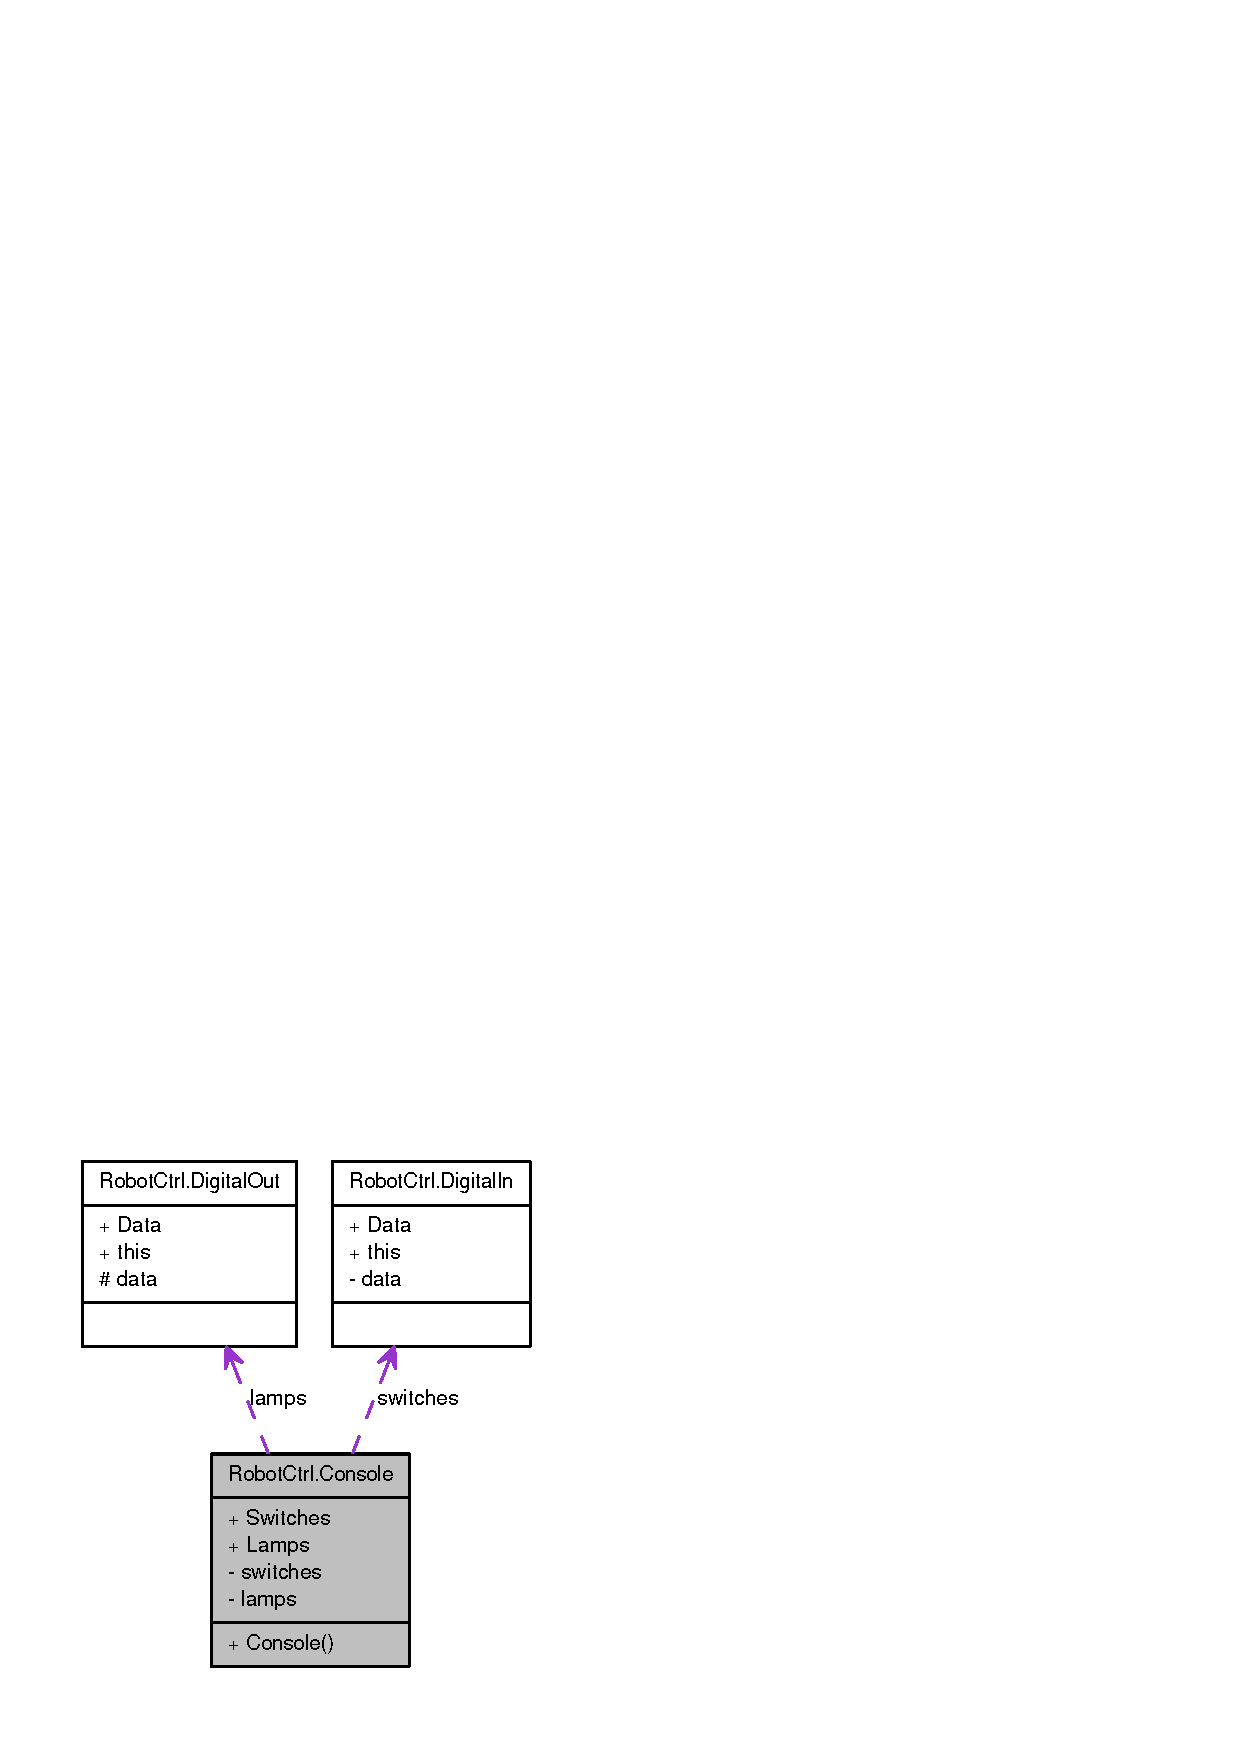
\includegraphics[width=258pt]{class_robot_ctrl_1_1_console__coll__graph}
\end{center}
\end{figure}
\subsection*{Öffentliche Methoden}
\begin{DoxyCompactItemize}
\item 
\hypertarget{class_robot_ctrl_1_1_console_a635815d24705bd6de640c1594554962e}{
{\bfseries Console} (RunMode mode)}
\label{class_robot_ctrl_1_1_console_a635815d24705bd6de640c1594554962e}

\end{DoxyCompactItemize}
\subsection*{Propertys}
\begin{DoxyCompactItemize}
\item 
\hypertarget{class_robot_ctrl_1_1_console_a6bda1a70d35ecd46bdf21be13745932c}{
\hyperlink{class_robot_ctrl_1_1_digital_in}{DigitalIn} {\bfseries Switches}\hspace{0.3cm}{\ttfamily  \mbox{[}get\mbox{]}}}
\label{class_robot_ctrl_1_1_console_a6bda1a70d35ecd46bdf21be13745932c}

\item 
\hypertarget{class_robot_ctrl_1_1_console_a8d77cea764f4a4e2c4692e5776b7ded8}{
\hyperlink{class_robot_ctrl_1_1_digital_out}{DigitalOut} {\bfseries Lamps}\hspace{0.3cm}{\ttfamily  \mbox{[}get\mbox{]}}}
\label{class_robot_ctrl_1_1_console_a8d77cea764f4a4e2c4692e5776b7ded8}

\end{DoxyCompactItemize}


Die Dokumentation für diese Klasse wurde erzeugt aufgrund der Datei:\begin{DoxyCompactItemize}
\item 
Console.cs\end{DoxyCompactItemize}

\hypertarget{class_robot_view_1_1_console_form}{
\section{RobotView.ConsoleForm Klassenreferenz}
\label{class_robot_view_1_1_console_form}\index{RobotView::ConsoleForm@{RobotView::ConsoleForm}}
}


Die Dokumentation für diese Klasse wurde erzeugt aufgrund der Datei:\begin{DoxyCompactItemize}
\item 
ConsoleForm.cs\end{DoxyCompactItemize}

\hypertarget{class_robot_view_1_1_console_view}{
\section{RobotView.ConsoleView Klassenreferenz}
\label{class_robot_view_1_1_console_view}\index{RobotView::ConsoleView@{RobotView::ConsoleView}}
}


Zusammengehörigkeiten von RobotView.ConsoleView:\nopagebreak
\begin{figure}[H]
\begin{center}
\leavevmode
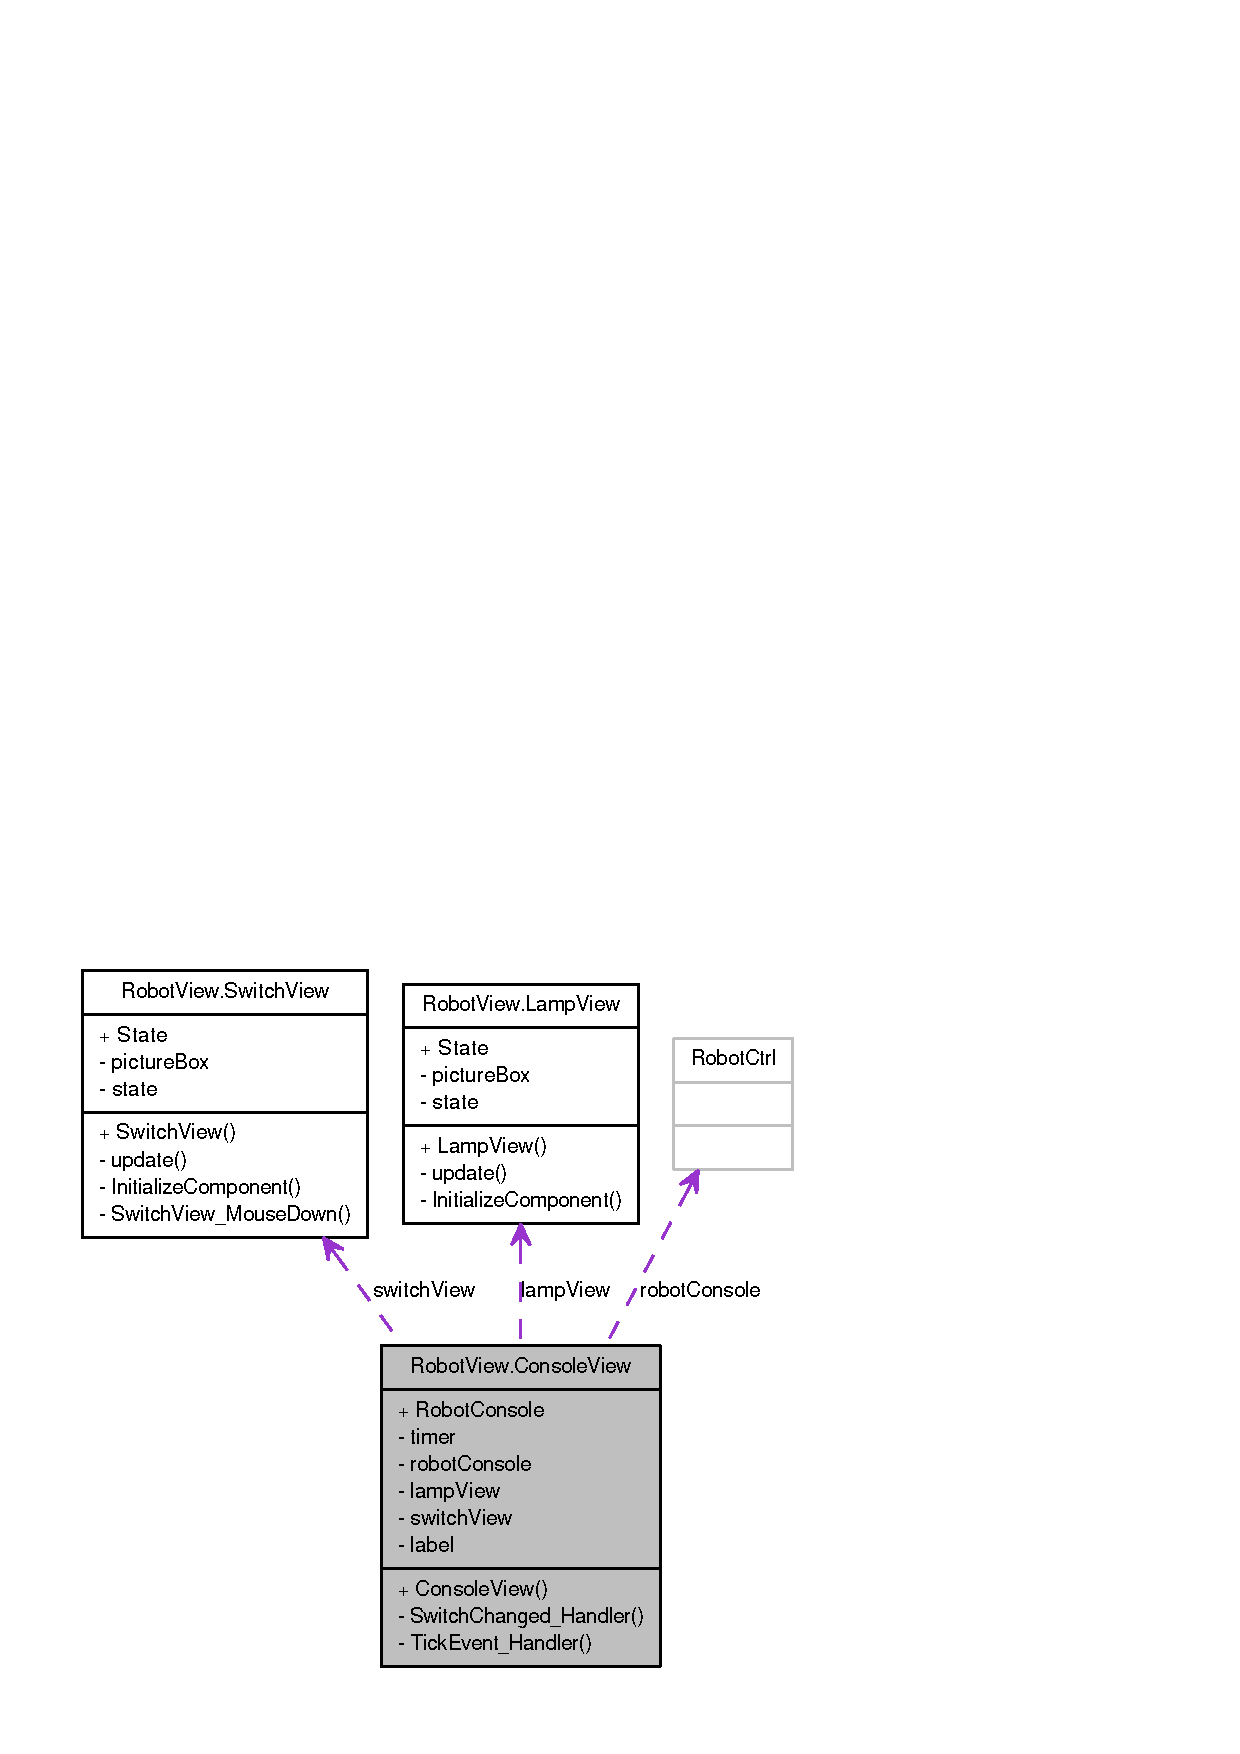
\includegraphics[width=384pt]{class_robot_view_1_1_console_view__coll__graph}
\end{center}
\end{figure}
\subsection*{Propertys}
\begin{DoxyCompactItemize}
\item 
\hypertarget{class_robot_view_1_1_console_view_a699a62faa0e0c66c3fedba5abd70313a}{
\hyperlink{class_robot_ctrl_1_1_console}{RobotCtrl.Console} {\bfseries RobotConsole}\hspace{0.3cm}{\ttfamily  \mbox{[}set\mbox{]}}}
\label{class_robot_view_1_1_console_view_a699a62faa0e0c66c3fedba5abd70313a}

\end{DoxyCompactItemize}


Die Dokumentation für diese Klasse wurde erzeugt aufgrund der Datei:\begin{DoxyCompactItemize}
\item 
ConsoleView.cs\end{DoxyCompactItemize}

\hypertarget{class_robot_ctrl_1_1_digital_in}{
\section{RobotCtrl.DigitalIn Klassenreferenz}
\label{class_robot_ctrl_1_1_digital_in}\index{RobotCtrl::DigitalIn@{RobotCtrl::DigitalIn}}
}


Klassendiagramm für RobotCtrl.DigitalIn:\nopagebreak
\begin{figure}[H]
\begin{center}
\leavevmode
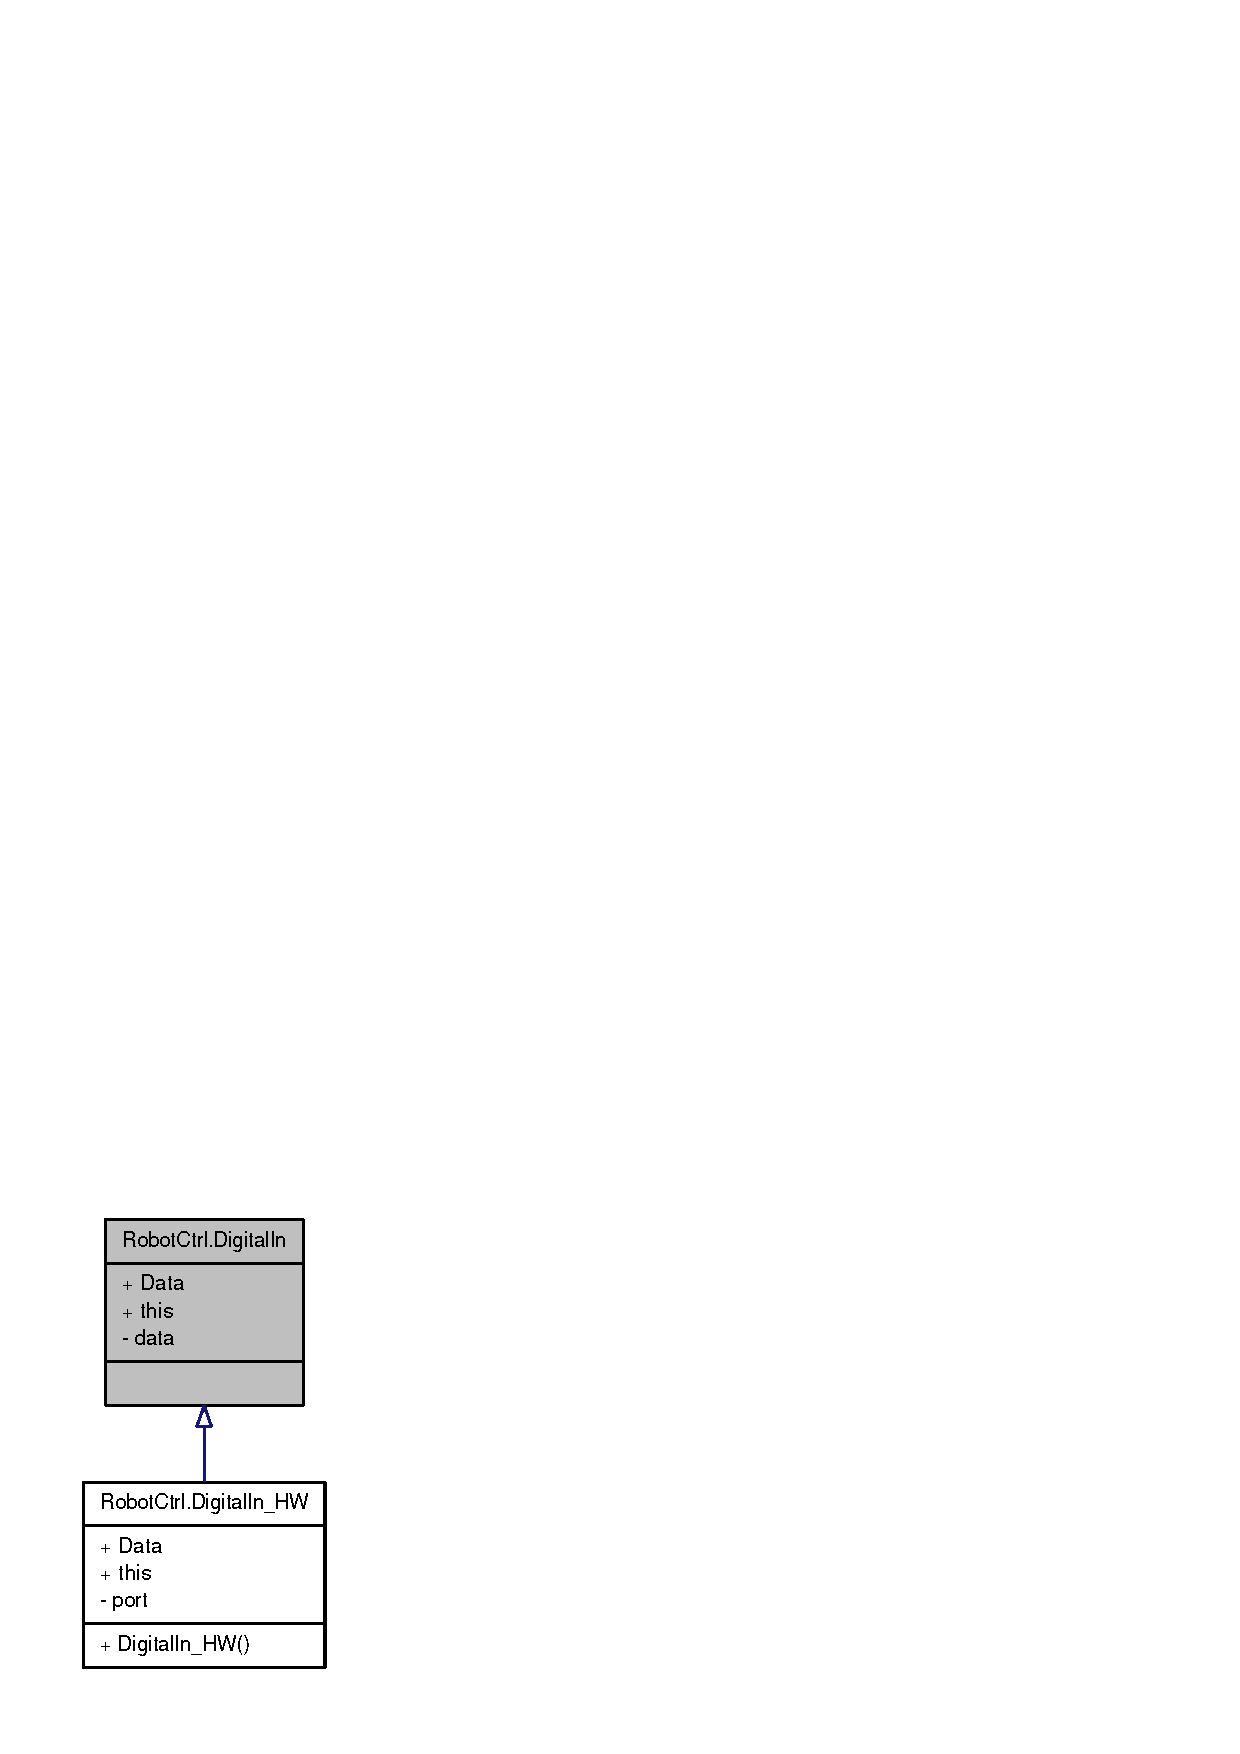
\includegraphics[width=160pt]{class_robot_ctrl_1_1_digital_in__inherit__graph}
\end{center}
\end{figure}
\subsection*{Propertys}
\begin{DoxyCompactItemize}
\item 
\hypertarget{class_robot_ctrl_1_1_digital_in_a9f730b21d4845684a1e085293d2cba50}{
virtual int {\bfseries Data}\hspace{0.3cm}{\ttfamily  \mbox{[}get, set\mbox{]}}}
\label{class_robot_ctrl_1_1_digital_in_a9f730b21d4845684a1e085293d2cba50}

\item 
\hypertarget{class_robot_ctrl_1_1_digital_in_adabed7783bc3ad5603e1adbf2bc37484}{
virtual bool {\bfseries this} \mbox{[}int index\mbox{]}\hspace{0.3cm}{\ttfamily  \mbox{[}get, set\mbox{]}}}
\label{class_robot_ctrl_1_1_digital_in_adabed7783bc3ad5603e1adbf2bc37484}

\end{DoxyCompactItemize}


Die Dokumentation für diese Klasse wurde erzeugt aufgrund der Datei:\begin{DoxyCompactItemize}
\item 
DigitalIn.cs\end{DoxyCompactItemize}

\hypertarget{class_robot_ctrl_1_1_digital_in___h_w}{
\section{RobotCtrl.DigitalIn\_\-HW Klassenreferenz}
\label{class_robot_ctrl_1_1_digital_in___h_w}\index{RobotCtrl::DigitalIn\_\-HW@{RobotCtrl::DigitalIn\_\-HW}}
}


Klassendiagramm für RobotCtrl.DigitalIn\_\-HW:\nopagebreak
\begin{figure}[H]
\begin{center}
\leavevmode
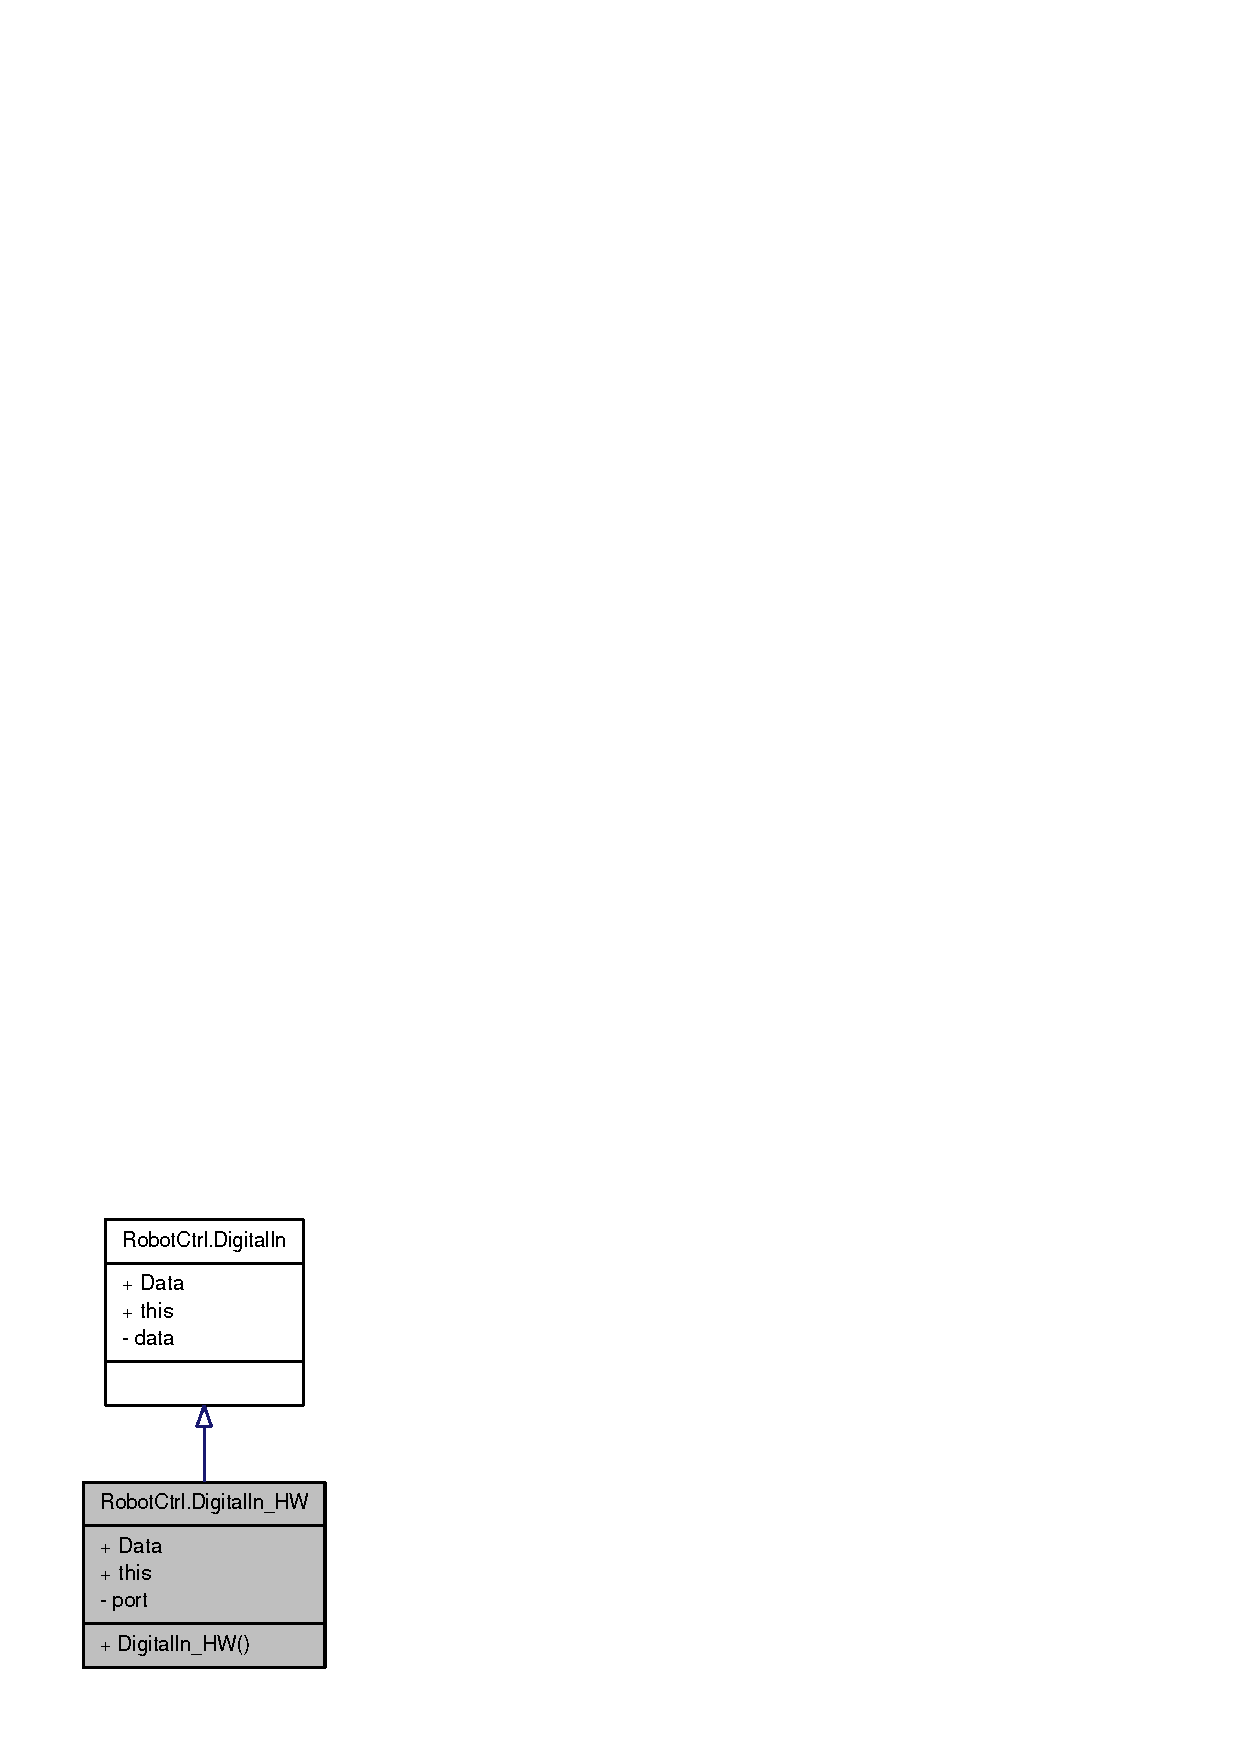
\includegraphics[width=160pt]{class_robot_ctrl_1_1_digital_in___h_w__inherit__graph}
\end{center}
\end{figure}


Zusammengehörigkeiten von RobotCtrl.DigitalIn\_\-HW:\nopagebreak
\begin{figure}[H]
\begin{center}
\leavevmode
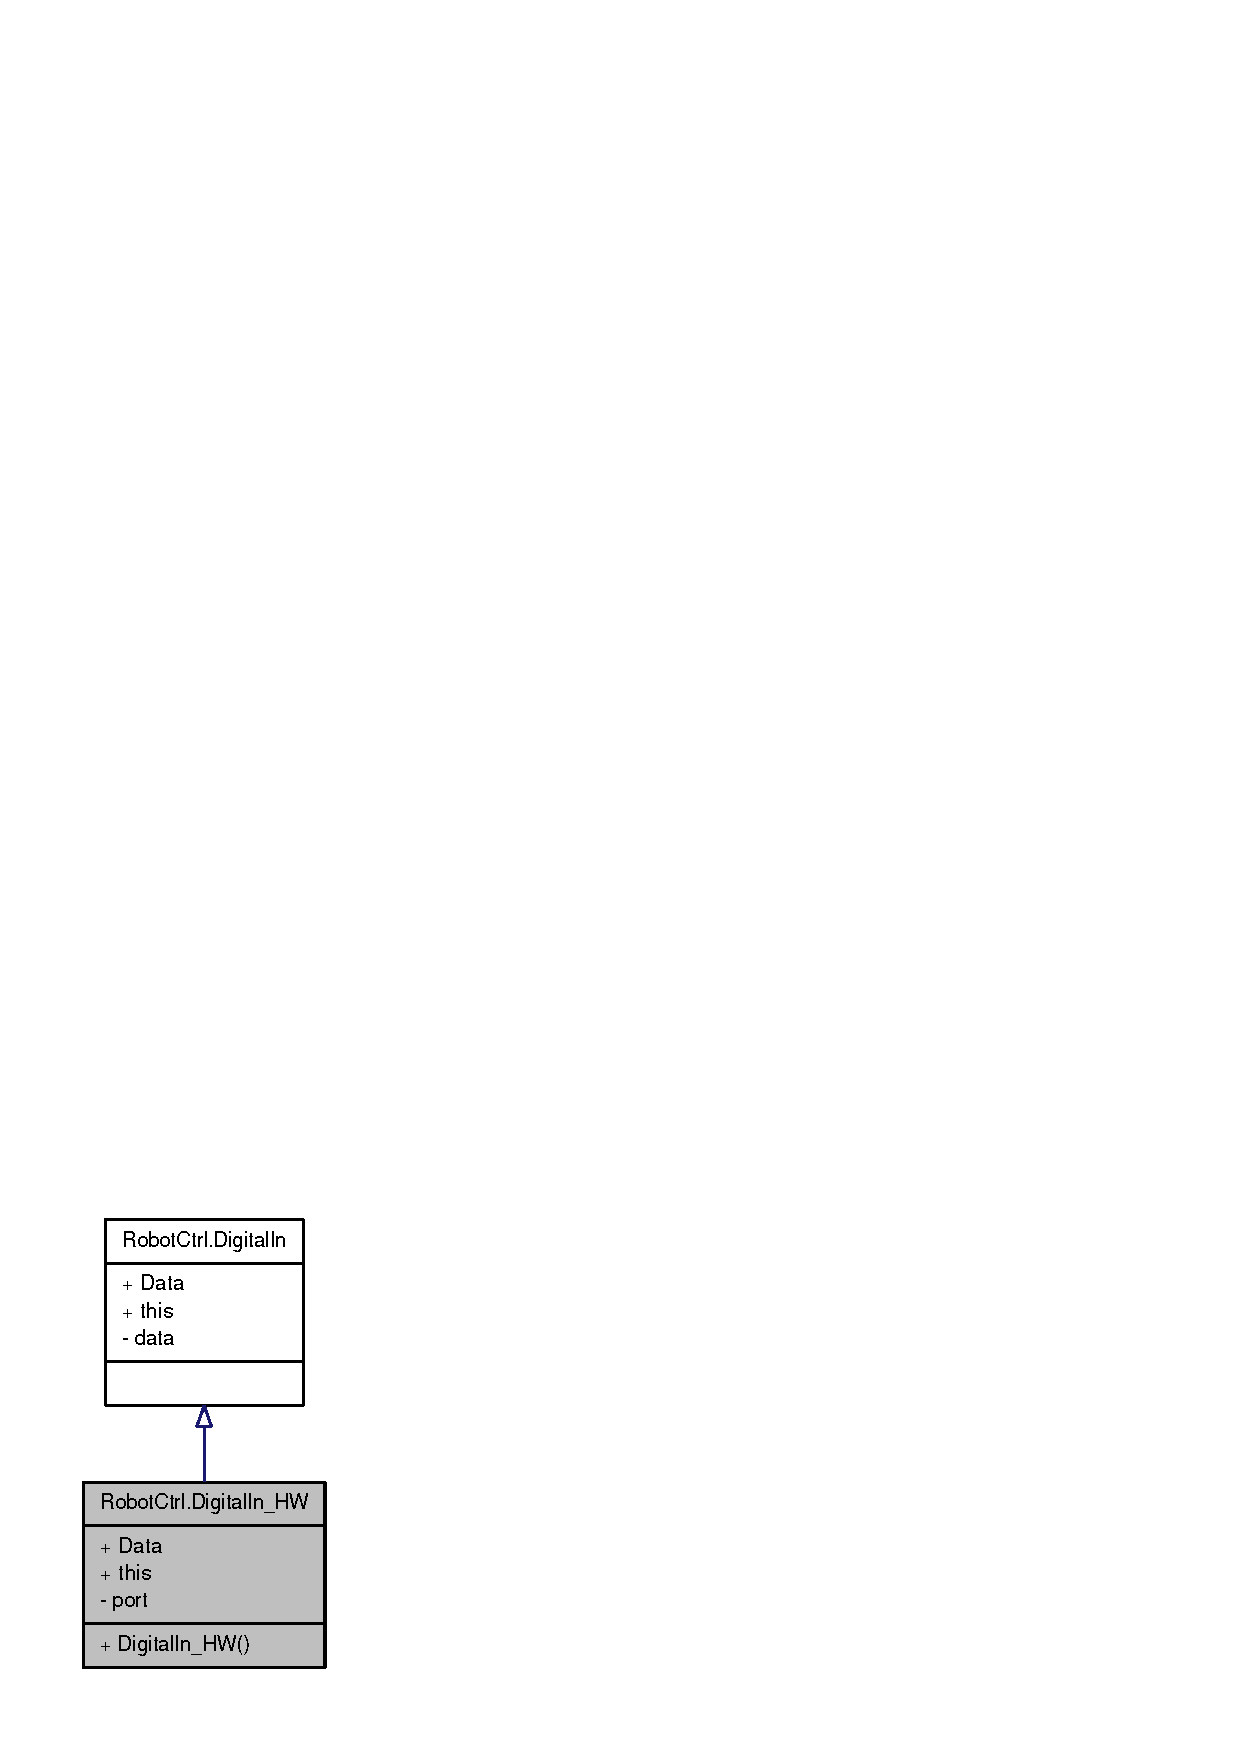
\includegraphics[width=160pt]{class_robot_ctrl_1_1_digital_in___h_w__coll__graph}
\end{center}
\end{figure}
\subsection*{Öffentliche Methoden}
\begin{DoxyCompactItemize}
\item 
\hypertarget{class_robot_ctrl_1_1_digital_in___h_w_a50234a4b44c4c522abe6565a3111309e}{
{\bfseries DigitalIn\_\-HW} (int port)}
\label{class_robot_ctrl_1_1_digital_in___h_w_a50234a4b44c4c522abe6565a3111309e}

\end{DoxyCompactItemize}
\subsection*{Propertys}
\begin{DoxyCompactItemize}
\item 
\hypertarget{class_robot_ctrl_1_1_digital_in___h_w_a22093ed6e3a1b15bbb0406fd56d9b0cc}{
override int {\bfseries Data}\hspace{0.3cm}{\ttfamily  \mbox{[}get\mbox{]}}}
\label{class_robot_ctrl_1_1_digital_in___h_w_a22093ed6e3a1b15bbb0406fd56d9b0cc}

\item 
\hypertarget{class_robot_ctrl_1_1_digital_in___h_w_a1197c7dee03f1a9844a5824e3c6e0941}{
override bool {\bfseries this} \mbox{[}int bit\mbox{]}\hspace{0.3cm}{\ttfamily  \mbox{[}get\mbox{]}}}
\label{class_robot_ctrl_1_1_digital_in___h_w_a1197c7dee03f1a9844a5824e3c6e0941}

\end{DoxyCompactItemize}


Die Dokumentation für diese Klasse wurde erzeugt aufgrund der Datei:\begin{DoxyCompactItemize}
\item 
DigitalIn\_\-HW.cs\end{DoxyCompactItemize}

\hypertarget{class_test___lamp_view_1_1_digital_in_event_arg}{
\section{Test\_\-LampView.DigitalInEventArg Klassenreferenz}
\label{class_test___lamp_view_1_1_digital_in_event_arg}\index{Test\_\-LampView::DigitalInEventArg@{Test\_\-LampView::DigitalInEventArg}}
}
\subsection*{Öffentliche Methoden}
\begin{DoxyCompactItemize}
\item 
\hypertarget{class_test___lamp_view_1_1_digital_in_event_arg_aa6c7168600403e69cb571cc76094ecfe}{
{\bfseries DigitalInEventArg} (int bitNumber)}
\label{class_test___lamp_view_1_1_digital_in_event_arg_aa6c7168600403e69cb571cc76094ecfe}

\end{DoxyCompactItemize}
\subsection*{Propertys}
\begin{DoxyCompactItemize}
\item 
\hypertarget{class_test___lamp_view_1_1_digital_in_event_arg_afc917ab4e6171a391729b90baec28168}{
int {\bfseries BitNumber}\hspace{0.3cm}{\ttfamily  \mbox{[}get\mbox{]}}}
\label{class_test___lamp_view_1_1_digital_in_event_arg_afc917ab4e6171a391729b90baec28168}

\end{DoxyCompactItemize}


Die Dokumentation für diese Klasse wurde erzeugt aufgrund der Datei:\begin{DoxyCompactItemize}
\item 
Test\_\-LampView\_\-Form.cs\end{DoxyCompactItemize}

\hypertarget{class_robot_ctrl_1_1_digital_out}{
\section{RobotCtrl.DigitalOut Klassenreferenz}
\label{class_robot_ctrl_1_1_digital_out}\index{RobotCtrl::DigitalOut@{RobotCtrl::DigitalOut}}
}


Klassendiagramm für RobotCtrl.DigitalOut:\nopagebreak
\begin{figure}[H]
\begin{center}
\leavevmode
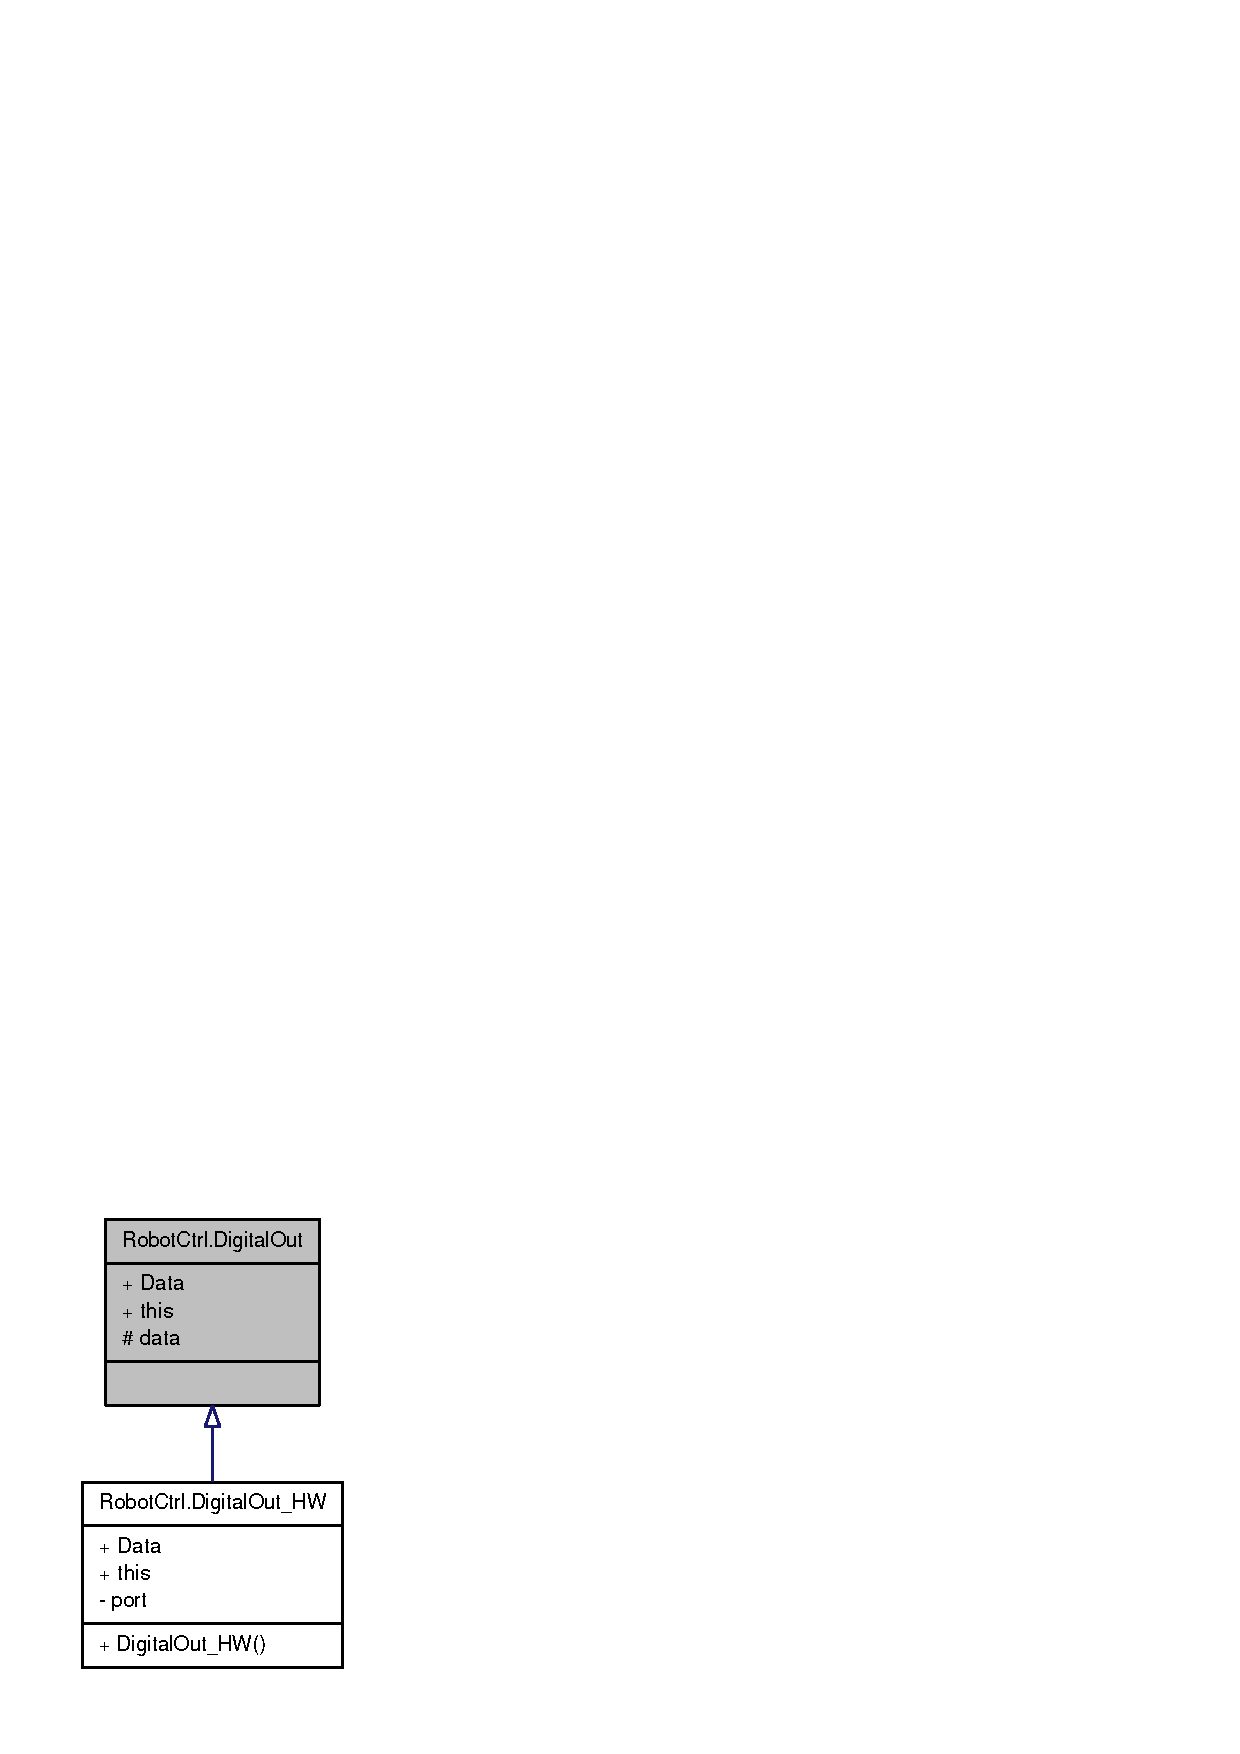
\includegraphics[width=168pt]{class_robot_ctrl_1_1_digital_out__inherit__graph}
\end{center}
\end{figure}
\subsection*{Geschützte Attribute}
\begin{DoxyCompactItemize}
\item 
\hypertarget{class_robot_ctrl_1_1_digital_out_aefd56fa4fcdd5ba7eb3f34545cc090a6}{
int {\bfseries data}}
\label{class_robot_ctrl_1_1_digital_out_aefd56fa4fcdd5ba7eb3f34545cc090a6}

\end{DoxyCompactItemize}
\subsection*{Propertys}
\begin{DoxyCompactItemize}
\item 
\hypertarget{class_robot_ctrl_1_1_digital_out_a4c85a4bab149666840e9a551f62b6305}{
virtual int {\bfseries Data}\hspace{0.3cm}{\ttfamily  \mbox{[}get, set\mbox{]}}}
\label{class_robot_ctrl_1_1_digital_out_a4c85a4bab149666840e9a551f62b6305}

\item 
\hypertarget{class_robot_ctrl_1_1_digital_out_a4f57b73a7591bb053e7025eebb26d577}{
virtual bool {\bfseries this} \mbox{[}int index\mbox{]}\hspace{0.3cm}{\ttfamily  \mbox{[}get, set\mbox{]}}}
\label{class_robot_ctrl_1_1_digital_out_a4f57b73a7591bb053e7025eebb26d577}

\end{DoxyCompactItemize}


Die Dokumentation für diese Klasse wurde erzeugt aufgrund der Datei:\begin{DoxyCompactItemize}
\item 
DigitalOut.cs\end{DoxyCompactItemize}

\hypertarget{class_robot_ctrl_1_1_digital_out___h_w}{
\section{RobotCtrl.DigitalOut\_\-HW Klassenreferenz}
\label{class_robot_ctrl_1_1_digital_out___h_w}\index{RobotCtrl::DigitalOut\_\-HW@{RobotCtrl::DigitalOut\_\-HW}}
}


Klassendiagramm für RobotCtrl.DigitalOut\_\-HW:\nopagebreak
\begin{figure}[H]
\begin{center}
\leavevmode
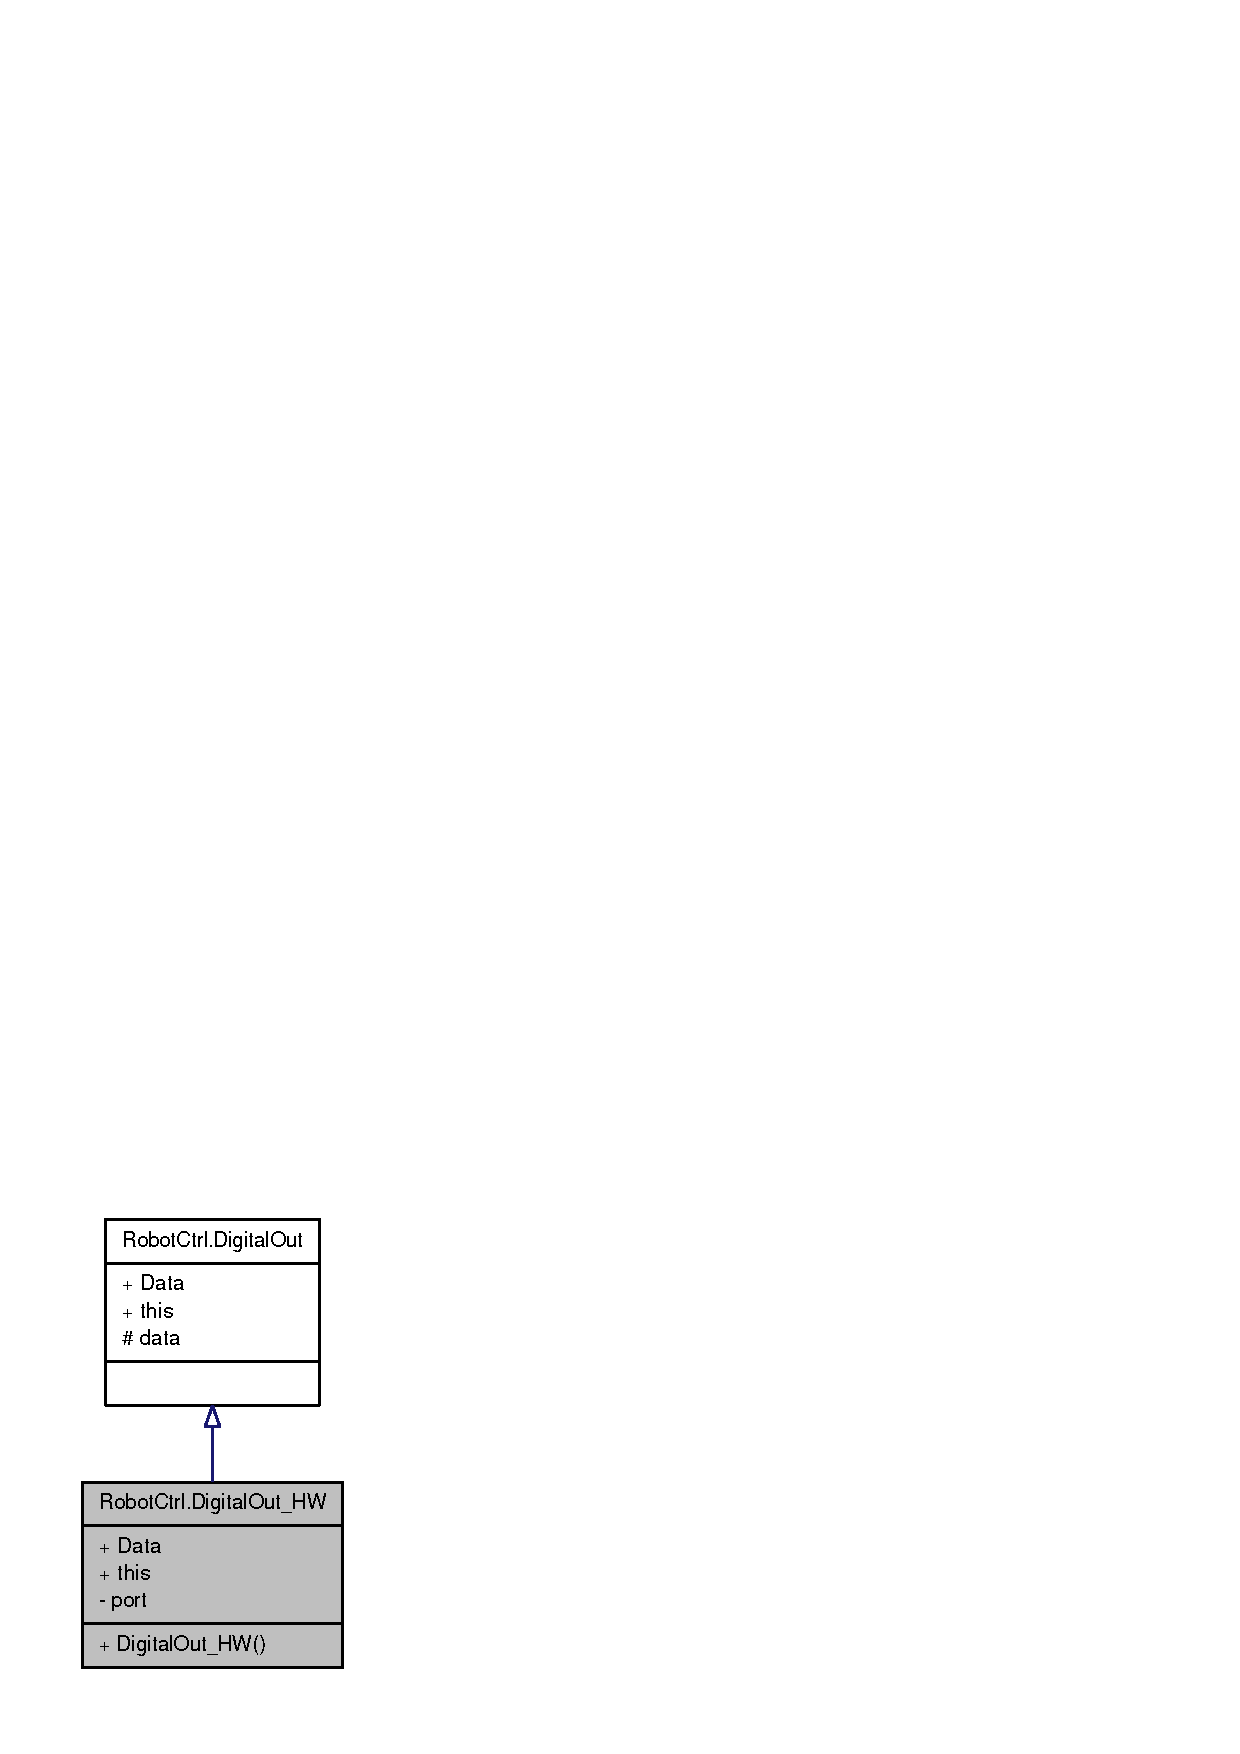
\includegraphics[width=168pt]{class_robot_ctrl_1_1_digital_out___h_w__inherit__graph}
\end{center}
\end{figure}


Zusammengehörigkeiten von RobotCtrl.DigitalOut\_\-HW:\nopagebreak
\begin{figure}[H]
\begin{center}
\leavevmode
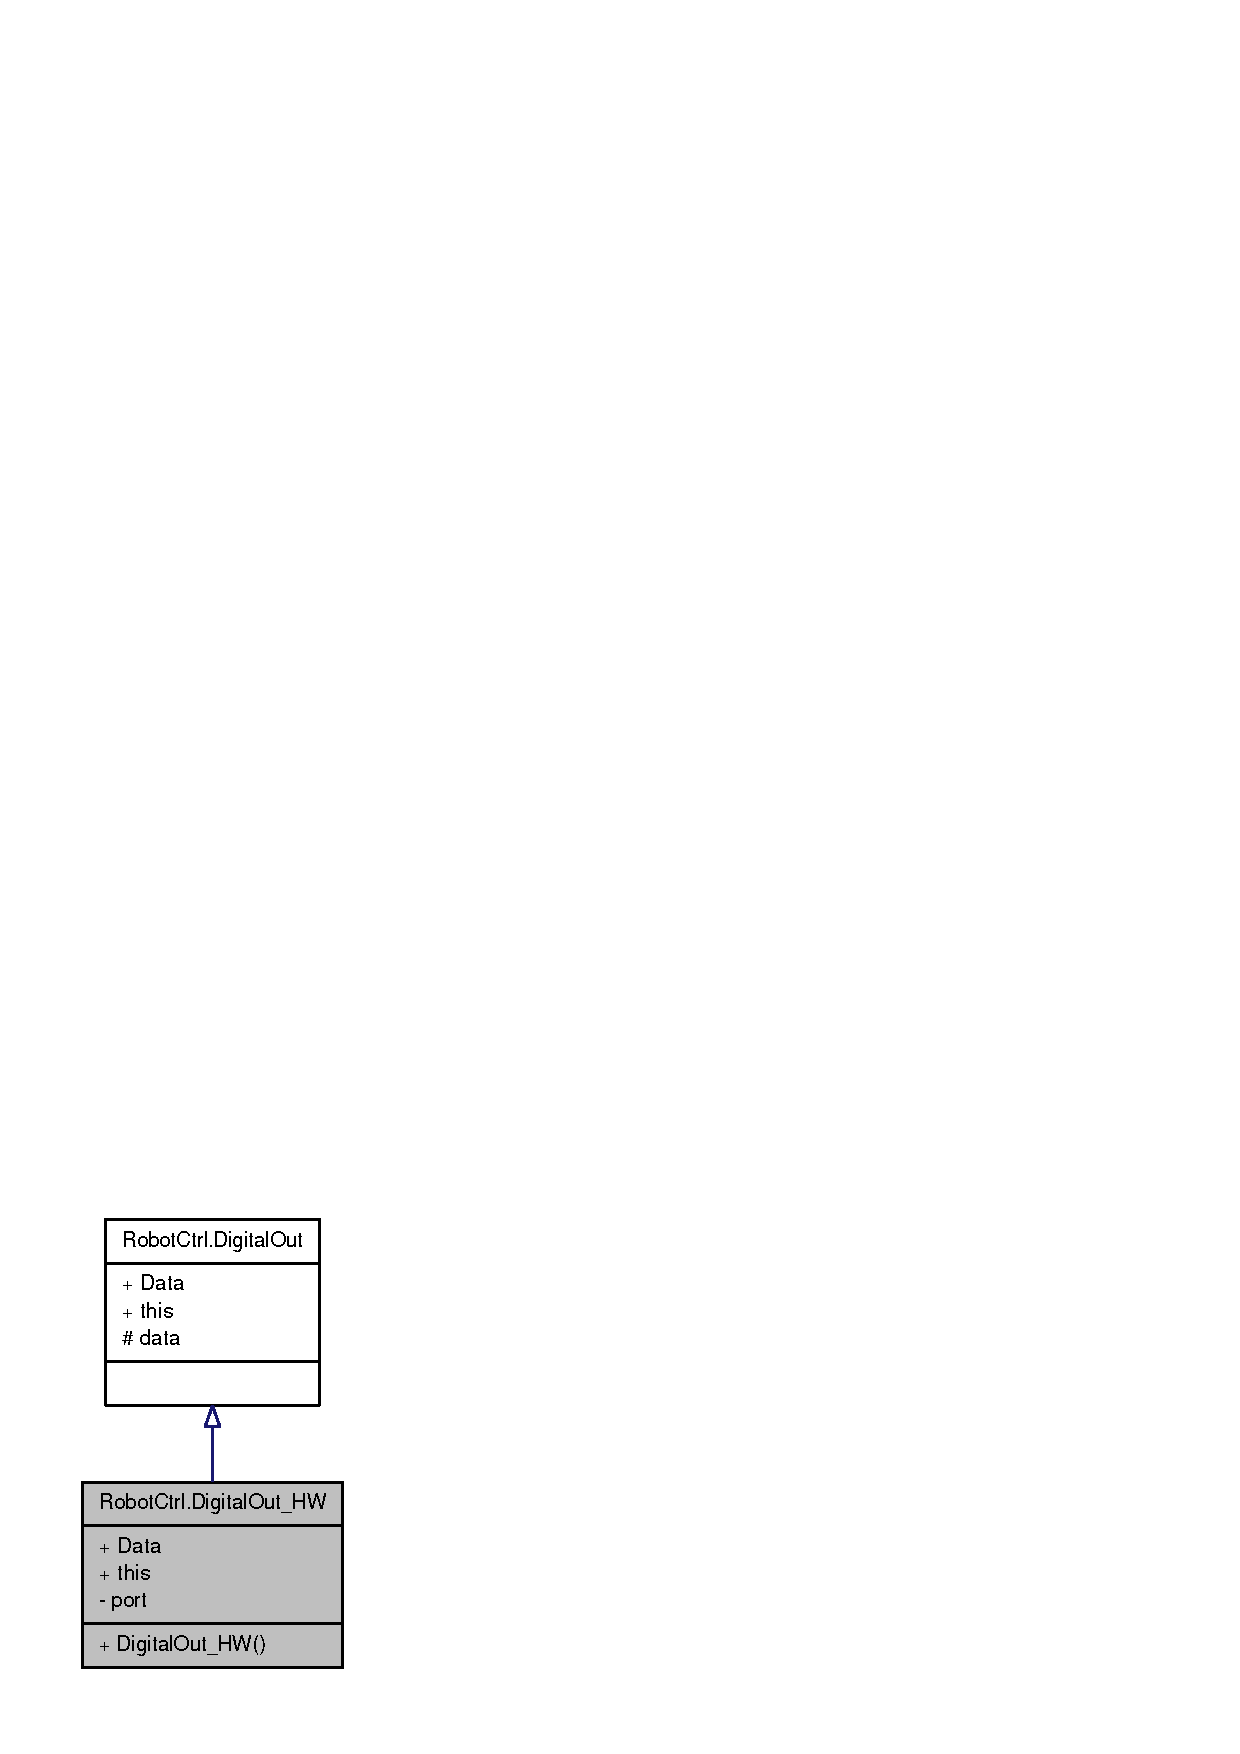
\includegraphics[width=168pt]{class_robot_ctrl_1_1_digital_out___h_w__coll__graph}
\end{center}
\end{figure}
\subsection*{Öffentliche Methoden}
\begin{DoxyCompactItemize}
\item 
\hypertarget{class_robot_ctrl_1_1_digital_out___h_w_ae26dd8f2e439fa83f3afb1c8fad3e266}{
{\bfseries DigitalOut\_\-HW} (int port)}
\label{class_robot_ctrl_1_1_digital_out___h_w_ae26dd8f2e439fa83f3afb1c8fad3e266}

\end{DoxyCompactItemize}
\subsection*{Propertys}
\begin{DoxyCompactItemize}
\item 
\hypertarget{class_robot_ctrl_1_1_digital_out___h_w_ae374c259f09079b63f2bb6533e6ce5de}{
override int {\bfseries Data}\hspace{0.3cm}{\ttfamily  \mbox{[}get\mbox{]}}}
\label{class_robot_ctrl_1_1_digital_out___h_w_ae374c259f09079b63f2bb6533e6ce5de}

\item 
\hypertarget{class_robot_ctrl_1_1_digital_out___h_w_a76f77544e88287efb3b2f273429b2ff0}{
override bool {\bfseries this} \mbox{[}int bit\mbox{]}\hspace{0.3cm}{\ttfamily  \mbox{[}get\mbox{]}}}
\label{class_robot_ctrl_1_1_digital_out___h_w_a76f77544e88287efb3b2f273429b2ff0}

\end{DoxyCompactItemize}


Die Dokumentation für diese Klasse wurde erzeugt aufgrund der Datei:\begin{DoxyCompactItemize}
\item 
DigitalOut\_\-HW.cs\end{DoxyCompactItemize}

\hypertarget{class_test___lamp_view_1_1_digital_out_event_arg}{
\section{Test\_\-LampView.DigitalOutEventArg Klassenreferenz}
\label{class_test___lamp_view_1_1_digital_out_event_arg}\index{Test\_\-LampView::DigitalOutEventArg@{Test\_\-LampView::DigitalOutEventArg}}
}
\subsection*{Öffentliche Methoden}
\begin{DoxyCompactItemize}
\item 
\hypertarget{class_test___lamp_view_1_1_digital_out_event_arg_a1f74109a1a14c365be62d74fb441be4c}{
{\bfseries DigitalOutEventArg} (int bitNumber)}
\label{class_test___lamp_view_1_1_digital_out_event_arg_a1f74109a1a14c365be62d74fb441be4c}

\end{DoxyCompactItemize}
\subsection*{Propertys}
\begin{DoxyCompactItemize}
\item 
\hypertarget{class_test___lamp_view_1_1_digital_out_event_arg_a2e91db32b8a2b3506e6ee4643d5a5a09}{
int {\bfseries BitNumber}\hspace{0.3cm}{\ttfamily  \mbox{[}get\mbox{]}}}
\label{class_test___lamp_view_1_1_digital_out_event_arg_a2e91db32b8a2b3506e6ee4643d5a5a09}

\end{DoxyCompactItemize}


Die Dokumentation für diese Klasse wurde erzeugt aufgrund der Datei:\begin{DoxyCompactItemize}
\item 
Test-\/LampView/Form1.cs\end{DoxyCompactItemize}

\hypertarget{class_robot_ctrl_1_1_drive}{
\section{RobotCtrl.Drive Klassenreferenz}
\label{class_robot_ctrl_1_1_drive}\index{RobotCtrl::Drive@{RobotCtrl::Drive}}
}


\hyperlink{class_robot_ctrl_1_1_drive}{Drive}, damit der Roboter herumfahren kann.  




Zusammengehörigkeiten von RobotCtrl.Drive:\subsection*{Öffentliche Methoden}
\begin{DoxyCompactItemize}
\item 
\hyperlink{class_robot_ctrl_1_1_drive_a76fb877ffa6c136983d59ab7e8f2995b}{Drive} (\hyperlink{class_robot_ctrl_1_1_robot}{Robot} robot, RunMode runMode)
\item 
void \hyperlink{class_robot_ctrl_1_1_drive_ad79a30093b989b2b701e07d1caf7fecc}{Reset} ()
\item 
void \hyperlink{class_robot_ctrl_1_1_drive_af902934c2a3f12ef34bc55bb1827cc13}{Close} ()
\item 
void \hyperlink{class_robot_ctrl_1_1_drive_a39fa32f34e3cd62b99b502948c416897}{Stop} ()
\item 
void \hyperlink{class_robot_ctrl_1_1_drive_aaa24d6438ff31a1dea837423c4047096}{Halt} ()
\item 
void \hyperlink{class_robot_ctrl_1_1_drive_a16bd2f585366688a74f4ad550ffc2ec6}{WaitDone} ()
\item 
void \hyperlink{class_robot_ctrl_1_1_drive_aecd1cd44e2e89488866b58c7753bb4d5}{RunPause} (double pauseTimeSeconds)
\item 
void \hyperlink{class_robot_ctrl_1_1_drive_a62eb0b9939a24046a6dd0372cae3758b}{RunLine} (double length, double speed, double runAcceleration)
\item 
void \hyperlink{class_robot_ctrl_1_1_drive_a5b1a280fceb771ccad2e19d96e5c4ef3}{RunArcLeft} (double radius, double angle, double speed, double runAcceleration)
\item 
void \hyperlink{class_robot_ctrl_1_1_drive_a6ef57fad047014b11a60f76c74a4b74c}{RunArcRight} (double runRadius, double runAngle, double runSpeed, double runAcceleration)
\item 
void \hyperlink{class_robot_ctrl_1_1_drive_a2c49e16e45f1db8c54160cd978d501ea}{RunTurn} (double runAngle, double runSpeed, double runAcceleration)
\item 
void \hyperlink{class_robot_ctrl_1_1_drive_ab83216b1690ed4b93b412984318ad345}{RunContourLeft} (double distance, double runSpeed, double runAcceleration)
\end{DoxyCompactItemize}
\subsection*{Propertys}
\begin{DoxyCompactItemize}
\item 
\hyperlink{struct_robot_ctrl_1_1_position_info}{PositionInfo} \hyperlink{class_robot_ctrl_1_1_drive_a422e46eec9edf940ccd3afc5f4fde11e}{Position}\hspace{0.3cm}{\ttfamily  \mbox{[}get, set\mbox{]}}
\item 
bool \hyperlink{class_robot_ctrl_1_1_drive_a208251b538e017abf712b1881a32239a}{Power}\hspace{0.3cm}{\ttfamily  \mbox{[}set\mbox{]}}
\item 
\hyperlink{struct_robot_ctrl_1_1_drive_info}{DriveInfo} \hyperlink{class_robot_ctrl_1_1_drive_a0e6f8392e835c0789ce8cc9ce1a91ed2}{Info}\hspace{0.3cm}{\ttfamily  \mbox{[}get\mbox{]}}
\item 
bool \hyperlink{class_robot_ctrl_1_1_drive_a5c86389ee2d397c20edf926a21326399}{Done}\hspace{0.3cm}{\ttfamily  \mbox{[}get\mbox{]}}
\end{DoxyCompactItemize}


\subsection{Ausführliche Beschreibung}
\hyperlink{class_robot_ctrl_1_1_drive}{Drive}, damit der Roboter herumfahren kann. 

\subsection{Beschreibung der Konstruktoren und Destruktoren}
\hypertarget{class_robot_ctrl_1_1_drive_a76fb877ffa6c136983d59ab7e8f2995b}{
\index{RobotCtrl::Drive@{RobotCtrl::Drive}!Drive@{Drive}}
\index{Drive@{Drive}!RobotCtrl::Drive@{RobotCtrl::Drive}}
\subsubsection[{Drive}]{\setlength{\rightskip}{0pt plus 5cm}RobotCtrl.Drive.Drive ({\bf Robot} {\em robot}, \/  RunMode {\em runMode})}}
\label{class_robot_ctrl_1_1_drive_a76fb877ffa6c136983d59ab7e8f2995b}
Konstruktor f\"{u}r ein \hyperlink{class_robot_ctrl_1_1_drive}{Drive} Objekt.


\begin{DoxyParams}{Parameter}
\item[{\em robot}]Referenz auf einen \hyperlink{class_robot_ctrl_1_1_robot}{Robot} \item[{\em runMode}]enum RunMode \end{DoxyParams}


\subsection{Dokumentation der Elementfunktionen}
\hypertarget{class_robot_ctrl_1_1_drive_af902934c2a3f12ef34bc55bb1827cc13}{
\index{RobotCtrl::Drive@{RobotCtrl::Drive}!Close@{Close}}
\index{Close@{Close}!RobotCtrl::Drive@{RobotCtrl::Drive}}
\subsubsection[{Close}]{\setlength{\rightskip}{0pt plus 5cm}void RobotCtrl.Drive.Close ()}}
\label{class_robot_ctrl_1_1_drive_af902934c2a3f12ef34bc55bb1827cc13}
Methode resetiert das referenzierte \hyperlink{class_robot_ctrl_1_1_drive_ctrl}{DriveCtrl} und beendet die aktuelle Fahrt des \hyperlink{class_robot_ctrl_1_1_robot}{Robot}. 

Hier ist ein Graph der zeigt, was diese Funktion aufruft:\nopagebreak
\begin{figure}[H]
\begin{center}
\leavevmode
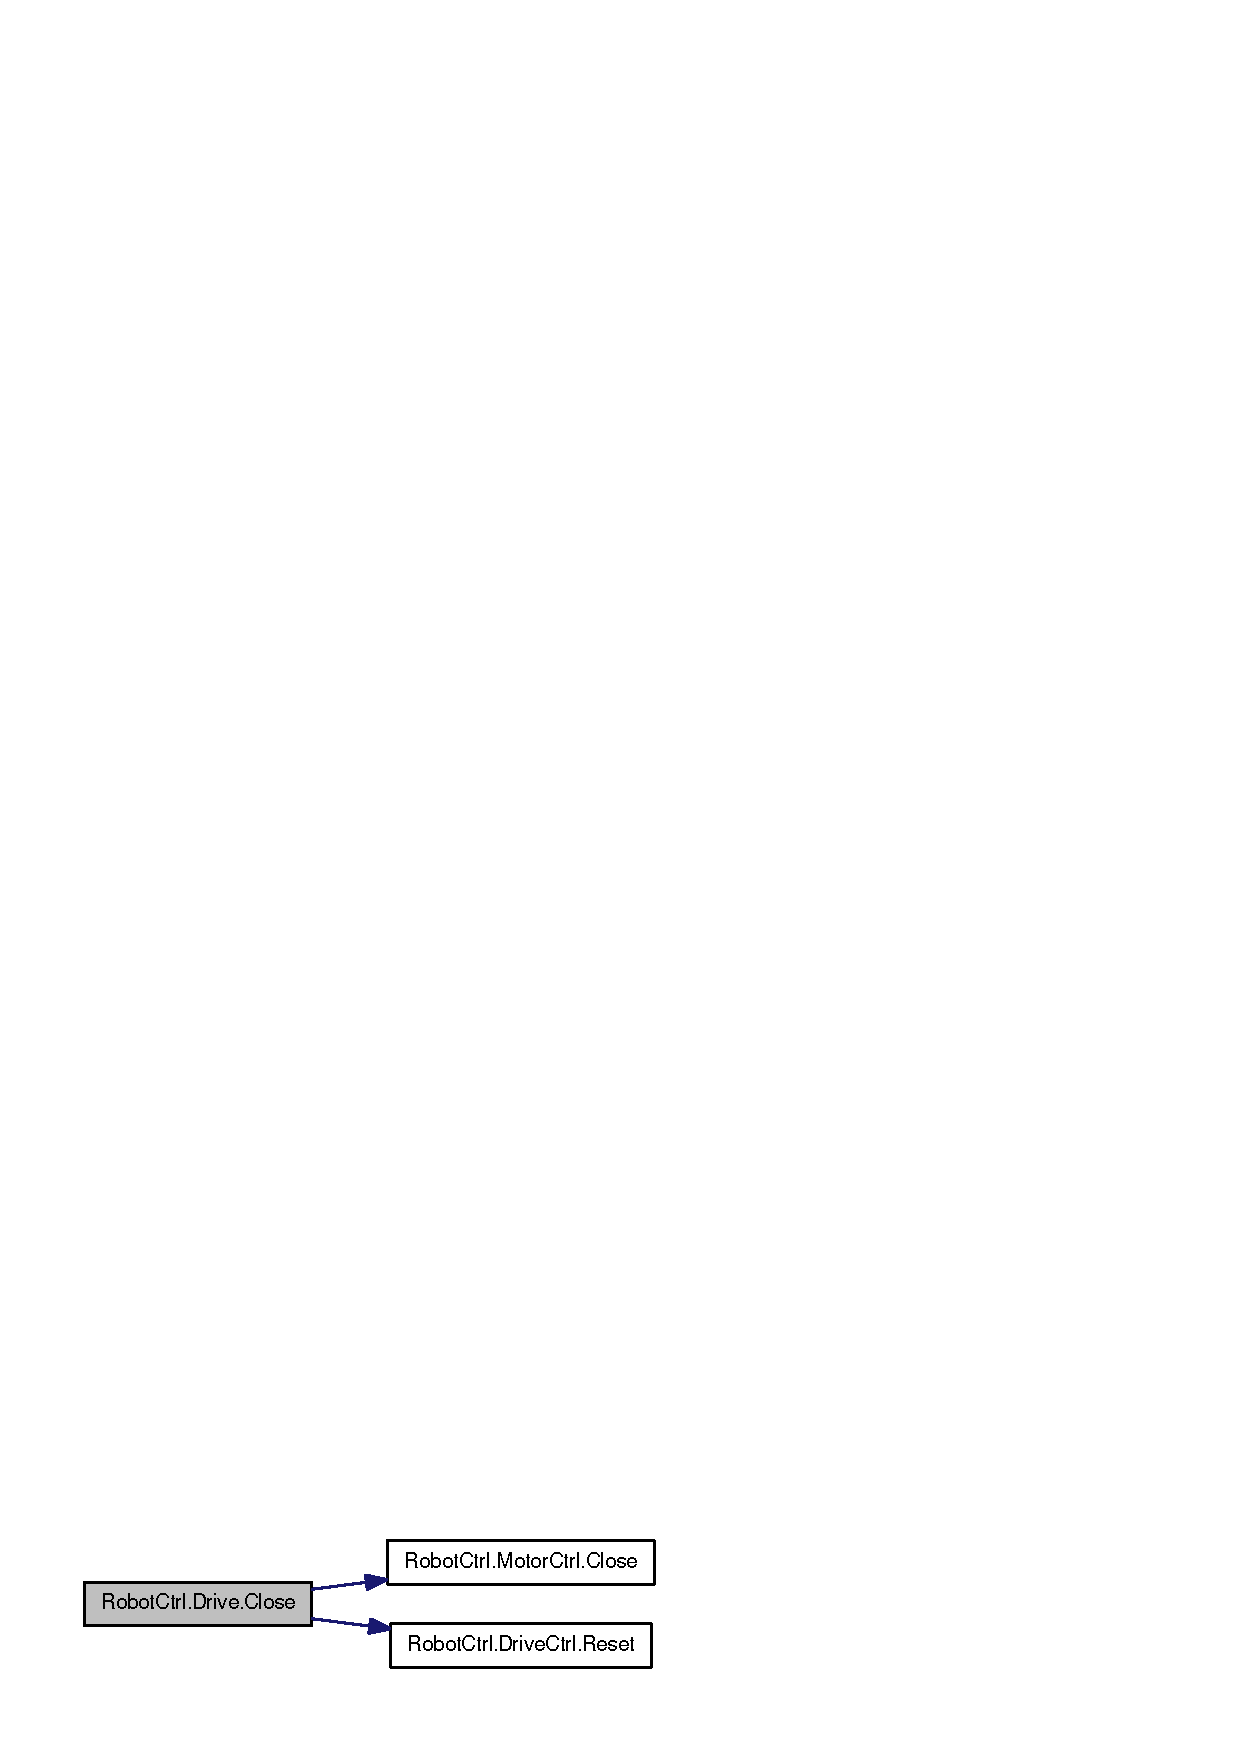
\includegraphics[width=159pt]{class_robot_ctrl_1_1_drive_af902934c2a3f12ef34bc55bb1827cc13_cgraph}
\end{center}
\end{figure}


\hypertarget{class_robot_ctrl_1_1_drive_aaa24d6438ff31a1dea837423c4047096}{
\index{RobotCtrl::Drive@{RobotCtrl::Drive}!Halt@{Halt}}
\index{Halt@{Halt}!RobotCtrl::Drive@{RobotCtrl::Drive}}
\subsubsection[{Halt}]{\setlength{\rightskip}{0pt plus 5cm}void RobotCtrl.Drive.Halt ()}}
\label{class_robot_ctrl_1_1_drive_aaa24d6438ff31a1dea837423c4047096}
Befehl zum Halten des \hyperlink{class_robot_ctrl_1_1_robot}{Robot}. \hypertarget{class_robot_ctrl_1_1_drive_ad79a30093b989b2b701e07d1caf7fecc}{
\index{RobotCtrl::Drive@{RobotCtrl::Drive}!Reset@{Reset}}
\index{Reset@{Reset}!RobotCtrl::Drive@{RobotCtrl::Drive}}
\subsubsection[{Reset}]{\setlength{\rightskip}{0pt plus 5cm}void RobotCtrl.Drive.Reset ()}}
\label{class_robot_ctrl_1_1_drive_ad79a30093b989b2b701e07d1caf7fecc}
Methode resetiert das referenzierte \hyperlink{class_robot_ctrl_1_1_drive_ctrl}{DriveCtrl} 

Hier ist ein Graph der zeigt, was diese Funktion aufruft:\nopagebreak
\begin{figure}[H]
\begin{center}
\leavevmode
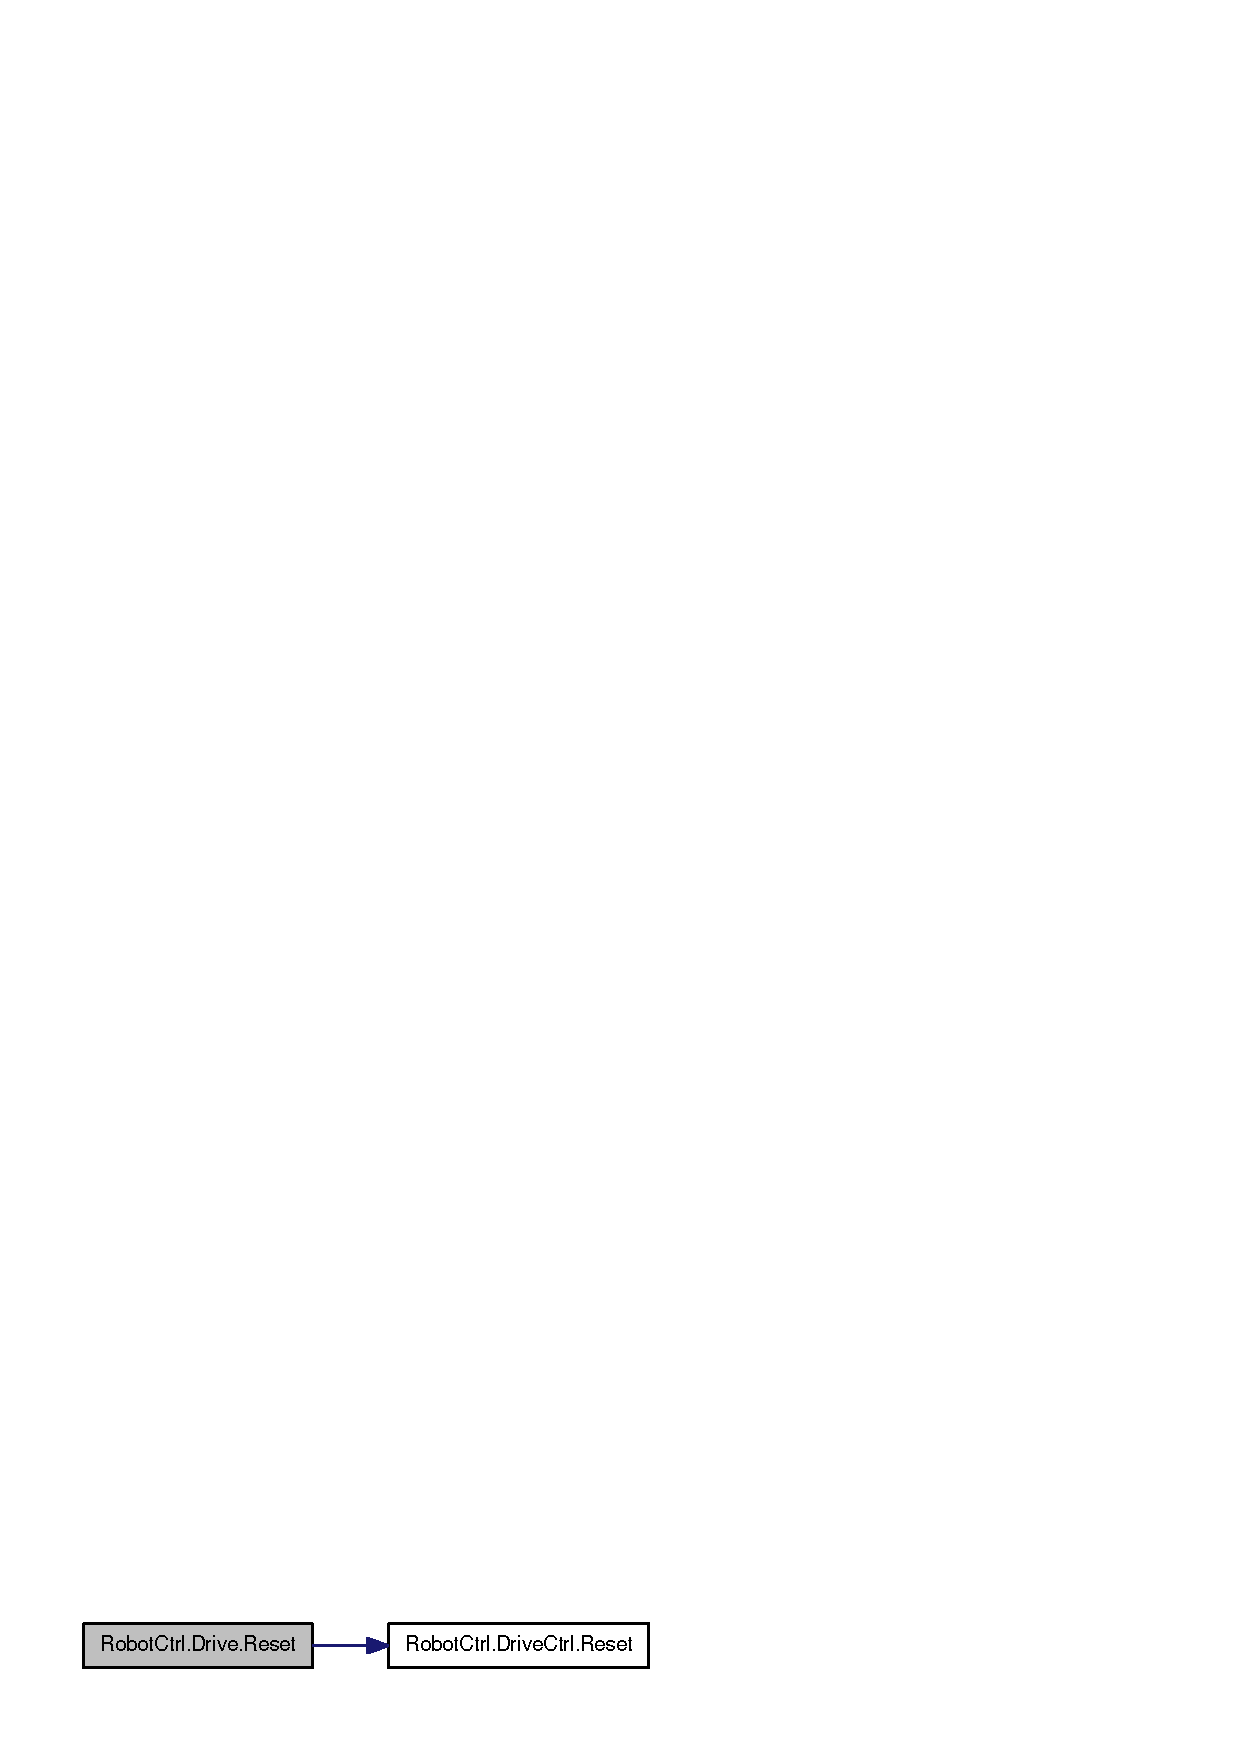
\includegraphics[width=158pt]{class_robot_ctrl_1_1_drive_ad79a30093b989b2b701e07d1caf7fecc_cgraph}
\end{center}
\end{figure}


\hypertarget{class_robot_ctrl_1_1_drive_a5b1a280fceb771ccad2e19d96e5c4ef3}{
\index{RobotCtrl::Drive@{RobotCtrl::Drive}!RunArcLeft@{RunArcLeft}}
\index{RunArcLeft@{RunArcLeft}!RobotCtrl::Drive@{RobotCtrl::Drive}}
\subsubsection[{RunArcLeft}]{\setlength{\rightskip}{0pt plus 5cm}void RobotCtrl.Drive.RunArcLeft (double {\em radius}, \/  double {\em angle}, \/  double {\em speed}, \/  double {\em runAcceleration})}}
\label{class_robot_ctrl_1_1_drive_a5b1a280fceb771ccad2e19d96e5c4ef3}
Methode setzt die zu fahrende \hyperlink{class_robot_ctrl_1_1_track}{Track}. In diesem Fall ist es einen Bogen nach links.


\begin{DoxyParams}{Parameter}
\item[{\em radius}]der Radius des zu fahrenden Bogens \item[{\em angle}]der Winkel des zu fahrenden Bogens \item[{\em speed}]die Geschwindigkeit f\"{u}r die zu fahrende Strecke \item[{\em runAcceleration}]die Beschleunigung auf der Strecke \end{DoxyParams}
\hypertarget{class_robot_ctrl_1_1_drive_a6ef57fad047014b11a60f76c74a4b74c}{
\index{RobotCtrl::Drive@{RobotCtrl::Drive}!RunArcRight@{RunArcRight}}
\index{RunArcRight@{RunArcRight}!RobotCtrl::Drive@{RobotCtrl::Drive}}
\subsubsection[{RunArcRight}]{\setlength{\rightskip}{0pt plus 5cm}void RobotCtrl.Drive.RunArcRight (double {\em runRadius}, \/  double {\em runAngle}, \/  double {\em runSpeed}, \/  double {\em runAcceleration})}}
\label{class_robot_ctrl_1_1_drive_a6ef57fad047014b11a60f76c74a4b74c}
Methode setzt die zu fahrende \hyperlink{class_robot_ctrl_1_1_track}{Track}. In diesem Fall ist es einen Bogen nach rechts.


\begin{DoxyParams}{Parameter}
\item[{\em radius}]der Radius des zu fahrenden Bogens \item[{\em angle}]der Winkel des zu fahrenden Bogens \item[{\em speed}]die Geschwindigkeit f\"{u}r die zu fahrende Strecke \item[{\em runAcceleration}]die Beschleunigung auf der Strecke \end{DoxyParams}
\hypertarget{class_robot_ctrl_1_1_drive_ab83216b1690ed4b93b412984318ad345}{
\index{RobotCtrl::Drive@{RobotCtrl::Drive}!RunContourLeft@{RunContourLeft}}
\index{RunContourLeft@{RunContourLeft}!RobotCtrl::Drive@{RobotCtrl::Drive}}
\subsubsection[{RunContourLeft}]{\setlength{\rightskip}{0pt plus 5cm}void RobotCtrl.Drive.RunContourLeft (double {\em distance}, \/  double {\em runSpeed}, \/  double {\em runAcceleration})}}
\label{class_robot_ctrl_1_1_drive_ab83216b1690ed4b93b412984318ad345}
Methode setzt die zu fahrende \hyperlink{class_robot_ctrl_1_1_track}{Track}. In diesem Fall ist es eine Fahrt um eine Kontur.


\begin{DoxyParams}{Parameter}
\item[{\em distance}]der Abstand zur Kontur \item[{\em runSpeed}]die Geschwindigkeit f\"{u}r die zu fahrende Strecke \item[{\em runAcceleration}]die Beschleunigung auf der Strecke \end{DoxyParams}
\hypertarget{class_robot_ctrl_1_1_drive_a62eb0b9939a24046a6dd0372cae3758b}{
\index{RobotCtrl::Drive@{RobotCtrl::Drive}!RunLine@{RunLine}}
\index{RunLine@{RunLine}!RobotCtrl::Drive@{RobotCtrl::Drive}}
\subsubsection[{RunLine}]{\setlength{\rightskip}{0pt plus 5cm}void RobotCtrl.Drive.RunLine (double {\em length}, \/  double {\em speed}, \/  double {\em runAcceleration})}}
\label{class_robot_ctrl_1_1_drive_a62eb0b9939a24046a6dd0372cae3758b}
Methode setzt die zu fahrende \hyperlink{class_robot_ctrl_1_1_track}{Track}. In diesem Fall ist es eine gerade Strecke.


\begin{DoxyParams}{Parameter}
\item[{\em length}]die zu fahrende Strecke in Meter \item[{\em speed}]die Geschwindigket f\"{u}r die zu fahrende Strecke \item[{\em runAcceleration}]die Beschleunigung auf der Strecke \end{DoxyParams}
\hypertarget{class_robot_ctrl_1_1_drive_aecd1cd44e2e89488866b58c7753bb4d5}{
\index{RobotCtrl::Drive@{RobotCtrl::Drive}!RunPause@{RunPause}}
\index{RunPause@{RunPause}!RobotCtrl::Drive@{RobotCtrl::Drive}}
\subsubsection[{RunPause}]{\setlength{\rightskip}{0pt plus 5cm}void RobotCtrl.Drive.RunPause (double {\em pauseTimeSeconds})}}
\label{class_robot_ctrl_1_1_drive_aecd1cd44e2e89488866b58c7753bb4d5}
Methode setzt die zu fahrende \hyperlink{class_robot_ctrl_1_1_track}{Track}. In diesem Fall ist es eine Pause.


\begin{DoxyParams}{Parameter}
\item[{\em pauseTimeSeconds}]Pause in Sekunden setzen \end{DoxyParams}
\hypertarget{class_robot_ctrl_1_1_drive_a2c49e16e45f1db8c54160cd978d501ea}{
\index{RobotCtrl::Drive@{RobotCtrl::Drive}!RunTurn@{RunTurn}}
\index{RunTurn@{RunTurn}!RobotCtrl::Drive@{RobotCtrl::Drive}}
\subsubsection[{RunTurn}]{\setlength{\rightskip}{0pt plus 5cm}void RobotCtrl.Drive.RunTurn (double {\em runAngle}, \/  double {\em runSpeed}, \/  double {\em runAcceleration})}}
\label{class_robot_ctrl_1_1_drive_a2c49e16e45f1db8c54160cd978d501ea}
Methode setzt die zu fahrende \hyperlink{class_robot_ctrl_1_1_track}{Track}. In diesem Fall ist es eine Drehung um die eigene Achse.


\begin{DoxyParams}{Parameter}
\item[{\em runAngle}]der Winkel der Drehung \item[{\em runSpeed}]die Geschwindigkeit f\"{u}r die zu fahrende Strecke \item[{\em runAcceleration}]die Beschleunigung auf der Strecke \end{DoxyParams}
\hypertarget{class_robot_ctrl_1_1_drive_a39fa32f34e3cd62b99b502948c416897}{
\index{RobotCtrl::Drive@{RobotCtrl::Drive}!Stop@{Stop}}
\index{Stop@{Stop}!RobotCtrl::Drive@{RobotCtrl::Drive}}
\subsubsection[{Stop}]{\setlength{\rightskip}{0pt plus 5cm}void RobotCtrl.Drive.Stop ()}}
\label{class_robot_ctrl_1_1_drive_a39fa32f34e3cd62b99b502948c416897}
Befehl zum Stoppen des \hyperlink{class_robot_ctrl_1_1_robot}{Robot}. \hypertarget{class_robot_ctrl_1_1_drive_a16bd2f585366688a74f4ad550ffc2ec6}{
\index{RobotCtrl::Drive@{RobotCtrl::Drive}!WaitDone@{WaitDone}}
\index{WaitDone@{WaitDone}!RobotCtrl::Drive@{RobotCtrl::Drive}}
\subsubsection[{WaitDone}]{\setlength{\rightskip}{0pt plus 5cm}void RobotCtrl.Drive.WaitDone ()}}
\label{class_robot_ctrl_1_1_drive_a16bd2f585366688a74f4ad550ffc2ec6}
Zyklisches warten auf beendigung der Fahrt. 

\subsection{Dokumentation der Propertys}
\hypertarget{class_robot_ctrl_1_1_drive_a5c86389ee2d397c20edf926a21326399}{
\index{RobotCtrl::Drive@{RobotCtrl::Drive}!Done@{Done}}
\index{Done@{Done}!RobotCtrl::Drive@{RobotCtrl::Drive}}
\subsubsection[{Done}]{\setlength{\rightskip}{0pt plus 5cm}bool RobotCtrl.Drive.Done\hspace{0.3cm}{\ttfamily  \mbox{[}get\mbox{]}}}}
\label{class_robot_ctrl_1_1_drive_a5c86389ee2d397c20edf926a21326399}
Property Done gibt Aufschluss dar\"{u}ber, ob eine zu fahrende Strecke absolviert ist. \hypertarget{class_robot_ctrl_1_1_drive_a0e6f8392e835c0789ce8cc9ce1a91ed2}{
\index{RobotCtrl::Drive@{RobotCtrl::Drive}!Info@{Info}}
\index{Info@{Info}!RobotCtrl::Drive@{RobotCtrl::Drive}}
\subsubsection[{Info}]{\setlength{\rightskip}{0pt plus 5cm}{\bf DriveInfo} RobotCtrl.Drive.Info\hspace{0.3cm}{\ttfamily  \mbox{[}get\mbox{]}}}}
\label{class_robot_ctrl_1_1_drive_a0e6f8392e835c0789ce8cc9ce1a91ed2}
Property \hyperlink{struct_robot_ctrl_1_1_drive_info}{DriveInfo} gibt ein \hyperlink{struct_robot_ctrl_1_1_drive_info}{DriveInfo} zur�ck. \begin{DoxySeeAlso}{Siehe auch}
\hyperlink{struct_robot_ctrl_1_1_drive_info}{DriveInfo} 
\end{DoxySeeAlso}
\hypertarget{class_robot_ctrl_1_1_drive_a422e46eec9edf940ccd3afc5f4fde11e}{
\index{RobotCtrl::Drive@{RobotCtrl::Drive}!Position@{Position}}
\index{Position@{Position}!RobotCtrl::Drive@{RobotCtrl::Drive}}
\subsubsection[{Position}]{\setlength{\rightskip}{0pt plus 5cm}{\bf PositionInfo} RobotCtrl.Drive.Position\hspace{0.3cm}{\ttfamily  \mbox{[}get, set\mbox{]}}}}
\label{class_robot_ctrl_1_1_drive_a422e46eec9edf940ccd3afc5f4fde11e}
Property Position Abrage oder setzen der aktuellen Position \hypertarget{class_robot_ctrl_1_1_drive_a208251b538e017abf712b1881a32239a}{
\index{RobotCtrl::Drive@{RobotCtrl::Drive}!Power@{Power}}
\index{Power@{Power}!RobotCtrl::Drive@{RobotCtrl::Drive}}
\subsubsection[{Power}]{\setlength{\rightskip}{0pt plus 5cm}bool RobotCtrl.Drive.Power\hspace{0.3cm}{\ttfamily  \mbox{[}set\mbox{]}}}}
\label{class_robot_ctrl_1_1_drive_a208251b538e017abf712b1881a32239a}
Property Power \mbox{[}TRUE/FALSE\mbox{]}, damit kann man beide Motoren gleichzeitig einschalten oder ausschalten 

Die Dokumentation für diese Klasse wurde erzeugt aufgrund der Datei:\begin{DoxyCompactItemize}
\item 
Drive.cs\end{DoxyCompactItemize}

\hypertarget{class_robot_ctrl_1_1_drive_ctrl}{
\section{RobotCtrl.DriveCtrl Klassenreferenz}
\label{class_robot_ctrl_1_1_drive_ctrl}\index{RobotCtrl::DriveCtrl@{RobotCtrl::DriveCtrl}}
}


\hyperlink{class_robot_ctrl_1_1_drive_ctrl}{DriveCtrl}, Kommunikation mit der Hardware des Roboters.  




Klassendiagramm für RobotCtrl.DriveCtrl:\nopagebreak
\begin{figure}[H]
\begin{center}
\leavevmode
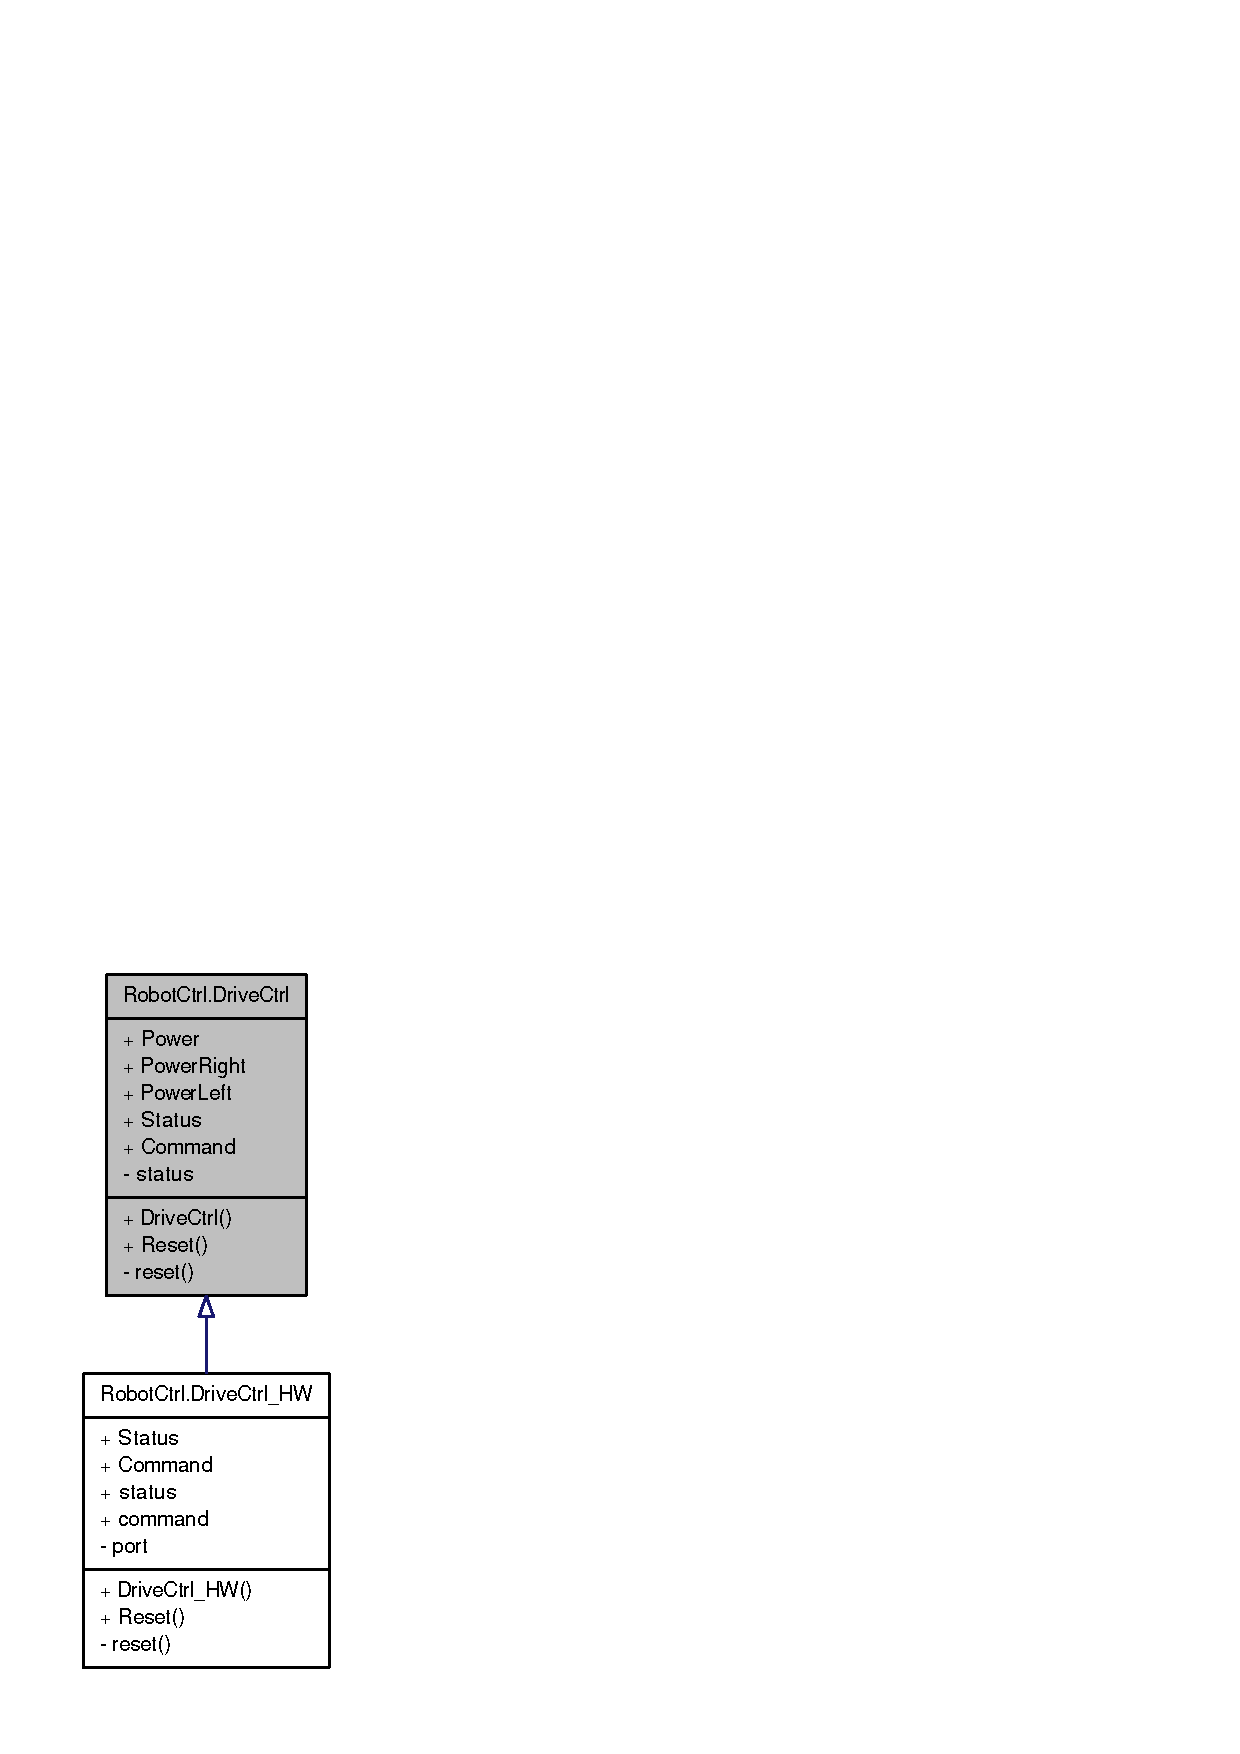
\includegraphics[width=162pt]{class_robot_ctrl_1_1_drive_ctrl__inherit__graph}
\end{center}
\end{figure}
\subsection*{Öffentliche Methoden}
\begin{DoxyCompactItemize}
\item 
\hyperlink{class_robot_ctrl_1_1_drive_ctrl_a8f8e2ebe491712cb323748f7ecc4859a}{DriveCtrl} ()
\item 
virtual void \hyperlink{class_robot_ctrl_1_1_drive_ctrl_a721795047bfe5d2cca3fab6eeb0ab905}{Reset} ()
\end{DoxyCompactItemize}
\subsection*{Propertys}
\begin{DoxyCompactItemize}
\item 
bool \hyperlink{class_robot_ctrl_1_1_drive_ctrl_aef1505229ec4f37b5cc69377360c3f2a}{Power}\hspace{0.3cm}{\ttfamily  \mbox{[}set\mbox{]}}
\item 
bool \hyperlink{class_robot_ctrl_1_1_drive_ctrl_a7fa4a69b83012c16657c9f88a0637754}{PowerRight}\hspace{0.3cm}{\ttfamily  \mbox{[}get, set\mbox{]}}
\item 
bool \hyperlink{class_robot_ctrl_1_1_drive_ctrl_af59bc9fd9c92f7bae49654588693673a}{PowerLeft}\hspace{0.3cm}{\ttfamily  \mbox{[}get, set\mbox{]}}
\item 
virtual int \hyperlink{class_robot_ctrl_1_1_drive_ctrl_a462a4b74b24efb494df863d1ac249b45}{Status}\hspace{0.3cm}{\ttfamily  \mbox{[}get\mbox{]}}
\item 
virtual int \hyperlink{class_robot_ctrl_1_1_drive_ctrl_a45359565bdcb6293ed723acb48cae18b}{Command}\hspace{0.3cm}{\ttfamily  \mbox{[}set\mbox{]}}
\end{DoxyCompactItemize}


\subsection{Ausführliche Beschreibung}
\hyperlink{class_robot_ctrl_1_1_drive_ctrl}{DriveCtrl}, Kommunikation mit der Hardware des Roboters. 

\subsection{Beschreibung der Konstruktoren und Destruktoren}
\hypertarget{class_robot_ctrl_1_1_drive_ctrl_a8f8e2ebe491712cb323748f7ecc4859a}{
\index{RobotCtrl::DriveCtrl@{RobotCtrl::DriveCtrl}!DriveCtrl@{DriveCtrl}}
\index{DriveCtrl@{DriveCtrl}!RobotCtrl::DriveCtrl@{RobotCtrl::DriveCtrl}}
\subsubsection[{DriveCtrl}]{\setlength{\rightskip}{0pt plus 5cm}RobotCtrl.DriveCtrl.DriveCtrl ()}}
\label{class_robot_ctrl_1_1_drive_ctrl_a8f8e2ebe491712cb323748f7ecc4859a}
Standard Konstruktor von \hyperlink{class_robot_ctrl_1_1_drive_ctrl}{DriveCtrl} 

\subsection{Dokumentation der Elementfunktionen}
\hypertarget{class_robot_ctrl_1_1_drive_ctrl_a721795047bfe5d2cca3fab6eeb0ab905}{
\index{RobotCtrl::DriveCtrl@{RobotCtrl::DriveCtrl}!Reset@{Reset}}
\index{Reset@{Reset}!RobotCtrl::DriveCtrl@{RobotCtrl::DriveCtrl}}
\subsubsection[{Reset}]{\setlength{\rightskip}{0pt plus 5cm}virtual void RobotCtrl.DriveCtrl.Reset ()\hspace{0.3cm}{\ttfamily  \mbox{[}virtual\mbox{]}}}}
\label{class_robot_ctrl_1_1_drive_ctrl_a721795047bfe5d2cca3fab6eeb0ab905}
Methode ruft reset() auf. 

Erneute Implementation in \hyperlink{class_robot_ctrl_1_1_drive_ctrl___h_w_a30785a704b5385ea9c41ad87ebb8f61f}{RobotCtrl.DriveCtrl\_\-HW}.



Hier ist ein Graph der zeigt, wo diese Funktion aufgerufen wird:\nopagebreak
\begin{figure}[H]
\begin{center}
\leavevmode
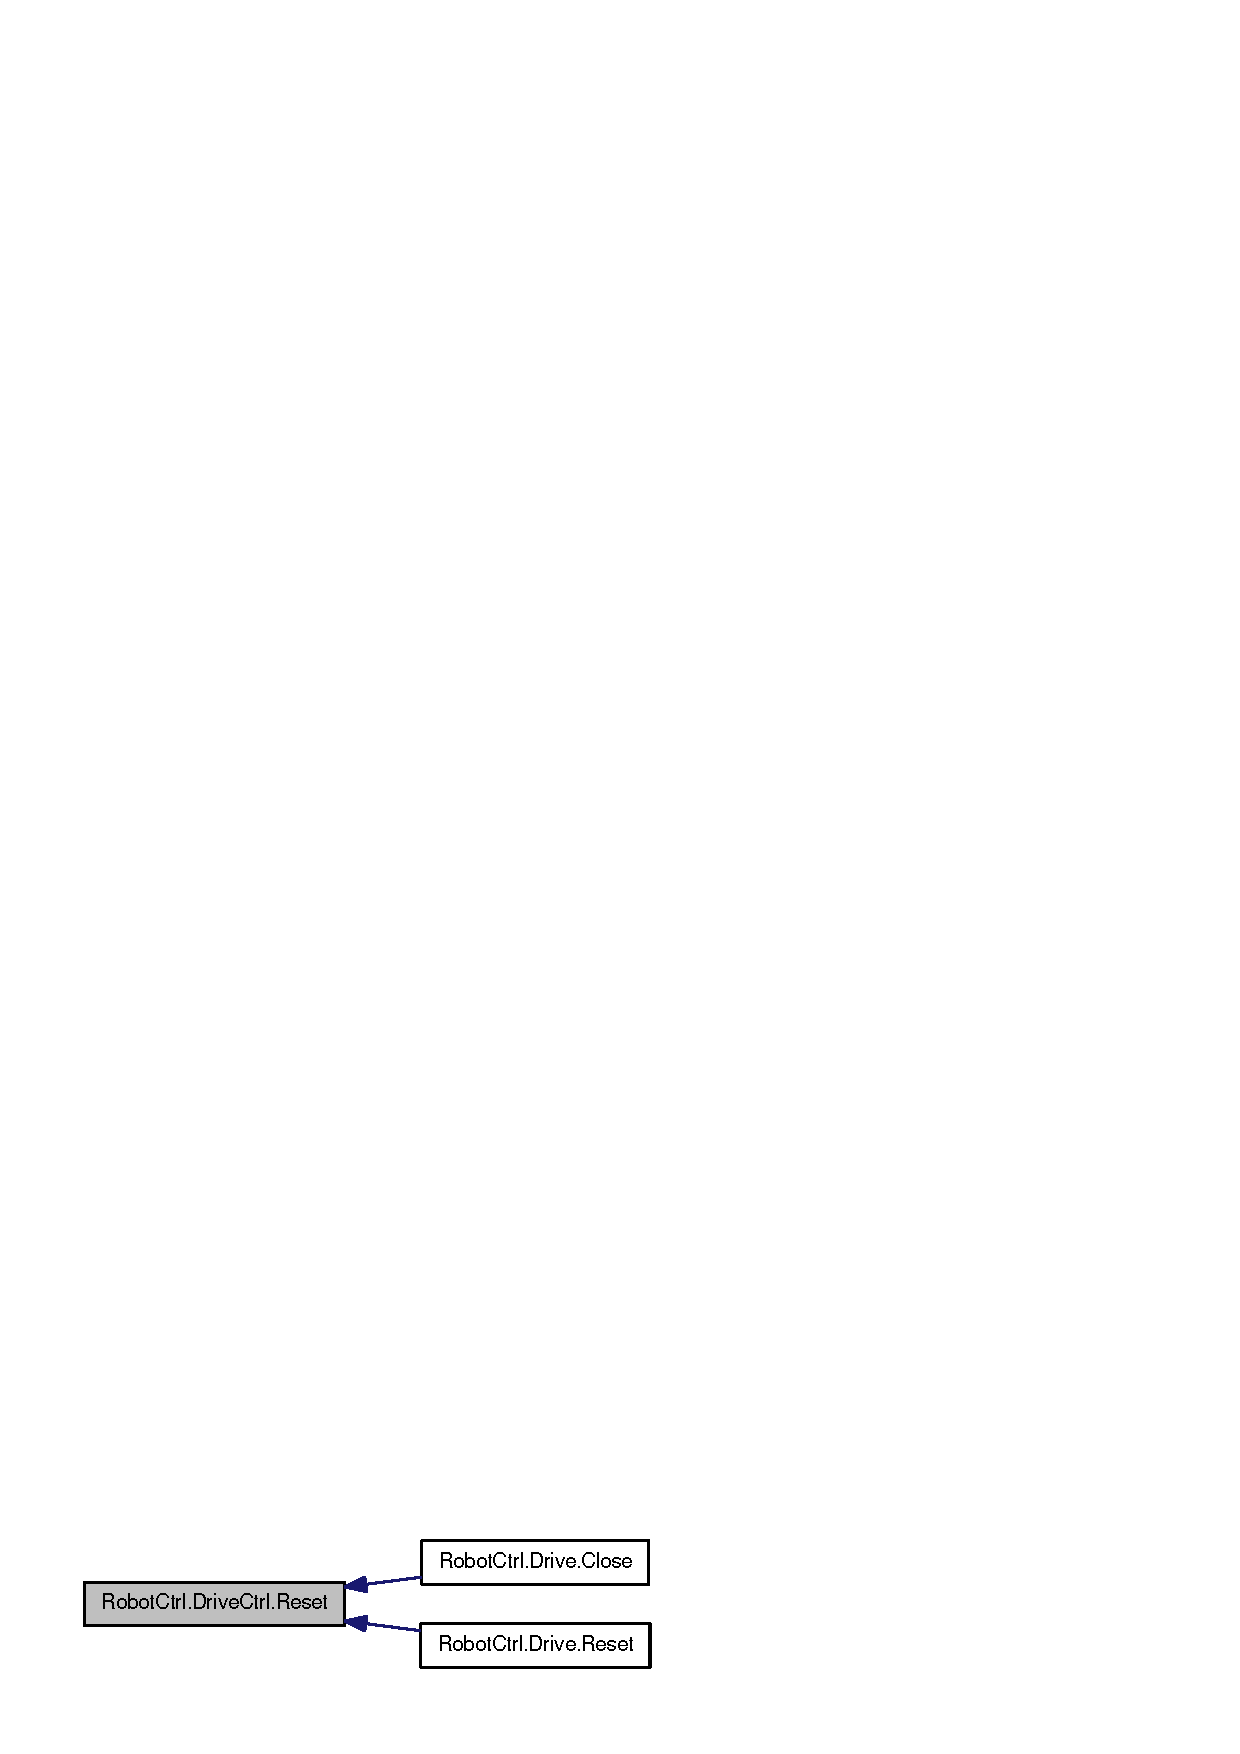
\includegraphics[width=232pt]{class_robot_ctrl_1_1_drive_ctrl_a721795047bfe5d2cca3fab6eeb0ab905_icgraph}
\end{center}
\end{figure}




\subsection{Dokumentation der Propertys}
\hypertarget{class_robot_ctrl_1_1_drive_ctrl_a45359565bdcb6293ed723acb48cae18b}{
\index{RobotCtrl::DriveCtrl@{RobotCtrl::DriveCtrl}!Command@{Command}}
\index{Command@{Command}!RobotCtrl::DriveCtrl@{RobotCtrl::DriveCtrl}}
\subsubsection[{Command}]{\setlength{\rightskip}{0pt plus 5cm}virtual int RobotCtrl.DriveCtrl.Command\hspace{0.3cm}{\ttfamily  \mbox{[}set\mbox{]}}}}
\label{class_robot_ctrl_1_1_drive_ctrl_a45359565bdcb6293ed723acb48cae18b}
Property zum setzen des Status 

Erneute Implementation in \hyperlink{class_robot_ctrl_1_1_drive_ctrl___h_w_acc8cbfa5af4849ee85babc540ad63ada}{RobotCtrl.DriveCtrl\_\-HW}.

\hypertarget{class_robot_ctrl_1_1_drive_ctrl_aef1505229ec4f37b5cc69377360c3f2a}{
\index{RobotCtrl::DriveCtrl@{RobotCtrl::DriveCtrl}!Power@{Power}}
\index{Power@{Power}!RobotCtrl::DriveCtrl@{RobotCtrl::DriveCtrl}}
\subsubsection[{Power}]{\setlength{\rightskip}{0pt plus 5cm}bool RobotCtrl.DriveCtrl.Power\hspace{0.3cm}{\ttfamily  \mbox{[}set\mbox{]}}}}
\label{class_robot_ctrl_1_1_drive_ctrl_aef1505229ec4f37b5cc69377360c3f2a}
Property zum Ein-\/ und Ausschalten der Motoren \hypertarget{class_robot_ctrl_1_1_drive_ctrl_af59bc9fd9c92f7bae49654588693673a}{
\index{RobotCtrl::DriveCtrl@{RobotCtrl::DriveCtrl}!PowerLeft@{PowerLeft}}
\index{PowerLeft@{PowerLeft}!RobotCtrl::DriveCtrl@{RobotCtrl::DriveCtrl}}
\subsubsection[{PowerLeft}]{\setlength{\rightskip}{0pt plus 5cm}bool RobotCtrl.DriveCtrl.PowerLeft\hspace{0.3cm}{\ttfamily  \mbox{[}get, set\mbox{]}}}}
\label{class_robot_ctrl_1_1_drive_ctrl_af59bc9fd9c92f7bae49654588693673a}
Property zum Ein-\/ und Ausschalten des linken Motors \hypertarget{class_robot_ctrl_1_1_drive_ctrl_a7fa4a69b83012c16657c9f88a0637754}{
\index{RobotCtrl::DriveCtrl@{RobotCtrl::DriveCtrl}!PowerRight@{PowerRight}}
\index{PowerRight@{PowerRight}!RobotCtrl::DriveCtrl@{RobotCtrl::DriveCtrl}}
\subsubsection[{PowerRight}]{\setlength{\rightskip}{0pt plus 5cm}bool RobotCtrl.DriveCtrl.PowerRight\hspace{0.3cm}{\ttfamily  \mbox{[}get, set\mbox{]}}}}
\label{class_robot_ctrl_1_1_drive_ctrl_a7fa4a69b83012c16657c9f88a0637754}
Property zum Ein-\/ und Ausschalten des rechten Motors \hypertarget{class_robot_ctrl_1_1_drive_ctrl_a462a4b74b24efb494df863d1ac249b45}{
\index{RobotCtrl::DriveCtrl@{RobotCtrl::DriveCtrl}!Status@{Status}}
\index{Status@{Status}!RobotCtrl::DriveCtrl@{RobotCtrl::DriveCtrl}}
\subsubsection[{Status}]{\setlength{\rightskip}{0pt plus 5cm}virtual int RobotCtrl.DriveCtrl.Status\hspace{0.3cm}{\ttfamily  \mbox{[}get\mbox{]}}}}
\label{class_robot_ctrl_1_1_drive_ctrl_a462a4b74b24efb494df863d1ac249b45}
Property zum auslesen des Status 

Erneute Implementation in \hyperlink{class_robot_ctrl_1_1_drive_ctrl___h_w_ab77cfbe90640881ca1e051fab36f02ac}{RobotCtrl.DriveCtrl\_\-HW}.



Die Dokumentation für diese Klasse wurde erzeugt aufgrund der Datei:\begin{DoxyCompactItemize}
\item 
DriveCtrl.cs\end{DoxyCompactItemize}

\hypertarget{class_robot_ctrl_1_1_drive_ctrl___h_w}{
\section{RobotCtrl.DriveCtrl\_\-HW Klassenreferenz}
\label{class_robot_ctrl_1_1_drive_ctrl___h_w}\index{RobotCtrl::DriveCtrl\_\-HW@{RobotCtrl::DriveCtrl\_\-HW}}
}


Klassendiagramm für RobotCtrl.DriveCtrl\_\-HW:\nopagebreak
\begin{figure}[H]
\begin{center}
\leavevmode
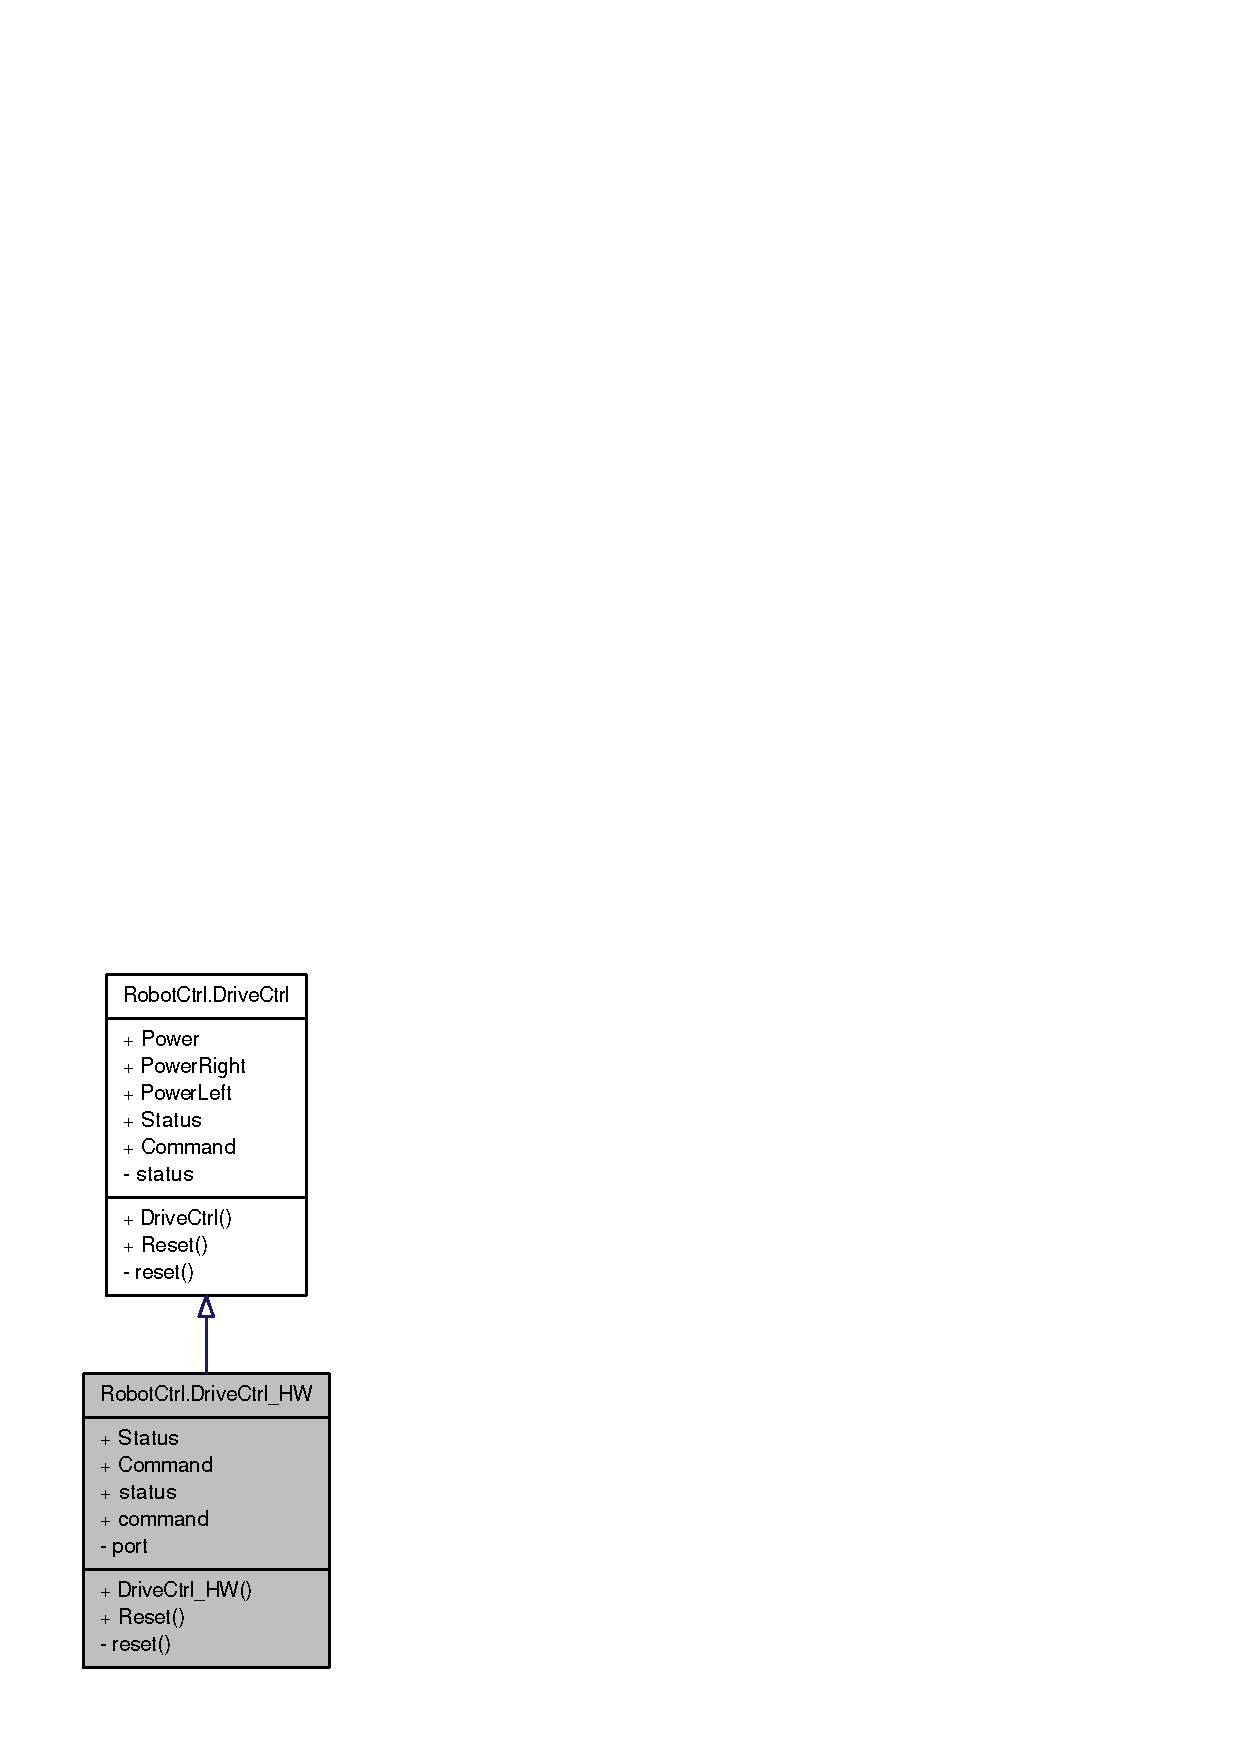
\includegraphics[width=162pt]{class_robot_ctrl_1_1_drive_ctrl___h_w__inherit__graph}
\end{center}
\end{figure}


Zusammengehörigkeiten von RobotCtrl.DriveCtrl\_\-HW:\nopagebreak
\begin{figure}[H]
\begin{center}
\leavevmode
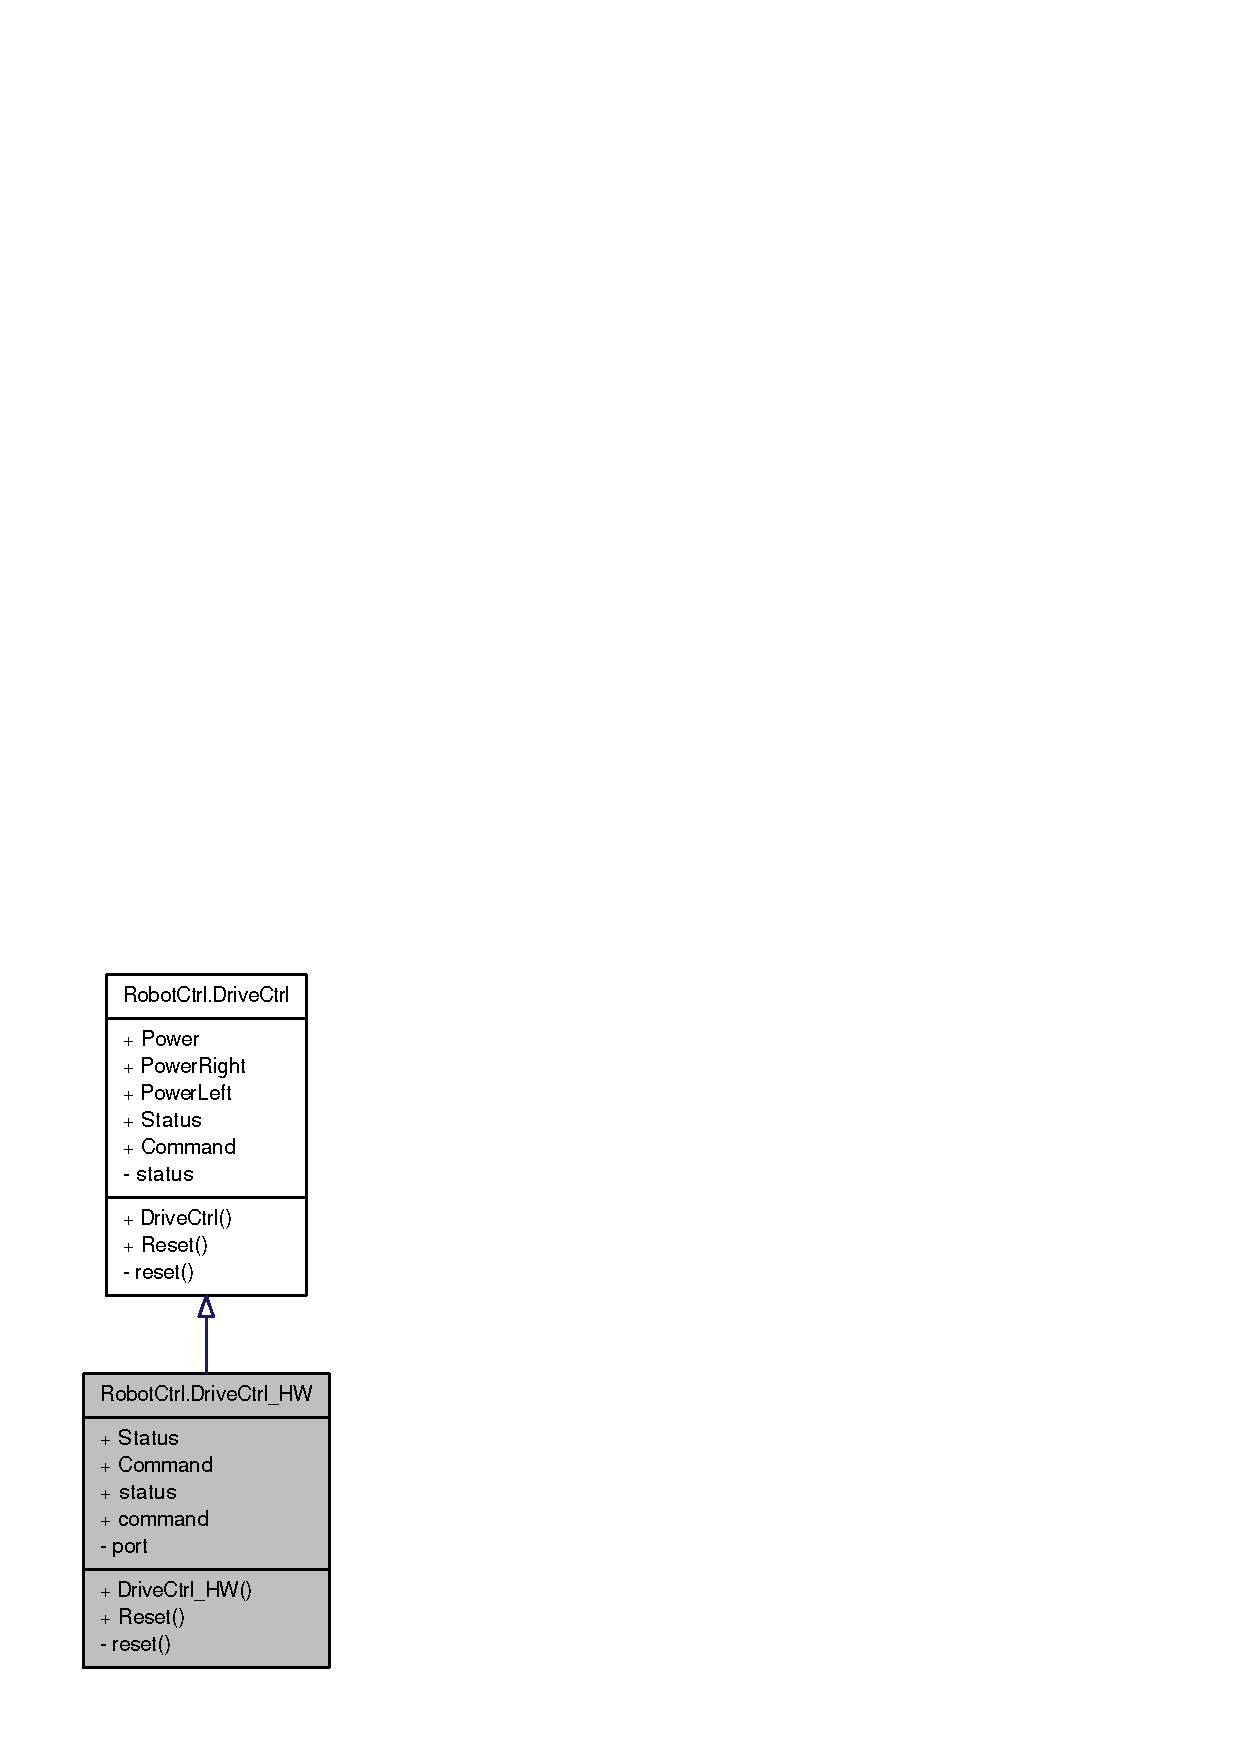
\includegraphics[width=162pt]{class_robot_ctrl_1_1_drive_ctrl___h_w__coll__graph}
\end{center}
\end{figure}
\subsection*{Öffentliche Methoden}
\begin{DoxyCompactItemize}
\item 
\hypertarget{class_robot_ctrl_1_1_drive_ctrl___h_w_a35edb9b280ac1c76f0471ce2204f2235}{
{\bfseries DriveCtrl\_\-HW} (int portAddress)}
\label{class_robot_ctrl_1_1_drive_ctrl___h_w_a35edb9b280ac1c76f0471ce2204f2235}

\item 
\hypertarget{class_robot_ctrl_1_1_drive_ctrl___h_w_a30785a704b5385ea9c41ad87ebb8f61f}{
override void {\bfseries Reset} ()}
\label{class_robot_ctrl_1_1_drive_ctrl___h_w_a30785a704b5385ea9c41ad87ebb8f61f}

\end{DoxyCompactItemize}
\subsection*{Propertys}
\begin{DoxyCompactItemize}
\item 
\hypertarget{class_robot_ctrl_1_1_drive_ctrl___h_w_ab77cfbe90640881ca1e051fab36f02ac}{
override int {\bfseries Status}\hspace{0.3cm}{\ttfamily  \mbox{[}get\mbox{]}}}
\label{class_robot_ctrl_1_1_drive_ctrl___h_w_ab77cfbe90640881ca1e051fab36f02ac}

\item 
\hypertarget{class_robot_ctrl_1_1_drive_ctrl___h_w_acc8cbfa5af4849ee85babc540ad63ada}{
override int {\bfseries Command}\hspace{0.3cm}{\ttfamily  \mbox{[}set\mbox{]}}}
\label{class_robot_ctrl_1_1_drive_ctrl___h_w_acc8cbfa5af4849ee85babc540ad63ada}

\end{DoxyCompactItemize}


Die Dokumentation für diese Klasse wurde erzeugt aufgrund der Datei:\begin{DoxyCompactItemize}
\item 
DriveCtrl\_\-HW.cs\end{DoxyCompactItemize}

\hypertarget{struct_robot_ctrl_1_1_drive_info}{
\section{RobotCtrl.DriveInfo Strukturreferenz}
\label{struct_robot_ctrl_1_1_drive_info}\index{RobotCtrl::DriveInfo@{RobotCtrl::DriveInfo}}
}


Zusammengehörigkeiten von RobotCtrl.DriveInfo:\nopagebreak
\begin{figure}[H]
\begin{center}
\leavevmode
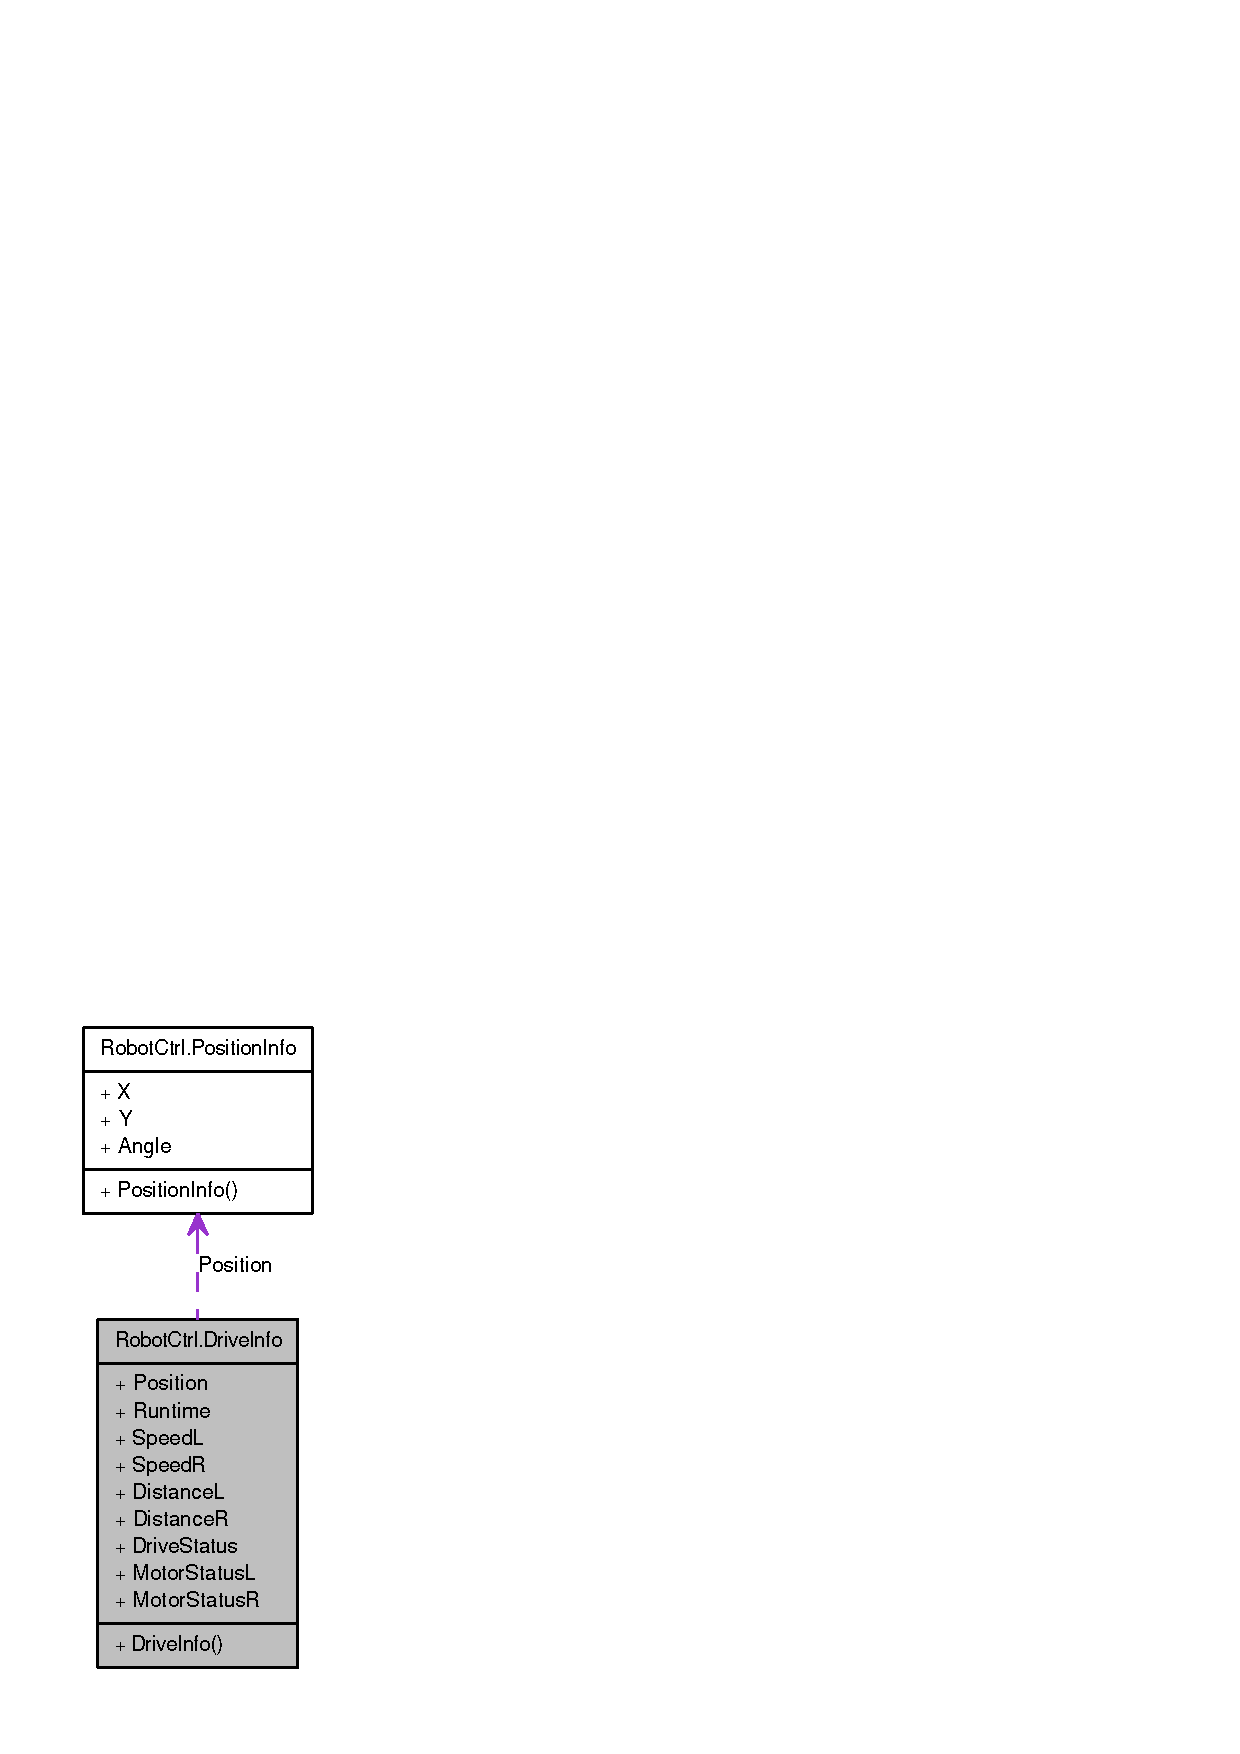
\includegraphics[width=154pt]{struct_robot_ctrl_1_1_drive_info__coll__graph}
\end{center}
\end{figure}
\subsection*{Öffentliche Methoden}
\begin{DoxyCompactItemize}
\item 
\hypertarget{struct_robot_ctrl_1_1_drive_info_a99d9fbb5a1b22a902112898282d68029}{
{\bfseries DriveInfo} (\hyperlink{struct_robot_ctrl_1_1_position_info}{PositionInfo} position, double runtime, double speedL, double speedR, double distanceL, double distanceR, int driveStatus, int motorStatusL, int motorStatusR)}
\label{struct_robot_ctrl_1_1_drive_info_a99d9fbb5a1b22a902112898282d68029}

\end{DoxyCompactItemize}
\subsection*{Öffentliche Attribute}
\begin{DoxyCompactItemize}
\item 
\hypertarget{struct_robot_ctrl_1_1_drive_info_a551f6e86bc5fe62f98dc3a629dc6ed2e}{
\hyperlink{struct_robot_ctrl_1_1_position_info}{PositionInfo} {\bfseries Position}}
\label{struct_robot_ctrl_1_1_drive_info_a551f6e86bc5fe62f98dc3a629dc6ed2e}

\item 
\hypertarget{struct_robot_ctrl_1_1_drive_info_ab7c6391680557d3feaea4432f6d0badf}{
double {\bfseries Runtime}}
\label{struct_robot_ctrl_1_1_drive_info_ab7c6391680557d3feaea4432f6d0badf}

\item 
\hypertarget{struct_robot_ctrl_1_1_drive_info_ab227d6a5642692d88d32adbdb600d97c}{
double {\bfseries SpeedL}}
\label{struct_robot_ctrl_1_1_drive_info_ab227d6a5642692d88d32adbdb600d97c}

\item 
\hypertarget{struct_robot_ctrl_1_1_drive_info_aaeb49b7c4edd218d4df3586aea7f0317}{
double {\bfseries SpeedR}}
\label{struct_robot_ctrl_1_1_drive_info_aaeb49b7c4edd218d4df3586aea7f0317}

\item 
\hypertarget{struct_robot_ctrl_1_1_drive_info_a8927da9def3aa0d9ea8bc1994797bb48}{
double {\bfseries DistanceL}}
\label{struct_robot_ctrl_1_1_drive_info_a8927da9def3aa0d9ea8bc1994797bb48}

\item 
\hypertarget{struct_robot_ctrl_1_1_drive_info_ab83811fd141344442369db7aae6698c7}{
double {\bfseries DistanceR}}
\label{struct_robot_ctrl_1_1_drive_info_ab83811fd141344442369db7aae6698c7}

\item 
\hypertarget{struct_robot_ctrl_1_1_drive_info_af9b93e57cd3ffc06474d39d42a823a6d}{
int {\bfseries DriveStatus}}
\label{struct_robot_ctrl_1_1_drive_info_af9b93e57cd3ffc06474d39d42a823a6d}

\item 
\hypertarget{struct_robot_ctrl_1_1_drive_info_ab13d6cee7fac024d26854348884cfe88}{
int {\bfseries MotorStatusL}}
\label{struct_robot_ctrl_1_1_drive_info_ab13d6cee7fac024d26854348884cfe88}

\item 
\hypertarget{struct_robot_ctrl_1_1_drive_info_aa1c028c3cb8540db78c7ebc30fdb049a}{
int {\bfseries MotorStatusR}}
\label{struct_robot_ctrl_1_1_drive_info_aa1c028c3cb8540db78c7ebc30fdb049a}

\end{DoxyCompactItemize}


Die Dokumentation für diese Struktur wurde erzeugt aufgrund der Datei:\begin{DoxyCompactItemize}
\item 
DriveInfo.cs\end{DoxyCompactItemize}

\hypertarget{class_robot_view_1_1_drive_view}{
\section{RobotView.DriveView Klassenreferenz}
\label{class_robot_view_1_1_drive_view}\index{RobotView::DriveView@{RobotView::DriveView}}
}


Zusammengehörigkeiten von RobotView.DriveView:\nopagebreak
\begin{figure}[H]
\begin{center}
\leavevmode
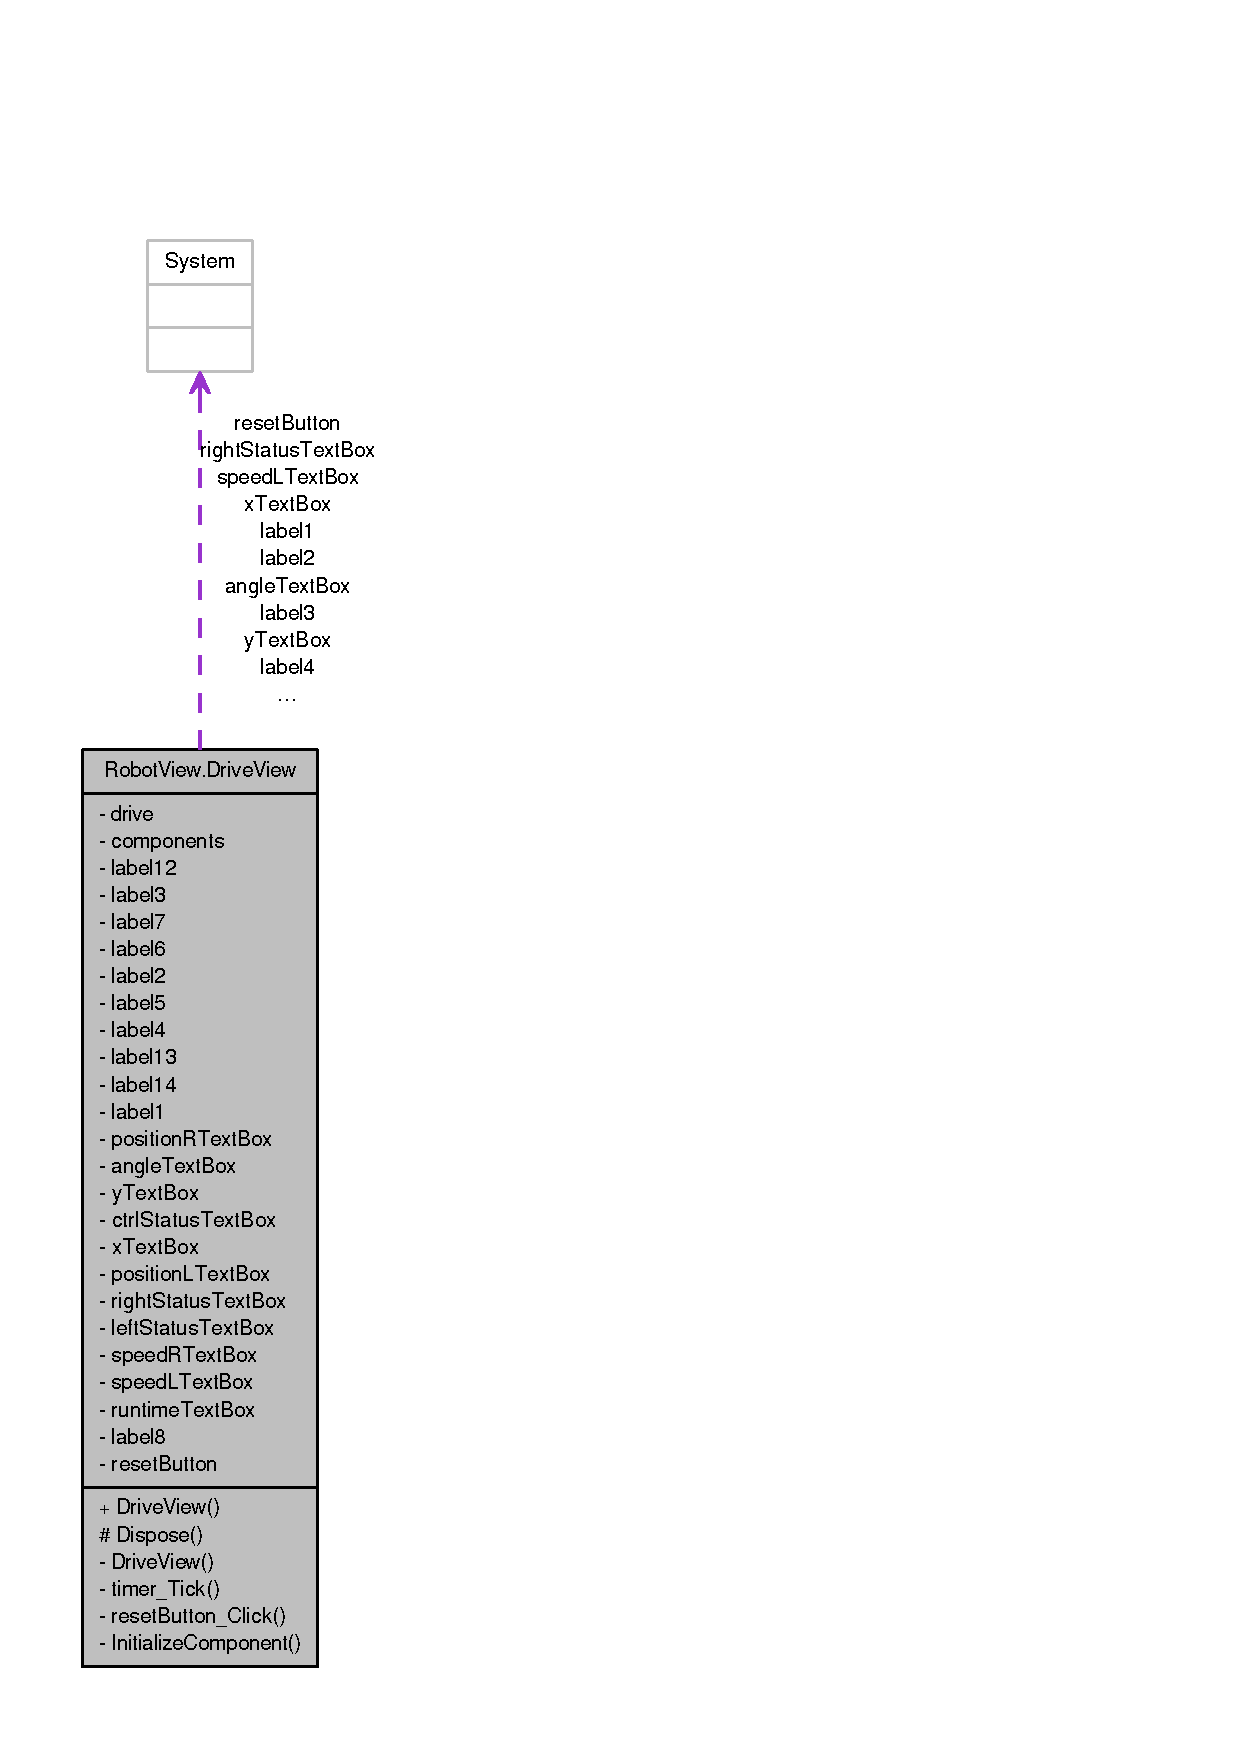
\includegraphics[height=400pt]{class_robot_view_1_1_drive_view__coll__graph}
\end{center}
\end{figure}
\subsection*{Öffentliche Methoden}
\begin{DoxyCompactItemize}
\item 
\hypertarget{class_robot_view_1_1_drive_view_a6f487f04d70fbb0ddaa2f5653d917a1c}{
{\bfseries DriveView} (\hyperlink{class_robot_ctrl_1_1_drive}{Drive} drive)}
\label{class_robot_view_1_1_drive_view_a6f487f04d70fbb0ddaa2f5653d917a1c}

\end{DoxyCompactItemize}
\subsection*{Geschützte Methoden}
\begin{DoxyCompactItemize}
\item 
override void \hyperlink{class_robot_view_1_1_drive_view_a0e75395dfd60b445e558f8071eb08ea5}{Dispose} (bool disposing)
\begin{DoxyCompactList}\small\item\em Clean up any resources being used. \item\end{DoxyCompactList}\end{DoxyCompactItemize}


\subsection{Dokumentation der Elementfunktionen}
\hypertarget{class_robot_view_1_1_drive_view_a0e75395dfd60b445e558f8071eb08ea5}{
\index{RobotView::DriveView@{RobotView::DriveView}!Dispose@{Dispose}}
\index{Dispose@{Dispose}!RobotView::DriveView@{RobotView::DriveView}}
\subsubsection[{Dispose}]{\setlength{\rightskip}{0pt plus 5cm}override void RobotView.DriveView.Dispose (bool {\em disposing})\hspace{0.3cm}{\ttfamily  \mbox{[}protected\mbox{]}}}}
\label{class_robot_view_1_1_drive_view_a0e75395dfd60b445e558f8071eb08ea5}


Clean up any resources being used. 


\begin{DoxyParams}{Parameter}
\item[{\em disposing}]true if managed resources should be disposed; otherwise, false.\end{DoxyParams}


Die Dokumentation für diese Klasse wurde erzeugt aufgrund der Dateien:\begin{DoxyCompactItemize}
\item 
DriveView.cs\item 
DriveView.designer.cs\end{DoxyCompactItemize}

\hypertarget{class_test___console_1_1_form1}{
\section{Test\_\-Console.Form1 Klassenreferenz}
\label{class_test___console_1_1_form1}\index{Test\_\-Console::Form1@{Test\_\-Console::Form1}}
}


Zusammengehörigkeiten von Test\_\-Console.Form1:\nopagebreak
\begin{figure}[H]
\begin{center}
\leavevmode
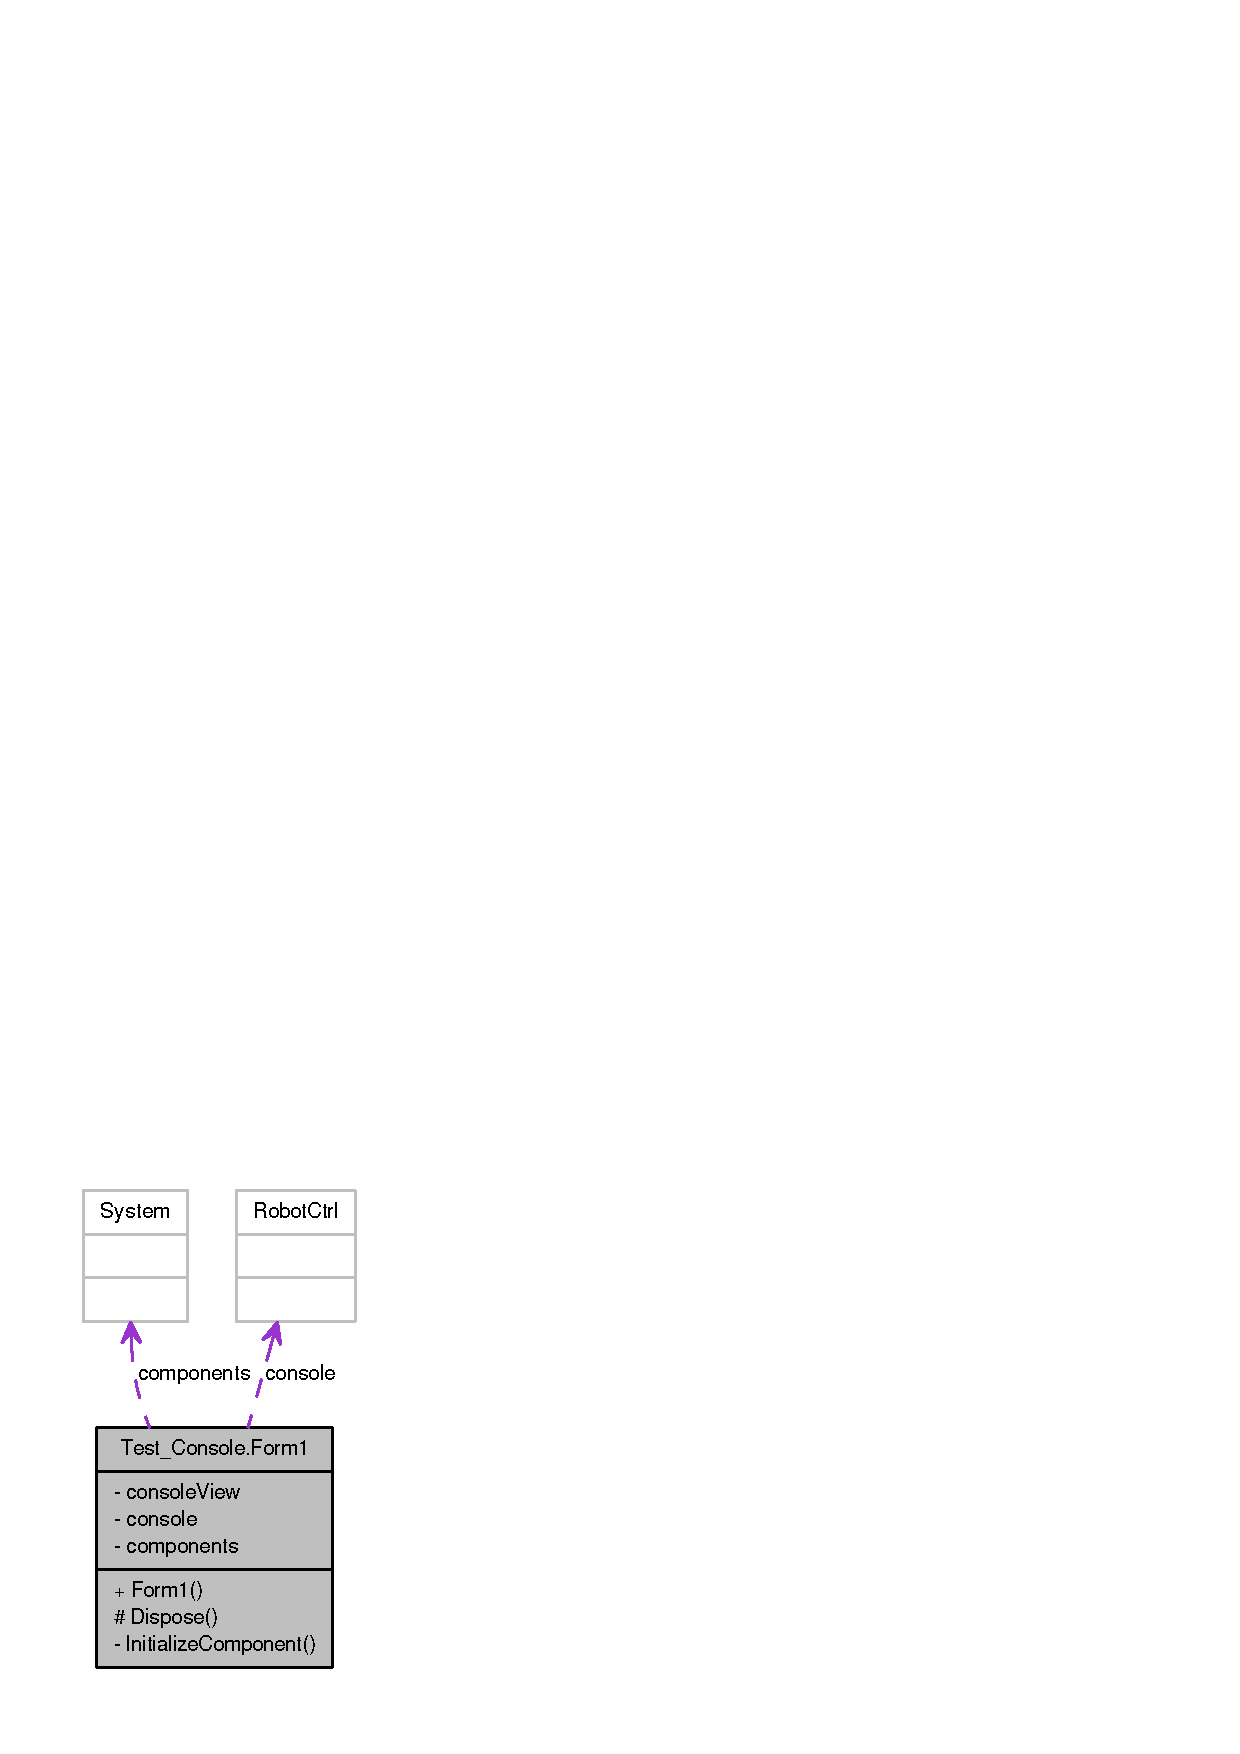
\includegraphics[width=174pt]{class_test___console_1_1_form1__coll__graph}
\end{center}
\end{figure}
\subsection*{Geschützte Methoden}
\begin{DoxyCompactItemize}
\item 
override void \hyperlink{class_test___console_1_1_form1_a7fb762691a68d8aca1928a20ab2ebe77}{Dispose} (bool disposing)
\begin{DoxyCompactList}\small\item\em Verwendete Ressourcen bereinigen. \item\end{DoxyCompactList}\end{DoxyCompactItemize}


\subsection{Dokumentation der Elementfunktionen}
\hypertarget{class_test___console_1_1_form1_a7fb762691a68d8aca1928a20ab2ebe77}{
\index{Test\_\-Console::Form1@{Test\_\-Console::Form1}!Dispose@{Dispose}}
\index{Dispose@{Dispose}!Test_Console::Form1@{Test\_\-Console::Form1}}
\subsubsection[{Dispose}]{\setlength{\rightskip}{0pt plus 5cm}override void Test\_\-Console.Form1.Dispose (bool {\em disposing})\hspace{0.3cm}{\ttfamily  \mbox{[}protected\mbox{]}}}}
\label{class_test___console_1_1_form1_a7fb762691a68d8aca1928a20ab2ebe77}


Verwendete Ressourcen bereinigen. 


\begin{DoxyParams}{Parameter}
\item[{\em disposing}]True, wenn verwaltete Ressourcen gelöscht werden sollen; andernfalls False.\end{DoxyParams}


Die Dokumentation für diese Klasse wurde erzeugt aufgrund der Dateien:\begin{DoxyCompactItemize}
\item 
Test-\/ConsoleForm.cs\item 
Test-\/ConsoleForm.Designer.cs\end{DoxyCompactItemize}

\hypertarget{class_test___lamp_view_1_1_form1}{
\section{Test\_\-LampView.Form1 Klassenreferenz}
\label{class_test___lamp_view_1_1_form1}\index{Test\_\-LampView::Form1@{Test\_\-LampView::Form1}}
}


Zusammengehörigkeiten von Test\_\-LampView.Form1:\nopagebreak
\begin{figure}[H]
\begin{center}
\leavevmode
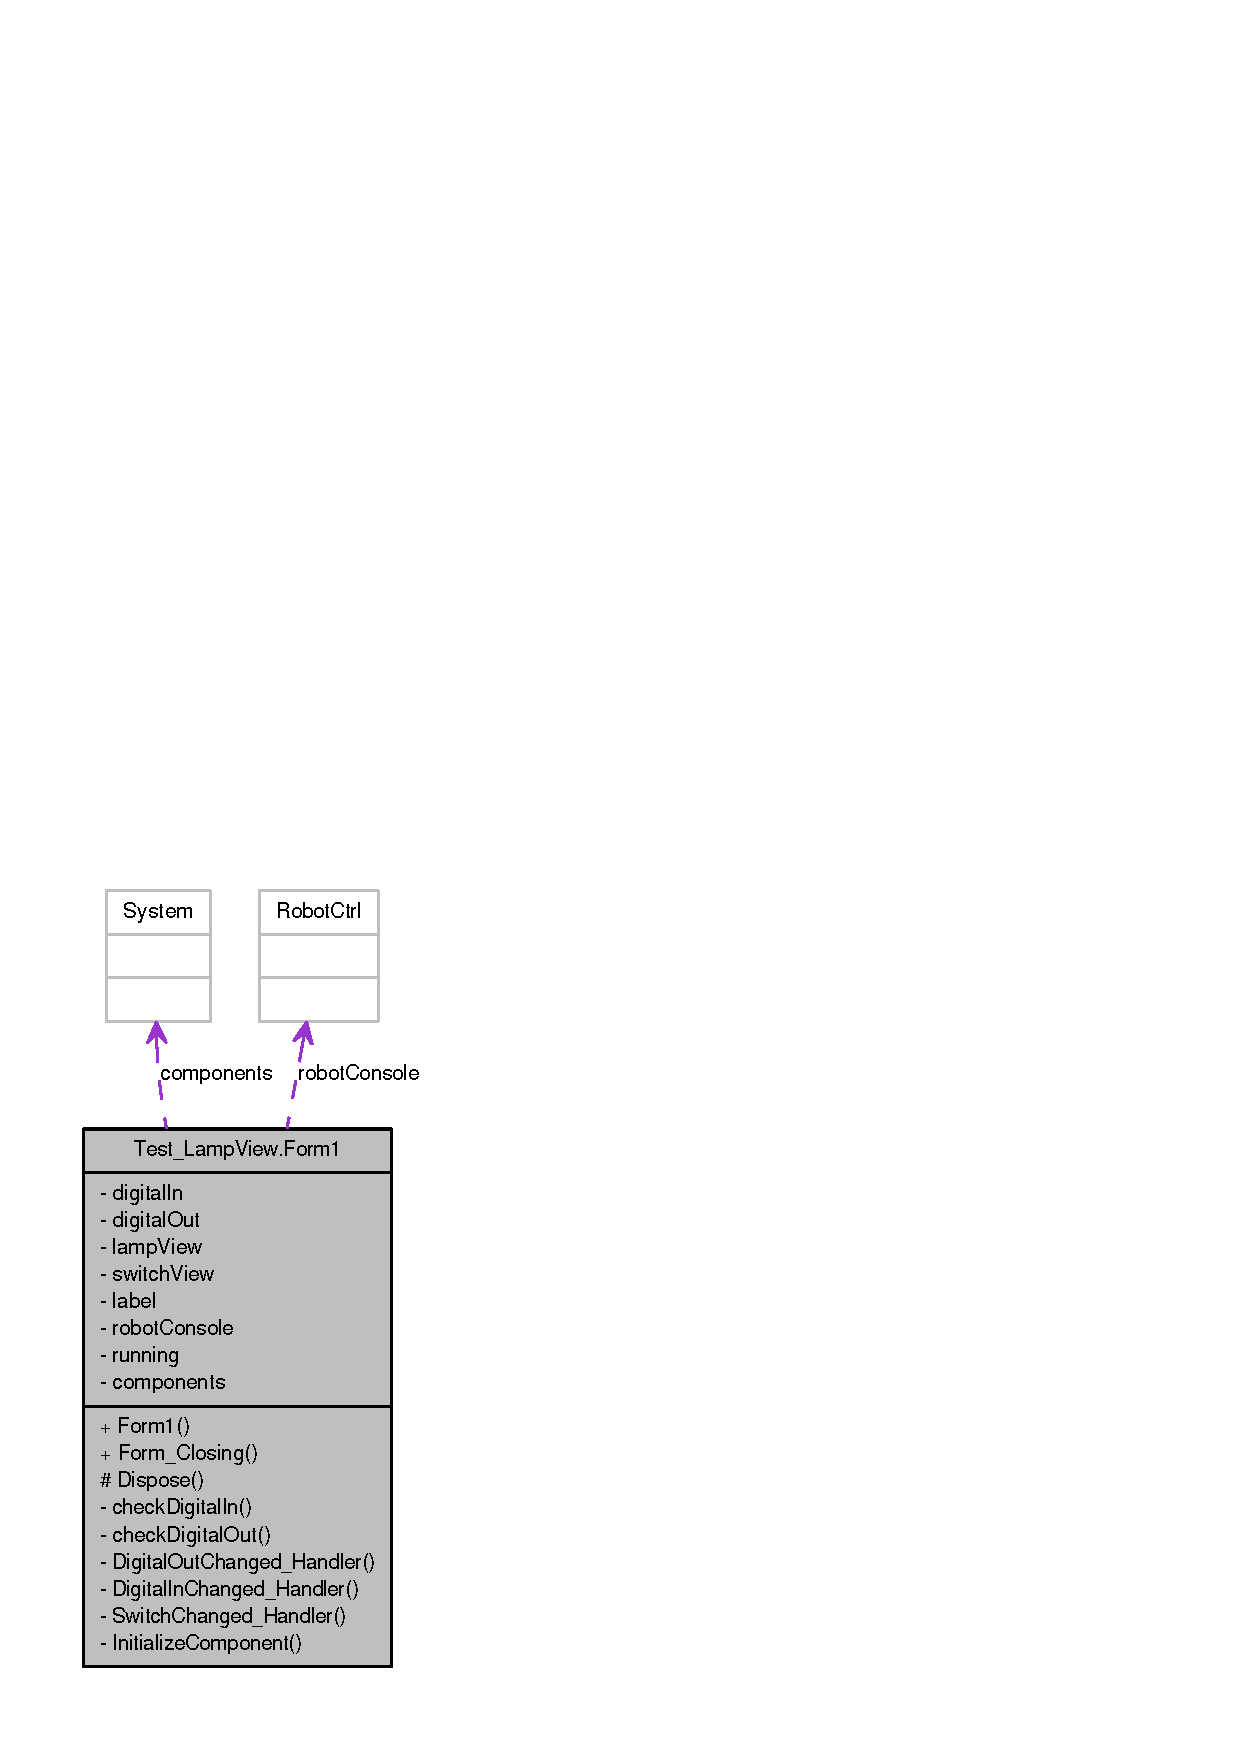
\includegraphics[height=400pt]{class_test___lamp_view_1_1_form1__coll__graph}
\end{center}
\end{figure}
\subsection*{Öffentliche Methoden}
\begin{DoxyCompactItemize}
\item 
\hypertarget{class_test___lamp_view_1_1_form1_ab636f3452c098856ab41a106f7d496d1}{
void {\bfseries Form\_\-Closing} (object sender, CancelEventArgs cArgs)}
\label{class_test___lamp_view_1_1_form1_ab636f3452c098856ab41a106f7d496d1}

\end{DoxyCompactItemize}
\subsection*{Geschützte Methoden}
\begin{DoxyCompactItemize}
\item 
override void \hyperlink{class_test___lamp_view_1_1_form1_a450d572ace13815beff4ac88c22c8d6c}{Dispose} (bool disposing)
\begin{DoxyCompactList}\small\item\em Verwendete Ressourcen bereinigen. \item\end{DoxyCompactList}\end{DoxyCompactItemize}
\subsection*{Ereignisse}
\begin{DoxyCompactItemize}
\item 
\hypertarget{class_test___lamp_view_1_1_form1_a8a2400bdd066b2b481cee52a9b0e2893}{
System.EventHandler {\bfseries DigitalInChanged}}
\label{class_test___lamp_view_1_1_form1_a8a2400bdd066b2b481cee52a9b0e2893}

\item 
\hypertarget{class_test___lamp_view_1_1_form1_a78e050394675cf1d7c55f80243eaae03}{
System.EventHandler {\bfseries DigitalOutChanged}}
\label{class_test___lamp_view_1_1_form1_a78e050394675cf1d7c55f80243eaae03}

\end{DoxyCompactItemize}


\subsection{Dokumentation der Elementfunktionen}
\hypertarget{class_test___lamp_view_1_1_form1_a450d572ace13815beff4ac88c22c8d6c}{
\index{Test\_\-LampView::Form1@{Test\_\-LampView::Form1}!Dispose@{Dispose}}
\index{Dispose@{Dispose}!Test_LampView::Form1@{Test\_\-LampView::Form1}}
\subsubsection[{Dispose}]{\setlength{\rightskip}{0pt plus 5cm}override void Test\_\-LampView.Form1.Dispose (bool {\em disposing})\hspace{0.3cm}{\ttfamily  \mbox{[}protected\mbox{]}}}}
\label{class_test___lamp_view_1_1_form1_a450d572ace13815beff4ac88c22c8d6c}


Verwendete Ressourcen bereinigen. 


\begin{DoxyParams}{Parameter}
\item[{\em disposing}]True, wenn verwaltete Ressourcen gelöscht werden sollen; andernfalls False.\end{DoxyParams}


Die Dokumentation für diese Klasse wurde erzeugt aufgrund der Dateien:\begin{DoxyCompactItemize}
\item 
Test-\/LampView/Form1.cs\item 
Test-\/LampView/Form1.Designer.cs\end{DoxyCompactItemize}

\hypertarget{class_drive_test_1_1_form1}{
\section{DriveTest.Form1 Klassenreferenz}
\label{class_drive_test_1_1_form1}\index{DriveTest::Form1@{DriveTest::Form1}}
}


Zusammengehörigkeiten von DriveTest.Form1:\nopagebreak
\begin{figure}[H]
\begin{center}
\leavevmode
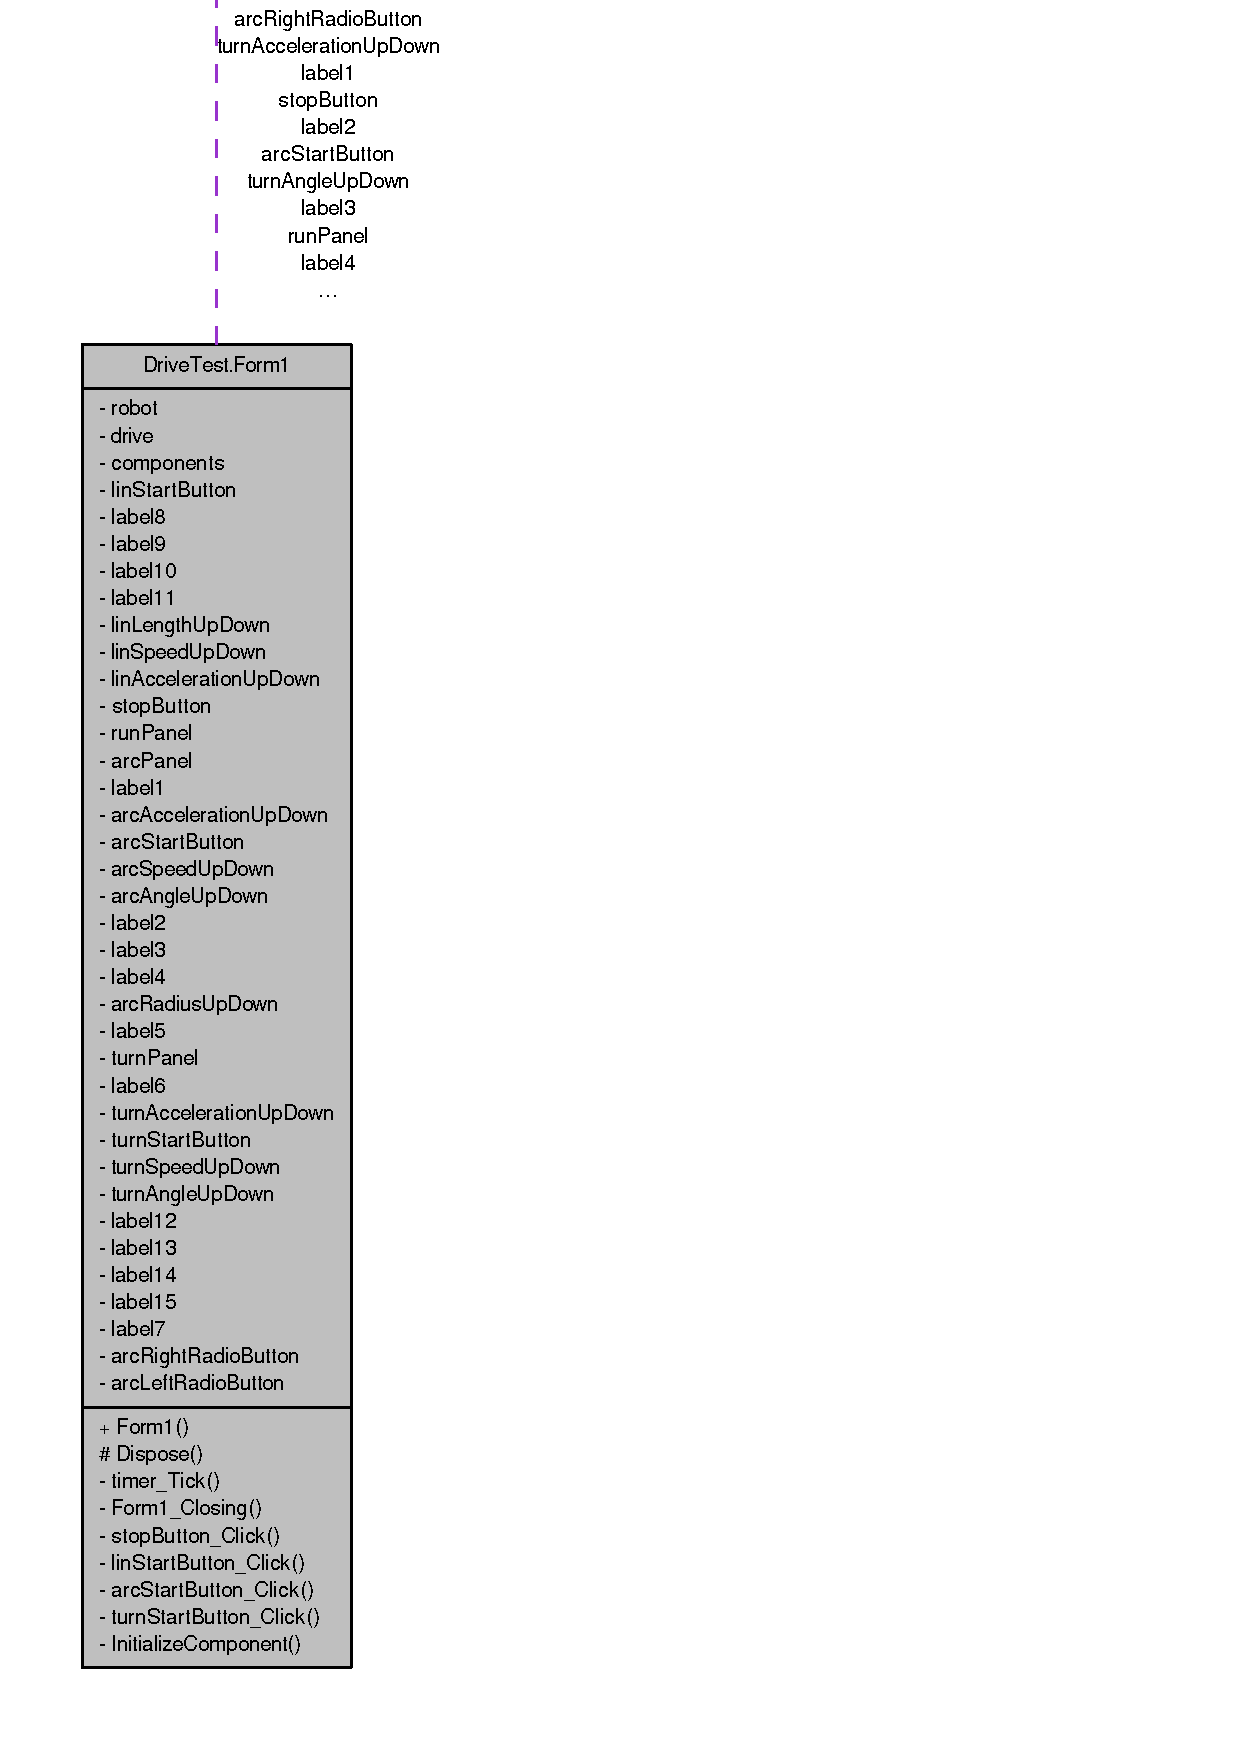
\includegraphics[height=400pt]{class_drive_test_1_1_form1__coll__graph}
\end{center}
\end{figure}
\subsection*{Geschützte Methoden}
\begin{DoxyCompactItemize}
\item 
override void \hyperlink{class_drive_test_1_1_form1_a214a0a440a31be16cf29a0d717bfa824}{Dispose} (bool disposing)
\begin{DoxyCompactList}\small\item\em Verwendete Ressourcen bereinigen. \item\end{DoxyCompactList}\end{DoxyCompactItemize}


\subsection{Dokumentation der Elementfunktionen}
\hypertarget{class_drive_test_1_1_form1_a214a0a440a31be16cf29a0d717bfa824}{
\index{DriveTest::Form1@{DriveTest::Form1}!Dispose@{Dispose}}
\index{Dispose@{Dispose}!DriveTest::Form1@{DriveTest::Form1}}
\subsubsection[{Dispose}]{\setlength{\rightskip}{0pt plus 5cm}override void DriveTest.Form1.Dispose (bool {\em disposing})\hspace{0.3cm}{\ttfamily  \mbox{[}protected\mbox{]}}}}
\label{class_drive_test_1_1_form1_a214a0a440a31be16cf29a0d717bfa824}


Verwendete Ressourcen bereinigen. 


\begin{DoxyParams}{Parameter}
\item[{\em disposing}]True, wenn verwaltete Ressourcen gelöscht werden sollen; andernfalls False.\end{DoxyParams}


Die Dokumentation für diese Klasse wurde erzeugt aufgrund der Dateien:\begin{DoxyCompactItemize}
\item 
Test\_\-Drive\_\-CE/Form1.cs\item 
Test\_\-Drive\_\-CE/Form1.Designer.cs\end{DoxyCompactItemize}

\hypertarget{class_motor_test_1_1_form1}{
\section{MotorTest.Form1 Klassenreferenz}
\label{class_motor_test_1_1_form1}\index{MotorTest::Form1@{MotorTest::Form1}}
}


Zusammengehörigkeiten von MotorTest.Form1:\nopagebreak
\begin{figure}[H]
\begin{center}
\leavevmode
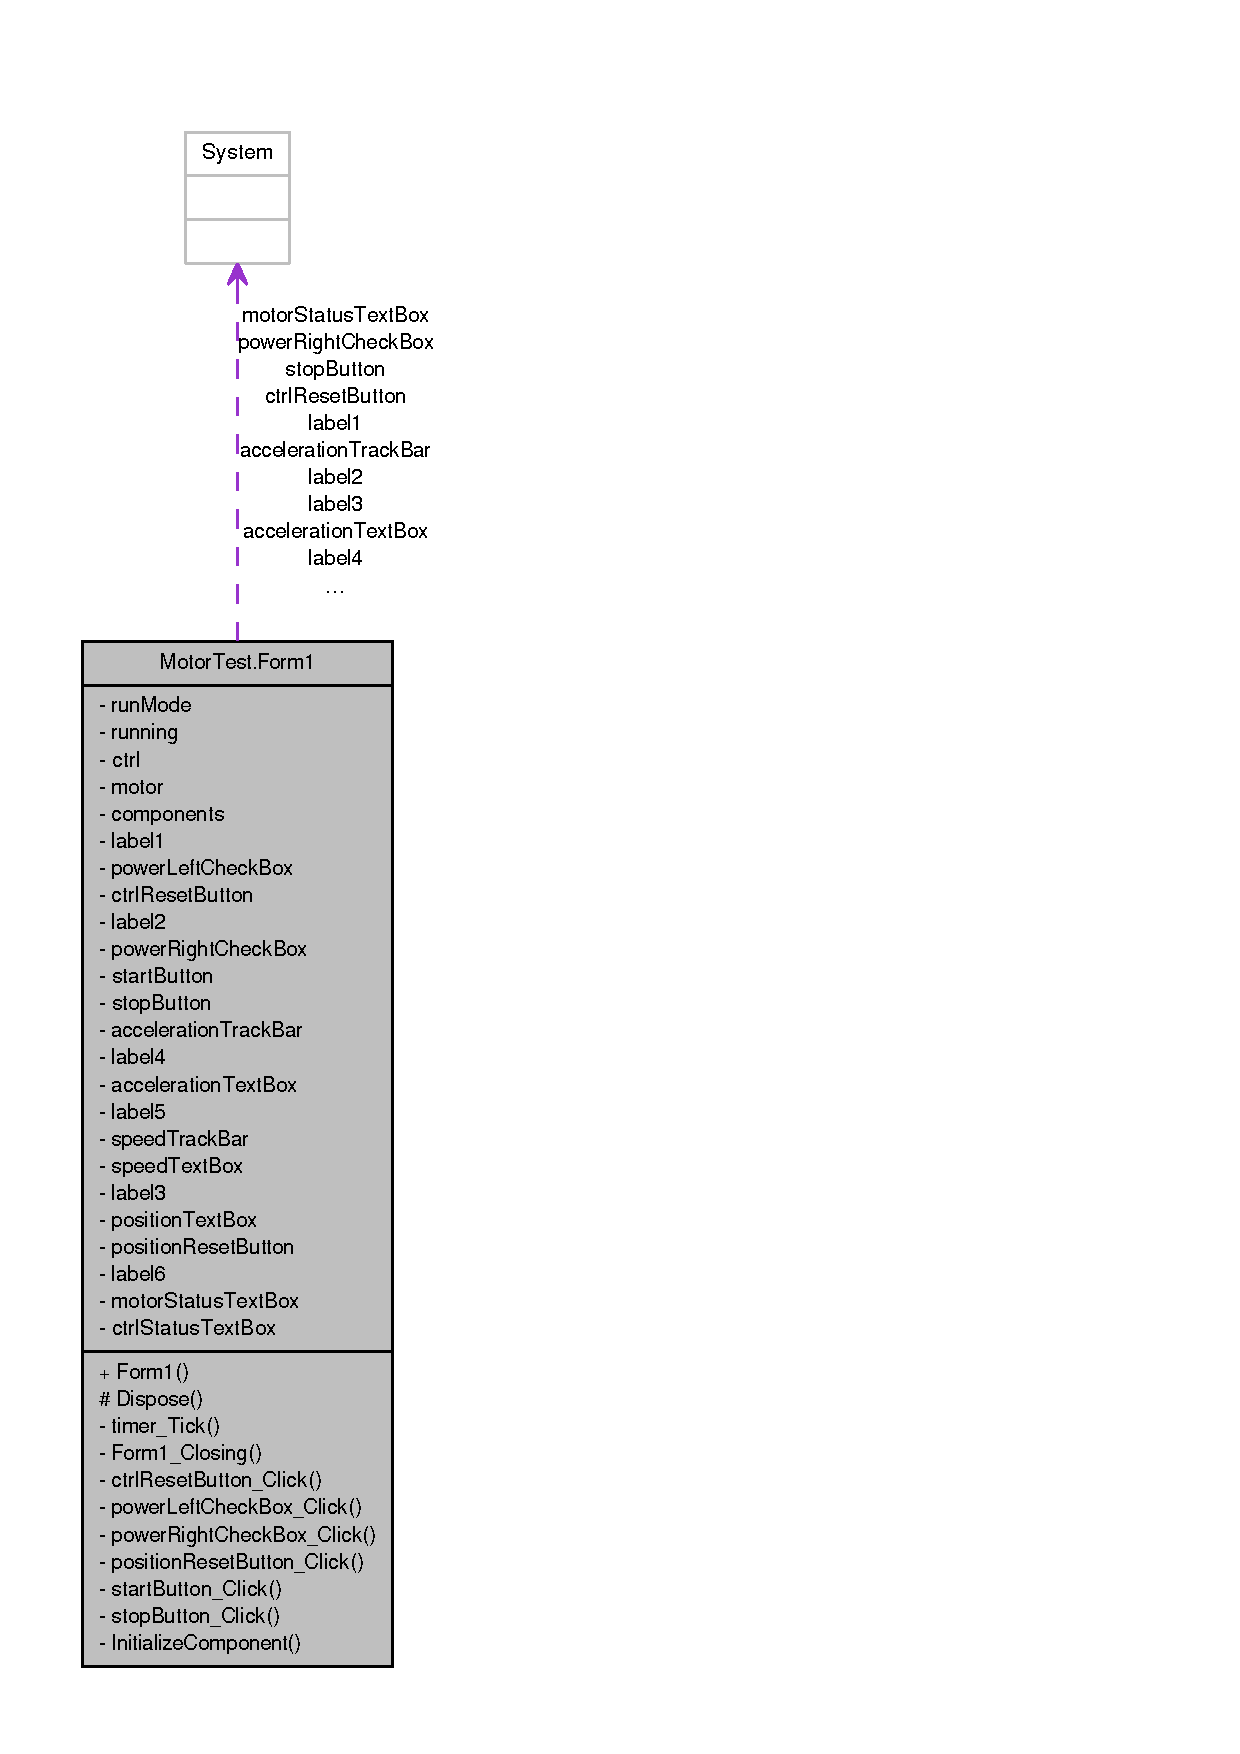
\includegraphics[height=400pt]{class_motor_test_1_1_form1__coll__graph}
\end{center}
\end{figure}
\subsection*{Geschützte Methoden}
\begin{DoxyCompactItemize}
\item 
override void \hyperlink{class_motor_test_1_1_form1_ac013ea3d053663a5aa419e04c31e5273}{Dispose} (bool disposing)
\begin{DoxyCompactList}\small\item\em Clean up any resources being used. \item\end{DoxyCompactList}\end{DoxyCompactItemize}


\subsection{Dokumentation der Elementfunktionen}
\hypertarget{class_motor_test_1_1_form1_ac013ea3d053663a5aa419e04c31e5273}{
\index{MotorTest::Form1@{MotorTest::Form1}!Dispose@{Dispose}}
\index{Dispose@{Dispose}!MotorTest::Form1@{MotorTest::Form1}}
\subsubsection[{Dispose}]{\setlength{\rightskip}{0pt plus 5cm}override void MotorTest.Form1.Dispose (bool {\em disposing})\hspace{0.3cm}{\ttfamily  \mbox{[}protected\mbox{]}}}}
\label{class_motor_test_1_1_form1_ac013ea3d053663a5aa419e04c31e5273}


Clean up any resources being used. 


\begin{DoxyParams}{Parameter}
\item[{\em disposing}]true if managed resources should be disposed; otherwise, false.\end{DoxyParams}


Die Dokumentation für diese Klasse wurde erzeugt aufgrund der Dateien:\begin{DoxyCompactItemize}
\item 
Test\_\-Motor\_\-CE/Form1.cs\item 
Test\_\-Motor\_\-CE/Form1.Designer.cs\end{DoxyCompactItemize}

\hypertarget{class_test___world_1_1_form1}{
\section{Test\_\-World.Form1 Klassenreferenz}
\label{class_test___world_1_1_form1}\index{Test\_\-World::Form1@{Test\_\-World::Form1}}
}


Zusammengehörigkeiten von Test\_\-World.Form1:\nopagebreak
\begin{figure}[H]
\begin{center}
\leavevmode
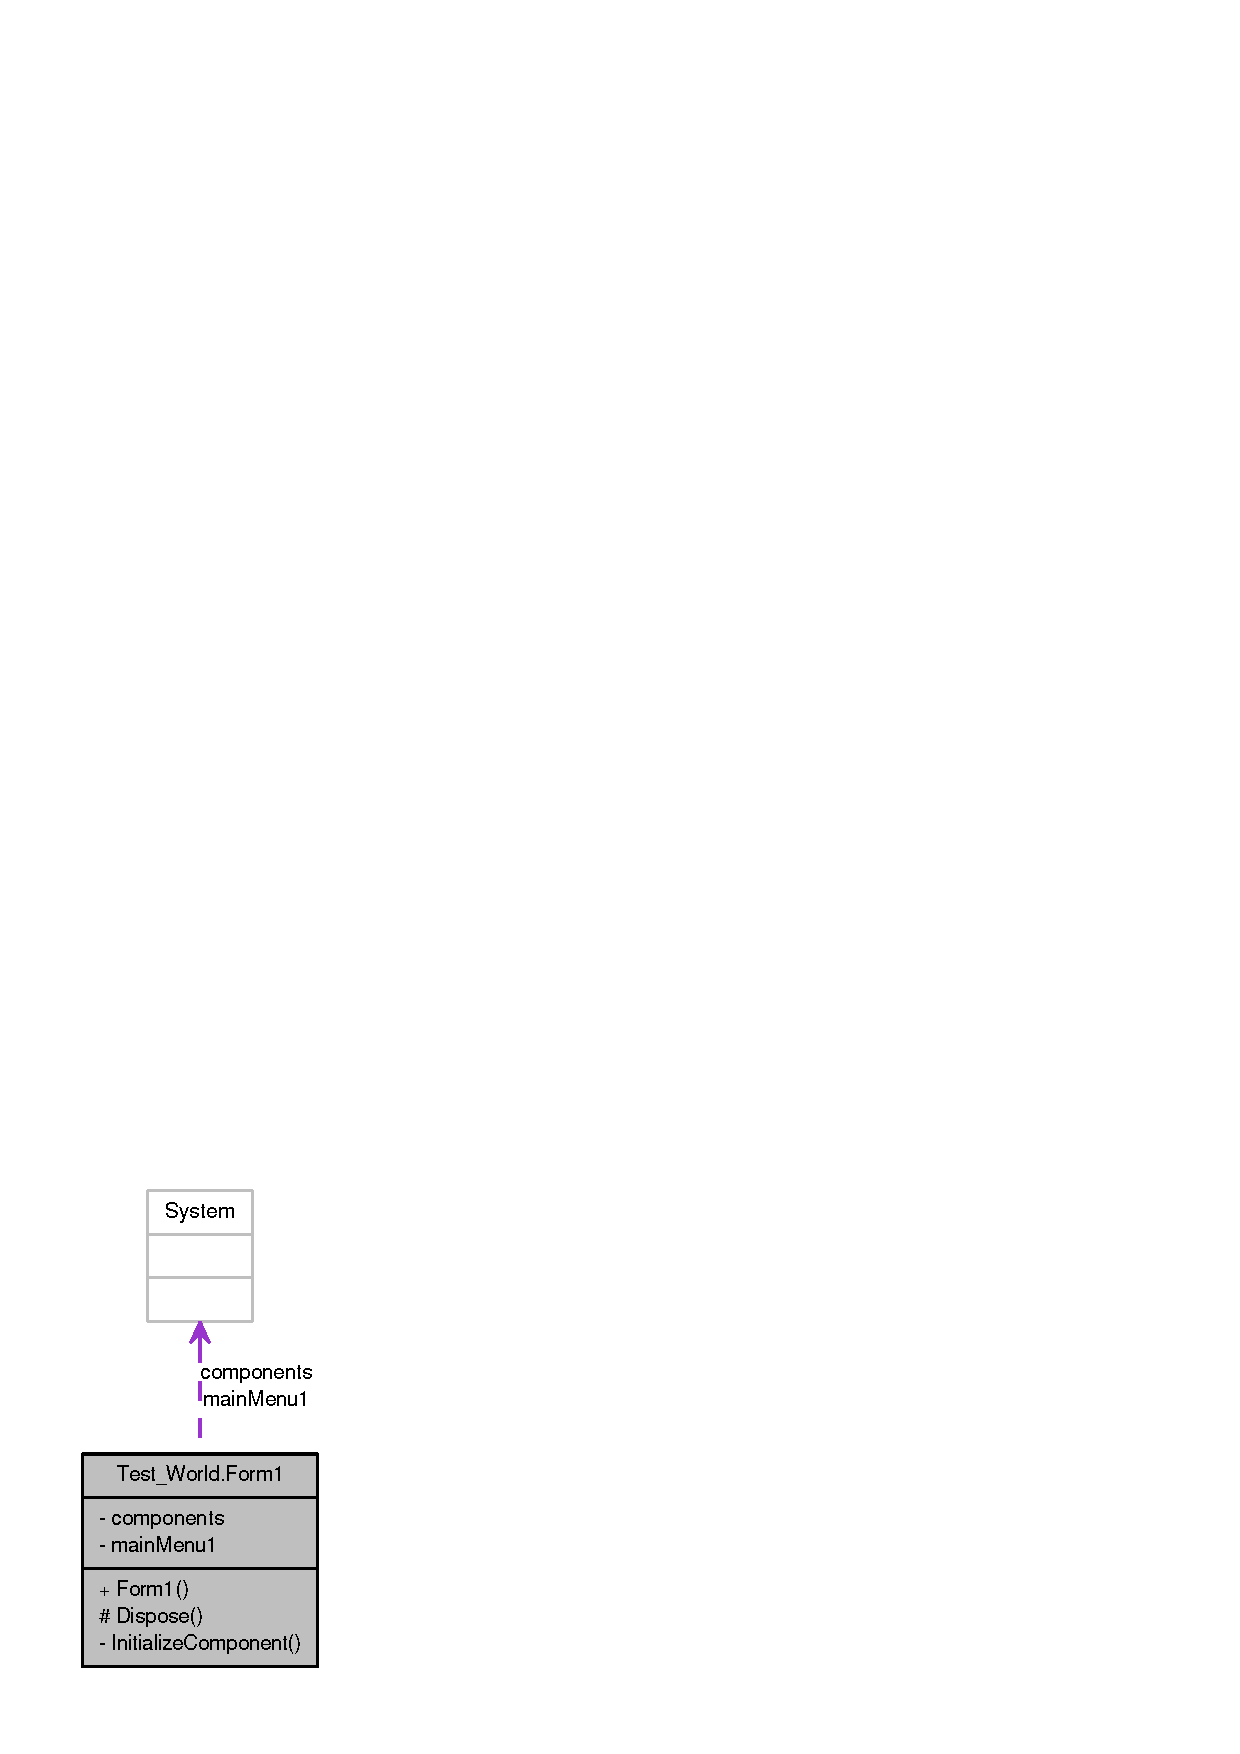
\includegraphics[width=156pt]{class_test___world_1_1_form1__coll__graph}
\end{center}
\end{figure}
\subsection*{Geschützte Methoden}
\begin{DoxyCompactItemize}
\item 
override void \hyperlink{class_test___world_1_1_form1_a76e28105467035fd345da22985304e4b}{Dispose} (bool disposing)
\begin{DoxyCompactList}\small\item\em Verwendete Ressourcen bereinigen. \item\end{DoxyCompactList}\end{DoxyCompactItemize}


\subsection{Dokumentation der Elementfunktionen}
\hypertarget{class_test___world_1_1_form1_a76e28105467035fd345da22985304e4b}{
\index{Test\_\-World::Form1@{Test\_\-World::Form1}!Dispose@{Dispose}}
\index{Dispose@{Dispose}!Test_World::Form1@{Test\_\-World::Form1}}
\subsubsection[{Dispose}]{\setlength{\rightskip}{0pt plus 5cm}override void Test\_\-World.Form1.Dispose (bool {\em disposing})\hspace{0.3cm}{\ttfamily  \mbox{[}protected\mbox{]}}}}
\label{class_test___world_1_1_form1_a76e28105467035fd345da22985304e4b}


Verwendete Ressourcen bereinigen. 


\begin{DoxyParams}{Parameter}
\item[{\em disposing}]True, wenn verwaltete Ressourcen gelöscht werden sollen; andernfalls False.\end{DoxyParams}


Die Dokumentation für diese Klasse wurde erzeugt aufgrund der Dateien:\begin{DoxyCompactItemize}
\item 
Test\_\-World/Form1.cs\item 
Test\_\-World/Form1.Designer.cs\end{DoxyCompactItemize}

\hypertarget{class_robot_view_1_1_lamp_view}{
\section{RobotView.LampView Klassenreferenz}
\label{class_robot_view_1_1_lamp_view}\index{RobotView::LampView@{RobotView::LampView}}
}
\subsection*{Propertys}
\begin{DoxyCompactItemize}
\item 
\hypertarget{class_robot_view_1_1_lamp_view_a30573da6542638c876da84f80bdcaeac}{
bool {\bfseries State}\hspace{0.3cm}{\ttfamily  \mbox{[}get, set\mbox{]}}}
\label{class_robot_view_1_1_lamp_view_a30573da6542638c876da84f80bdcaeac}

\end{DoxyCompactItemize}


Die Dokumentation für diese Klasse wurde erzeugt aufgrund der Datei:\begin{DoxyCompactItemize}
\item 
LampView.cs\end{DoxyCompactItemize}

\hypertarget{class_robot_ctrl_1_1_motor_ctrl}{
\section{RobotCtrl.MotorCtrl Klassenreferenz}
\label{class_robot_ctrl_1_1_motor_ctrl}\index{RobotCtrl::MotorCtrl@{RobotCtrl::MotorCtrl}}
}


Klassendiagramm für RobotCtrl.MotorCtrl:\nopagebreak
\begin{figure}[H]
\begin{center}
\leavevmode
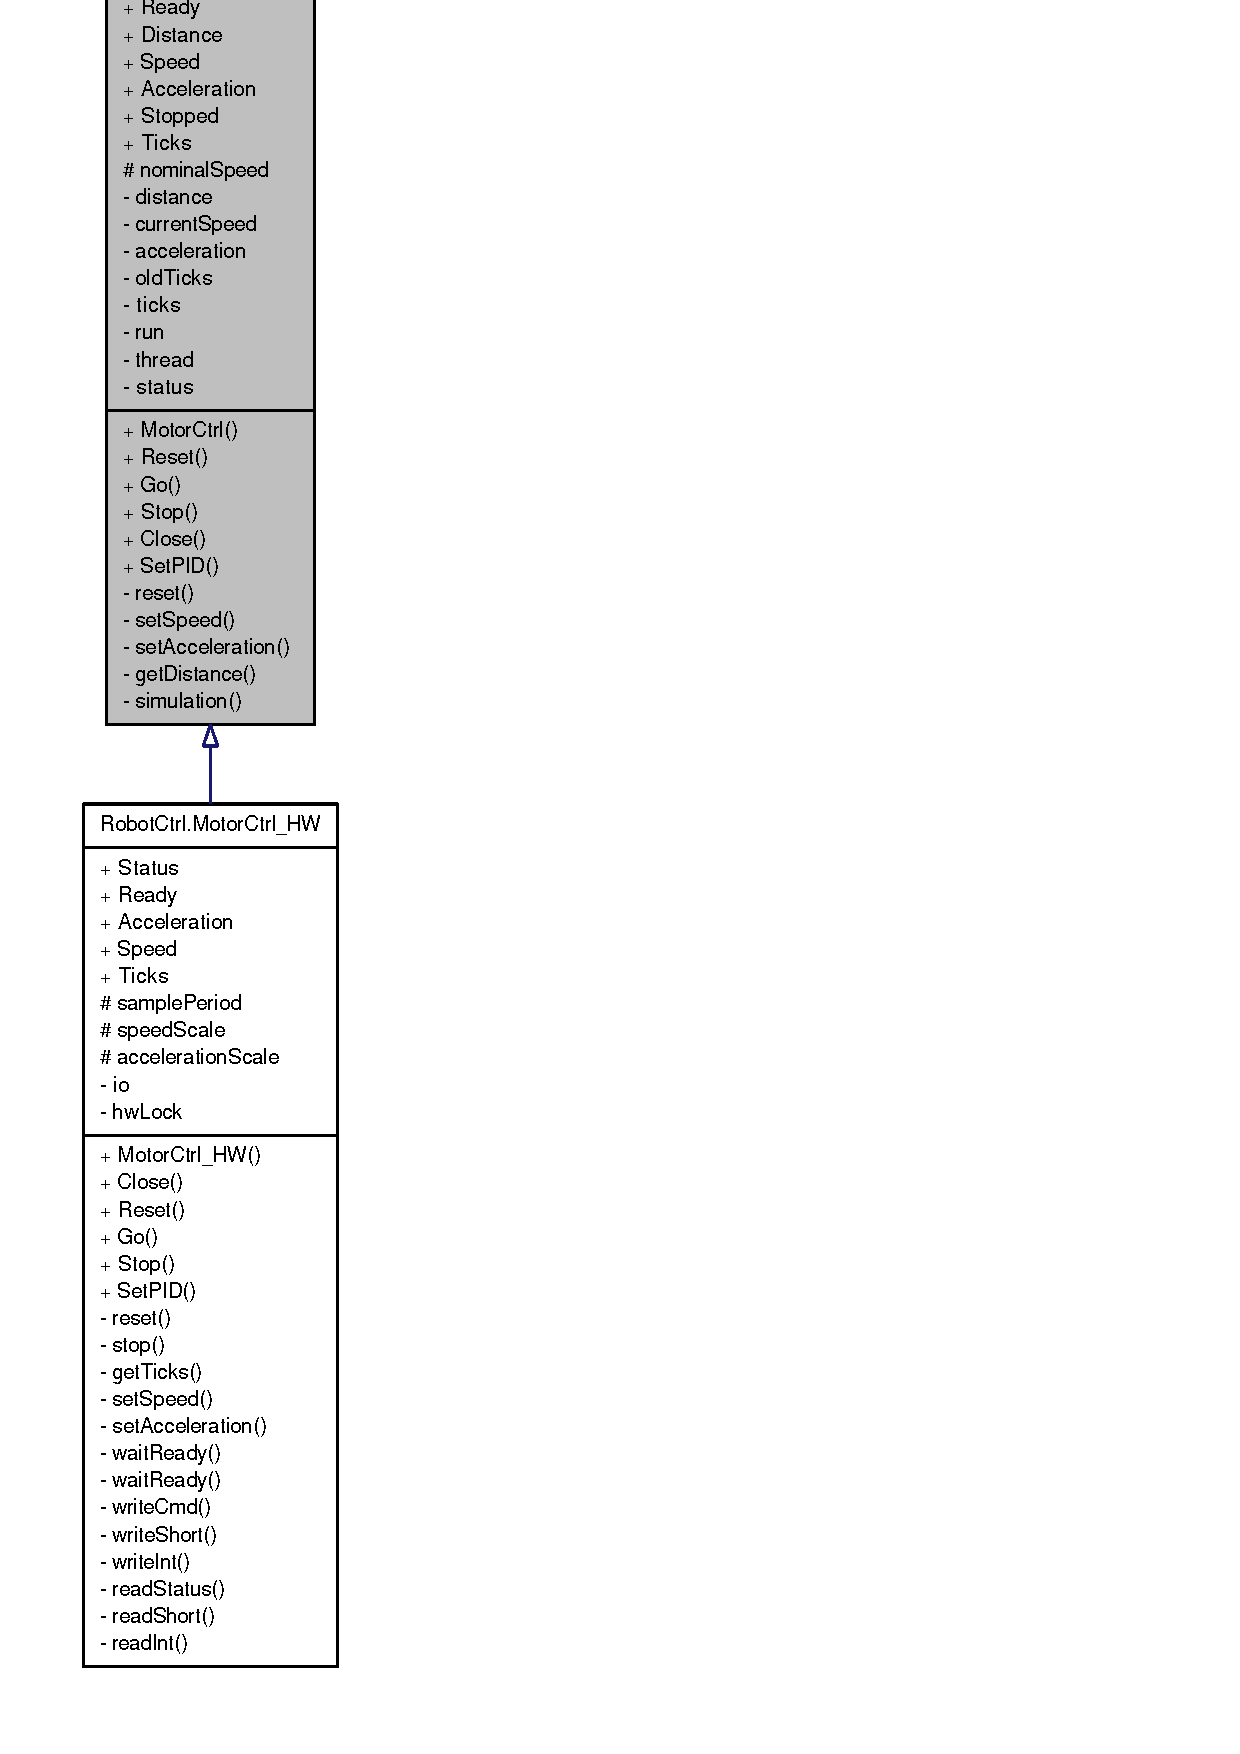
\includegraphics[height=400pt]{class_robot_ctrl_1_1_motor_ctrl__inherit__graph}
\end{center}
\end{figure}
\subsection*{Öffentliche Methoden}
\begin{DoxyCompactItemize}
\item 
\hypertarget{class_robot_ctrl_1_1_motor_ctrl_a57b1bb7cb3895bc5d867848926b57f1e}{
virtual void {\bfseries Reset} ()}
\label{class_robot_ctrl_1_1_motor_ctrl_a57b1bb7cb3895bc5d867848926b57f1e}

\item 
\hypertarget{class_robot_ctrl_1_1_motor_ctrl_a1c2505454168fc2d4287fe7052425d4e}{
virtual void {\bfseries Go} ()}
\label{class_robot_ctrl_1_1_motor_ctrl_a1c2505454168fc2d4287fe7052425d4e}

\item 
\hypertarget{class_robot_ctrl_1_1_motor_ctrl_a4e61bcac558a43dd2d1470ded5fed820}{
virtual void {\bfseries Stop} ()}
\label{class_robot_ctrl_1_1_motor_ctrl_a4e61bcac558a43dd2d1470ded5fed820}

\item 
\hypertarget{class_robot_ctrl_1_1_motor_ctrl_aa4d43c3586f611f8ca12924b0a92189b}{
virtual void {\bfseries Close} ()}
\label{class_robot_ctrl_1_1_motor_ctrl_aa4d43c3586f611f8ca12924b0a92189b}

\item 
\hypertarget{class_robot_ctrl_1_1_motor_ctrl_ac6e7ec6b155d337dddf2fe1bc660c11b}{
virtual void {\bfseries SetPID} (int proportional, int integral, int derivative, int integralLimit, int derivativeInterval)}
\label{class_robot_ctrl_1_1_motor_ctrl_ac6e7ec6b155d337dddf2fe1bc660c11b}

\end{DoxyCompactItemize}
\subsection*{Geschützte Attribute}
\begin{DoxyCompactItemize}
\item 
\hypertarget{class_robot_ctrl_1_1_motor_ctrl_a62360699e5fbae4b92c21e4b8cc9c823}{
double {\bfseries nominalSpeed}}
\label{class_robot_ctrl_1_1_motor_ctrl_a62360699e5fbae4b92c21e4b8cc9c823}

\end{DoxyCompactItemize}
\subsection*{Propertys}
\begin{DoxyCompactItemize}
\item 
\hypertarget{class_robot_ctrl_1_1_motor_ctrl_ac0f2ebafce89738ca669eaa920a30c80}{
virtual int {\bfseries Status}\hspace{0.3cm}{\ttfamily  \mbox{[}get\mbox{]}}}
\label{class_robot_ctrl_1_1_motor_ctrl_ac0f2ebafce89738ca669eaa920a30c80}

\item 
\hypertarget{class_robot_ctrl_1_1_motor_ctrl_a1152904081a4c96fa0bf27a6a48e728d}{
virtual bool {\bfseries Ready}\hspace{0.3cm}{\ttfamily  \mbox{[}get\mbox{]}}}
\label{class_robot_ctrl_1_1_motor_ctrl_a1152904081a4c96fa0bf27a6a48e728d}

\item 
\hypertarget{class_robot_ctrl_1_1_motor_ctrl_a7f1b09f359e4e09c85c9438a5de7dd9b}{
virtual double {\bfseries Distance}\hspace{0.3cm}{\ttfamily  \mbox{[}get, set\mbox{]}}}
\label{class_robot_ctrl_1_1_motor_ctrl_a7f1b09f359e4e09c85c9438a5de7dd9b}

\item 
\hypertarget{class_robot_ctrl_1_1_motor_ctrl_a13a5a1ee7896d0557c58ba617af60029}{
virtual double {\bfseries Speed}\hspace{0.3cm}{\ttfamily  \mbox{[}get, set\mbox{]}}}
\label{class_robot_ctrl_1_1_motor_ctrl_a13a5a1ee7896d0557c58ba617af60029}

\item 
\hypertarget{class_robot_ctrl_1_1_motor_ctrl_a57bbec274a01f59d5e5ede7599e0ca9f}{
virtual double {\bfseries Acceleration}\hspace{0.3cm}{\ttfamily  \mbox{[}set\mbox{]}}}
\label{class_robot_ctrl_1_1_motor_ctrl_a57bbec274a01f59d5e5ede7599e0ca9f}

\item 
\hypertarget{class_robot_ctrl_1_1_motor_ctrl_a5d2599ad295ece36d107cc7cb117d9c9}{
bool {\bfseries Stopped}\hspace{0.3cm}{\ttfamily  \mbox{[}get\mbox{]}}}
\label{class_robot_ctrl_1_1_motor_ctrl_a5d2599ad295ece36d107cc7cb117d9c9}

\item 
\hypertarget{class_robot_ctrl_1_1_motor_ctrl_a625a8335b71115e58d2d04c59027fb81}{
virtual int {\bfseries Ticks}\hspace{0.3cm}{\ttfamily  \mbox{[}get\mbox{]}}}
\label{class_robot_ctrl_1_1_motor_ctrl_a625a8335b71115e58d2d04c59027fb81}

\end{DoxyCompactItemize}


Die Dokumentation für diese Klasse wurde erzeugt aufgrund der Datei:\begin{DoxyCompactItemize}
\item 
MotorCtrl.cs\end{DoxyCompactItemize}

\hypertarget{class_robot_ctrl_1_1_motor_ctrl___h_w}{
\section{RobotCtrl.MotorCtrl\_\-HW Klassenreferenz}
\label{class_robot_ctrl_1_1_motor_ctrl___h_w}\index{RobotCtrl::MotorCtrl\_\-HW@{RobotCtrl::MotorCtrl\_\-HW}}
}


Klassendiagramm für RobotCtrl.MotorCtrl\_\-HW:\nopagebreak
\begin{figure}[H]
\begin{center}
\leavevmode
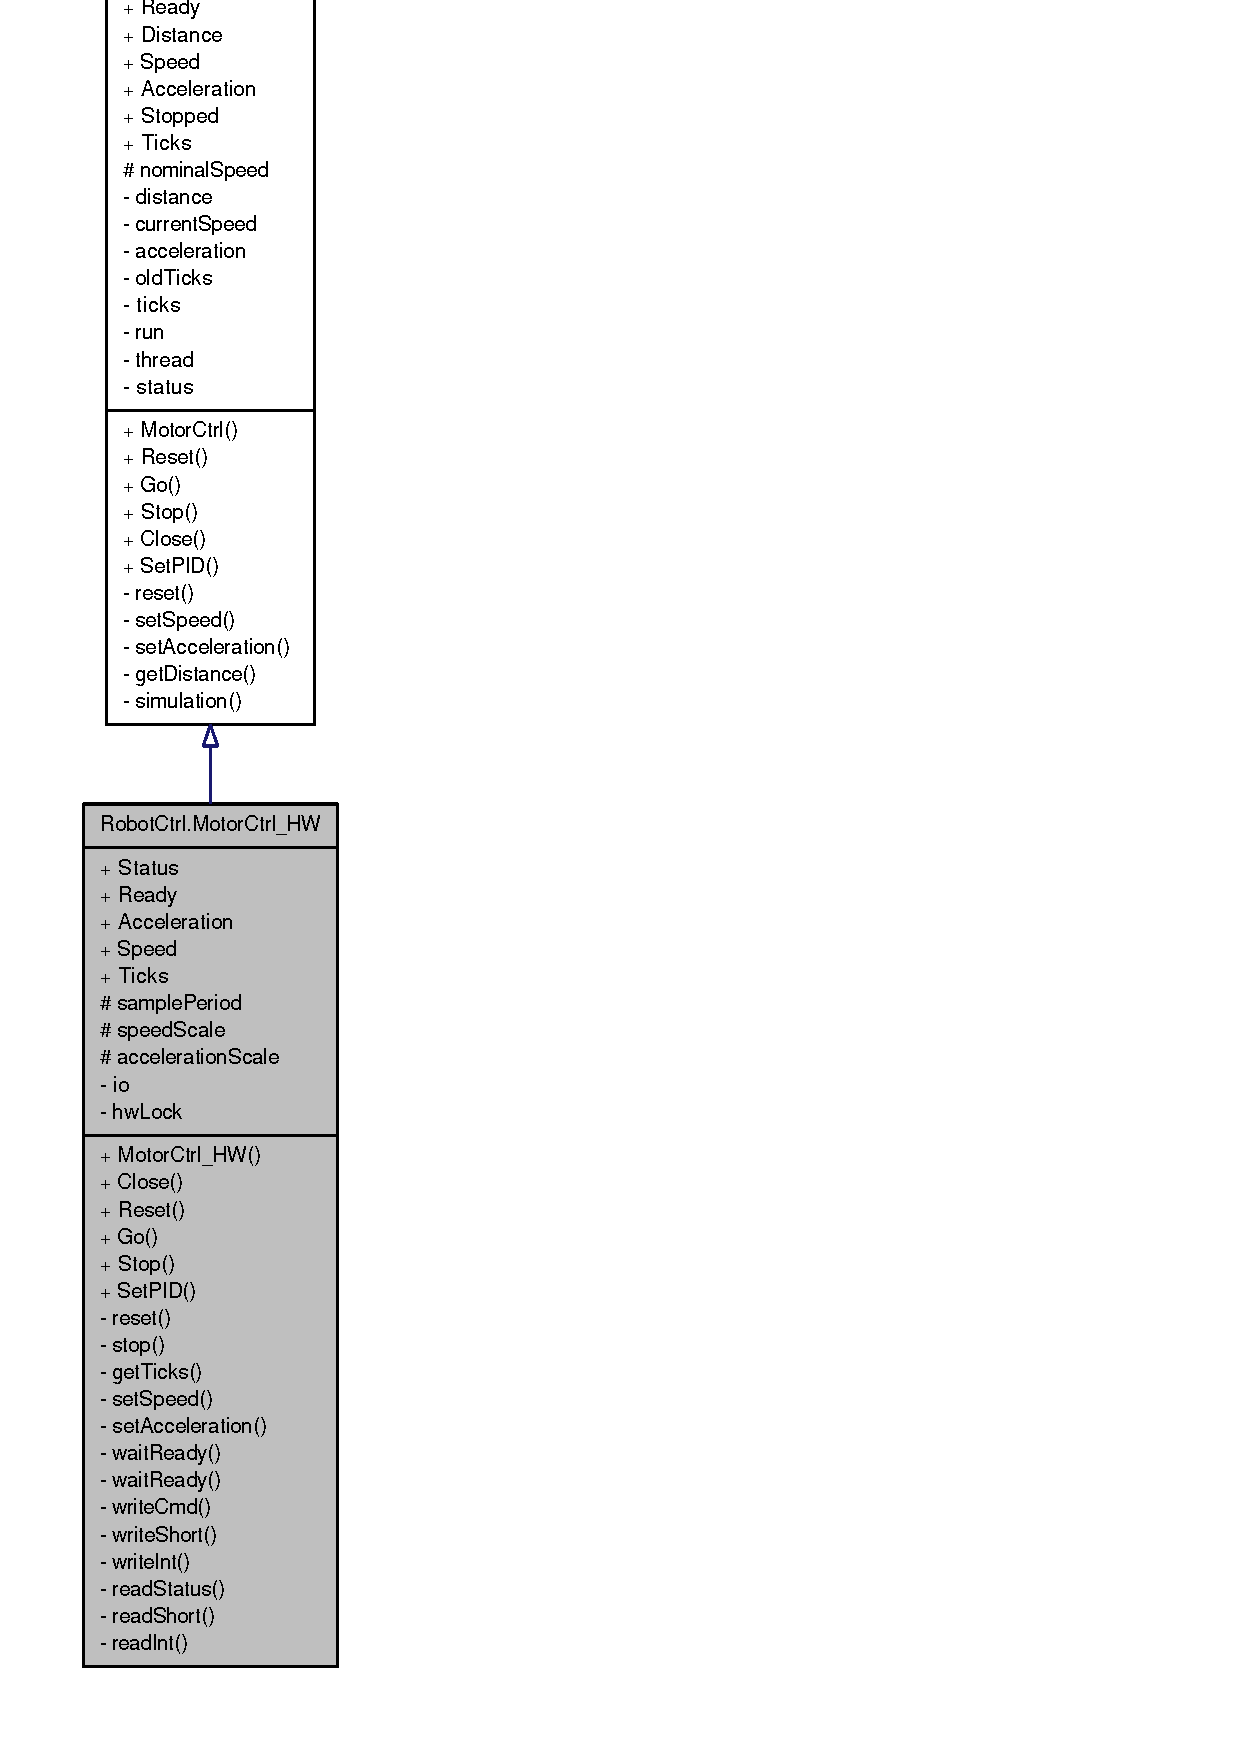
\includegraphics[height=400pt]{class_robot_ctrl_1_1_motor_ctrl___h_w__inherit__graph}
\end{center}
\end{figure}


Zusammengehörigkeiten von RobotCtrl.MotorCtrl\_\-HW:\nopagebreak
\begin{figure}[H]
\begin{center}
\leavevmode
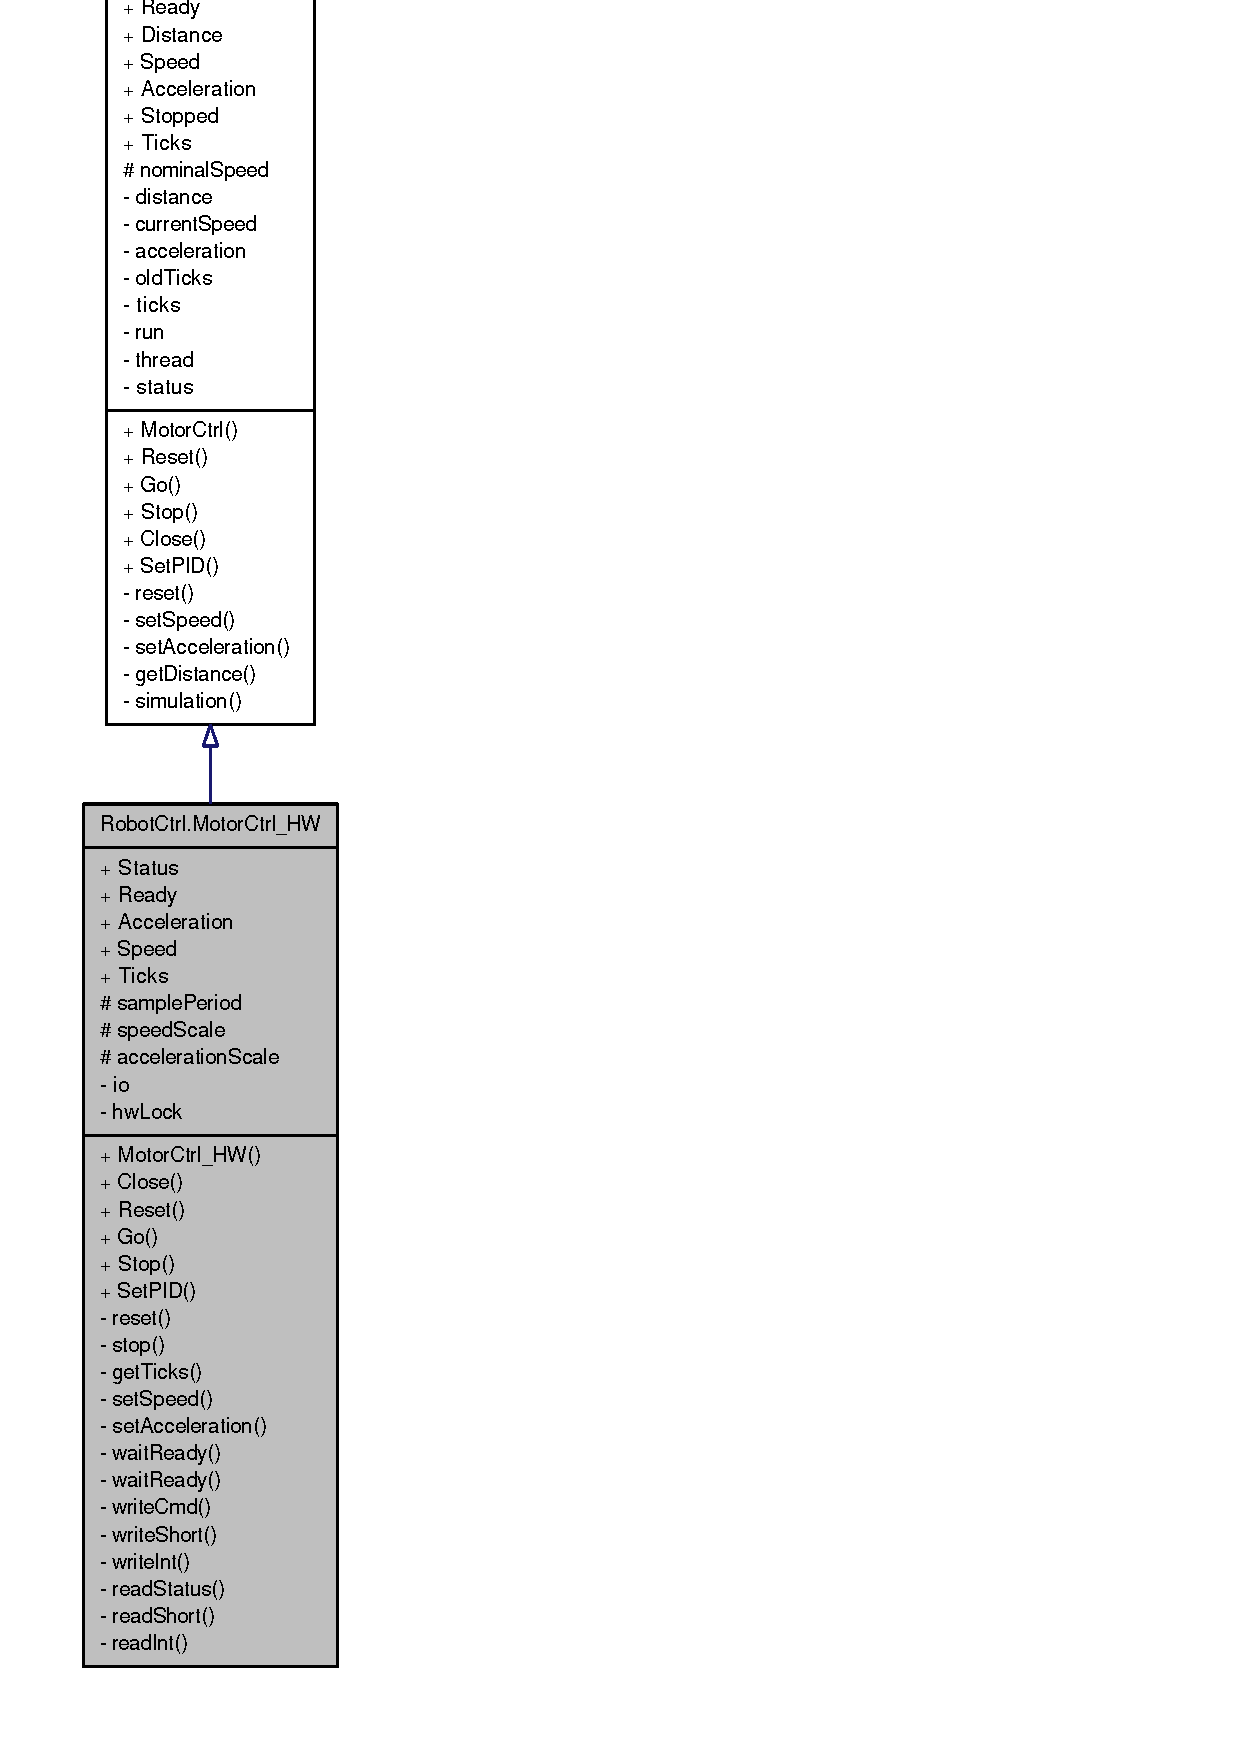
\includegraphics[height=400pt]{class_robot_ctrl_1_1_motor_ctrl___h_w__coll__graph}
\end{center}
\end{figure}
\subsection*{Öffentliche Methoden}
\begin{DoxyCompactItemize}
\item 
\hypertarget{class_robot_ctrl_1_1_motor_ctrl___h_w_af9fb7c75d12f00d852304d58bd31bcea}{
{\bfseries MotorCtrl\_\-HW} (int IOAddress)}
\label{class_robot_ctrl_1_1_motor_ctrl___h_w_af9fb7c75d12f00d852304d58bd31bcea}

\item 
\hypertarget{class_robot_ctrl_1_1_motor_ctrl___h_w_a134912d08a58d3762ce7694294599d7c}{
override void {\bfseries Close} ()}
\label{class_robot_ctrl_1_1_motor_ctrl___h_w_a134912d08a58d3762ce7694294599d7c}

\item 
\hypertarget{class_robot_ctrl_1_1_motor_ctrl___h_w_a1a116e83d87c50119567ff4ae334b239}{
override void {\bfseries Reset} ()}
\label{class_robot_ctrl_1_1_motor_ctrl___h_w_a1a116e83d87c50119567ff4ae334b239}

\item 
\hypertarget{class_robot_ctrl_1_1_motor_ctrl___h_w_a451b6be6938c652e8a284545a1929089}{
override void {\bfseries Go} ()}
\label{class_robot_ctrl_1_1_motor_ctrl___h_w_a451b6be6938c652e8a284545a1929089}

\item 
\hypertarget{class_robot_ctrl_1_1_motor_ctrl___h_w_ad7a992614ff75966b4381f8f8ef56cfd}{
override void {\bfseries Stop} ()}
\label{class_robot_ctrl_1_1_motor_ctrl___h_w_ad7a992614ff75966b4381f8f8ef56cfd}

\item 
\hypertarget{class_robot_ctrl_1_1_motor_ctrl___h_w_a24f22cd266cce1e701f9823e02816ff5}{
override void {\bfseries SetPID} (int proportional, int integral, int derivative, int integralLimit, int derivativeInterval)}
\label{class_robot_ctrl_1_1_motor_ctrl___h_w_a24f22cd266cce1e701f9823e02816ff5}

\end{DoxyCompactItemize}
\subsection*{Geschützte Attribute}
\begin{DoxyCompactItemize}
\item 
\hypertarget{class_robot_ctrl_1_1_motor_ctrl___h_w_a9b2e8f281c704b73014ed11f838dfab5}{
const double {\bfseries samplePeriod} = 256E-\/6}
\label{class_robot_ctrl_1_1_motor_ctrl___h_w_a9b2e8f281c704b73014ed11f838dfab5}

\item 
\hypertarget{class_robot_ctrl_1_1_motor_ctrl___h_w_a054d80af56e02234681d2ad157be9376}{
const double {\bfseries speedScale} = samplePeriod / Config.MeterPerTick $\ast$ (1 $<$$<$ 16)}
\label{class_robot_ctrl_1_1_motor_ctrl___h_w_a054d80af56e02234681d2ad157be9376}

\item 
\hypertarget{class_robot_ctrl_1_1_motor_ctrl___h_w_aae79f545c62e3a7dbbd0efd6d434c68e}{
const double {\bfseries accelerationScale} = samplePeriod $\ast$ samplePeriod / Config.MeterPerTick $\ast$ (1 $<$$<$ 16)}
\label{class_robot_ctrl_1_1_motor_ctrl___h_w_aae79f545c62e3a7dbbd0efd6d434c68e}

\end{DoxyCompactItemize}
\subsection*{Propertys}
\begin{DoxyCompactItemize}
\item 
\hypertarget{class_robot_ctrl_1_1_motor_ctrl___h_w_a0c39f88363e68b382cf946f37fe98e16}{
override int {\bfseries Status}\hspace{0.3cm}{\ttfamily  \mbox{[}get\mbox{]}}}
\label{class_robot_ctrl_1_1_motor_ctrl___h_w_a0c39f88363e68b382cf946f37fe98e16}

\item 
\hypertarget{class_robot_ctrl_1_1_motor_ctrl___h_w_aa5f0c2dd90cf577ef951e58e957976c9}{
override bool {\bfseries Ready}\hspace{0.3cm}{\ttfamily  \mbox{[}get\mbox{]}}}
\label{class_robot_ctrl_1_1_motor_ctrl___h_w_aa5f0c2dd90cf577ef951e58e957976c9}

\item 
\hypertarget{class_robot_ctrl_1_1_motor_ctrl___h_w_aeee6ccb14bb1c24c2541c64c0ad91c0e}{
override double {\bfseries Acceleration}\hspace{0.3cm}{\ttfamily  \mbox{[}set\mbox{]}}}
\label{class_robot_ctrl_1_1_motor_ctrl___h_w_aeee6ccb14bb1c24c2541c64c0ad91c0e}

\item 
\hypertarget{class_robot_ctrl_1_1_motor_ctrl___h_w_a037b7d7d65571c8eda634bef767a1870}{
override double {\bfseries Speed}\hspace{0.3cm}{\ttfamily  \mbox{[}get, set\mbox{]}}}
\label{class_robot_ctrl_1_1_motor_ctrl___h_w_a037b7d7d65571c8eda634bef767a1870}

\item 
\hypertarget{class_robot_ctrl_1_1_motor_ctrl___h_w_a22603ba1614f7f9eb88f2b7ea0a4c700}{
override int {\bfseries Ticks}\hspace{0.3cm}{\ttfamily  \mbox{[}get\mbox{]}}}
\label{class_robot_ctrl_1_1_motor_ctrl___h_w_a22603ba1614f7f9eb88f2b7ea0a4c700}

\end{DoxyCompactItemize}


Die Dokumentation für diese Klasse wurde erzeugt aufgrund der Datei:\begin{DoxyCompactItemize}
\item 
MotorCtrl\_\-HW.cs\end{DoxyCompactItemize}

\hypertarget{class_robot_ctrl_1_1_obstacle_map}{
\section{RobotCtrl.ObstacleMap Klassenreferenz}
\label{class_robot_ctrl_1_1_obstacle_map}\index{RobotCtrl::ObstacleMap@{RobotCtrl::ObstacleMap}}
}
\subsection*{Öffentliche Methoden}
\begin{DoxyCompactItemize}
\item 
\hypertarget{class_robot_ctrl_1_1_obstacle_map_aa685bbf8cef8ae30c8a2a59a602f44b9}{
{\bfseries ObstacleMap} (RectangleF area, Bitmap map)}
\label{class_robot_ctrl_1_1_obstacle_map_aa685bbf8cef8ae30c8a2a59a602f44b9}

\item 
\hypertarget{class_robot_ctrl_1_1_obstacle_map_a6331e9073a17ee26ba3e272f4f20122f}{
Bitmap {\bfseries getImage} ()}
\label{class_robot_ctrl_1_1_obstacle_map_a6331e9073a17ee26ba3e272f4f20122f}

\end{DoxyCompactItemize}
\subsection*{Propertys}
\begin{DoxyCompactItemize}
\item 
\hypertarget{class_robot_ctrl_1_1_obstacle_map_a62cd370edbb98ccfd63af84f52c92e34}{
RectangleF {\bfseries dimension}\hspace{0.3cm}{\ttfamily  \mbox{[}get, set\mbox{]}}}
\label{class_robot_ctrl_1_1_obstacle_map_a62cd370edbb98ccfd63af84f52c92e34}

\end{DoxyCompactItemize}


Die Dokumentation für diese Klasse wurde erzeugt aufgrund der Datei:\begin{DoxyCompactItemize}
\item 
ObstacleMap.cs\end{DoxyCompactItemize}

\hypertarget{struct_robot_ctrl_1_1_position_info}{
\section{RobotCtrl.PositionInfo Strukturreferenz}
\label{struct_robot_ctrl_1_1_position_info}\index{RobotCtrl::PositionInfo@{RobotCtrl::PositionInfo}}
}
\subsection*{Öffentliche Methoden}
\begin{DoxyCompactItemize}
\item 
\hypertarget{struct_robot_ctrl_1_1_position_info_a437f826ea5eb342dc35bdf9100c38b69}{
{\bfseries PositionInfo} (double x, double y, double angle)}
\label{struct_robot_ctrl_1_1_position_info_a437f826ea5eb342dc35bdf9100c38b69}

\end{DoxyCompactItemize}
\subsection*{Öffentliche Attribute}
\begin{DoxyCompactItemize}
\item 
\hypertarget{struct_robot_ctrl_1_1_position_info_a004e97e7977e8a19966104d0d1f3de84}{
double {\bfseries X}}
\label{struct_robot_ctrl_1_1_position_info_a004e97e7977e8a19966104d0d1f3de84}

\item 
\hypertarget{struct_robot_ctrl_1_1_position_info_a4e06789a38efca8072df7b9f21cd552e}{
double {\bfseries Y}}
\label{struct_robot_ctrl_1_1_position_info_a4e06789a38efca8072df7b9f21cd552e}

\item 
\hypertarget{struct_robot_ctrl_1_1_position_info_a12ed93794ca7fc28db9b5ce3afb53da3}{
double {\bfseries Angle}}
\label{struct_robot_ctrl_1_1_position_info_a12ed93794ca7fc28db9b5ce3afb53da3}

\end{DoxyCompactItemize}


Die Dokumentation für diese Struktur wurde erzeugt aufgrund der Datei:\begin{DoxyCompactItemize}
\item 
PositionInfo.cs\end{DoxyCompactItemize}

\hypertarget{class_robot_ctrl_1_1_radar}{
\section{RobotCtrl.Radar Klassenreferenz}
\label{class_robot_ctrl_1_1_radar}\index{RobotCtrl::Radar@{RobotCtrl::Radar}}
}


Klasse \hyperlink{class_robot_ctrl_1_1_radar}{Radar} dient der Orientierung des \hyperlink{class_robot_ctrl_1_1_robot}{Robot}.  




Zusammengehörigkeiten von RobotCtrl.Radar:\subsection*{Öffentliche Methoden}
\begin{DoxyCompactItemize}
\item 
\hyperlink{class_robot_ctrl_1_1_radar_aec75e7f4e126ac40c008c5d30d1c8dba}{Radar} (\hyperlink{class_robot_ctrl_1_1_robot}{Robot} robot, RunMode runMode)
\end{DoxyCompactItemize}
\subsection*{Propertys}
\begin{DoxyCompactItemize}
\item 
double \hyperlink{class_robot_ctrl_1_1_radar_a0339d462806cb7fc3759d850b5564dd9}{Distance}\hspace{0.3cm}{\ttfamily  \mbox{[}get\mbox{]}}
\end{DoxyCompactItemize}


\subsection{Ausführliche Beschreibung}
Klasse \hyperlink{class_robot_ctrl_1_1_radar}{Radar} dient der Orientierung des \hyperlink{class_robot_ctrl_1_1_robot}{Robot}. 

\subsection{Beschreibung der Konstruktoren und Destruktoren}
\hypertarget{class_robot_ctrl_1_1_radar_aec75e7f4e126ac40c008c5d30d1c8dba}{
\index{RobotCtrl::Radar@{RobotCtrl::Radar}!Radar@{Radar}}
\index{Radar@{Radar}!RobotCtrl::Radar@{RobotCtrl::Radar}}
\subsubsection[{Radar}]{\setlength{\rightskip}{0pt plus 5cm}RobotCtrl.Radar.Radar ({\bf Robot} {\em robot}, \/  RunMode {\em runMode})}}
\label{class_robot_ctrl_1_1_radar_aec75e7f4e126ac40c008c5d30d1c8dba}
Konstruktor f\"{u}r einen \hyperlink{class_robot_ctrl_1_1_radar}{Radar} \begin{DoxySeeAlso}{Siehe auch}
\hyperlink{class_robot_ctrl_1_1_config}{Config}
\end{DoxySeeAlso}

\begin{DoxyParams}{Parameter}
\item[{\em robot}]Referenz auf einen \hyperlink{class_robot_ctrl_1_1_robot}{Robot} \item[{\em runMode}]Der Runmode \end{DoxyParams}


\subsection{Dokumentation der Propertys}
\hypertarget{class_robot_ctrl_1_1_radar_a0339d462806cb7fc3759d850b5564dd9}{
\index{RobotCtrl::Radar@{RobotCtrl::Radar}!Distance@{Distance}}
\index{Distance@{Distance}!RobotCtrl::Radar@{RobotCtrl::Radar}}
\subsubsection[{Distance}]{\setlength{\rightskip}{0pt plus 5cm}double RobotCtrl.Radar.Distance\hspace{0.3cm}{\ttfamily  \mbox{[}get\mbox{]}}}}
\label{class_robot_ctrl_1_1_radar_a0339d462806cb7fc3759d850b5564dd9}
Property Distance gibt die Distanz zu einem Hindernis zur\"{u}ck. 

Die Dokumentation für diese Klasse wurde erzeugt aufgrund der Datei:\begin{DoxyCompactItemize}
\item 
Radar.cs\end{DoxyCompactItemize}

\hypertarget{class_robot_ctrl_1_1_radar_sensor}{
\section{RobotCtrl.RadarSensor Klassenreferenz}
\label{class_robot_ctrl_1_1_radar_sensor}\index{RobotCtrl::RadarSensor@{RobotCtrl::RadarSensor}}
}


\hyperlink{class_robot_ctrl_1_1_radar_sensor}{RadarSensor} ist ein Sensor.  




Klassendiagramm für RobotCtrl.RadarSensor:\nopagebreak
\begin{figure}[H]
\begin{center}
\leavevmode
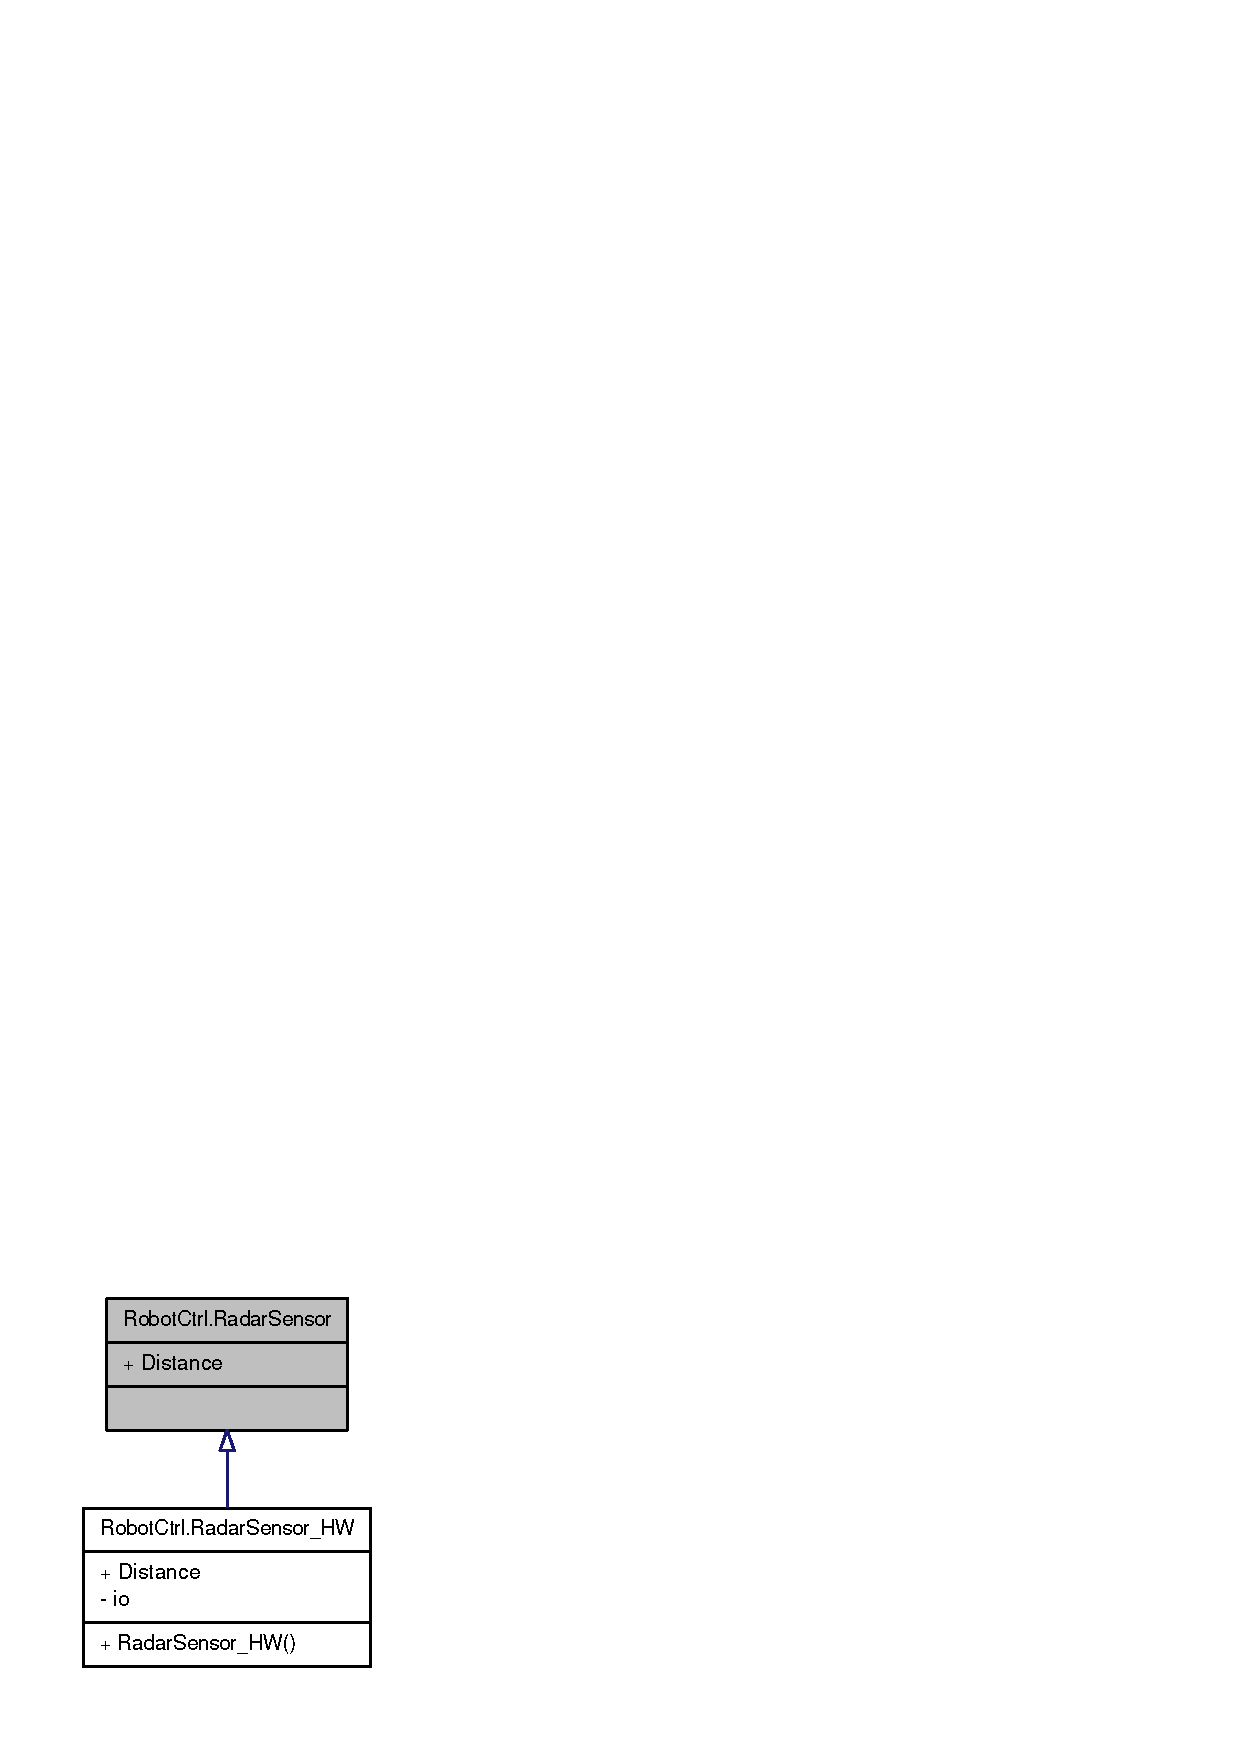
\includegraphics[width=182pt]{class_robot_ctrl_1_1_radar_sensor__inherit__graph}
\end{center}
\end{figure}
\subsection*{Propertys}
\begin{DoxyCompactItemize}
\item 
virtual double \hyperlink{class_robot_ctrl_1_1_radar_sensor_a1be5541f3153ba40736f7a9fa292375b}{Distance}\hspace{0.3cm}{\ttfamily  \mbox{[}get\mbox{]}}
\end{DoxyCompactItemize}


\subsection{Ausführliche Beschreibung}
\hyperlink{class_robot_ctrl_1_1_radar_sensor}{RadarSensor} ist ein Sensor. 

\subsection{Dokumentation der Propertys}
\hypertarget{class_robot_ctrl_1_1_radar_sensor_a1be5541f3153ba40736f7a9fa292375b}{
\index{RobotCtrl::RadarSensor@{RobotCtrl::RadarSensor}!Distance@{Distance}}
\index{Distance@{Distance}!RobotCtrl::RadarSensor@{RobotCtrl::RadarSensor}}
\subsubsection[{Distance}]{\setlength{\rightskip}{0pt plus 5cm}virtual double RobotCtrl.RadarSensor.Distance\hspace{0.3cm}{\ttfamily  \mbox{[}get\mbox{]}}}}
\label{class_robot_ctrl_1_1_radar_sensor_a1be5541f3153ba40736f7a9fa292375b}
Property um die Distanz zu einem Hindernis in Erfahrung zu bringen 

Erneute Implementation in \hyperlink{class_robot_ctrl_1_1_radar_sensor___h_w_a0eb1060a6e45bb29fdbf99e35481311e}{RobotCtrl.RadarSensor\_\-HW}.



Die Dokumentation für diese Klasse wurde erzeugt aufgrund der Datei:\begin{DoxyCompactItemize}
\item 
RadarSensor.cs\end{DoxyCompactItemize}

\hypertarget{class_robot_ctrl_1_1_radar_sensor___h_w}{
\section{RobotCtrl.RadarSensor\_\-HW Klassenreferenz}
\label{class_robot_ctrl_1_1_radar_sensor___h_w}\index{RobotCtrl::RadarSensor\_\-HW@{RobotCtrl::RadarSensor\_\-HW}}
}


\hyperlink{class_robot_ctrl_1_1_radar_sensor___h_w}{RadarSensor\_\-HW} erbt von \hyperlink{class_robot_ctrl_1_1_radar_sensor}{RadarSensor} und interagiert mit der Hardware.  




Klassendiagramm für RobotCtrl.RadarSensor\_\-HW:\nopagebreak
\begin{figure}[H]
\begin{center}
\leavevmode
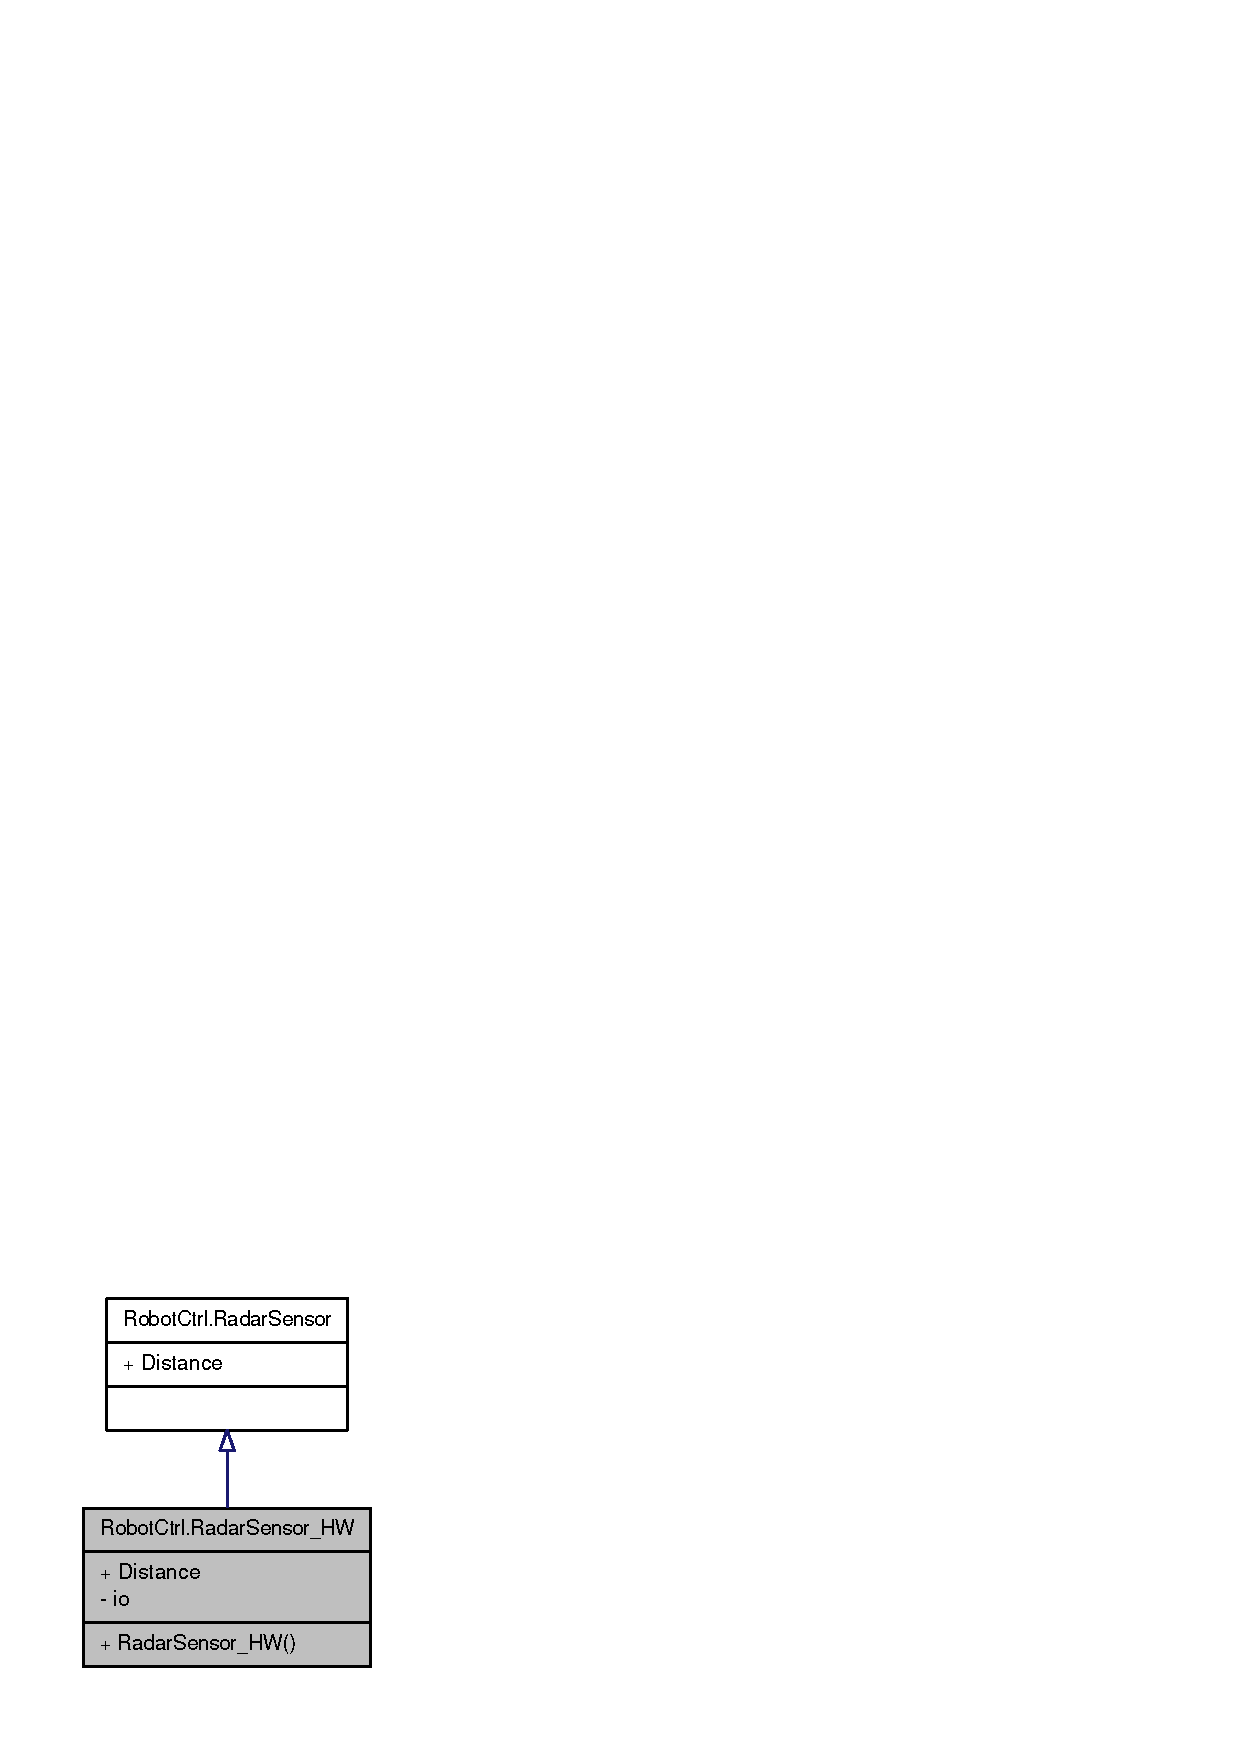
\includegraphics[width=182pt]{class_robot_ctrl_1_1_radar_sensor___h_w__inherit__graph}
\end{center}
\end{figure}


Zusammengehörigkeiten von RobotCtrl.RadarSensor\_\-HW:\nopagebreak
\begin{figure}[H]
\begin{center}
\leavevmode
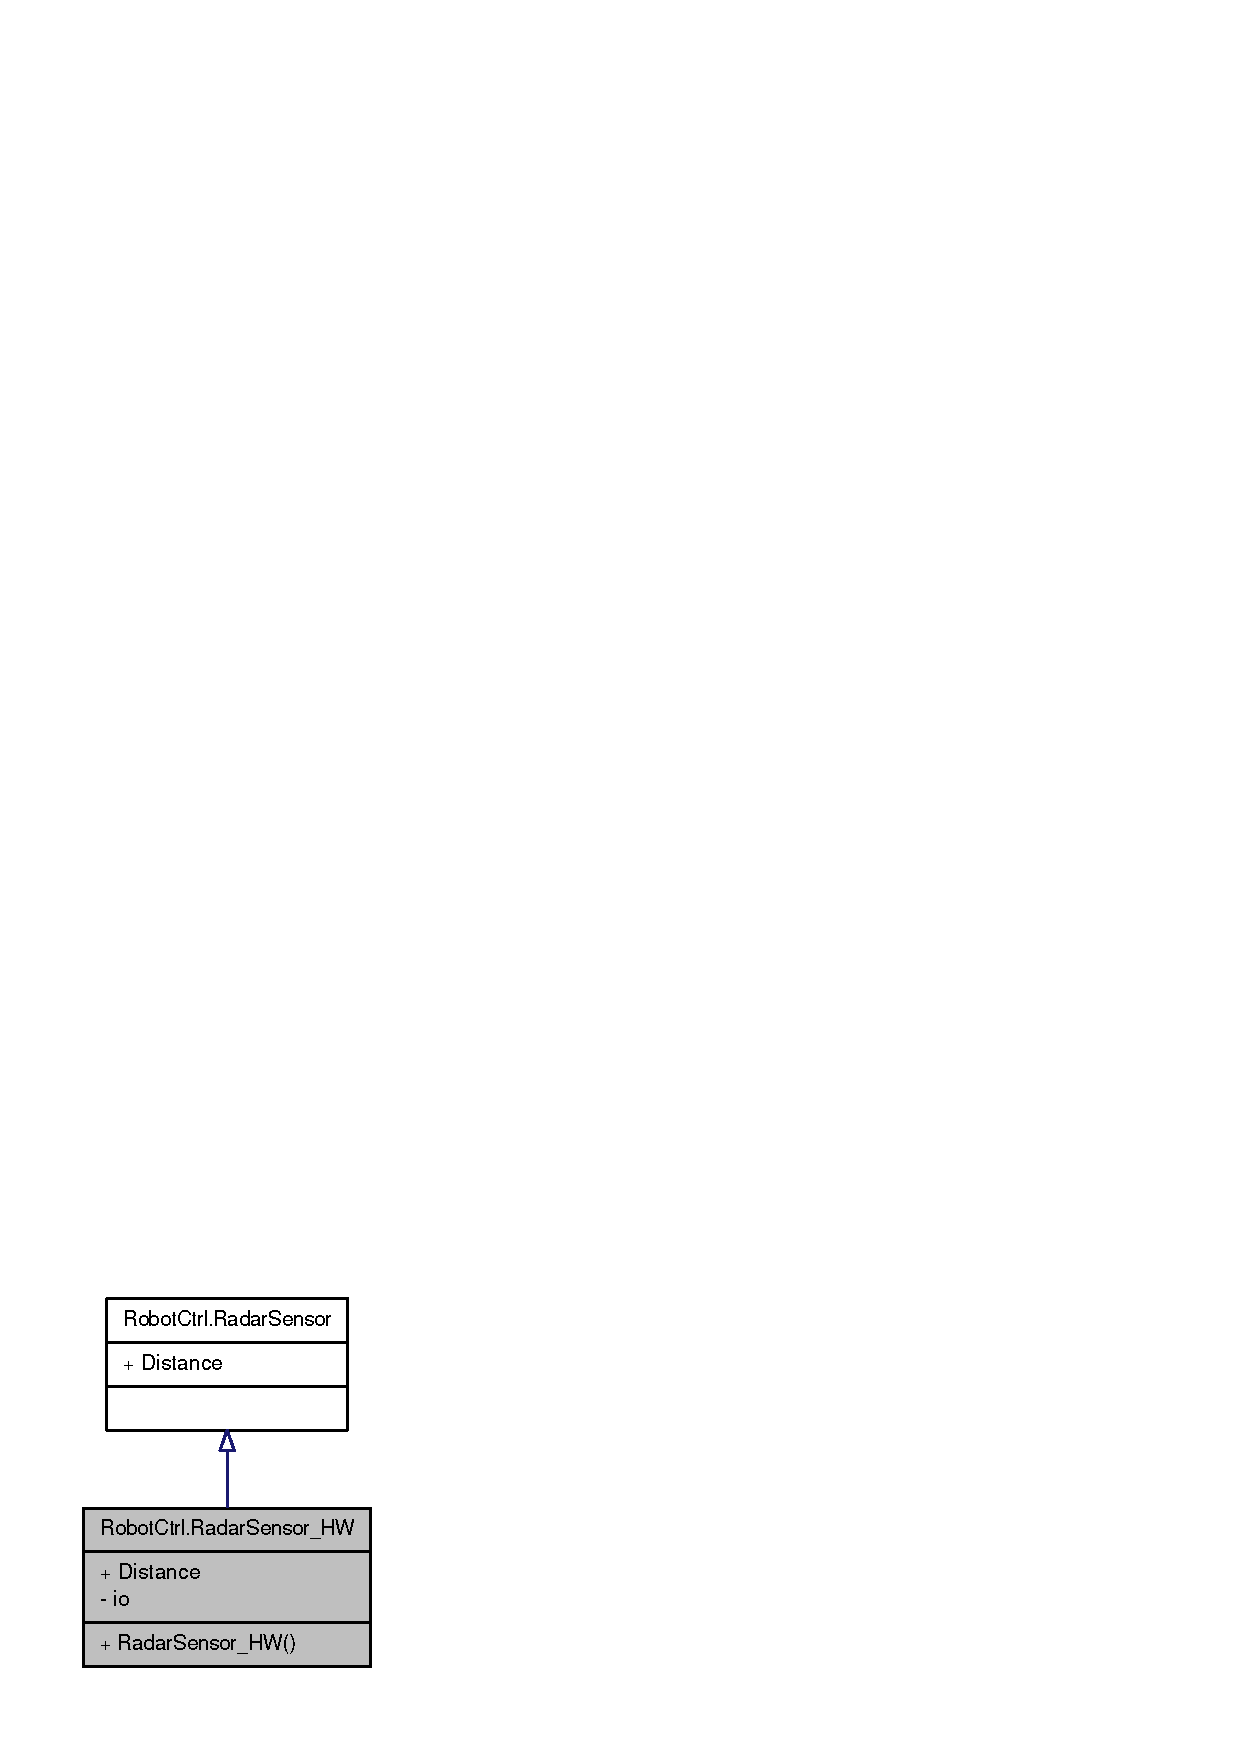
\includegraphics[width=182pt]{class_robot_ctrl_1_1_radar_sensor___h_w__coll__graph}
\end{center}
\end{figure}
\subsection*{Öffentliche Methoden}
\begin{DoxyCompactItemize}
\item 
\hyperlink{class_robot_ctrl_1_1_radar_sensor___h_w_a7730198b6097b06b30539165d3ca4953}{RadarSensor\_\-HW} (int IOAddress)
\end{DoxyCompactItemize}
\subsection*{Propertys}
\begin{DoxyCompactItemize}
\item 
override double \hyperlink{class_robot_ctrl_1_1_radar_sensor___h_w_a0eb1060a6e45bb29fdbf99e35481311e}{Distance}\hspace{0.3cm}{\ttfamily  \mbox{[}get\mbox{]}}
\end{DoxyCompactItemize}


\subsection{Ausführliche Beschreibung}
\hyperlink{class_robot_ctrl_1_1_radar_sensor___h_w}{RadarSensor\_\-HW} erbt von \hyperlink{class_robot_ctrl_1_1_radar_sensor}{RadarSensor} und interagiert mit der Hardware. 

\subsection{Beschreibung der Konstruktoren und Destruktoren}
\hypertarget{class_robot_ctrl_1_1_radar_sensor___h_w_a7730198b6097b06b30539165d3ca4953}{
\index{RobotCtrl::RadarSensor\_\-HW@{RobotCtrl::RadarSensor\_\-HW}!RadarSensor\_\-HW@{RadarSensor\_\-HW}}
\index{RadarSensor\_\-HW@{RadarSensor\_\-HW}!RobotCtrl::RadarSensor_HW@{RobotCtrl::RadarSensor\_\-HW}}
\subsubsection[{RadarSensor\_\-HW}]{\setlength{\rightskip}{0pt plus 5cm}RobotCtrl.RadarSensor\_\-HW.RadarSensor\_\-HW (int {\em IOAddress})}}
\label{class_robot_ctrl_1_1_radar_sensor___h_w_a7730198b6097b06b30539165d3ca4953}
Konstruktor \hyperlink{class_robot_ctrl_1_1_radar_sensor___h_w}{RadarSensor\_\-HW}


\begin{DoxyParams}{Parameter}
\item[{\em IOAddress}]Hardware Adresse des Sensors \end{DoxyParams}


\subsection{Dokumentation der Propertys}
\hypertarget{class_robot_ctrl_1_1_radar_sensor___h_w_a0eb1060a6e45bb29fdbf99e35481311e}{
\index{RobotCtrl::RadarSensor\_\-HW@{RobotCtrl::RadarSensor\_\-HW}!Distance@{Distance}}
\index{Distance@{Distance}!RobotCtrl::RadarSensor_HW@{RobotCtrl::RadarSensor\_\-HW}}
\subsubsection[{Distance}]{\setlength{\rightskip}{0pt plus 5cm}override double RobotCtrl.RadarSensor\_\-HW.Distance\hspace{0.3cm}{\ttfamily  \mbox{[}get\mbox{]}}}}
\label{class_robot_ctrl_1_1_radar_sensor___h_w_a0eb1060a6e45bb29fdbf99e35481311e}
Property Distance gibt die Distanz, welche vom Sensor gemessen wurde zur\"{u}ck. 

Erneute Implementation von \hyperlink{class_robot_ctrl_1_1_radar_sensor_a1be5541f3153ba40736f7a9fa292375b}{RobotCtrl.RadarSensor}.



Die Dokumentation für diese Klasse wurde erzeugt aufgrund der Datei:\begin{DoxyCompactItemize}
\item 
RadarSensor\_\-HW.cs\end{DoxyCompactItemize}

\hypertarget{class_robot_view_1_1_resource1}{
\section{RobotView.Resource1 Klassenreferenz}
\label{class_robot_view_1_1_resource1}\index{RobotView::Resource1@{RobotView::Resource1}}
}


Eine stark typisierte Ressourcenklasse zum Suchen von lokalisierten Zeichenfolgen usw.  




\subsection{Ausführliche Beschreibung}
Eine stark typisierte Ressourcenklasse zum Suchen von lokalisierten Zeichenfolgen usw. 

Die Dokumentation für diese Klasse wurde erzeugt aufgrund der Datei:\begin{DoxyCompactItemize}
\item 
Resource1.Designer.cs\end{DoxyCompactItemize}

\hypertarget{class_test___console_1_1_properties_1_1_resources}{
\section{Test\_\-Console.Properties.Resources Klassenreferenz}
\label{class_test___console_1_1_properties_1_1_resources}\index{Test\_\-Console::Properties::Resources@{Test\_\-Console::Properties::Resources}}
}


Eine stark typisierte Ressourcenklasse zum Suchen von lokalisierten Zeichenfolgen usw.  




Zusammengehörigkeiten von Test\_\-Console.Properties.Resources:\nopagebreak
\begin{figure}[H]
\begin{center}
\leavevmode
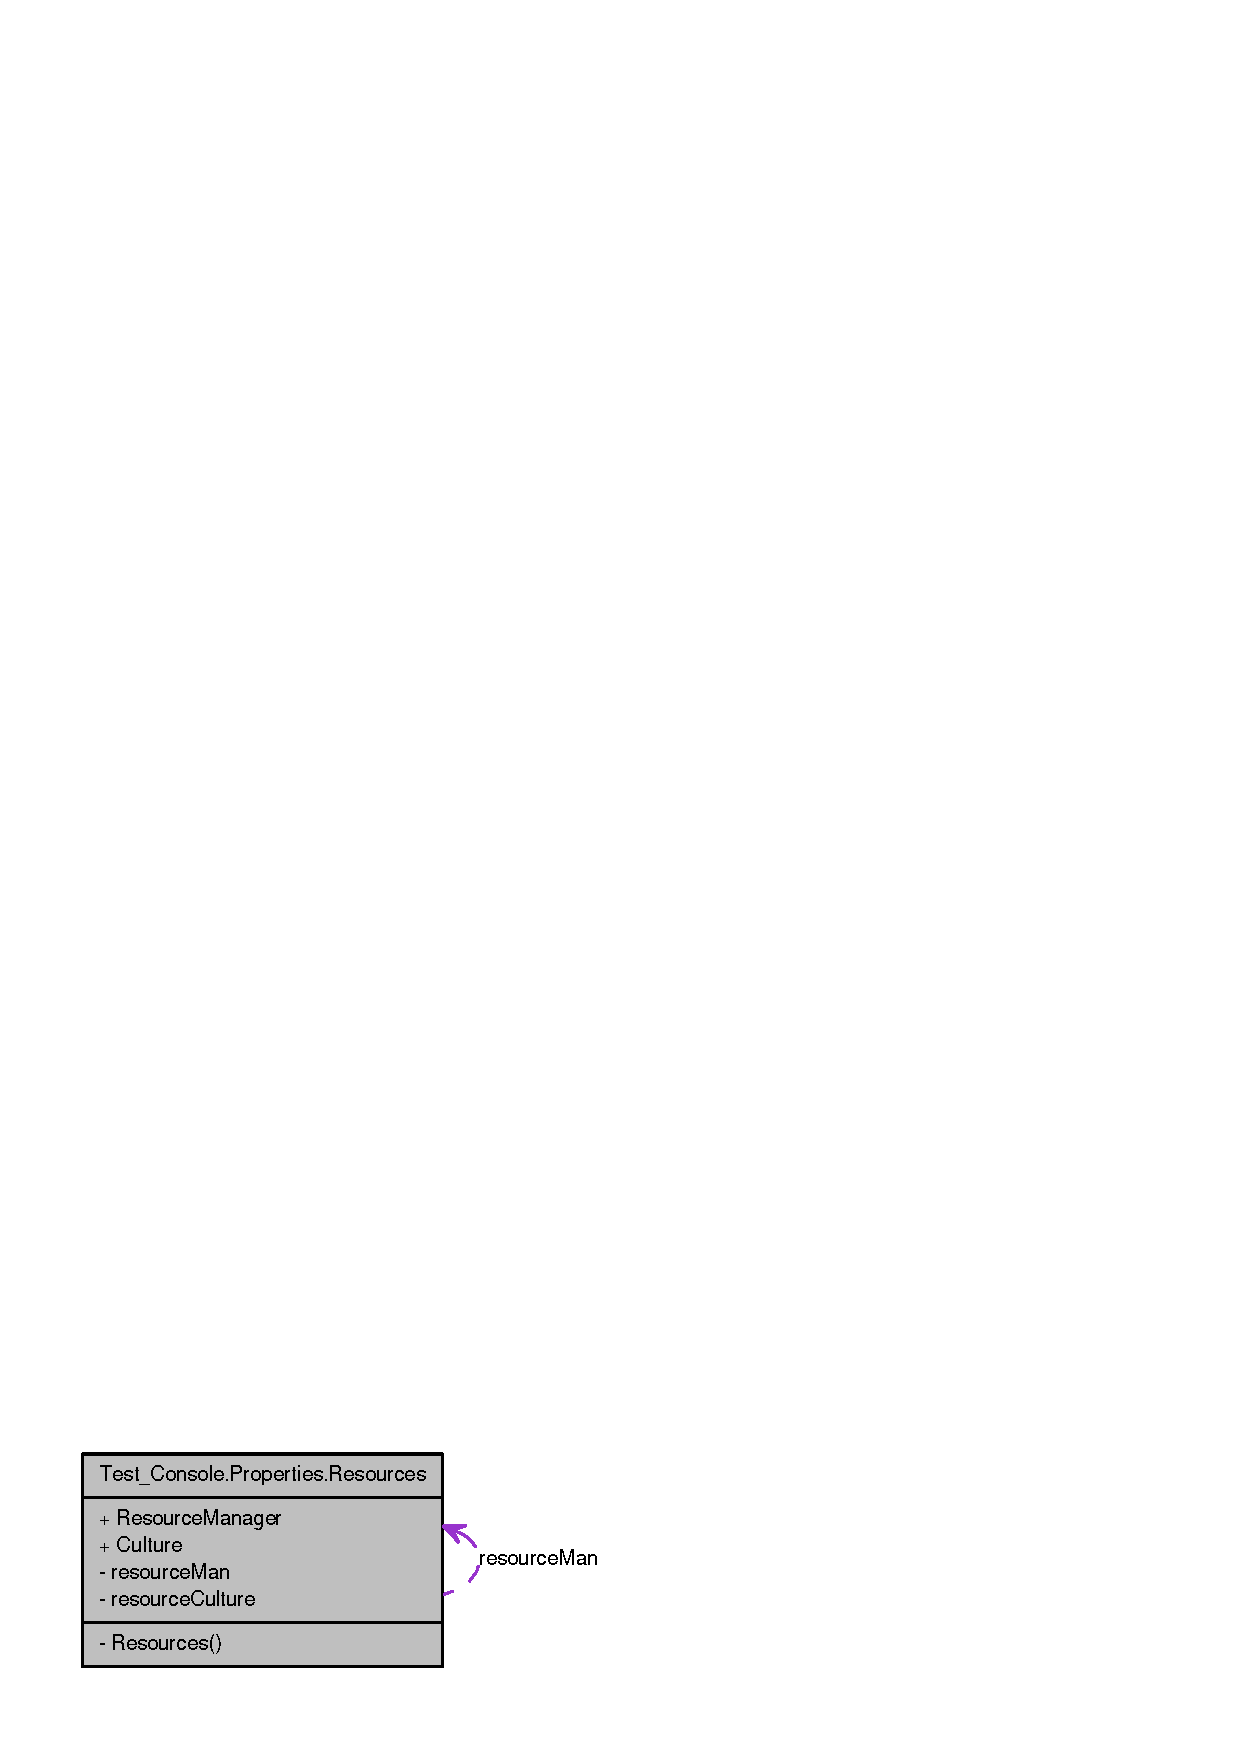
\includegraphics[width=291pt]{class_test___console_1_1_properties_1_1_resources__coll__graph}
\end{center}
\end{figure}


\subsection{Ausführliche Beschreibung}
Eine stark typisierte Ressourcenklasse zum Suchen von lokalisierten Zeichenfolgen usw. 

Die Dokumentation für diese Klasse wurde erzeugt aufgrund der Datei:\begin{DoxyCompactItemize}
\item 
Test-\/Console/Properties/Resources.Designer.cs\end{DoxyCompactItemize}

\hypertarget{class_test___world_1_1_properties_1_1_resources}{
\section{Test\_\-World.Properties.Resources Klassenreferenz}
\label{class_test___world_1_1_properties_1_1_resources}\index{Test\_\-World::Properties::Resources@{Test\_\-World::Properties::Resources}}
}


A strongly-\/typed resource class, for looking up localized strings, etc.  




Zusammengehörigkeiten von Test\_\-World.Properties.Resources:\nopagebreak
\begin{figure}[H]
\begin{center}
\leavevmode
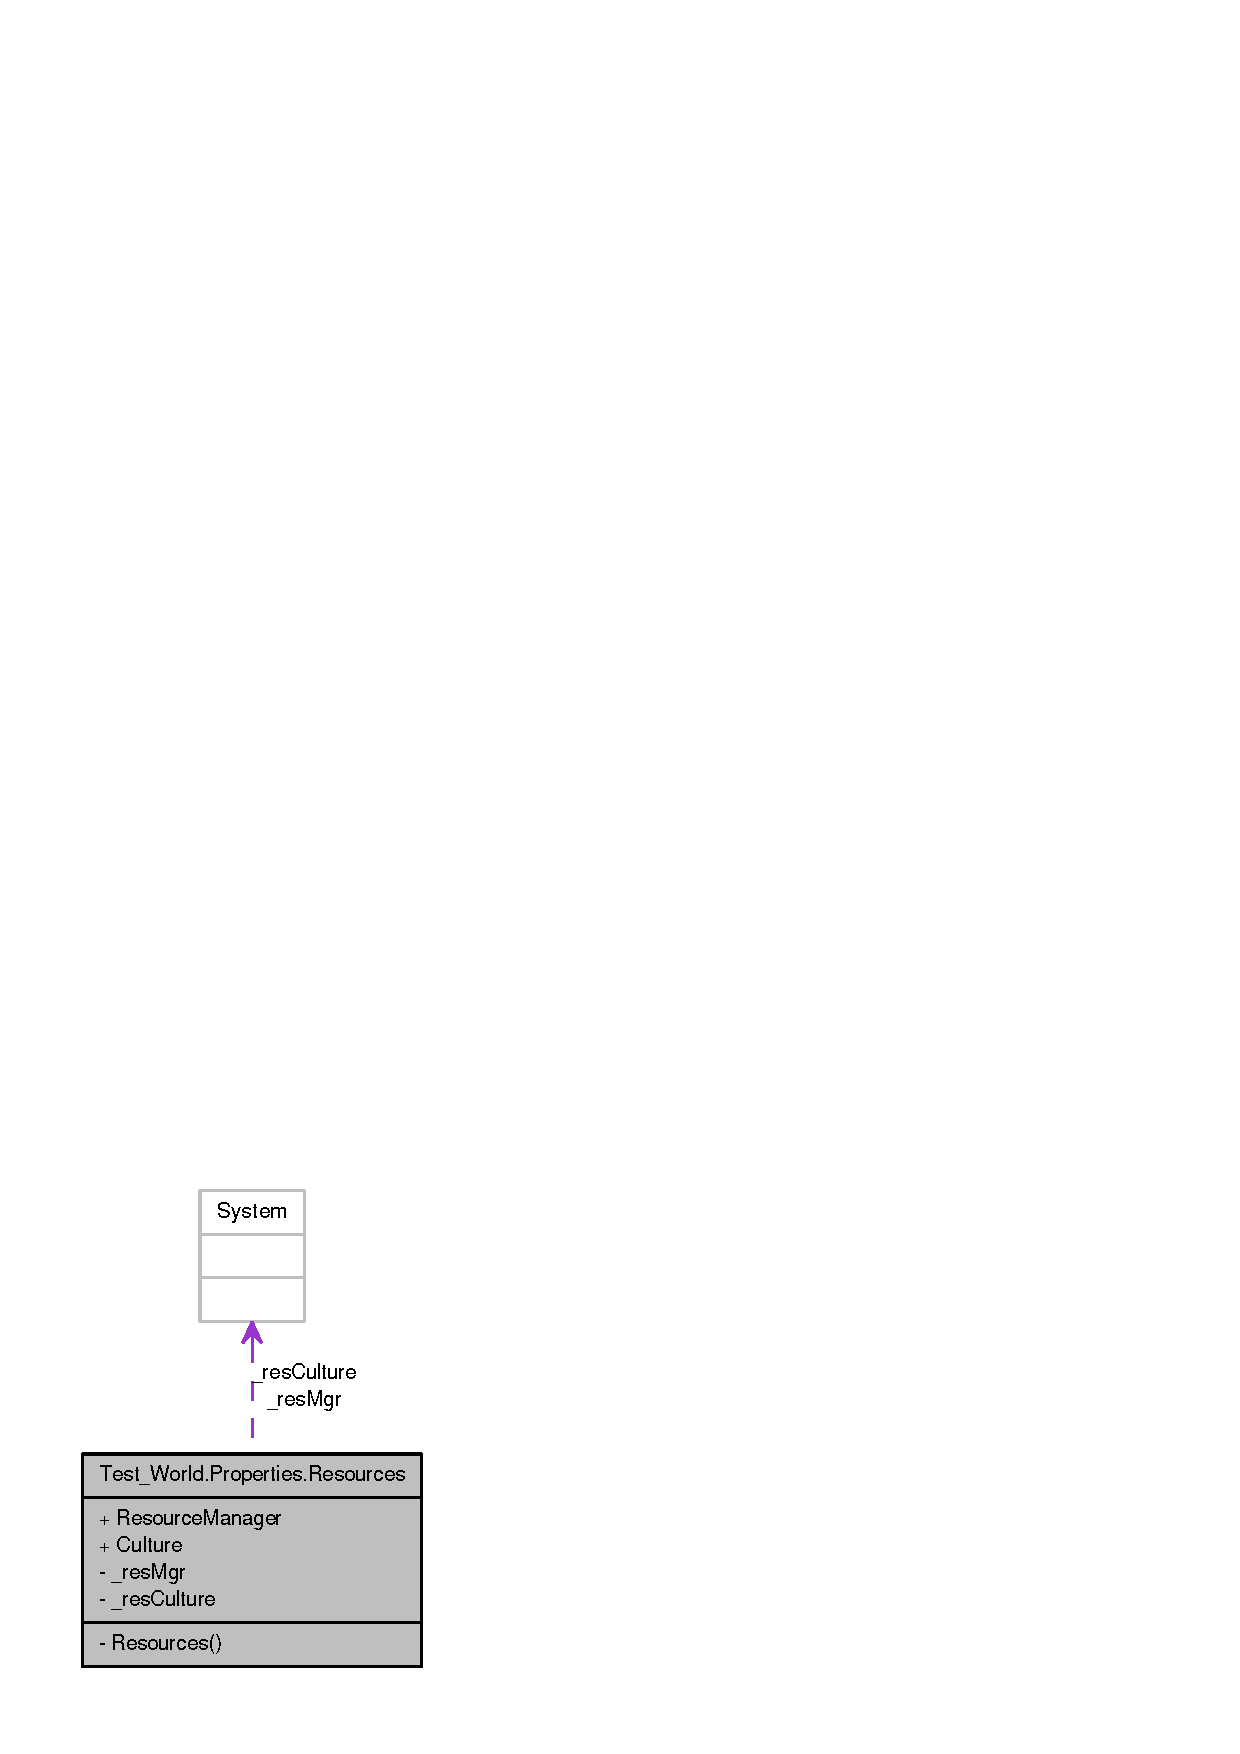
\includegraphics[width=206pt]{class_test___world_1_1_properties_1_1_resources__coll__graph}
\end{center}
\end{figure}
\subsection*{Propertys}
\begin{DoxyCompactItemize}
\item 
static System.Resources.ResourceManager \hyperlink{class_test___world_1_1_properties_1_1_resources_a53b3f19f3590b7cf48b3bfbf1a343023}{ResourceManager}\hspace{0.3cm}{\ttfamily  \mbox{[}get\mbox{]}}
\begin{DoxyCompactList}\small\item\em Returns the cached ResourceManager instance used by this class. \item\end{DoxyCompactList}\item 
static System.Globalization.CultureInfo \hyperlink{class_test___world_1_1_properties_1_1_resources_acb099bdb9ba9fb469c66df36ce63bd25}{Culture}\hspace{0.3cm}{\ttfamily  \mbox{[}get, set\mbox{]}}
\begin{DoxyCompactList}\small\item\em Overrides the current thread's CurrentUICulture property for all resource lookups using this strongly typed resource class. \item\end{DoxyCompactList}\end{DoxyCompactItemize}


\subsection{Ausführliche Beschreibung}
A strongly-\/typed resource class, for looking up localized strings, etc. 

\subsection{Dokumentation der Propertys}
\hypertarget{class_test___world_1_1_properties_1_1_resources_acb099bdb9ba9fb469c66df36ce63bd25}{
\index{Test\_\-World::Properties::Resources@{Test\_\-World::Properties::Resources}!Culture@{Culture}}
\index{Culture@{Culture}!Test_World::Properties::Resources@{Test\_\-World::Properties::Resources}}
\subsubsection[{Culture}]{\setlength{\rightskip}{0pt plus 5cm}System.Globalization.CultureInfo Test\_\-World.Properties.Resources.Culture\hspace{0.3cm}{\ttfamily  \mbox{[}static, get, set\mbox{]}}}}
\label{class_test___world_1_1_properties_1_1_resources_acb099bdb9ba9fb469c66df36ce63bd25}


Overrides the current thread's CurrentUICulture property for all resource lookups using this strongly typed resource class. 

\hypertarget{class_test___world_1_1_properties_1_1_resources_a53b3f19f3590b7cf48b3bfbf1a343023}{
\index{Test\_\-World::Properties::Resources@{Test\_\-World::Properties::Resources}!ResourceManager@{ResourceManager}}
\index{ResourceManager@{ResourceManager}!Test_World::Properties::Resources@{Test\_\-World::Properties::Resources}}
\subsubsection[{ResourceManager}]{\setlength{\rightskip}{0pt plus 5cm}System.Resources.ResourceManager Test\_\-World.Properties.Resources.ResourceManager\hspace{0.3cm}{\ttfamily  \mbox{[}static, get\mbox{]}}}}
\label{class_test___world_1_1_properties_1_1_resources_a53b3f19f3590b7cf48b3bfbf1a343023}


Returns the cached ResourceManager instance used by this class. 



Die Dokumentation für diese Klasse wurde erzeugt aufgrund der Datei:\begin{DoxyCompactItemize}
\item 
Test\_\-World/Properties/Resources.Designer.cs\end{DoxyCompactItemize}

\hypertarget{class_test___drive___x_p_1_1_properties_1_1_resources}{
\section{Test\_\-Drive\_\-XP.Properties.Resources Klassenreferenz}
\label{class_test___drive___x_p_1_1_properties_1_1_resources}\index{Test\_\-Drive\_\-XP::Properties::Resources@{Test\_\-Drive\_\-XP::Properties::Resources}}
}


Eine stark typisierte Ressourcenklasse zum Suchen von lokalisierten Zeichenfolgen usw.  




Zusammengehörigkeiten von Test\_\-Drive\_\-XP.Properties.Resources:\nopagebreak
\begin{figure}[H]
\begin{center}
\leavevmode
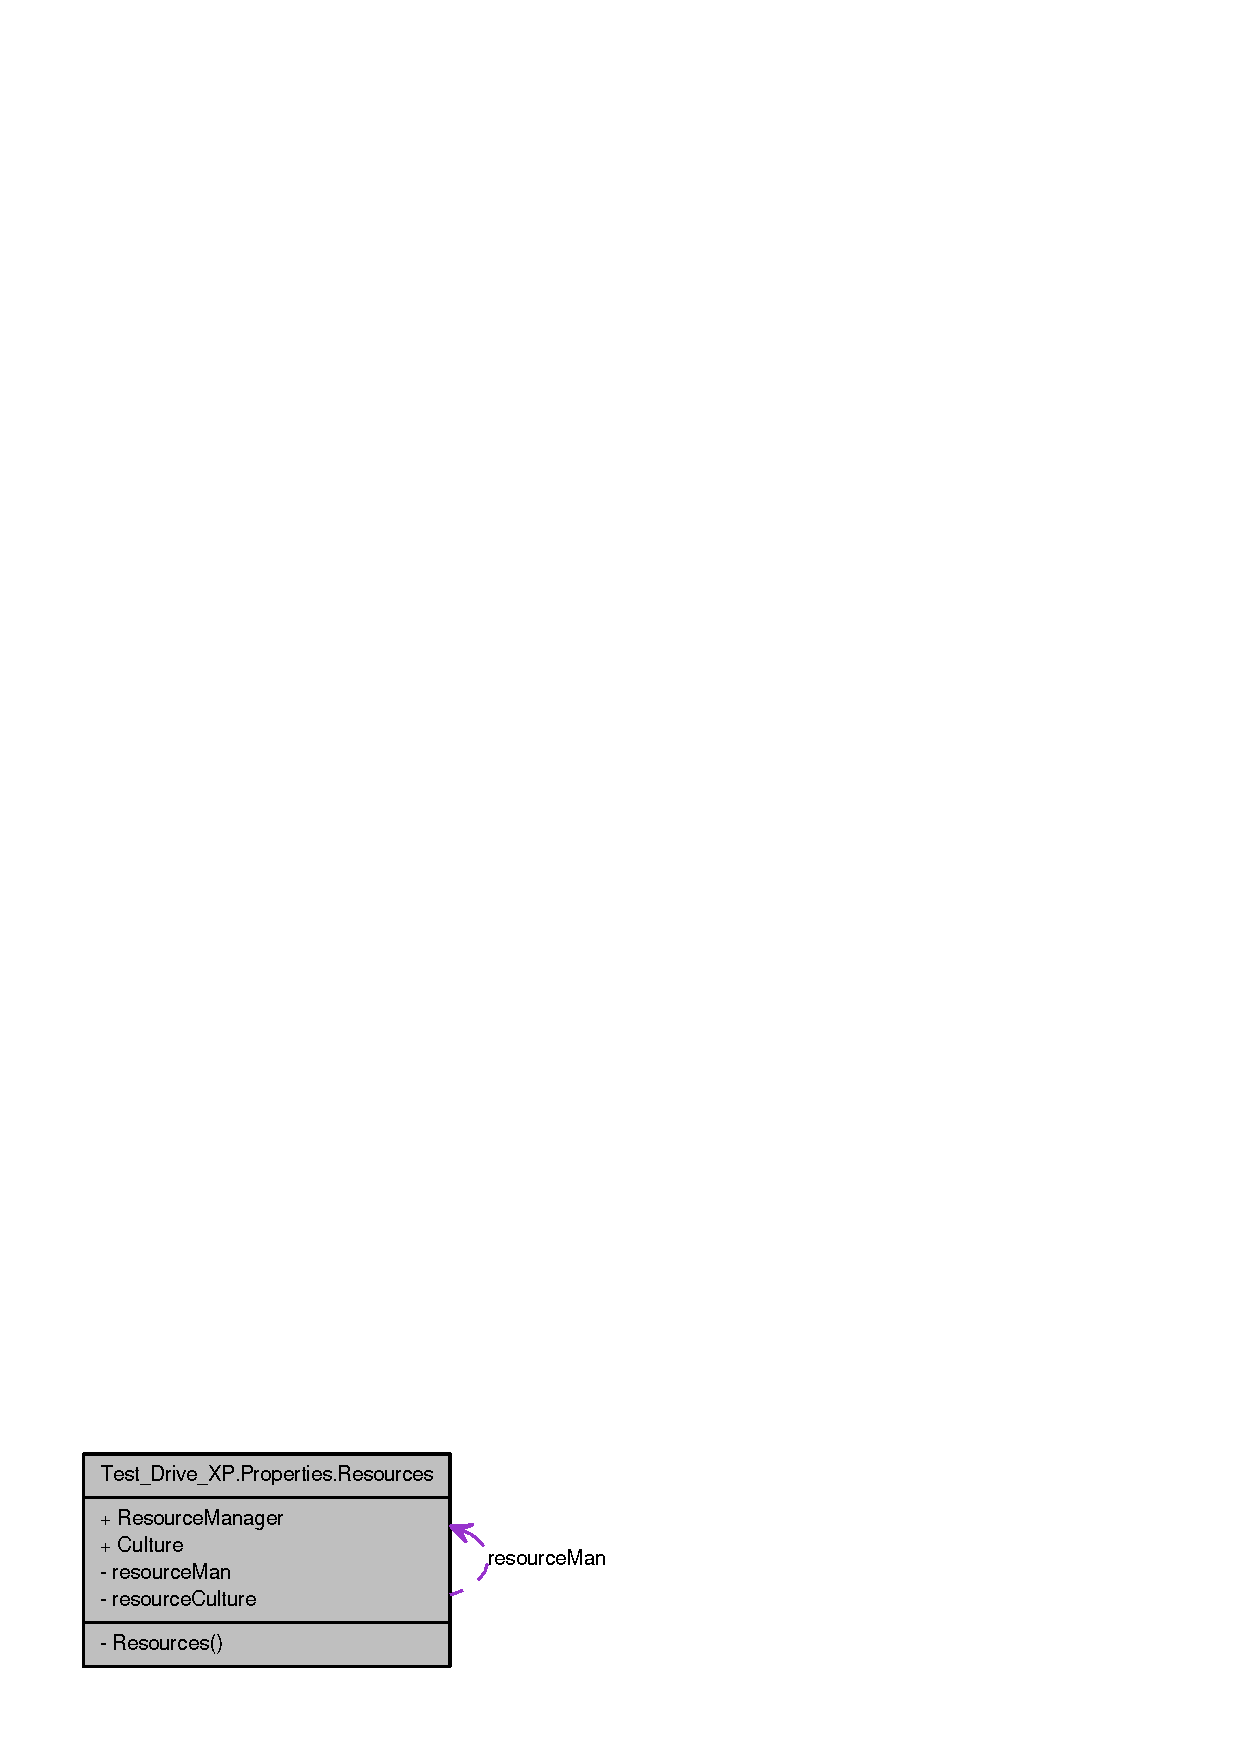
\includegraphics[width=295pt]{class_test___drive___x_p_1_1_properties_1_1_resources__coll__graph}
\end{center}
\end{figure}


\subsection{Ausführliche Beschreibung}
Eine stark typisierte Ressourcenklasse zum Suchen von lokalisierten Zeichenfolgen usw. 

Die Dokumentation für diese Klasse wurde erzeugt aufgrund der Datei:\begin{DoxyCompactItemize}
\item 
Test\_\-Drive\_\-XP/Properties/Resources.Designer.cs\end{DoxyCompactItemize}

\hypertarget{class_test___motor_1_1_properties_1_1_resources}{
\section{Test\_\-Motor.Properties.Resources Klassenreferenz}
\label{class_test___motor_1_1_properties_1_1_resources}\index{Test\_\-Motor::Properties::Resources@{Test\_\-Motor::Properties::Resources}}
}


A strongly-\/typed resource class, for looking up localized strings, etc.  




Zusammengehörigkeiten von Test\_\-Motor.Properties.Resources:\nopagebreak
\begin{figure}[H]
\begin{center}
\leavevmode
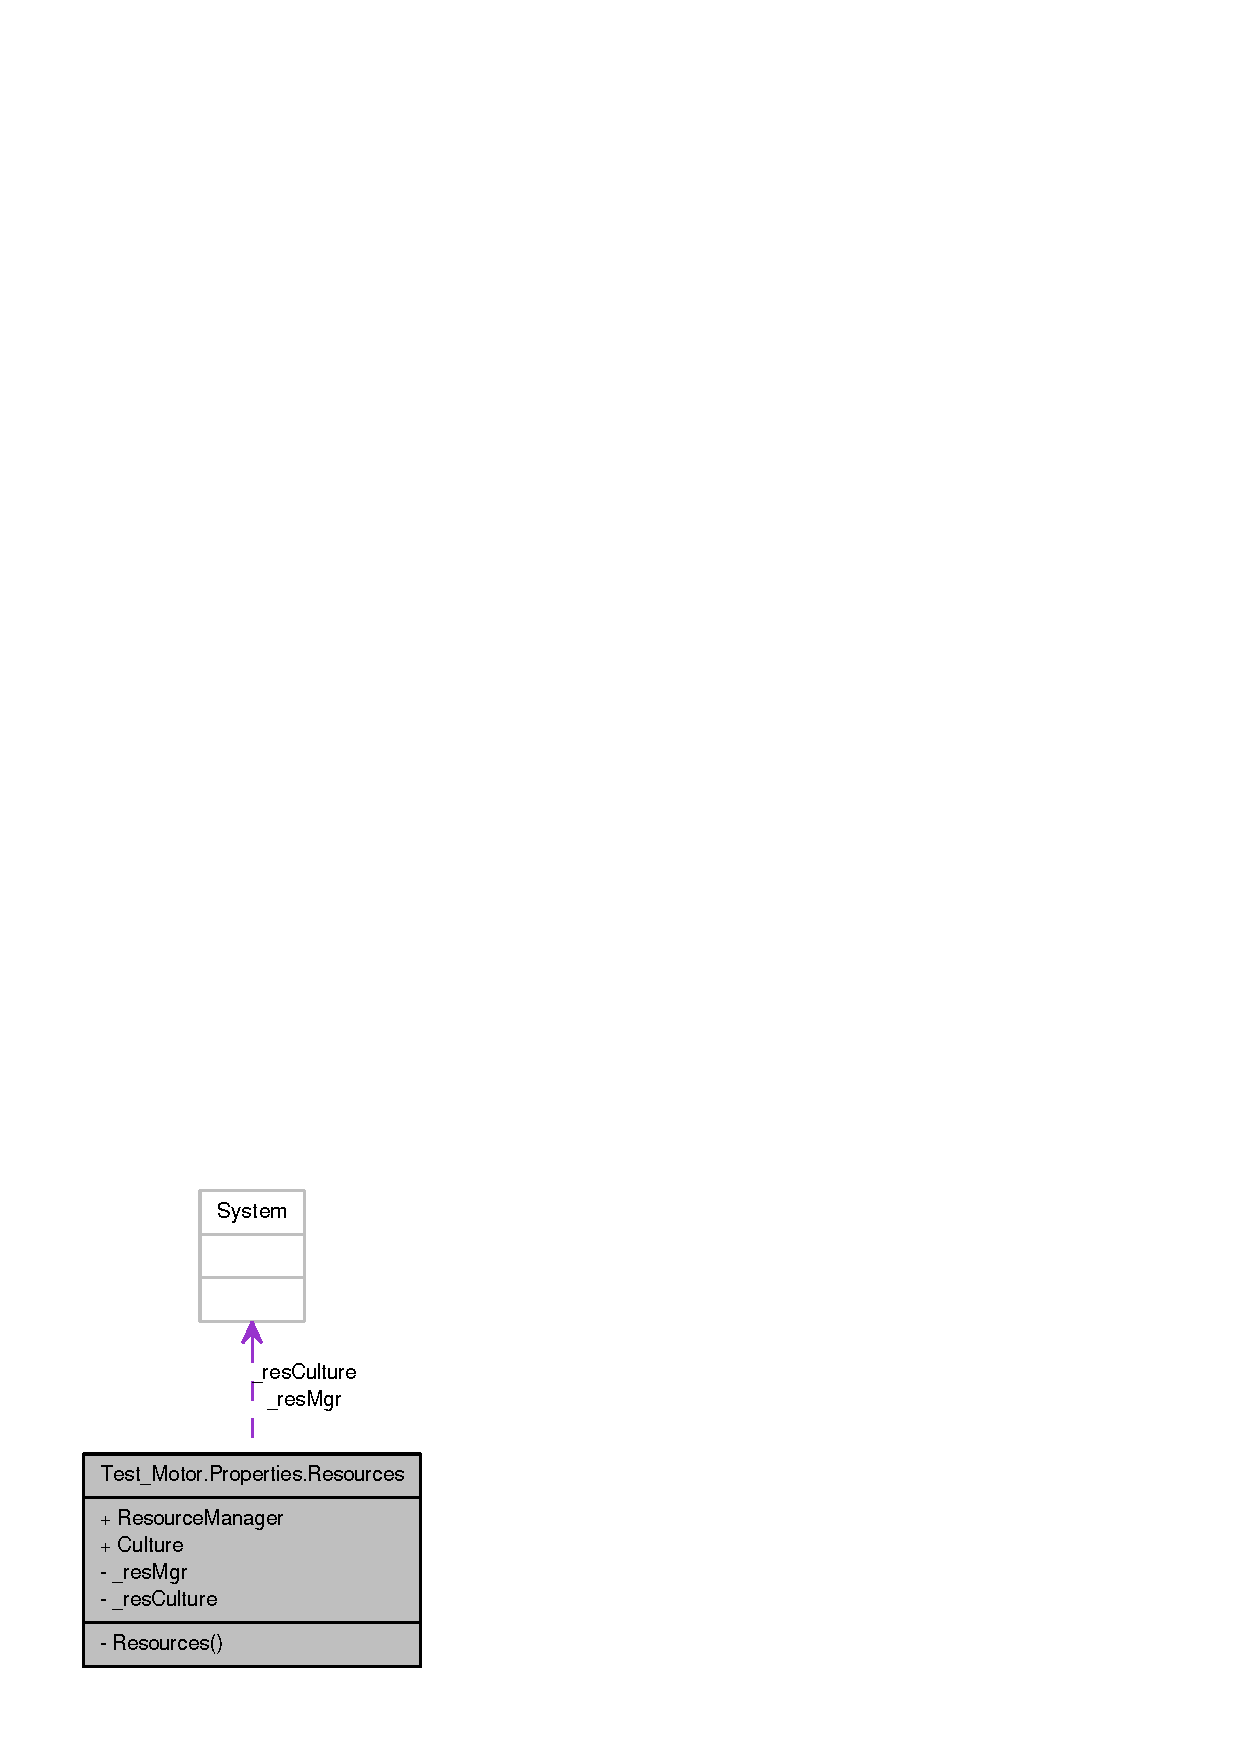
\includegraphics[width=206pt]{class_test___motor_1_1_properties_1_1_resources__coll__graph}
\end{center}
\end{figure}
\subsection*{Propertys}
\begin{DoxyCompactItemize}
\item 
static System.Resources.ResourceManager \hyperlink{class_test___motor_1_1_properties_1_1_resources_a330443da8bc114186360e46f8a44fc01}{ResourceManager}\hspace{0.3cm}{\ttfamily  \mbox{[}get\mbox{]}}
\begin{DoxyCompactList}\small\item\em Returns the cached ResourceManager instance used by this class. \item\end{DoxyCompactList}\item 
static System.Globalization.CultureInfo \hyperlink{class_test___motor_1_1_properties_1_1_resources_ad1c15db40048850de2e5b617b5a56403}{Culture}\hspace{0.3cm}{\ttfamily  \mbox{[}get, set\mbox{]}}
\begin{DoxyCompactList}\small\item\em Overrides the current thread's CurrentUICulture property for all resource lookups using this strongly typed resource class. \item\end{DoxyCompactList}\end{DoxyCompactItemize}


\subsection{Ausführliche Beschreibung}
A strongly-\/typed resource class, for looking up localized strings, etc. 

\subsection{Dokumentation der Propertys}
\hypertarget{class_test___motor_1_1_properties_1_1_resources_ad1c15db40048850de2e5b617b5a56403}{
\index{Test\_\-Motor::Properties::Resources@{Test\_\-Motor::Properties::Resources}!Culture@{Culture}}
\index{Culture@{Culture}!Test_Motor::Properties::Resources@{Test\_\-Motor::Properties::Resources}}
\subsubsection[{Culture}]{\setlength{\rightskip}{0pt plus 5cm}System.Globalization.CultureInfo Test\_\-Motor.Properties.Resources.Culture\hspace{0.3cm}{\ttfamily  \mbox{[}static, get, set\mbox{]}}}}
\label{class_test___motor_1_1_properties_1_1_resources_ad1c15db40048850de2e5b617b5a56403}


Overrides the current thread's CurrentUICulture property for all resource lookups using this strongly typed resource class. 

\hypertarget{class_test___motor_1_1_properties_1_1_resources_a330443da8bc114186360e46f8a44fc01}{
\index{Test\_\-Motor::Properties::Resources@{Test\_\-Motor::Properties::Resources}!ResourceManager@{ResourceManager}}
\index{ResourceManager@{ResourceManager}!Test_Motor::Properties::Resources@{Test\_\-Motor::Properties::Resources}}
\subsubsection[{ResourceManager}]{\setlength{\rightskip}{0pt plus 5cm}System.Resources.ResourceManager Test\_\-Motor.Properties.Resources.ResourceManager\hspace{0.3cm}{\ttfamily  \mbox{[}static, get\mbox{]}}}}
\label{class_test___motor_1_1_properties_1_1_resources_a330443da8bc114186360e46f8a44fc01}


Returns the cached ResourceManager instance used by this class. 



Die Dokumentation für diese Klasse wurde erzeugt aufgrund der Datei:\begin{DoxyCompactItemize}
\item 
Test\_\-Motor\_\-CE/Properties/Resources.Designer.cs\end{DoxyCompactItemize}

\hypertarget{class_test___x_p_1_1_properties_1_1_resources}{
\section{Test\_\-XP.Properties.Resources Klassenreferenz}
\label{class_test___x_p_1_1_properties_1_1_resources}\index{Test\_\-XP::Properties::Resources@{Test\_\-XP::Properties::Resources}}
}


Eine stark typisierte Ressourcenklasse zum Suchen von lokalisierten Zeichenfolgen usw.  




Zusammengehörigkeiten von Test\_\-XP.Properties.Resources:\nopagebreak
\begin{figure}[H]
\begin{center}
\leavevmode
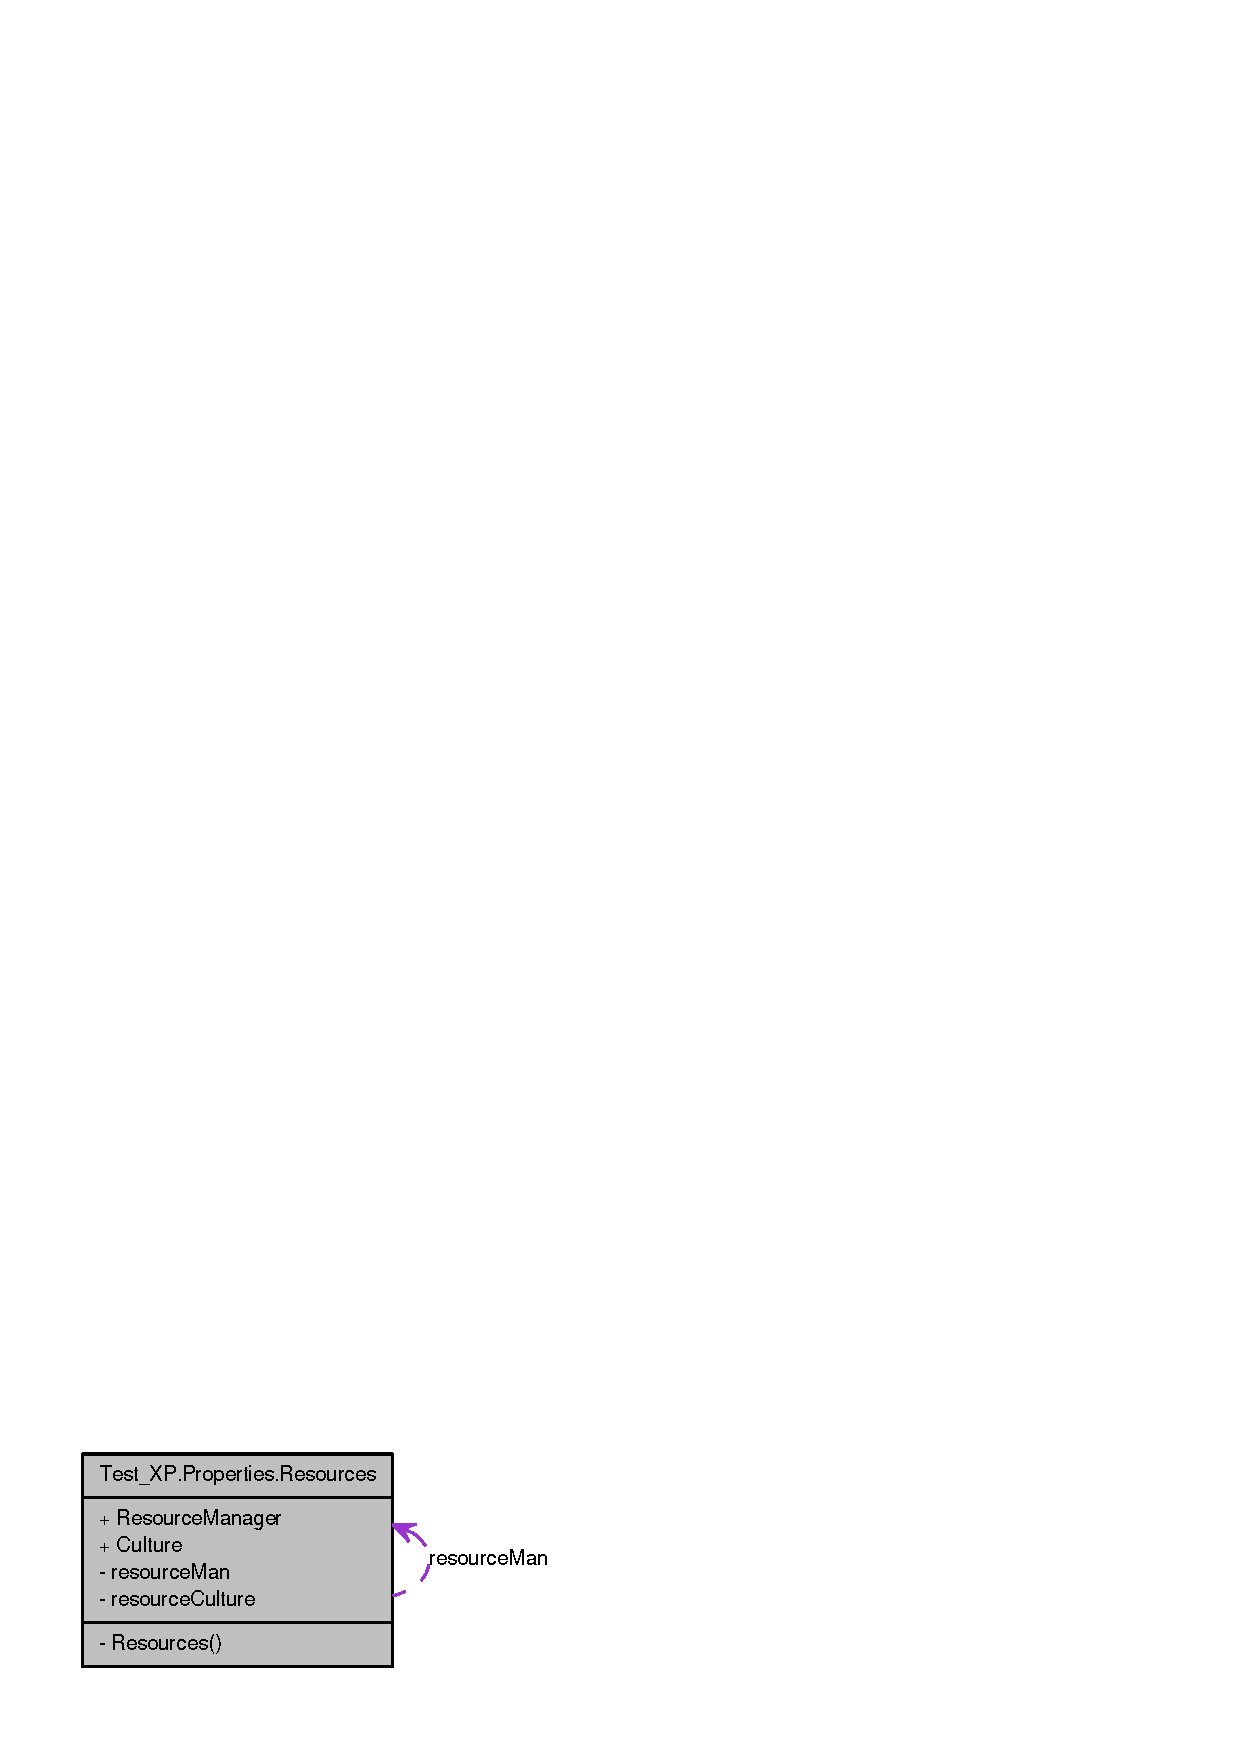
\includegraphics[width=267pt]{class_test___x_p_1_1_properties_1_1_resources__coll__graph}
\end{center}
\end{figure}


\subsection{Ausführliche Beschreibung}
Eine stark typisierte Ressourcenklasse zum Suchen von lokalisierten Zeichenfolgen usw. 

Die Dokumentation für diese Klasse wurde erzeugt aufgrund der Datei:\begin{DoxyCompactItemize}
\item 
Test\_\-XP/Properties/Resources.Designer.cs\end{DoxyCompactItemize}

\hypertarget{class_test___lamp_view_1_1_properties_1_1_resources}{
\section{Test\_\-LampView.Properties.Resources Klassenreferenz}
\label{class_test___lamp_view_1_1_properties_1_1_resources}\index{Test\_\-LampView::Properties::Resources@{Test\_\-LampView::Properties::Resources}}
}


Eine stark typisierte Ressourcenklasse zum Suchen von lokalisierten Zeichenfolgen usw.  




Zusammengehörigkeiten von Test\_\-LampView.Properties.Resources:\nopagebreak
\begin{figure}[H]
\begin{center}
\leavevmode
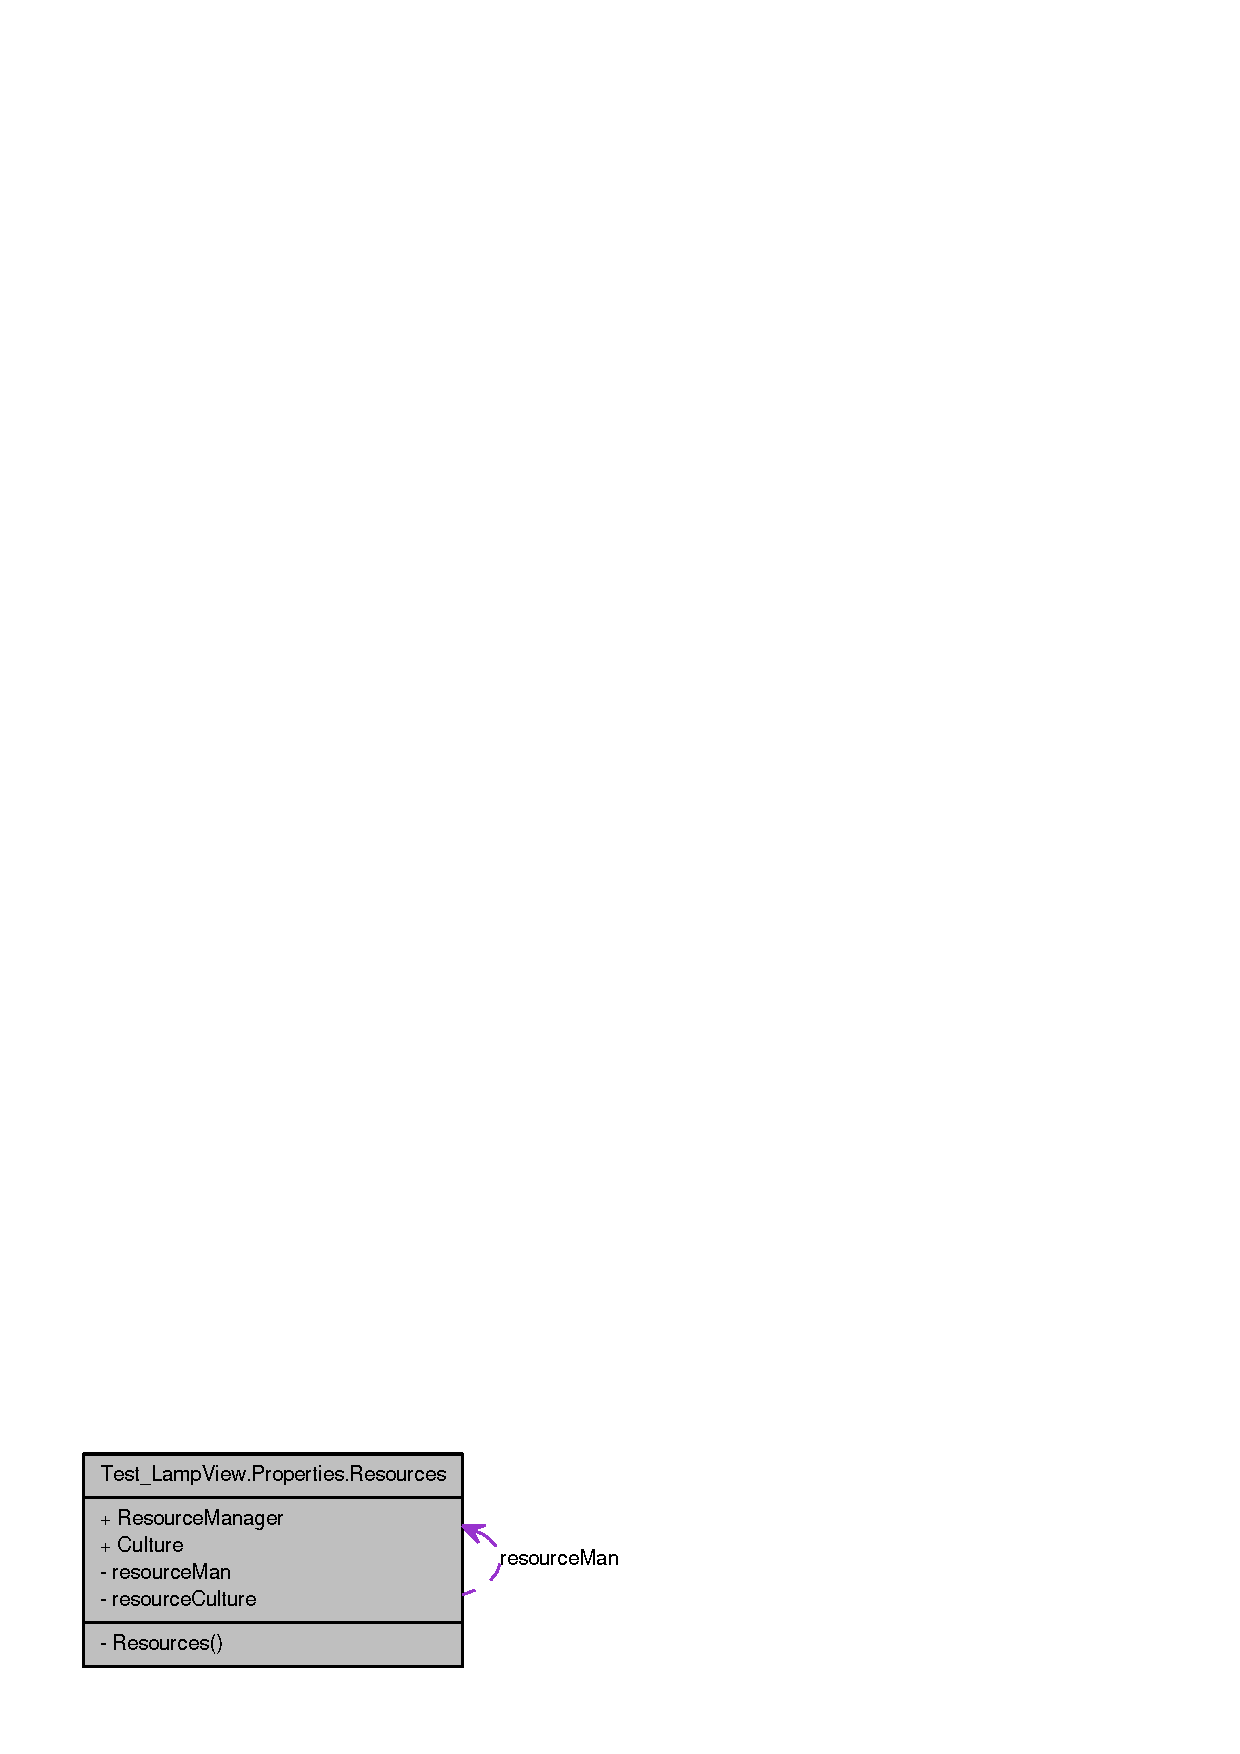
\includegraphics[width=301pt]{class_test___lamp_view_1_1_properties_1_1_resources__coll__graph}
\end{center}
\end{figure}


\subsection{Ausführliche Beschreibung}
Eine stark typisierte Ressourcenklasse zum Suchen von lokalisierten Zeichenfolgen usw. 

Die Dokumentation für diese Klasse wurde erzeugt aufgrund der Datei:\begin{DoxyCompactItemize}
\item 
Test-\/LampView/Properties/Resources.Designer.cs\end{DoxyCompactItemize}

\hypertarget{class_test___c_e_1_1_properties_1_1_resources}{
\section{Test\_\-CE.Properties.Resources Klassenreferenz}
\label{class_test___c_e_1_1_properties_1_1_resources}\index{Test\_\-CE::Properties::Resources@{Test\_\-CE::Properties::Resources}}
}


A strongly-\/typed resource class, for looking up localized strings, etc.  




Zusammengehörigkeiten von Test\_\-CE.Properties.Resources:\nopagebreak
\begin{figure}[H]
\begin{center}
\leavevmode
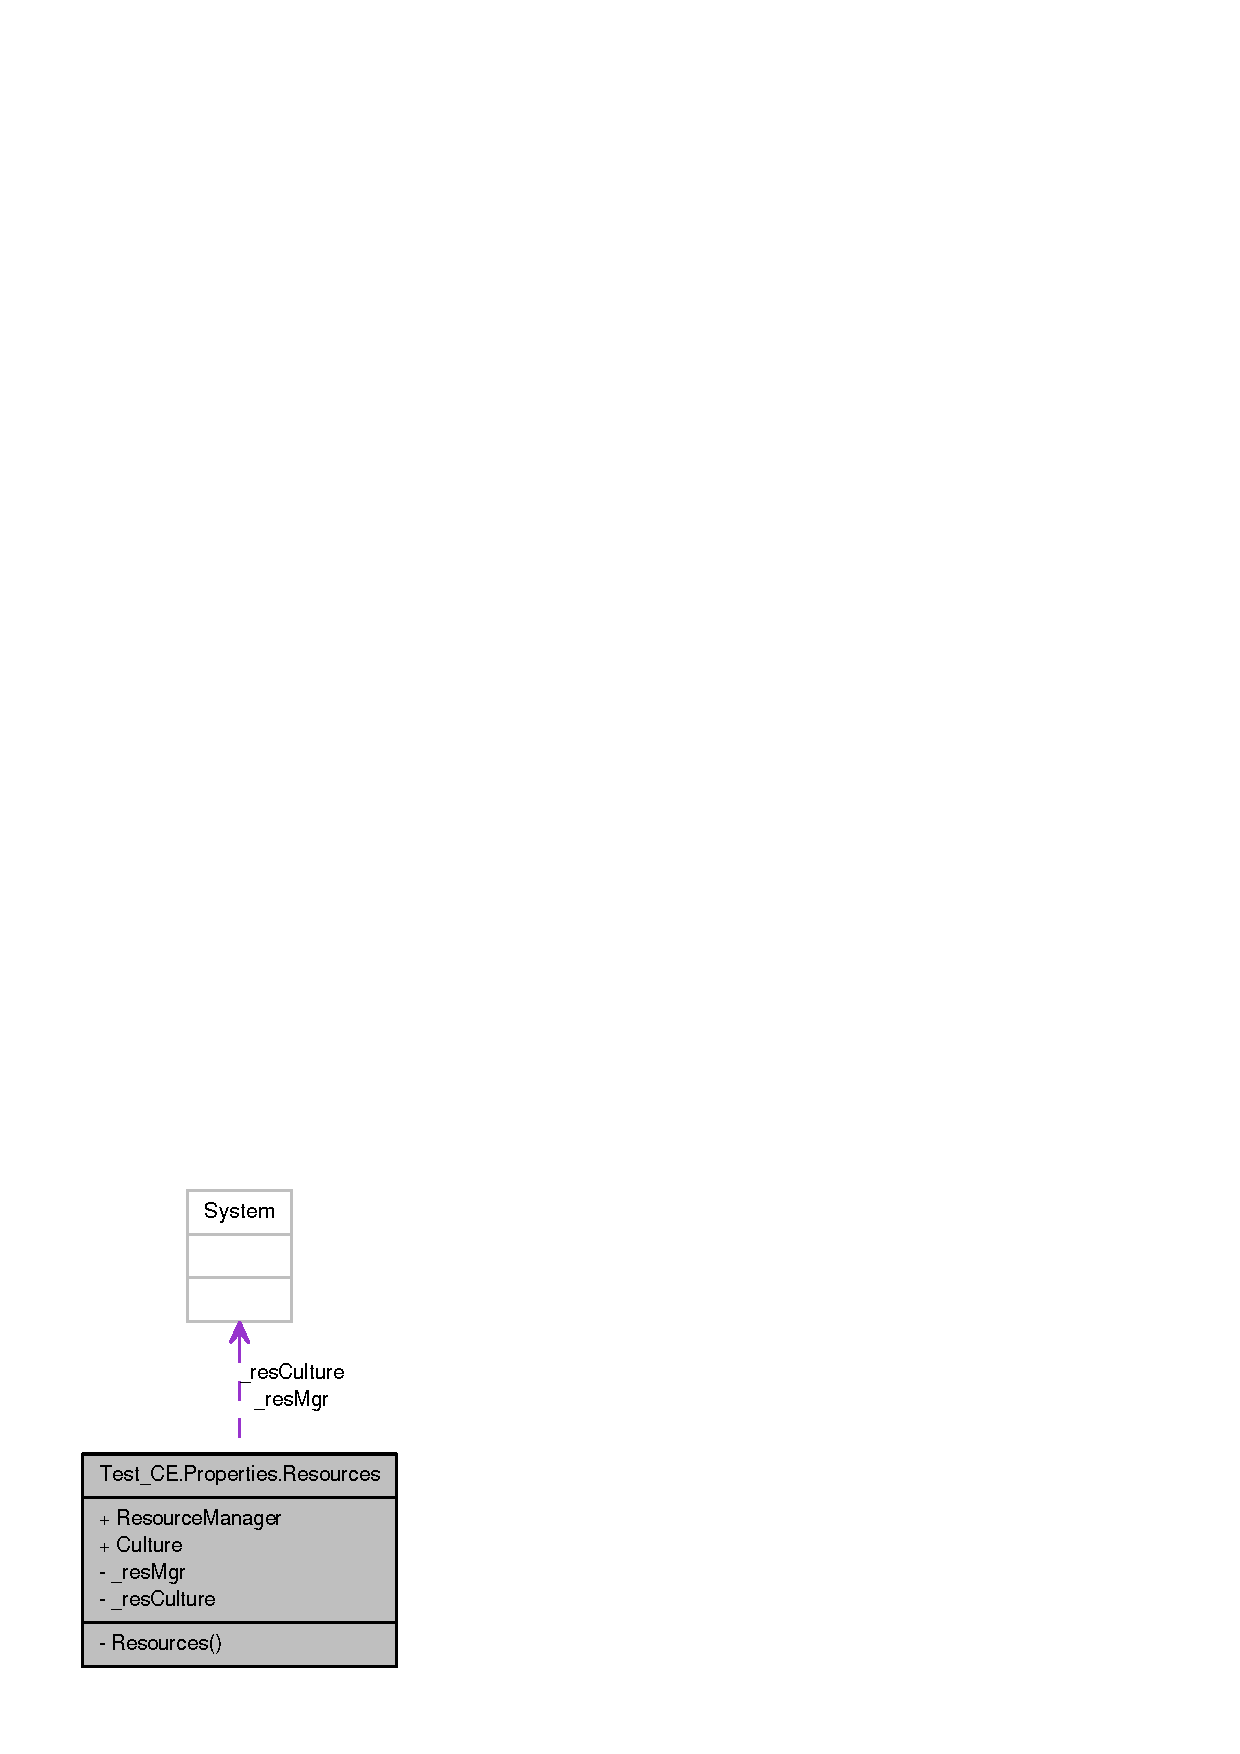
\includegraphics[width=194pt]{class_test___c_e_1_1_properties_1_1_resources__coll__graph}
\end{center}
\end{figure}
\subsection*{Propertys}
\begin{DoxyCompactItemize}
\item 
static System.Resources.ResourceManager \hyperlink{class_test___c_e_1_1_properties_1_1_resources_a34fefe776becc85e7ae843785ef10db7}{ResourceManager}\hspace{0.3cm}{\ttfamily  \mbox{[}get\mbox{]}}
\begin{DoxyCompactList}\small\item\em Returns the cached ResourceManager instance used by this class. \item\end{DoxyCompactList}\item 
static System.Globalization.CultureInfo \hyperlink{class_test___c_e_1_1_properties_1_1_resources_a1721d23c918508899f46aaf22048fefd}{Culture}\hspace{0.3cm}{\ttfamily  \mbox{[}get, set\mbox{]}}
\begin{DoxyCompactList}\small\item\em Overrides the current thread's CurrentUICulture property for all resource lookups using this strongly typed resource class. \item\end{DoxyCompactList}\end{DoxyCompactItemize}


\subsection{Ausführliche Beschreibung}
A strongly-\/typed resource class, for looking up localized strings, etc. 

\subsection{Dokumentation der Propertys}
\hypertarget{class_test___c_e_1_1_properties_1_1_resources_a1721d23c918508899f46aaf22048fefd}{
\index{Test\_\-CE::Properties::Resources@{Test\_\-CE::Properties::Resources}!Culture@{Culture}}
\index{Culture@{Culture}!Test_CE::Properties::Resources@{Test\_\-CE::Properties::Resources}}
\subsubsection[{Culture}]{\setlength{\rightskip}{0pt plus 5cm}System.Globalization.CultureInfo Test\_\-CE.Properties.Resources.Culture\hspace{0.3cm}{\ttfamily  \mbox{[}static, get, set\mbox{]}}}}
\label{class_test___c_e_1_1_properties_1_1_resources_a1721d23c918508899f46aaf22048fefd}


Overrides the current thread's CurrentUICulture property for all resource lookups using this strongly typed resource class. 

\hypertarget{class_test___c_e_1_1_properties_1_1_resources_a34fefe776becc85e7ae843785ef10db7}{
\index{Test\_\-CE::Properties::Resources@{Test\_\-CE::Properties::Resources}!ResourceManager@{ResourceManager}}
\index{ResourceManager@{ResourceManager}!Test_CE::Properties::Resources@{Test\_\-CE::Properties::Resources}}
\subsubsection[{ResourceManager}]{\setlength{\rightskip}{0pt plus 5cm}System.Resources.ResourceManager Test\_\-CE.Properties.Resources.ResourceManager\hspace{0.3cm}{\ttfamily  \mbox{[}static, get\mbox{]}}}}
\label{class_test___c_e_1_1_properties_1_1_resources_a34fefe776becc85e7ae843785ef10db7}


Returns the cached ResourceManager instance used by this class. 



Die Dokumentation für diese Klasse wurde erzeugt aufgrund der Datei:\begin{DoxyCompactItemize}
\item 
Test\_\-CE/Properties/Resources.Designer.cs\end{DoxyCompactItemize}

\hypertarget{class_test___drive___c_e_1_1_properties_1_1_resources}{
\section{Test\_\-Drive\_\-CE.Properties.Resources Klassenreferenz}
\label{class_test___drive___c_e_1_1_properties_1_1_resources}\index{Test\_\-Drive\_\-CE::Properties::Resources@{Test\_\-Drive\_\-CE::Properties::Resources}}
}


A strongly-\/typed resource class, for looking up localized strings, etc.  




Zusammengehörigkeiten von Test\_\-Drive\_\-CE.Properties.Resources:\nopagebreak
\begin{figure}[H]
\begin{center}
\leavevmode
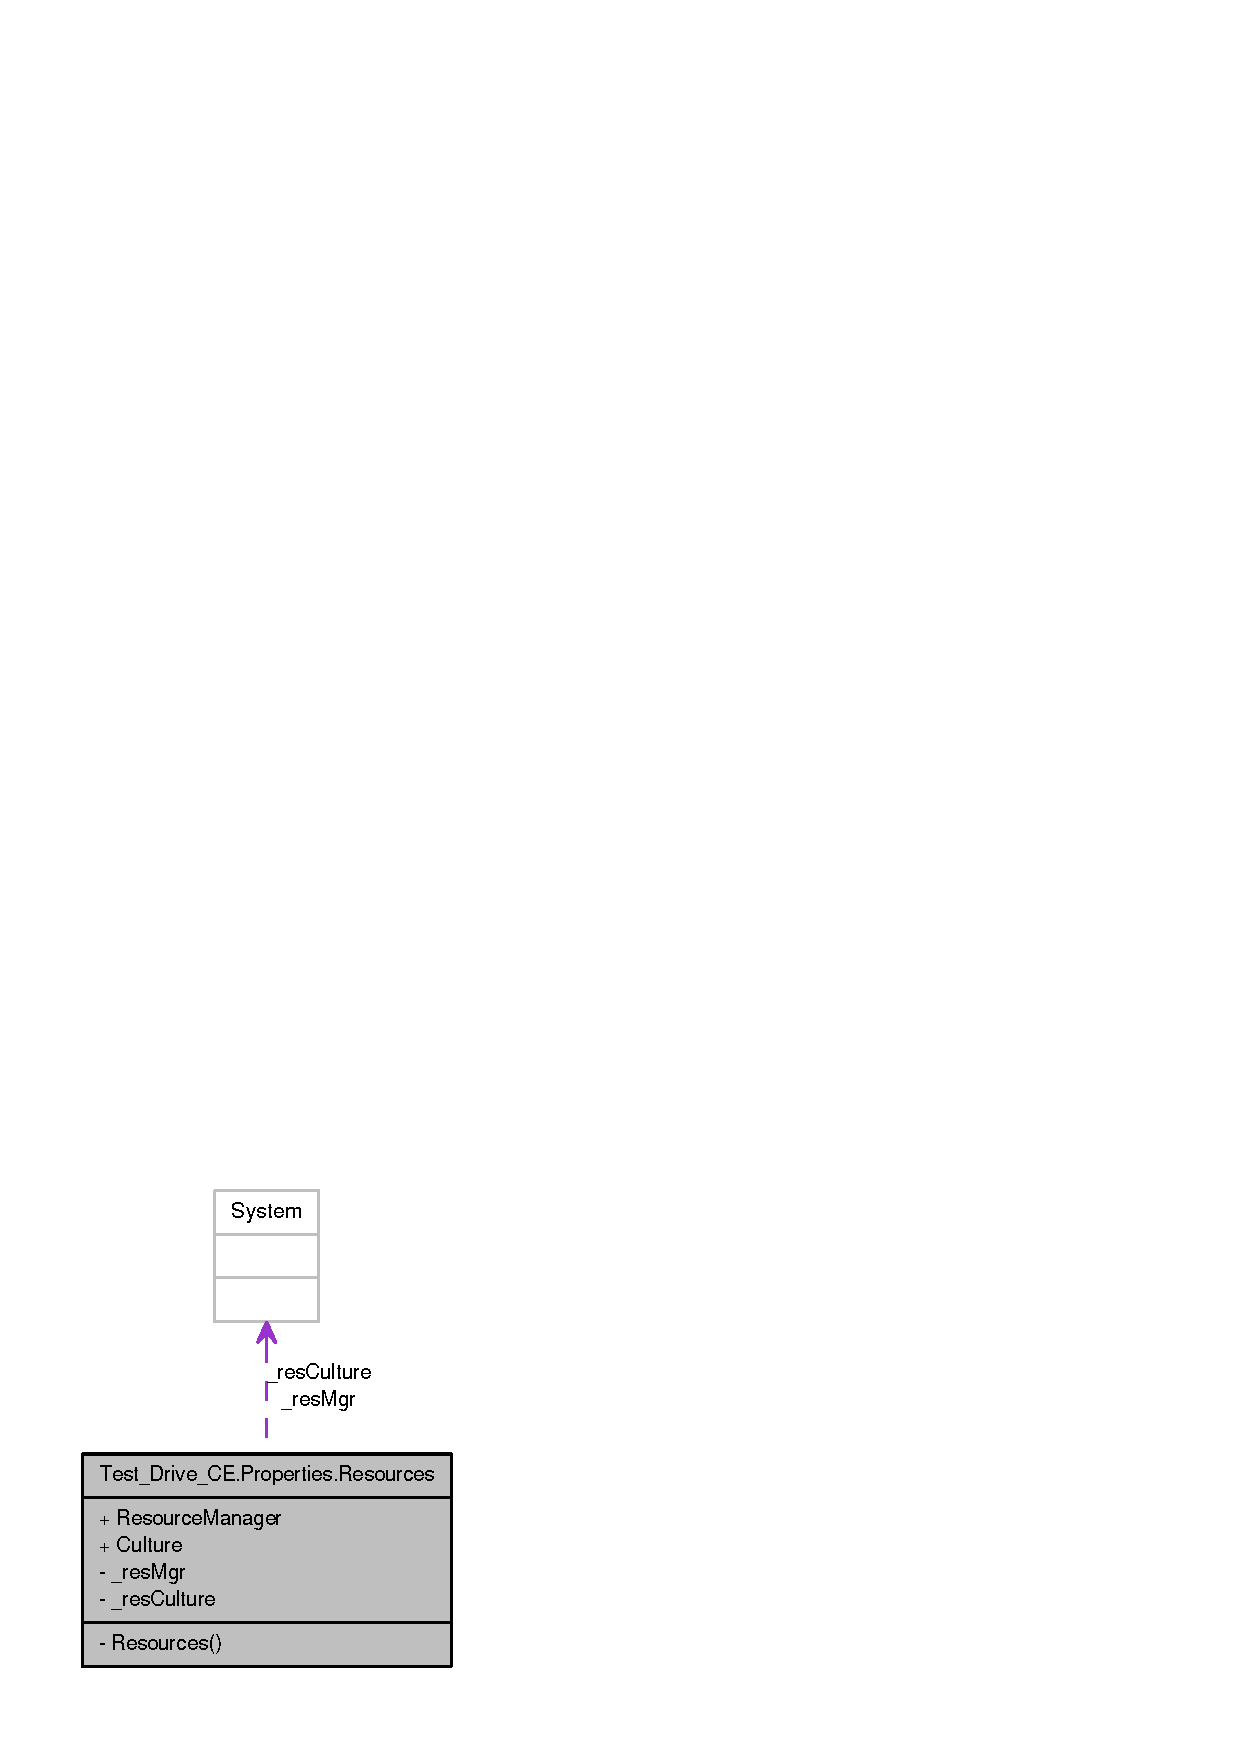
\includegraphics[width=220pt]{class_test___drive___c_e_1_1_properties_1_1_resources__coll__graph}
\end{center}
\end{figure}
\subsection*{Propertys}
\begin{DoxyCompactItemize}
\item 
static System.Resources.ResourceManager \hyperlink{class_test___drive___c_e_1_1_properties_1_1_resources_a97da4c165bc96ab20ba9775fd55be717}{ResourceManager}\hspace{0.3cm}{\ttfamily  \mbox{[}get\mbox{]}}
\begin{DoxyCompactList}\small\item\em Returns the cached ResourceManager instance used by this class. \item\end{DoxyCompactList}\item 
static System.Globalization.CultureInfo \hyperlink{class_test___drive___c_e_1_1_properties_1_1_resources_ad2ae1b65b5936fb3c18c099fdfc58380}{Culture}\hspace{0.3cm}{\ttfamily  \mbox{[}get, set\mbox{]}}
\begin{DoxyCompactList}\small\item\em Overrides the current thread's CurrentUICulture property for all resource lookups using this strongly typed resource class. \item\end{DoxyCompactList}\end{DoxyCompactItemize}


\subsection{Ausführliche Beschreibung}
A strongly-\/typed resource class, for looking up localized strings, etc. 

\subsection{Dokumentation der Propertys}
\hypertarget{class_test___drive___c_e_1_1_properties_1_1_resources_ad2ae1b65b5936fb3c18c099fdfc58380}{
\index{Test\_\-Drive\_\-CE::Properties::Resources@{Test\_\-Drive\_\-CE::Properties::Resources}!Culture@{Culture}}
\index{Culture@{Culture}!Test_Drive_CE::Properties::Resources@{Test\_\-Drive\_\-CE::Properties::Resources}}
\subsubsection[{Culture}]{\setlength{\rightskip}{0pt plus 5cm}System.Globalization.CultureInfo Test\_\-Drive\_\-CE.Properties.Resources.Culture\hspace{0.3cm}{\ttfamily  \mbox{[}static, get, set\mbox{]}}}}
\label{class_test___drive___c_e_1_1_properties_1_1_resources_ad2ae1b65b5936fb3c18c099fdfc58380}


Overrides the current thread's CurrentUICulture property for all resource lookups using this strongly typed resource class. 

\hypertarget{class_test___drive___c_e_1_1_properties_1_1_resources_a97da4c165bc96ab20ba9775fd55be717}{
\index{Test\_\-Drive\_\-CE::Properties::Resources@{Test\_\-Drive\_\-CE::Properties::Resources}!ResourceManager@{ResourceManager}}
\index{ResourceManager@{ResourceManager}!Test_Drive_CE::Properties::Resources@{Test\_\-Drive\_\-CE::Properties::Resources}}
\subsubsection[{ResourceManager}]{\setlength{\rightskip}{0pt plus 5cm}System.Resources.ResourceManager Test\_\-Drive\_\-CE.Properties.Resources.ResourceManager\hspace{0.3cm}{\ttfamily  \mbox{[}static, get\mbox{]}}}}
\label{class_test___drive___c_e_1_1_properties_1_1_resources_a97da4c165bc96ab20ba9775fd55be717}


Returns the cached ResourceManager instance used by this class. 



Die Dokumentation für diese Klasse wurde erzeugt aufgrund der Datei:\begin{DoxyCompactItemize}
\item 
Test\_\-Drive\_\-CE/Properties/Resources.Designer.cs\end{DoxyCompactItemize}

\hypertarget{class_test___motor___x_p_1_1_properties_1_1_resources}{
\section{Test\_\-Motor\_\-XP.Properties.Resources Klassenreferenz}
\label{class_test___motor___x_p_1_1_properties_1_1_resources}\index{Test\_\-Motor\_\-XP::Properties::Resources@{Test\_\-Motor\_\-XP::Properties::Resources}}
}


Eine stark typisierte Ressourcenklasse zum Suchen von lokalisierten Zeichenfolgen usw.  




Zusammengehörigkeiten von Test\_\-Motor\_\-XP.Properties.Resources:\nopagebreak
\begin{figure}[H]
\begin{center}
\leavevmode
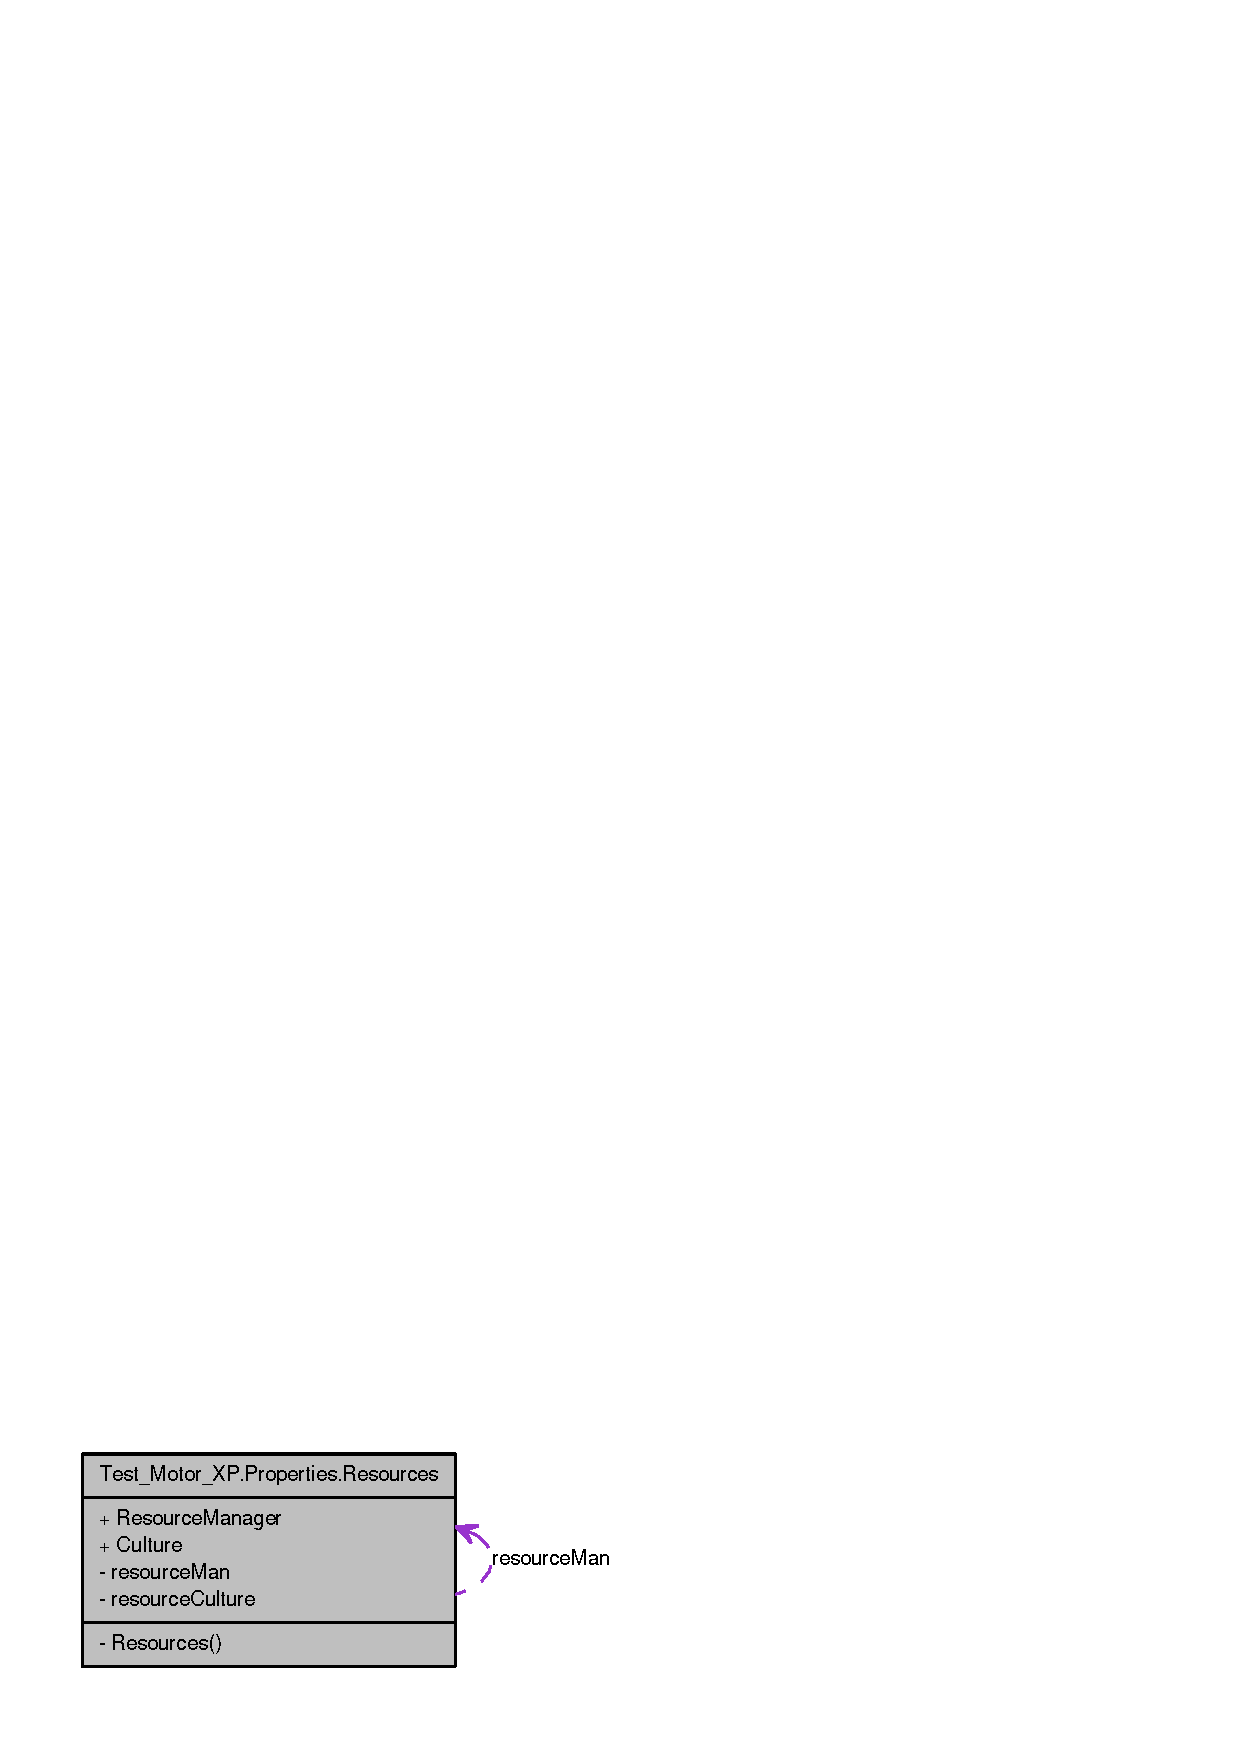
\includegraphics[width=297pt]{class_test___motor___x_p_1_1_properties_1_1_resources__coll__graph}
\end{center}
\end{figure}


\subsection{Ausführliche Beschreibung}
Eine stark typisierte Ressourcenklasse zum Suchen von lokalisierten Zeichenfolgen usw. 

Die Dokumentation für diese Klasse wurde erzeugt aufgrund der Datei:\begin{DoxyCompactItemize}
\item 
Test\_\-Motor\_\-XP/Properties/Resources.Designer.cs\end{DoxyCompactItemize}

\hypertarget{class_robot_ctrl_1_1_robot}{
\section{RobotCtrl.Robot Klassenreferenz}
\label{class_robot_ctrl_1_1_robot}\index{RobotCtrl::Robot@{RobotCtrl::Robot}}
}


Basisklasse f\"{u}r einen Roboter.  




Zusammengehörigkeiten von RobotCtrl.Robot:\subsection*{Öffentliche Methoden}
\begin{DoxyCompactItemize}
\item 
\hyperlink{class_robot_ctrl_1_1_robot_acdd921df41328916b058eaad84ed3078}{Robot} (RunMode runMode)
\end{DoxyCompactItemize}
\subsection*{Propertys}
\begin{DoxyCompactItemize}
\item 
\hyperlink{class_robot_ctrl_1_1_console}{Console} \hyperlink{class_robot_ctrl_1_1_robot_ae78d1691cc943383977741712962bf82}{Console}\hspace{0.3cm}{\ttfamily  \mbox{[}get\mbox{]}}
\item 
\hyperlink{class_robot_ctrl_1_1_drive}{Drive} \hyperlink{class_robot_ctrl_1_1_robot_a6e1e59f43f8578d78da6c6a19e55f269}{Drive}\hspace{0.3cm}{\ttfamily  \mbox{[}get\mbox{]}}
\item 
\hyperlink{class_robot_ctrl_1_1_radar}{Radar} \hyperlink{class_robot_ctrl_1_1_robot_adcc563b2531e72dcdfb9af5cafda1cbc}{Radar}\hspace{0.3cm}{\ttfamily  \mbox{[}get\mbox{]}}
\end{DoxyCompactItemize}


\subsection{Ausführliche Beschreibung}
Basisklasse f\"{u}r einen Roboter. Klasse \hyperlink{class_robot_ctrl_1_1_robot}{Robot}, dient als Basis f\"{u}r einen realen oder virtuellen Roboter 

\subsection{Beschreibung der Konstruktoren und Destruktoren}
\hypertarget{class_robot_ctrl_1_1_robot_acdd921df41328916b058eaad84ed3078}{
\index{RobotCtrl::Robot@{RobotCtrl::Robot}!Robot@{Robot}}
\index{Robot@{Robot}!RobotCtrl::Robot@{RobotCtrl::Robot}}
\subsubsection[{Robot}]{\setlength{\rightskip}{0pt plus 5cm}RobotCtrl.Robot.Robot (RunMode {\em runMode})}}
\label{class_robot_ctrl_1_1_robot_acdd921df41328916b058eaad84ed3078}
Konstruktor f\"{u}r die Klasse \hyperlink{class_robot_ctrl_1_1_robot}{Robot} \begin{DoxySeeAlso}{Siehe auch}
RunMode
\end{DoxySeeAlso}

\begin{DoxyParams}{Parameter}
\item[{\em runMode}]argument vom Typ enum RunMode in \hyperlink{class_robot_ctrl_1_1_config}{Config}. \end{DoxyParams}


\subsection{Dokumentation der Propertys}
\hypertarget{class_robot_ctrl_1_1_robot_ae78d1691cc943383977741712962bf82}{
\index{RobotCtrl::Robot@{RobotCtrl::Robot}!Console@{Console}}
\index{Console@{Console}!RobotCtrl::Robot@{RobotCtrl::Robot}}
\subsubsection[{Console}]{\setlength{\rightskip}{0pt plus 5cm}{\bf Console} RobotCtrl.Robot.Console\hspace{0.3cm}{\ttfamily  \mbox{[}get\mbox{]}}}}
\label{class_robot_ctrl_1_1_robot_ae78d1691cc943383977741712962bf82}
Property \hyperlink{class_robot_ctrl_1_1_console}{Console} liefert eine Referenz auf die \hyperlink{class_robot_ctrl_1_1_console}{Console} innerhalb des \hyperlink{class_robot_ctrl_1_1_robot}{Robot} Objektes \begin{DoxySeeAlso}{Siehe auch}
\hyperlink{class_robot_ctrl_1_1_console}{Console}
\end{DoxySeeAlso}
\begin{DoxyReturn}{Rückgabe}
\hyperlink{class_robot_ctrl_1_1_robot}{Robot} \hyperlink{class_robot_ctrl_1_1_console}{Console} 
\end{DoxyReturn}
\hypertarget{class_robot_ctrl_1_1_robot_a6e1e59f43f8578d78da6c6a19e55f269}{
\index{RobotCtrl::Robot@{RobotCtrl::Robot}!Drive@{Drive}}
\index{Drive@{Drive}!RobotCtrl::Robot@{RobotCtrl::Robot}}
\subsubsection[{Drive}]{\setlength{\rightskip}{0pt plus 5cm}{\bf Drive} RobotCtrl.Robot.Drive\hspace{0.3cm}{\ttfamily  \mbox{[}get\mbox{]}}}}
\label{class_robot_ctrl_1_1_robot_a6e1e59f43f8578d78da6c6a19e55f269}
Property \hyperlink{class_robot_ctrl_1_1_drive}{Drive} liefert eine Referenz auf \hyperlink{class_robot_ctrl_1_1_drive}{Drive} innerhalb des \hyperlink{class_robot_ctrl_1_1_robot}{Robot} Objektes \begin{DoxySeeAlso}{Siehe auch}
\hyperlink{class_robot_ctrl_1_1_drive}{Drive}
\end{DoxySeeAlso}
\begin{DoxyReturn}{Rückgabe}
\hyperlink{class_robot_ctrl_1_1_drive}{Drive} f\"{u}r den \hyperlink{class_robot_ctrl_1_1_robot}{Robot} 
\end{DoxyReturn}
\hypertarget{class_robot_ctrl_1_1_robot_adcc563b2531e72dcdfb9af5cafda1cbc}{
\index{RobotCtrl::Robot@{RobotCtrl::Robot}!Radar@{Radar}}
\index{Radar@{Radar}!RobotCtrl::Robot@{RobotCtrl::Robot}}
\subsubsection[{Radar}]{\setlength{\rightskip}{0pt plus 5cm}{\bf Radar} RobotCtrl.Robot.Radar\hspace{0.3cm}{\ttfamily  \mbox{[}get\mbox{]}}}}
\label{class_robot_ctrl_1_1_robot_adcc563b2531e72dcdfb9af5cafda1cbc}
Property \hyperlink{class_robot_ctrl_1_1_radar}{Radar} liefert eine Referenz auf \hyperlink{class_robot_ctrl_1_1_radar}{Radar} innerhalb des \hyperlink{class_robot_ctrl_1_1_robot}{Robot} Objektes \begin{DoxySeeAlso}{Siehe auch}
\hyperlink{class_robot_ctrl_1_1_radar}{Radar}
\end{DoxySeeAlso}
\begin{DoxyReturn}{Rückgabe}
\hyperlink{class_robot_ctrl_1_1_radar}{Radar} f\"{u}r den \hyperlink{class_robot_ctrl_1_1_robot}{Robot} 
\end{DoxyReturn}


Die Dokumentation für diese Klasse wurde erzeugt aufgrund der Datei:\begin{DoxyCompactItemize}
\item 
Robot.cs\end{DoxyCompactItemize}

\hypertarget{class_test___x_p_1_1_properties_1_1_settings}{
\section{Test\_\-XP.Properties.Settings Klassenreferenz}
\label{class_test___x_p_1_1_properties_1_1_settings}\index{Test\_\-XP::Properties::Settings@{Test\_\-XP::Properties::Settings}}
}


Zusammengehörigkeiten von Test\_\-XP.Properties.Settings:\nopagebreak
\begin{figure}[H]
\begin{center}
\leavevmode
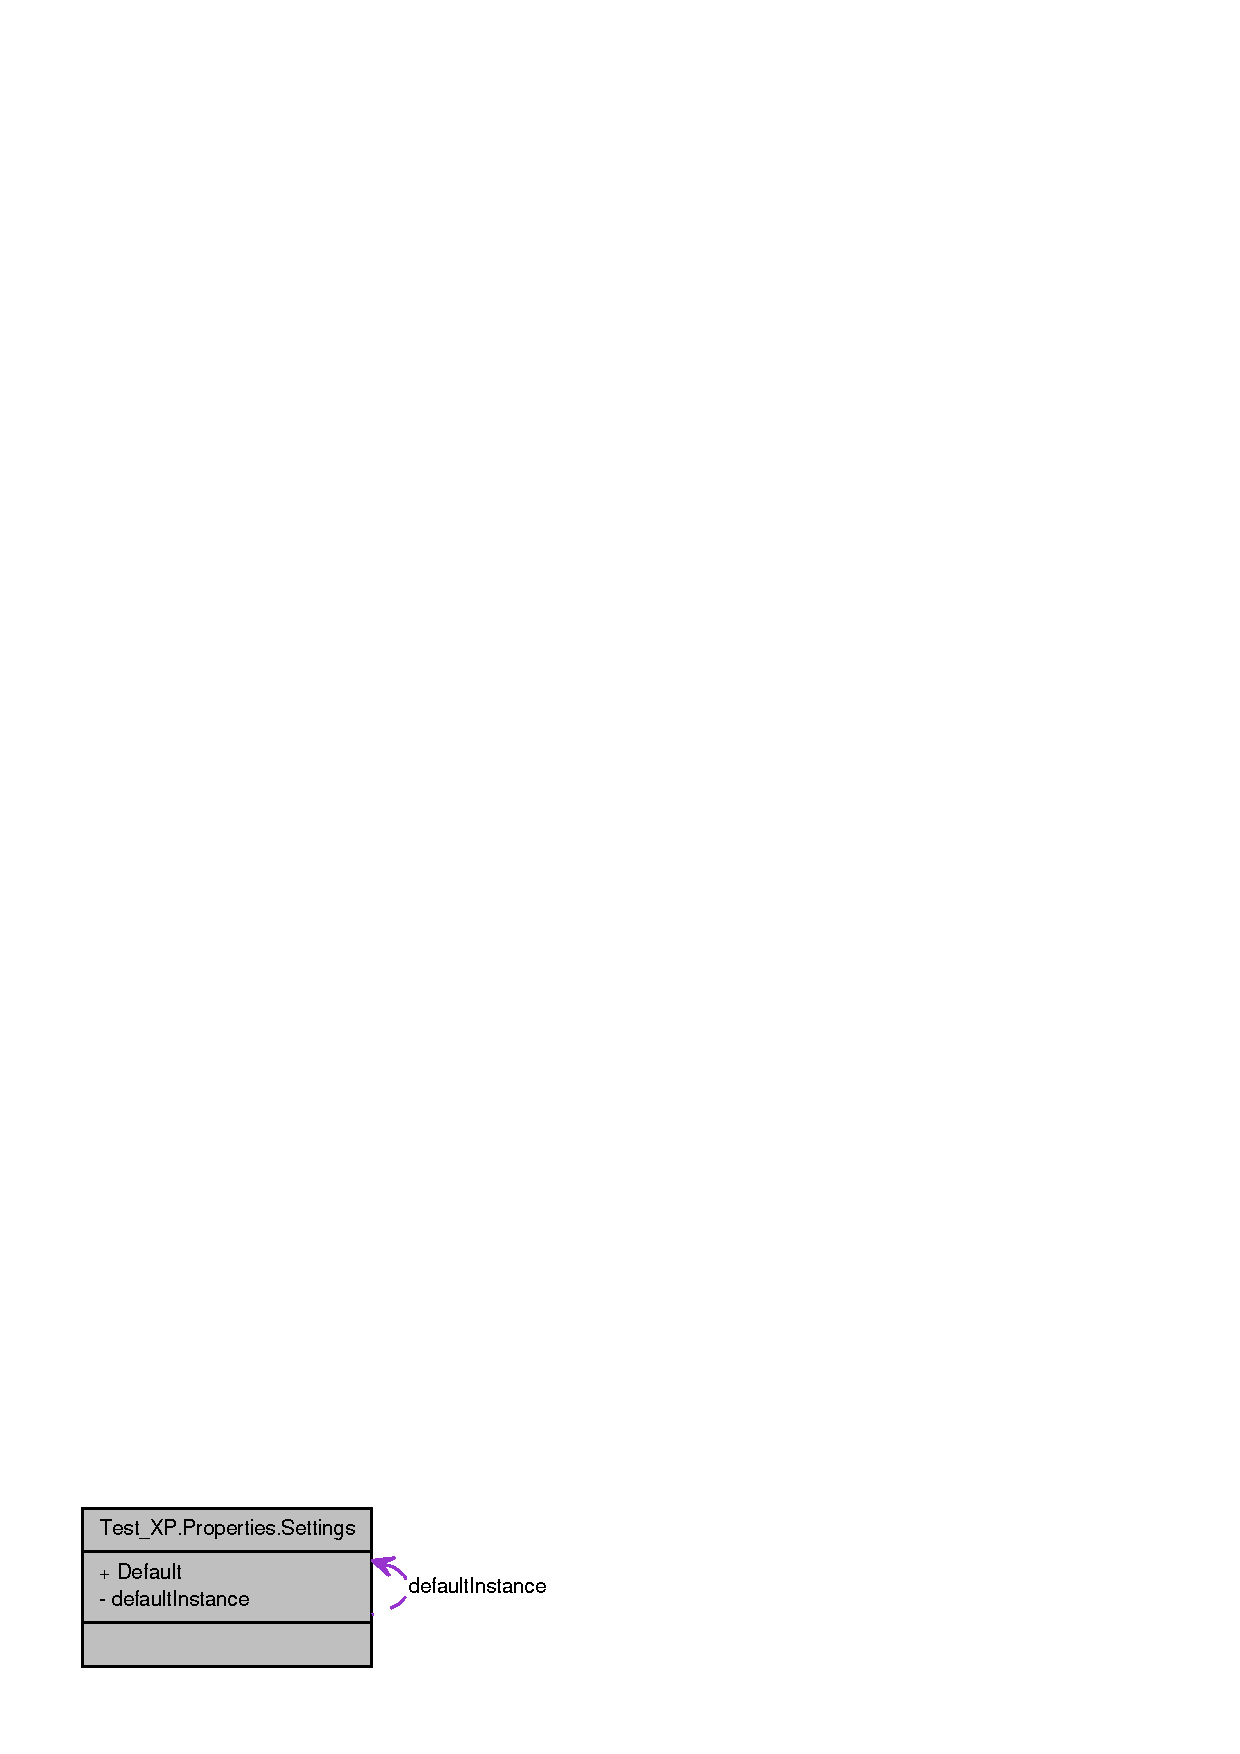
\includegraphics[width=266pt]{class_test___x_p_1_1_properties_1_1_settings__coll__graph}
\end{center}
\end{figure}
\subsection*{Propertys}
\begin{DoxyCompactItemize}
\item 
\hypertarget{class_test___x_p_1_1_properties_1_1_settings_a7a5870521771963698d03a258efb4c8e}{
static \hyperlink{class_test___x_p_1_1_properties_1_1_settings}{Settings} {\bfseries Default}\hspace{0.3cm}{\ttfamily  \mbox{[}get\mbox{]}}}
\label{class_test___x_p_1_1_properties_1_1_settings_a7a5870521771963698d03a258efb4c8e}

\end{DoxyCompactItemize}


Die Dokumentation für diese Klasse wurde erzeugt aufgrund der Datei:\begin{DoxyCompactItemize}
\item 
Test\_\-XP/Properties/Settings.Designer.cs\end{DoxyCompactItemize}

\hypertarget{class_test___console_1_1_properties_1_1_settings}{
\section{Test\_\-Console.Properties.Settings Klassenreferenz}
\label{class_test___console_1_1_properties_1_1_settings}\index{Test\_\-Console::Properties::Settings@{Test\_\-Console::Properties::Settings}}
}


Zusammengehörigkeiten von Test\_\-Console.Properties.Settings:\nopagebreak
\begin{figure}[H]
\begin{center}
\leavevmode
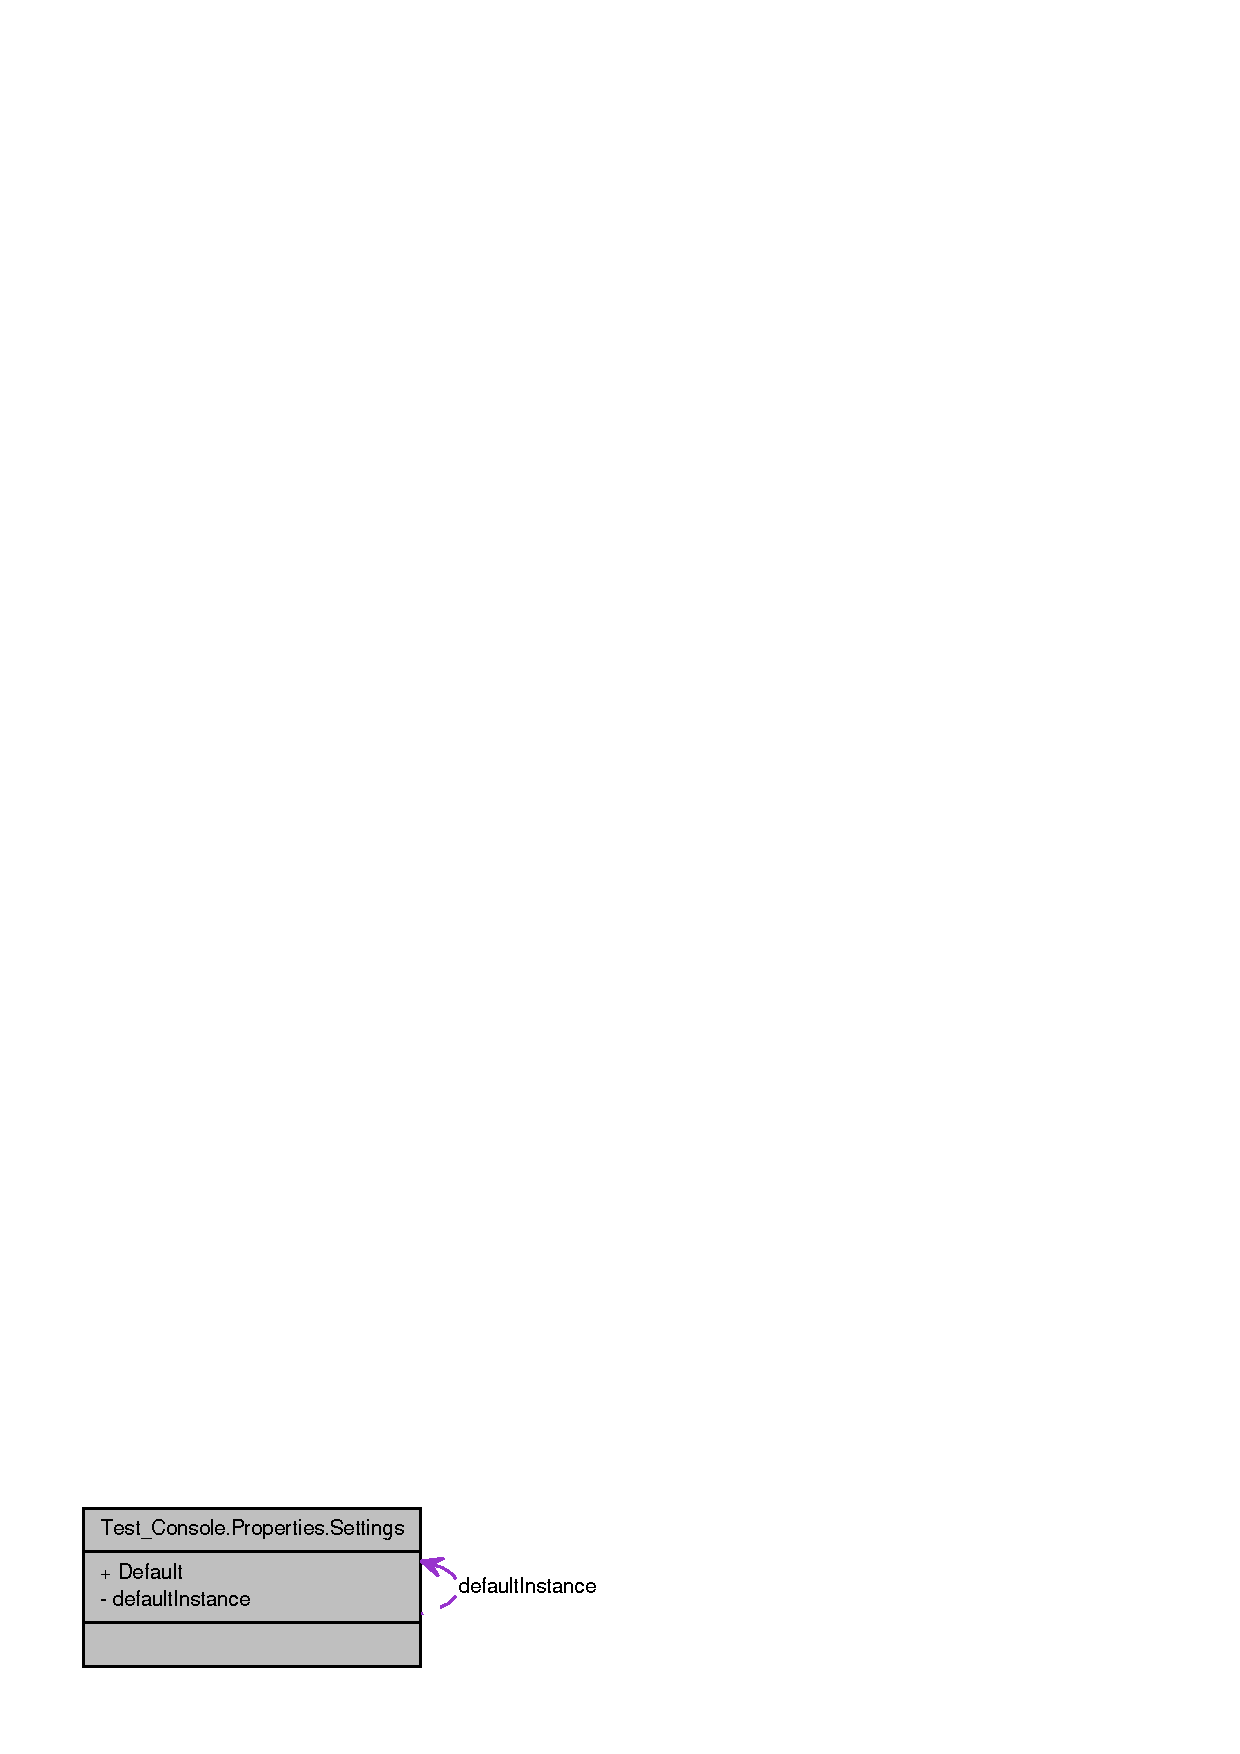
\includegraphics[width=290pt]{class_test___console_1_1_properties_1_1_settings__coll__graph}
\end{center}
\end{figure}
\subsection*{Propertys}
\begin{DoxyCompactItemize}
\item 
\hypertarget{class_test___console_1_1_properties_1_1_settings_a1c34923f97343187a84e157058e79b76}{
static \hyperlink{class_test___console_1_1_properties_1_1_settings}{Settings} {\bfseries Default}\hspace{0.3cm}{\ttfamily  \mbox{[}get\mbox{]}}}
\label{class_test___console_1_1_properties_1_1_settings_a1c34923f97343187a84e157058e79b76}

\end{DoxyCompactItemize}


Die Dokumentation für diese Klasse wurde erzeugt aufgrund der Datei:\begin{DoxyCompactItemize}
\item 
Test-\/Console/Properties/Settings.Designer.cs\end{DoxyCompactItemize}

\hypertarget{class_test___lamp_view_1_1_properties_1_1_settings}{
\section{Test\_\-LampView.Properties.Settings Klassenreferenz}
\label{class_test___lamp_view_1_1_properties_1_1_settings}\index{Test\_\-LampView::Properties::Settings@{Test\_\-LampView::Properties::Settings}}
}


Zusammengehörigkeiten von Test\_\-LampView.Properties.Settings:\nopagebreak
\begin{figure}[H]
\begin{center}
\leavevmode
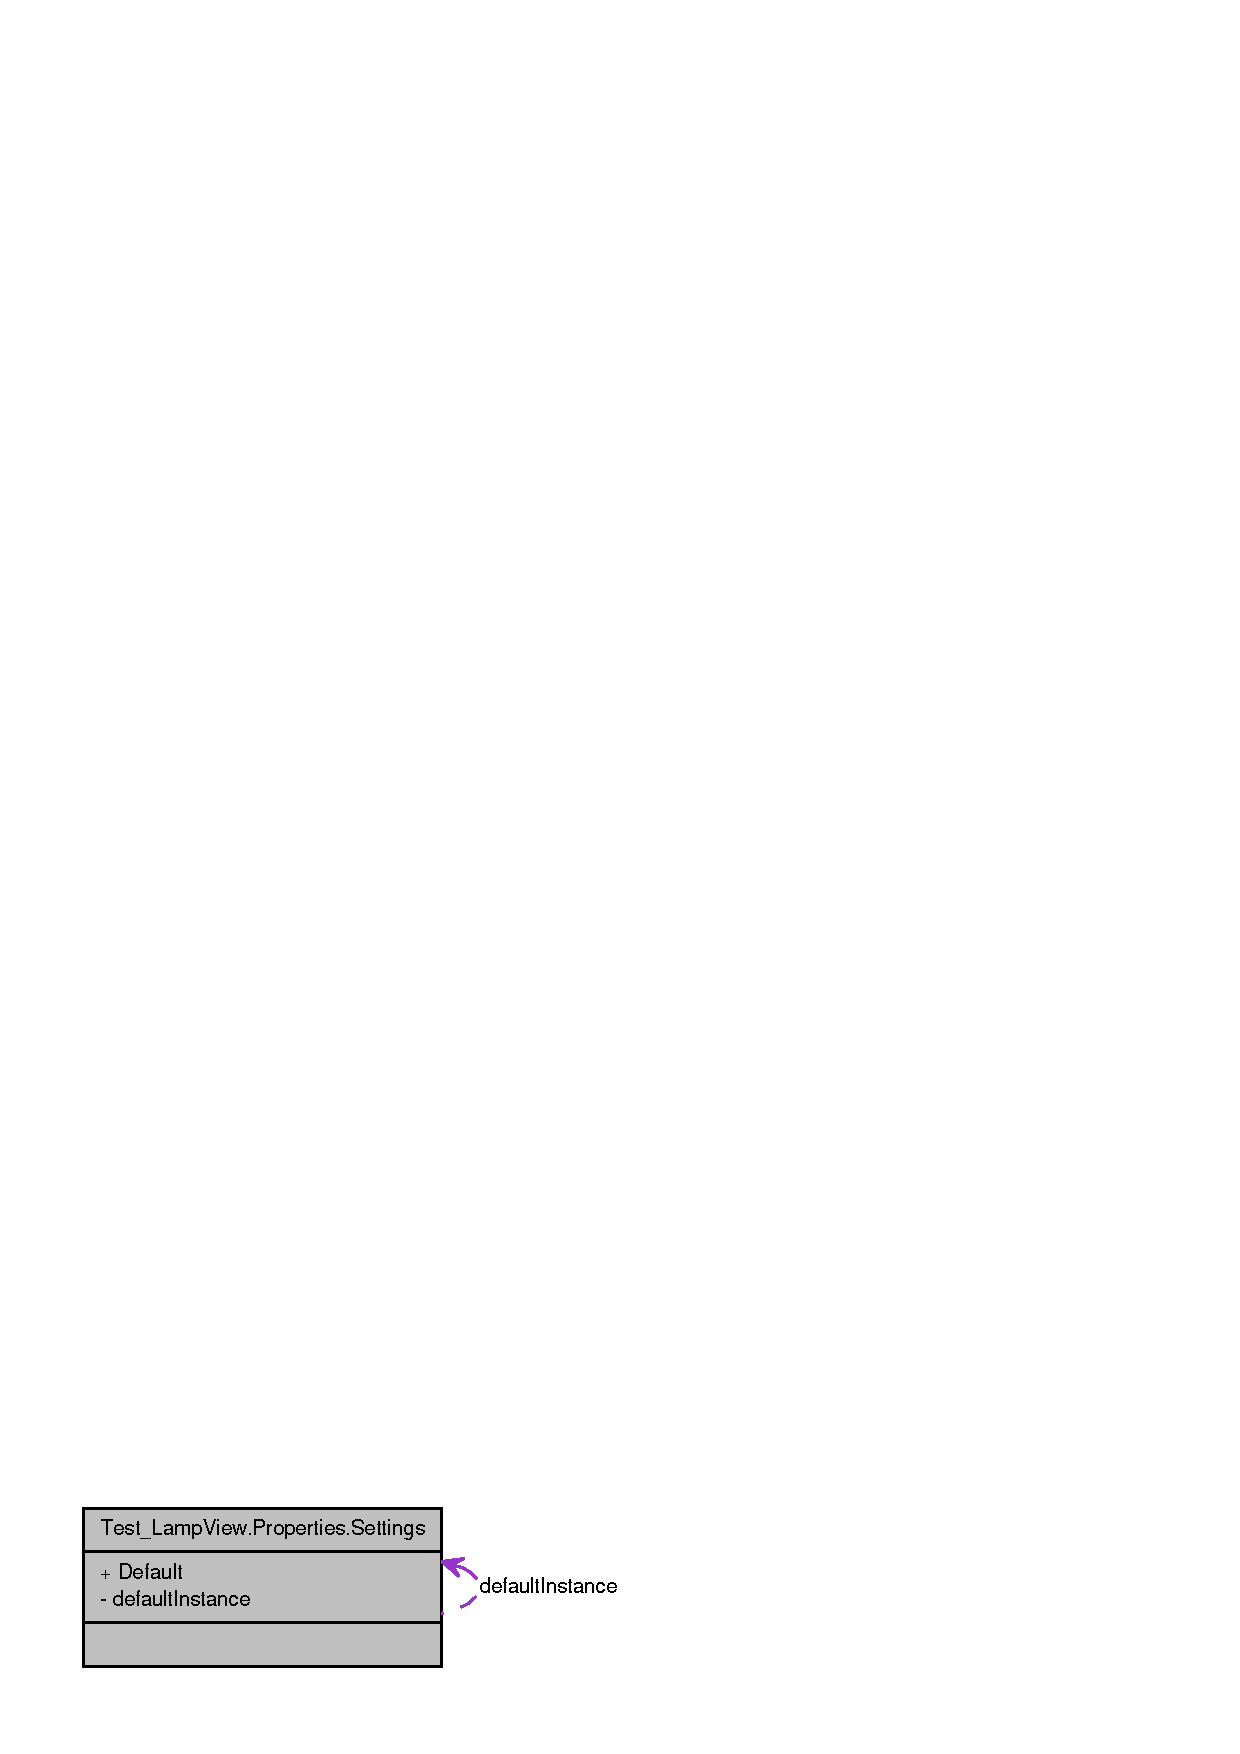
\includegraphics[width=300pt]{class_test___lamp_view_1_1_properties_1_1_settings__coll__graph}
\end{center}
\end{figure}
\subsection*{Propertys}
\begin{DoxyCompactItemize}
\item 
\hypertarget{class_test___lamp_view_1_1_properties_1_1_settings_a267d3826b179e5625ea4c88e093e5e73}{
static \hyperlink{class_test___lamp_view_1_1_properties_1_1_settings}{Settings} {\bfseries Default}\hspace{0.3cm}{\ttfamily  \mbox{[}get\mbox{]}}}
\label{class_test___lamp_view_1_1_properties_1_1_settings_a267d3826b179e5625ea4c88e093e5e73}

\end{DoxyCompactItemize}


Die Dokumentation für diese Klasse wurde erzeugt aufgrund der Datei:\begin{DoxyCompactItemize}
\item 
Test-\/LampView/Properties/Settings.Designer.cs\end{DoxyCompactItemize}

\hypertarget{class_test___drive___x_p_1_1_properties_1_1_settings}{
\section{Test\_\-Drive\_\-XP.Properties.Settings Klassenreferenz}
\label{class_test___drive___x_p_1_1_properties_1_1_settings}\index{Test\_\-Drive\_\-XP::Properties::Settings@{Test\_\-Drive\_\-XP::Properties::Settings}}
}


Zusammengehörigkeiten von Test\_\-Drive\_\-XP.Properties.Settings:\nopagebreak
\begin{figure}[H]
\begin{center}
\leavevmode
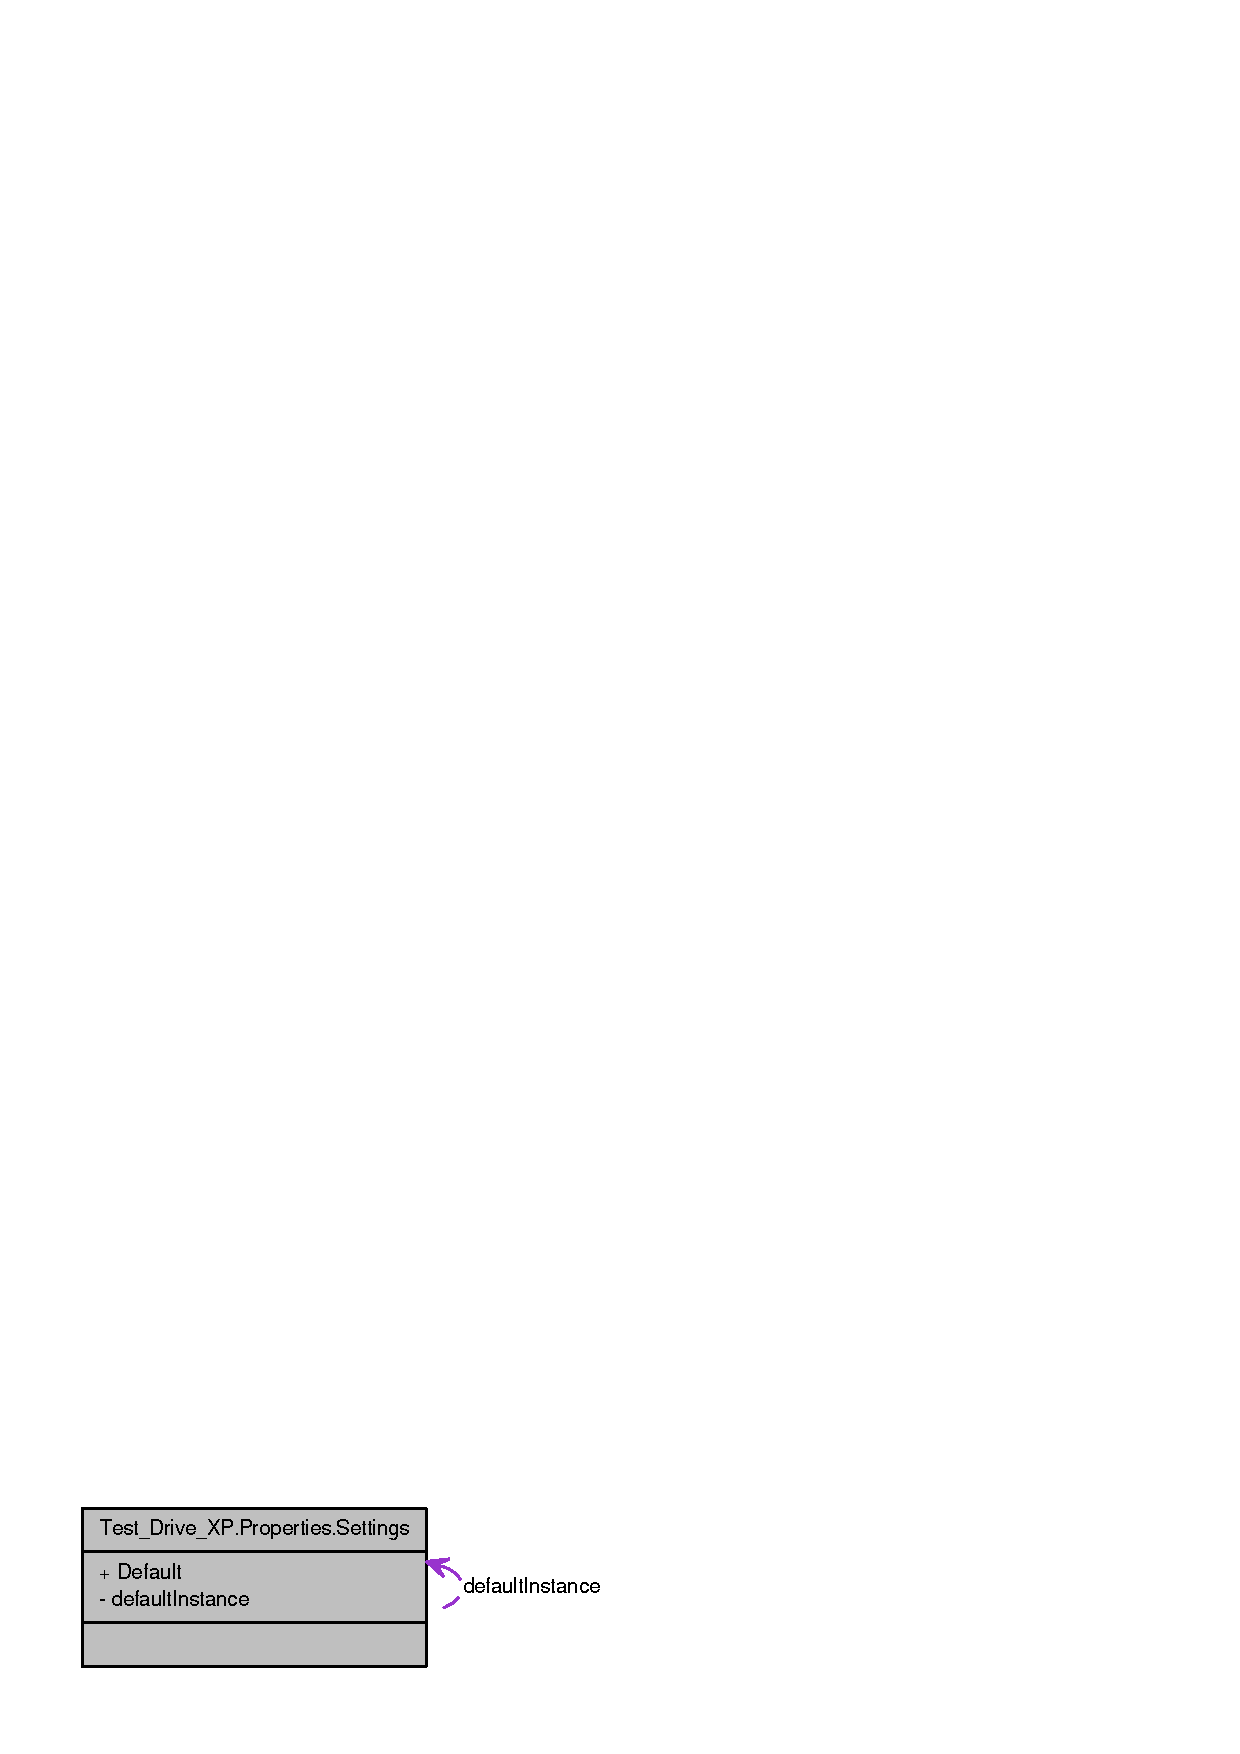
\includegraphics[width=292pt]{class_test___drive___x_p_1_1_properties_1_1_settings__coll__graph}
\end{center}
\end{figure}
\subsection*{Propertys}
\begin{DoxyCompactItemize}
\item 
\hypertarget{class_test___drive___x_p_1_1_properties_1_1_settings_ad479df3234d62ff6a42beeee68375587}{
static \hyperlink{class_test___drive___x_p_1_1_properties_1_1_settings}{Settings} {\bfseries Default}\hspace{0.3cm}{\ttfamily  \mbox{[}get\mbox{]}}}
\label{class_test___drive___x_p_1_1_properties_1_1_settings_ad479df3234d62ff6a42beeee68375587}

\end{DoxyCompactItemize}


Die Dokumentation für diese Klasse wurde erzeugt aufgrund der Datei:\begin{DoxyCompactItemize}
\item 
Test\_\-Drive\_\-XP/Properties/Settings.Designer.cs\end{DoxyCompactItemize}

\hypertarget{class_test___motor___x_p_1_1_properties_1_1_settings}{
\section{Test\_\-Motor\_\-XP.Properties.Settings Klassenreferenz}
\label{class_test___motor___x_p_1_1_properties_1_1_settings}\index{Test\_\-Motor\_\-XP::Properties::Settings@{Test\_\-Motor\_\-XP::Properties::Settings}}
}


Zusammengehörigkeiten von Test\_\-Motor\_\-XP.Properties.Settings:\nopagebreak
\begin{figure}[H]
\begin{center}
\leavevmode
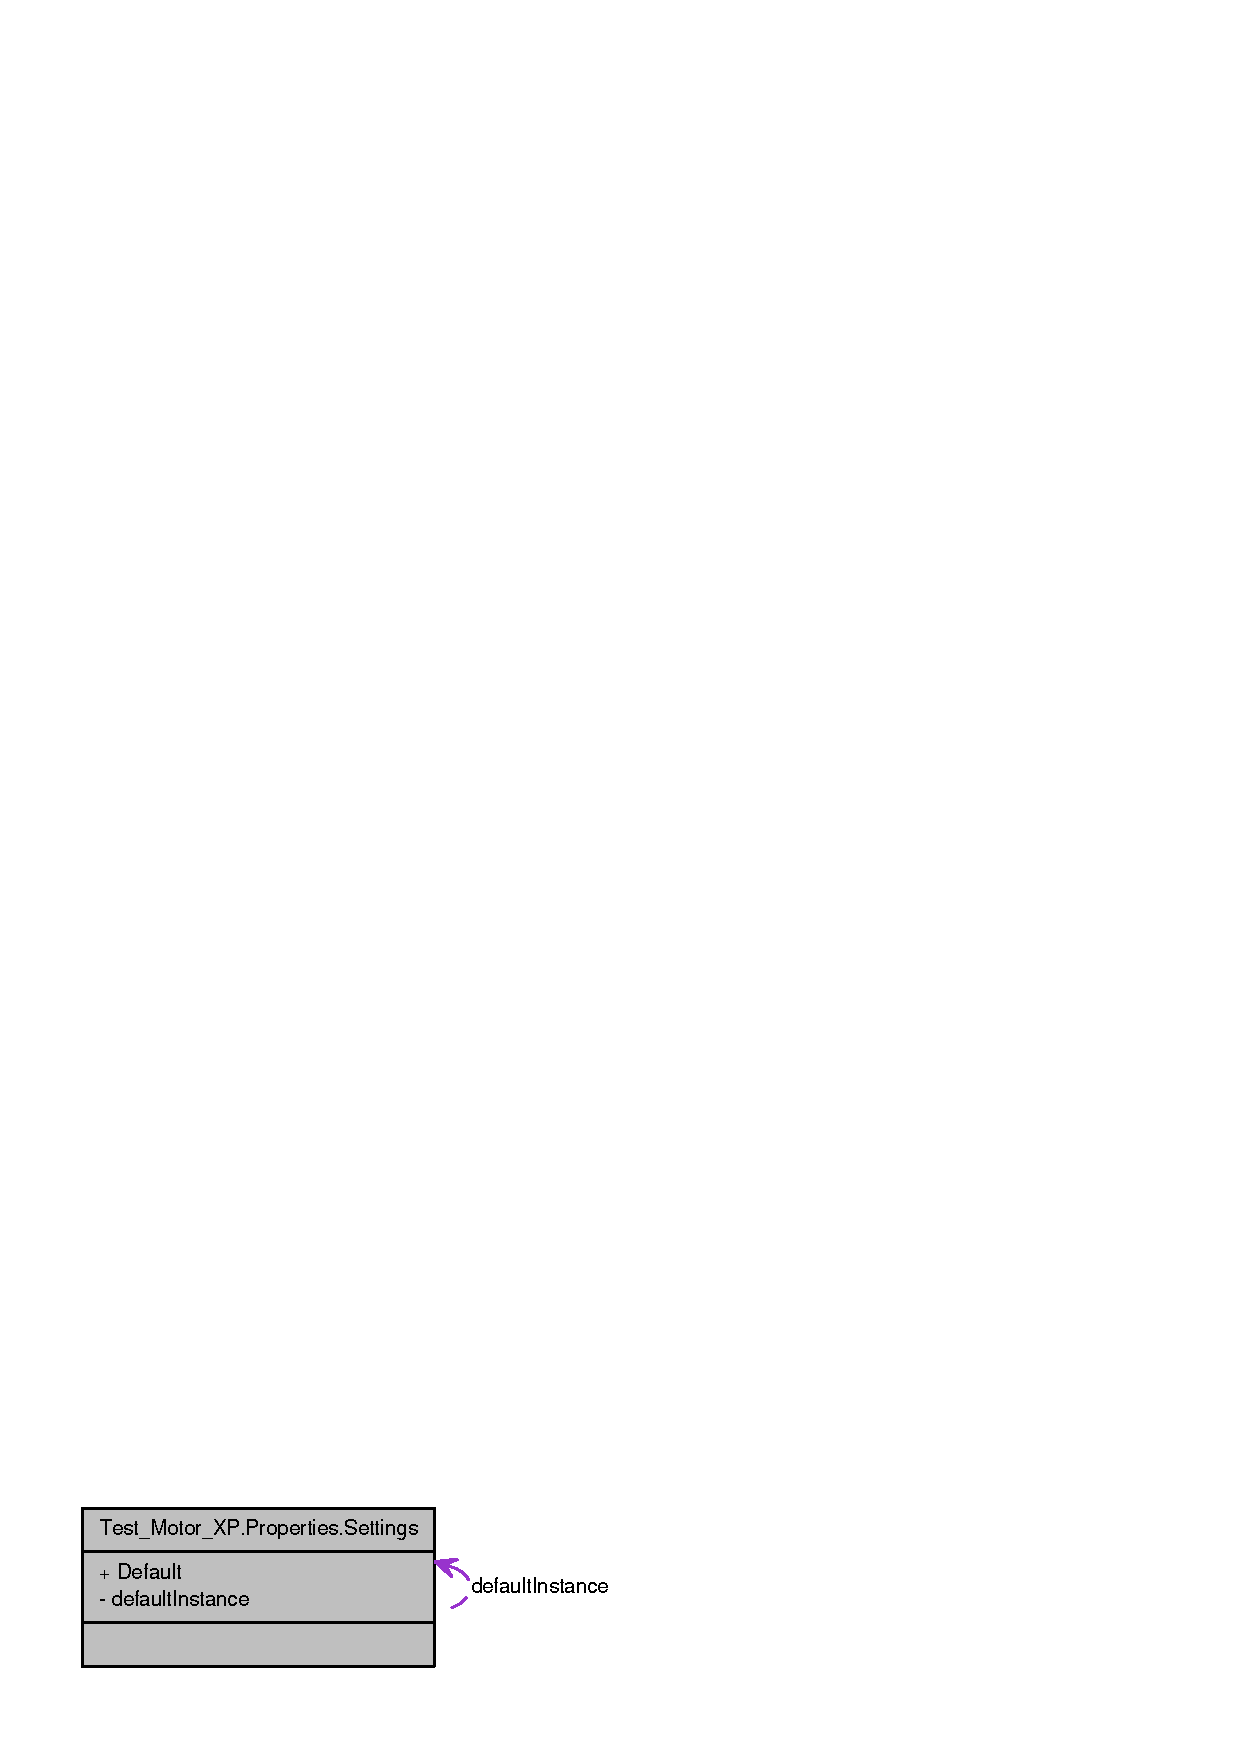
\includegraphics[width=296pt]{class_test___motor___x_p_1_1_properties_1_1_settings__coll__graph}
\end{center}
\end{figure}
\subsection*{Propertys}
\begin{DoxyCompactItemize}
\item 
\hypertarget{class_test___motor___x_p_1_1_properties_1_1_settings_a73814e6a8d37076545f0172973c8ff33}{
static \hyperlink{class_test___motor___x_p_1_1_properties_1_1_settings}{Settings} {\bfseries Default}\hspace{0.3cm}{\ttfamily  \mbox{[}get\mbox{]}}}
\label{class_test___motor___x_p_1_1_properties_1_1_settings_a73814e6a8d37076545f0172973c8ff33}

\end{DoxyCompactItemize}


Die Dokumentation für diese Klasse wurde erzeugt aufgrund der Datei:\begin{DoxyCompactItemize}
\item 
Test\_\-Motor\_\-XP/Properties/Settings.Designer.cs\end{DoxyCompactItemize}

\hypertarget{class_robot_view_1_1_switch_event_arg}{
\section{RobotView.SwitchEventArg Klassenreferenz}
\label{class_robot_view_1_1_switch_event_arg}\index{RobotView::SwitchEventArg@{RobotView::SwitchEventArg}}
}


Klasse implementiert einen EventArg, der einen boolean State des Switches repräsentiert.  


\subsection*{Öffentliche Methoden}
\begin{DoxyCompactItemize}
\item 
\hyperlink{class_robot_view_1_1_switch_event_arg_a2112bc72be277bbfc8190aae7f65274e}{SwitchEventArg} (bool state)
\begin{DoxyCompactList}\small\item\em Constructor um dem Event einen boolean State mitzugeben. \item\end{DoxyCompactList}\end{DoxyCompactItemize}
\subsection*{Propertys}
\begin{DoxyCompactItemize}
\item 
bool \hyperlink{class_robot_view_1_1_switch_event_arg_a6c1441d3012ab67cbff2ffe52f3ad625}{State}\hspace{0.3cm}{\ttfamily  \mbox{[}get\mbox{]}}
\begin{DoxyCompactList}\small\item\em Property um den State abzufragen. \item\end{DoxyCompactList}\end{DoxyCompactItemize}


\subsection{Ausführliche Beschreibung}
Klasse implementiert einen EventArg, der einen boolean State des Switches repräsentiert. 

\subsection{Beschreibung der Konstruktoren und Destruktoren}
\hypertarget{class_robot_view_1_1_switch_event_arg_a2112bc72be277bbfc8190aae7f65274e}{
\index{RobotView::SwitchEventArg@{RobotView::SwitchEventArg}!SwitchEventArg@{SwitchEventArg}}
\index{SwitchEventArg@{SwitchEventArg}!RobotView::SwitchEventArg@{RobotView::SwitchEventArg}}
\subsubsection[{SwitchEventArg}]{\setlength{\rightskip}{0pt plus 5cm}RobotView.SwitchEventArg.SwitchEventArg (bool {\em state})}}
\label{class_robot_view_1_1_switch_event_arg_a2112bc72be277bbfc8190aae7f65274e}


Constructor um dem Event einen boolean State mitzugeben. 


\begin{DoxyParams}{Parameter}
\item[{\em state}]\end{DoxyParams}


\subsection{Dokumentation der Propertys}
\hypertarget{class_robot_view_1_1_switch_event_arg_a6c1441d3012ab67cbff2ffe52f3ad625}{
\index{RobotView::SwitchEventArg@{RobotView::SwitchEventArg}!State@{State}}
\index{State@{State}!RobotView::SwitchEventArg@{RobotView::SwitchEventArg}}
\subsubsection[{State}]{\setlength{\rightskip}{0pt plus 5cm}bool RobotView.SwitchEventArg.State\hspace{0.3cm}{\ttfamily  \mbox{[}get\mbox{]}}}}
\label{class_robot_view_1_1_switch_event_arg_a6c1441d3012ab67cbff2ffe52f3ad625}


Property um den State abzufragen. 

\begin{DoxyReturn}{Rückgabe}
true or false 
\end{DoxyReturn}


Die Dokumentation für diese Klasse wurde erzeugt aufgrund der Datei:\begin{DoxyCompactItemize}
\item 
SwitchView.cs\end{DoxyCompactItemize}

\hypertarget{class_robot_view_1_1_switch_view}{
\section{RobotView.SwitchView Klassenreferenz}
\label{class_robot_view_1_1_switch_view}\index{RobotView::SwitchView@{RobotView::SwitchView}}
}


Klasse die einen einzelnen Switch darstellt. Wird Verwendet um einen Switch des HSLU Roboters darzustellen.  


\subsection*{Öffentliche Methoden}
\begin{DoxyCompactItemize}
\item 
\hyperlink{class_robot_view_1_1_switch_view_adf984c63fc036efa55ca459e25a5cefd}{SwitchView} ()
\begin{DoxyCompactList}\small\item\em Standardkonstruktor. \item\end{DoxyCompactList}\end{DoxyCompactItemize}
\subsection*{Propertys}
\begin{DoxyCompactItemize}
\item 
bool \hyperlink{class_robot_view_1_1_switch_view_a78d6236230e163636d827c42cccdfbd9}{State}\hspace{0.3cm}{\ttfamily  \mbox{[}get, set\mbox{]}}
\begin{DoxyCompactList}\small\item\em Setzen oder abfragen des aktuellen Switch Status. \item\end{DoxyCompactList}\end{DoxyCompactItemize}
\subsection*{Ereignisse}
\begin{DoxyCompactItemize}
\item 
System.EventHandler \hyperlink{class_robot_view_1_1_switch_view_a2254d22e9d9d1fd1fae8208f52d689d0}{SwitchChanged}
\begin{DoxyCompactList}\small\item\em Hier kann man einen EventHandler registrieren. \item\end{DoxyCompactList}\end{DoxyCompactItemize}


\subsection{Ausführliche Beschreibung}
Klasse die einen einzelnen Switch darstellt. Wird Verwendet um einen Switch des HSLU Roboters darzustellen. {\ttfamily  \hyperlink{class_robot_view_1_1_switch_view}{SwitchView} switchView = new \hyperlink{class_robot_view_1_1_switch_view_adf984c63fc036efa55ca459e25a5cefd}{SwitchView()}; switchView.Location = new System.Drawing.Point(22 + 95, 2); switchView.SwitchChanged += SwitchChanged\_\-Handler; } 

\subsection{Beschreibung der Konstruktoren und Destruktoren}
\hypertarget{class_robot_view_1_1_switch_view_adf984c63fc036efa55ca459e25a5cefd}{
\index{RobotView::SwitchView@{RobotView::SwitchView}!SwitchView@{SwitchView}}
\index{SwitchView@{SwitchView}!RobotView::SwitchView@{RobotView::SwitchView}}
\subsubsection[{SwitchView}]{\setlength{\rightskip}{0pt plus 5cm}RobotView.SwitchView.SwitchView ()}}
\label{class_robot_view_1_1_switch_view_adf984c63fc036efa55ca459e25a5cefd}


Standardkonstruktor. 



\subsection{Dokumentation der Propertys}
\hypertarget{class_robot_view_1_1_switch_view_a78d6236230e163636d827c42cccdfbd9}{
\index{RobotView::SwitchView@{RobotView::SwitchView}!State@{State}}
\index{State@{State}!RobotView::SwitchView@{RobotView::SwitchView}}
\subsubsection[{State}]{\setlength{\rightskip}{0pt plus 5cm}bool RobotView.SwitchView.State\hspace{0.3cm}{\ttfamily  \mbox{[}get, set\mbox{]}}}}
\label{class_robot_view_1_1_switch_view_a78d6236230e163636d827c42cccdfbd9}


Setzen oder abfragen des aktuellen Switch Status. 



\subsection{Ereignisdokumentation}
\hypertarget{class_robot_view_1_1_switch_view_a2254d22e9d9d1fd1fae8208f52d689d0}{
\index{RobotView::SwitchView@{RobotView::SwitchView}!SwitchChanged@{SwitchChanged}}
\index{SwitchChanged@{SwitchChanged}!RobotView::SwitchView@{RobotView::SwitchView}}
\subsubsection[{SwitchChanged}]{\setlength{\rightskip}{0pt plus 5cm}System.EventHandler RobotView.SwitchView.SwitchChanged}}
\label{class_robot_view_1_1_switch_view_a2254d22e9d9d1fd1fae8208f52d689d0}


Hier kann man einen EventHandler registrieren. 



Die Dokumentation für diese Klasse wurde erzeugt aufgrund der Datei:\begin{DoxyCompactItemize}
\item 
SwitchView.cs\end{DoxyCompactItemize}

\hypertarget{class_test___c_e_1_1_test___c_e___form}{
\section{Test\_\-CE.Test\_\-CE\_\-Form Klassenreferenz}
\label{class_test___c_e_1_1_test___c_e___form}\index{Test\_\-CE::Test\_\-CE\_\-Form@{Test\_\-CE::Test\_\-CE\_\-Form}}
}


Zusammengehörigkeiten von Test\_\-CE.Test\_\-CE\_\-Form:\nopagebreak
\begin{figure}[H]
\begin{center}
\leavevmode
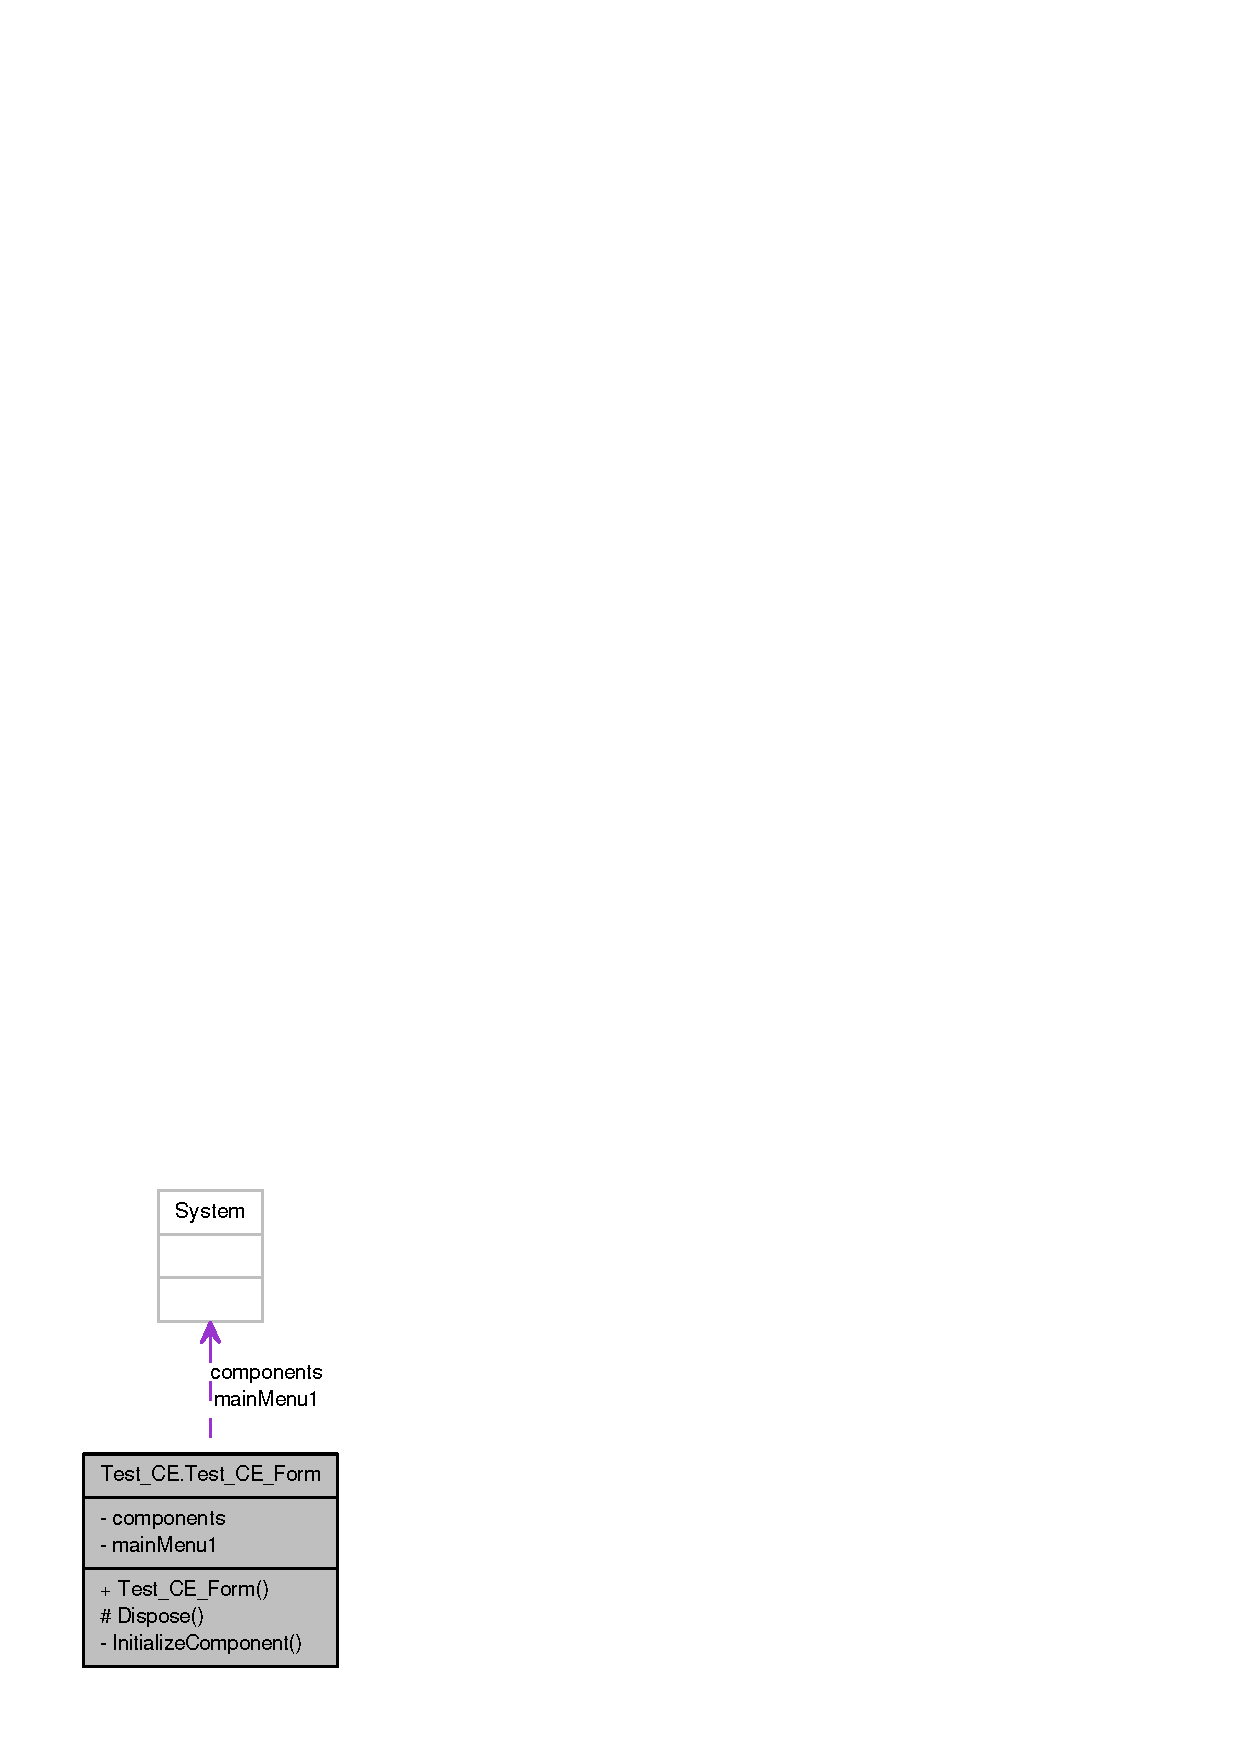
\includegraphics[width=166pt]{class_test___c_e_1_1_test___c_e___form__coll__graph}
\end{center}
\end{figure}
\subsection*{Geschützte Methoden}
\begin{DoxyCompactItemize}
\item 
override void \hyperlink{class_test___c_e_1_1_test___c_e___form_aae767bb52af6d4e5a187f8810fea9d2f}{Dispose} (bool disposing)
\begin{DoxyCompactList}\small\item\em Verwendete Ressourcen bereinigen. \item\end{DoxyCompactList}\end{DoxyCompactItemize}


\subsection{Dokumentation der Elementfunktionen}
\hypertarget{class_test___c_e_1_1_test___c_e___form_aae767bb52af6d4e5a187f8810fea9d2f}{
\index{Test\_\-CE::Test\_\-CE\_\-Form@{Test\_\-CE::Test\_\-CE\_\-Form}!Dispose@{Dispose}}
\index{Dispose@{Dispose}!Test_CE::Test_CE_Form@{Test\_\-CE::Test\_\-CE\_\-Form}}
\subsubsection[{Dispose}]{\setlength{\rightskip}{0pt plus 5cm}override void Test\_\-CE.Test\_\-CE\_\-Form.Dispose (bool {\em disposing})\hspace{0.3cm}{\ttfamily  \mbox{[}protected\mbox{]}}}}
\label{class_test___c_e_1_1_test___c_e___form_aae767bb52af6d4e5a187f8810fea9d2f}


Verwendete Ressourcen bereinigen. 


\begin{DoxyParams}{Parameter}
\item[{\em disposing}]True, wenn verwaltete Ressourcen gelöscht werden sollen; andernfalls False.\end{DoxyParams}


Die Dokumentation für diese Klasse wurde erzeugt aufgrund der Dateien:\begin{DoxyCompactItemize}
\item 
Test\_\-CE\_\-Form.cs\item 
Test\_\-CE\_\-Form.Designer.cs\end{DoxyCompactItemize}

\hypertarget{class_robot_ctrl_1_1_track}{
\section{RobotCtrl.Track Klassenreferenz}
\label{class_robot_ctrl_1_1_track}\index{RobotCtrl::Track@{RobotCtrl::Track}}
}


Klassendiagramm für RobotCtrl.Track:\nopagebreak
\begin{figure}[H]
\begin{center}
\leavevmode
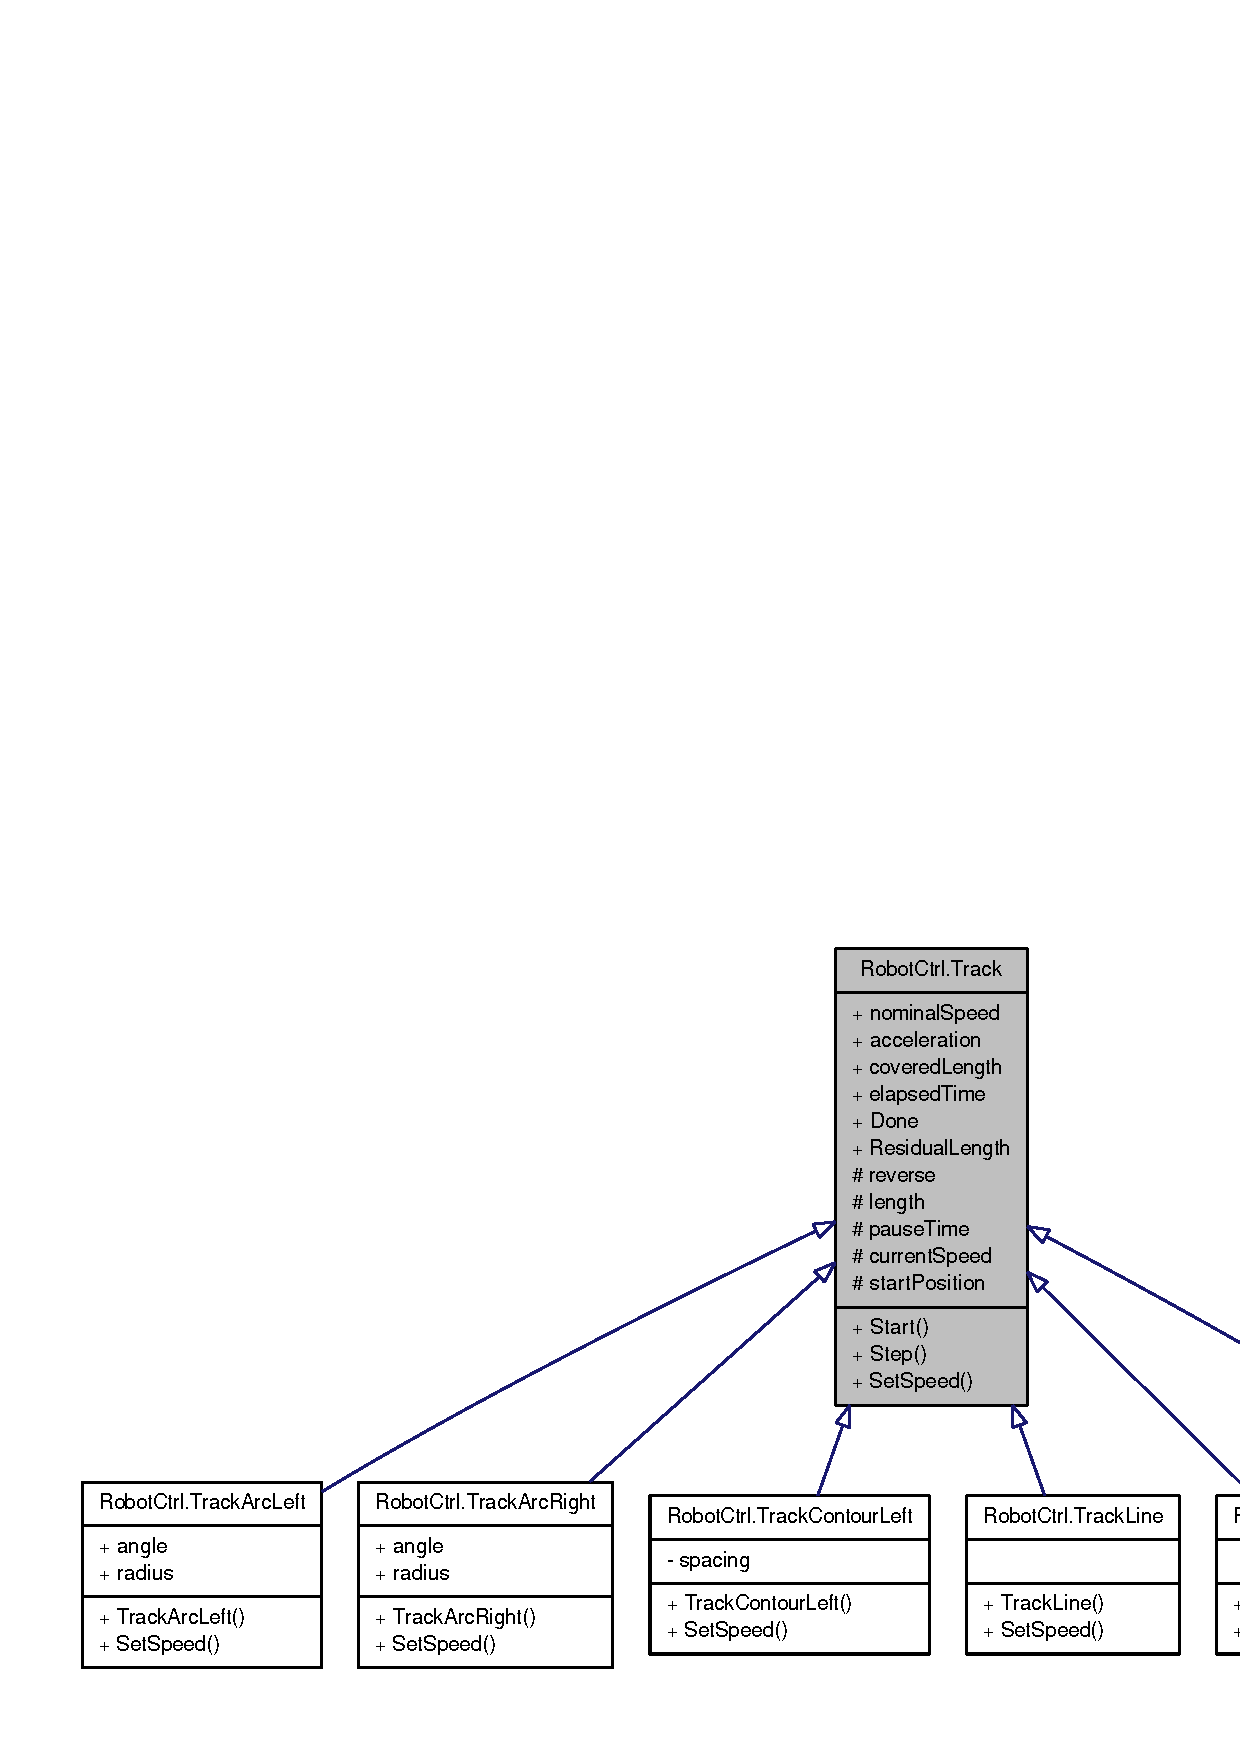
\includegraphics[width=400pt]{class_robot_ctrl_1_1_track__inherit__graph}
\end{center}
\end{figure}


Zusammengehörigkeiten von RobotCtrl.Track:\nopagebreak
\begin{figure}[H]
\begin{center}
\leavevmode
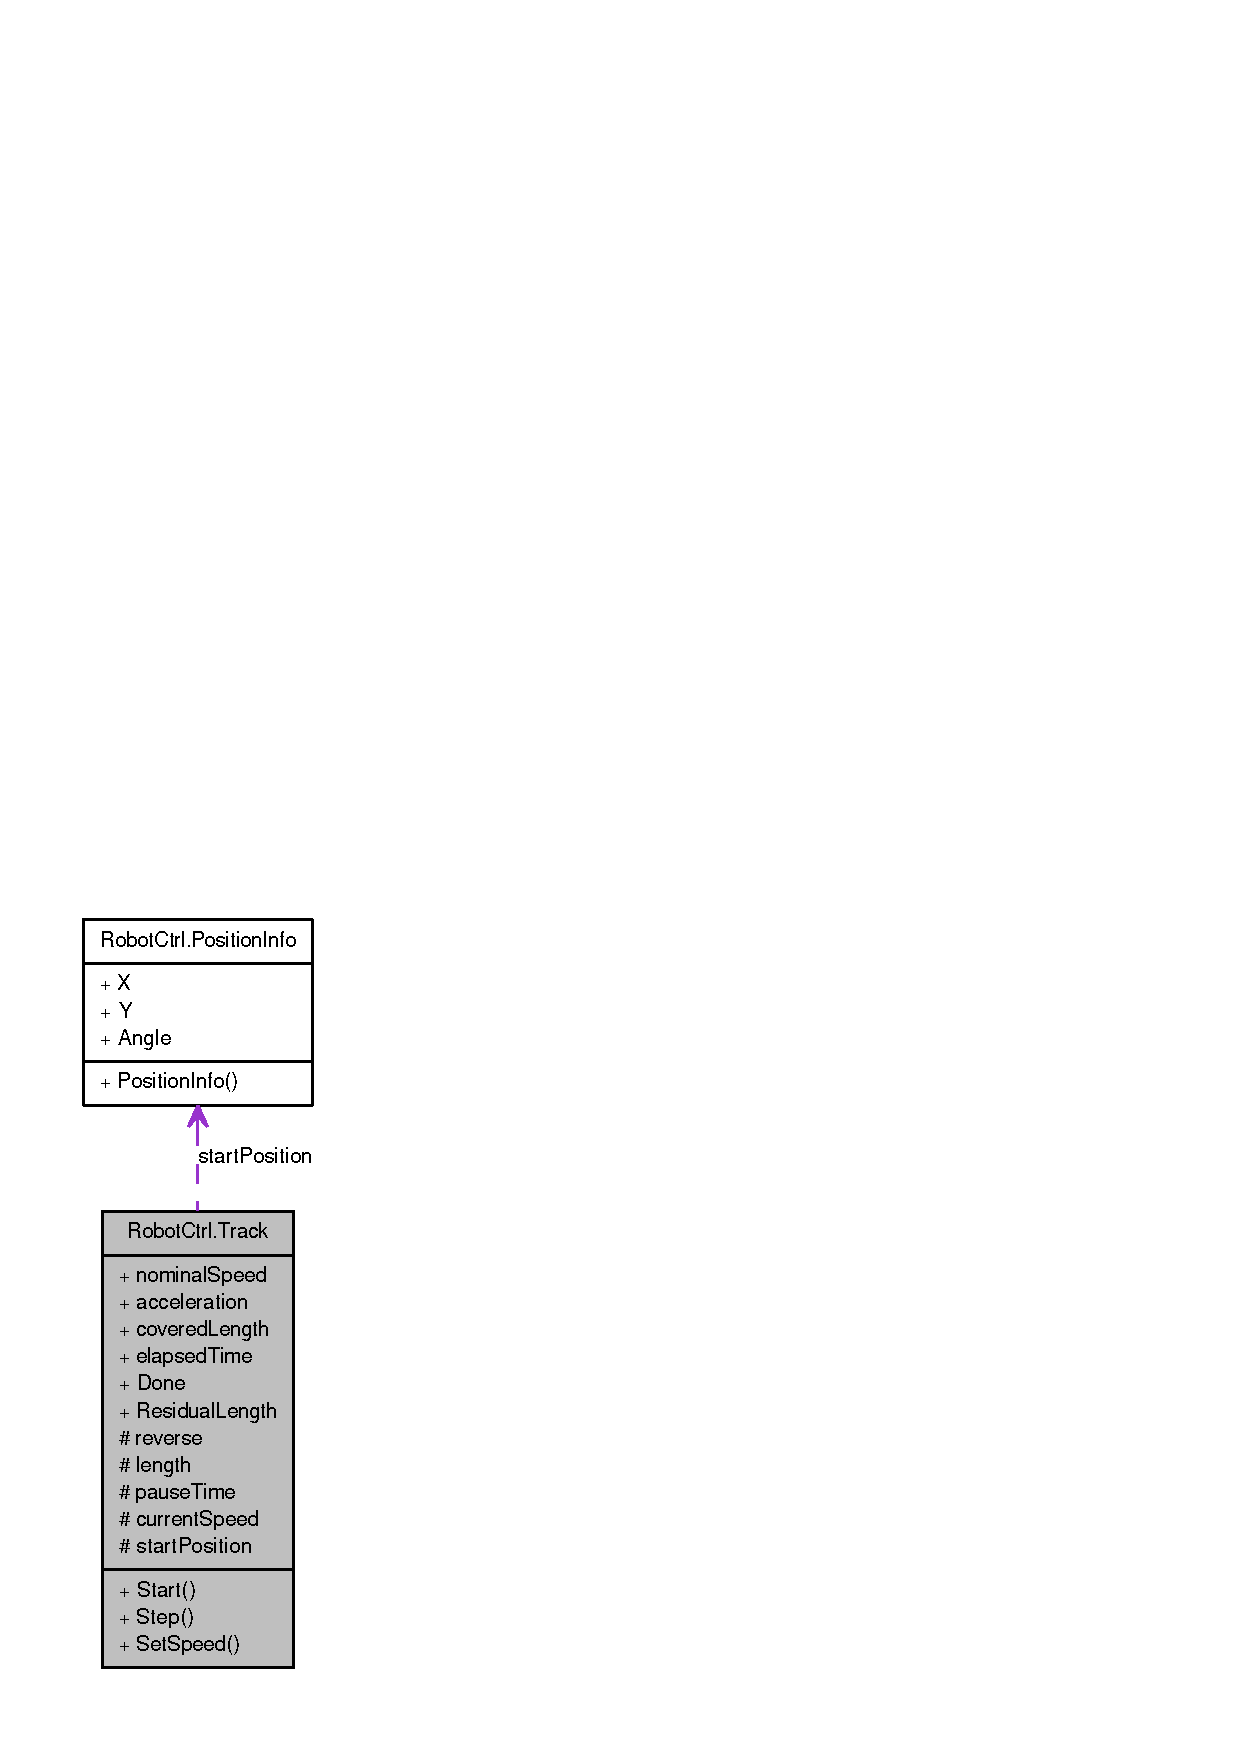
\includegraphics[height=400pt]{class_robot_ctrl_1_1_track__coll__graph}
\end{center}
\end{figure}
\subsection*{Öffentliche Methoden}
\begin{DoxyCompactItemize}
\item 
\hypertarget{class_robot_ctrl_1_1_track_a91c0b372e1c332ae1aa18368df116633}{
virtual void {\bfseries Start} (\hyperlink{struct_robot_ctrl_1_1_position_info}{PositionInfo} startPosition)}
\label{class_robot_ctrl_1_1_track_a91c0b372e1c332ae1aa18368df116633}

\item 
\hypertarget{class_robot_ctrl_1_1_track_a82386b9a49faa6a31d9706f39238f21b}{
virtual void {\bfseries Step} (double timeInterval)}
\label{class_robot_ctrl_1_1_track_a82386b9a49faa6a31d9706f39238f21b}

\item 
\hypertarget{class_robot_ctrl_1_1_track_a9abc3ccf4bf1d9db8d461f2cb4b4b0d3}{
virtual void {\bfseries SetSpeed} (double newSpeed, \hyperlink{class_robot_ctrl_1_1_motor_ctrl}{MotorCtrl} left, \hyperlink{class_robot_ctrl_1_1_motor_ctrl}{MotorCtrl} right)}
\label{class_robot_ctrl_1_1_track_a9abc3ccf4bf1d9db8d461f2cb4b4b0d3}

\end{DoxyCompactItemize}
\subsection*{Öffentliche Attribute}
\begin{DoxyCompactItemize}
\item 
\hypertarget{class_robot_ctrl_1_1_track_a7d996b14578c6059e6868e2210e1d582}{
double {\bfseries nominalSpeed}}
\label{class_robot_ctrl_1_1_track_a7d996b14578c6059e6868e2210e1d582}

\item 
\hypertarget{class_robot_ctrl_1_1_track_abf40e28208ac9861b7f75042fcb68d20}{
double {\bfseries acceleration}}
\label{class_robot_ctrl_1_1_track_abf40e28208ac9861b7f75042fcb68d20}

\item 
\hypertarget{class_robot_ctrl_1_1_track_a590aa4c79e81feedcc5116a874d88e4d}{
double {\bfseries coveredLength}}
\label{class_robot_ctrl_1_1_track_a590aa4c79e81feedcc5116a874d88e4d}

\item 
\hypertarget{class_robot_ctrl_1_1_track_a17436774d1af50ddffc88f505728f713}{
double {\bfseries elapsedTime}}
\label{class_robot_ctrl_1_1_track_a17436774d1af50ddffc88f505728f713}

\end{DoxyCompactItemize}
\subsection*{Geschützte Attribute}
\begin{DoxyCompactItemize}
\item 
\hypertarget{class_robot_ctrl_1_1_track_a98f9e9a8f087b8c7770d8f8320d821c5}{
bool {\bfseries reverse} = false}
\label{class_robot_ctrl_1_1_track_a98f9e9a8f087b8c7770d8f8320d821c5}

\item 
\hypertarget{class_robot_ctrl_1_1_track_ad4fd8df6c4813180fe764d327a9a9af8}{
double {\bfseries length} = 0}
\label{class_robot_ctrl_1_1_track_ad4fd8df6c4813180fe764d327a9a9af8}

\item 
\hypertarget{class_robot_ctrl_1_1_track_a98771bf28c921adf67e6df981dcf8e2a}{
double {\bfseries pauseTime} = 0}
\label{class_robot_ctrl_1_1_track_a98771bf28c921adf67e6df981dcf8e2a}

\item 
\hypertarget{class_robot_ctrl_1_1_track_ac8722c422d19d4b18430b106275bc9f9}{
double {\bfseries currentSpeed} = 0}
\label{class_robot_ctrl_1_1_track_ac8722c422d19d4b18430b106275bc9f9}

\item 
\hypertarget{class_robot_ctrl_1_1_track_a731b5abc7baa77c51b72c5dea7cbfba8}{
\hyperlink{struct_robot_ctrl_1_1_position_info}{PositionInfo} {\bfseries startPosition}}
\label{class_robot_ctrl_1_1_track_a731b5abc7baa77c51b72c5dea7cbfba8}

\end{DoxyCompactItemize}
\subsection*{Propertys}
\begin{DoxyCompactItemize}
\item 
\hypertarget{class_robot_ctrl_1_1_track_ad1c4864f7171475914ef5c0111a0d901}{
virtual bool {\bfseries Done}\hspace{0.3cm}{\ttfamily  \mbox{[}get\mbox{]}}}
\label{class_robot_ctrl_1_1_track_ad1c4864f7171475914ef5c0111a0d901}

\item 
\hypertarget{class_robot_ctrl_1_1_track_a4f01da358c21733d43ac272d3fb549cc}{
virtual double {\bfseries ResidualLength}\hspace{0.3cm}{\ttfamily  \mbox{[}get\mbox{]}}}
\label{class_robot_ctrl_1_1_track_a4f01da358c21733d43ac272d3fb549cc}

\end{DoxyCompactItemize}


Die Dokumentation für diese Klasse wurde erzeugt aufgrund der Datei:\begin{DoxyCompactItemize}
\item 
Track.cs\end{DoxyCompactItemize}

\hypertarget{class_robot_ctrl_1_1_track_arc_left}{
\section{RobotCtrl.TrackArcLeft Klassenreferenz}
\label{class_robot_ctrl_1_1_track_arc_left}\index{RobotCtrl::TrackArcLeft@{RobotCtrl::TrackArcLeft}}
}


\hyperlink{class_robot_ctrl_1_1_track_arc_left}{TrackArcLeft} wird verwendet um einen Bogen nach links zu fahren.  




Klassendiagramm für RobotCtrl.TrackArcLeft:\nopagebreak
\begin{figure}[H]
\begin{center}
\leavevmode
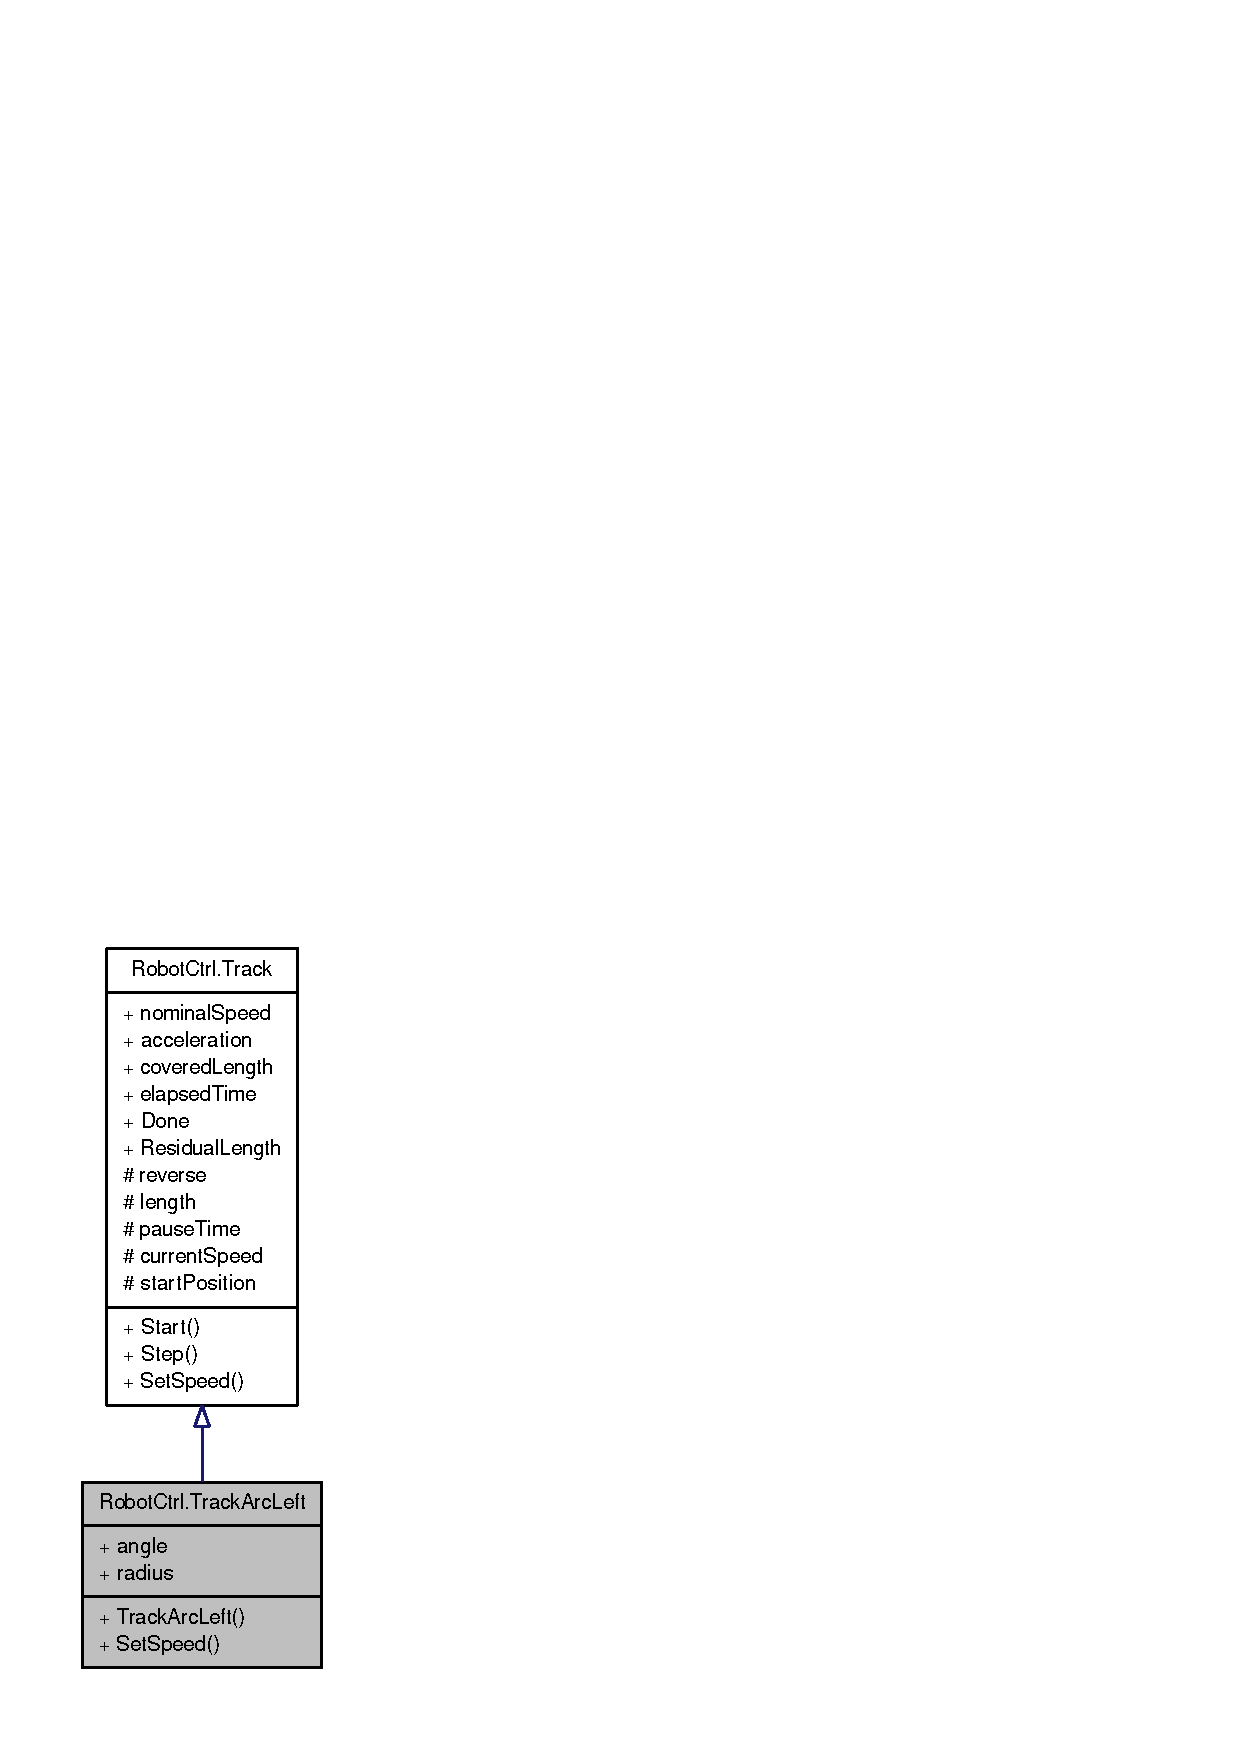
\includegraphics[width=158pt]{class_robot_ctrl_1_1_track_arc_left__inherit__graph}
\end{center}
\end{figure}


Zusammengehörigkeiten von RobotCtrl.TrackArcLeft:\nopagebreak
\begin{figure}[H]
\begin{center}
\leavevmode
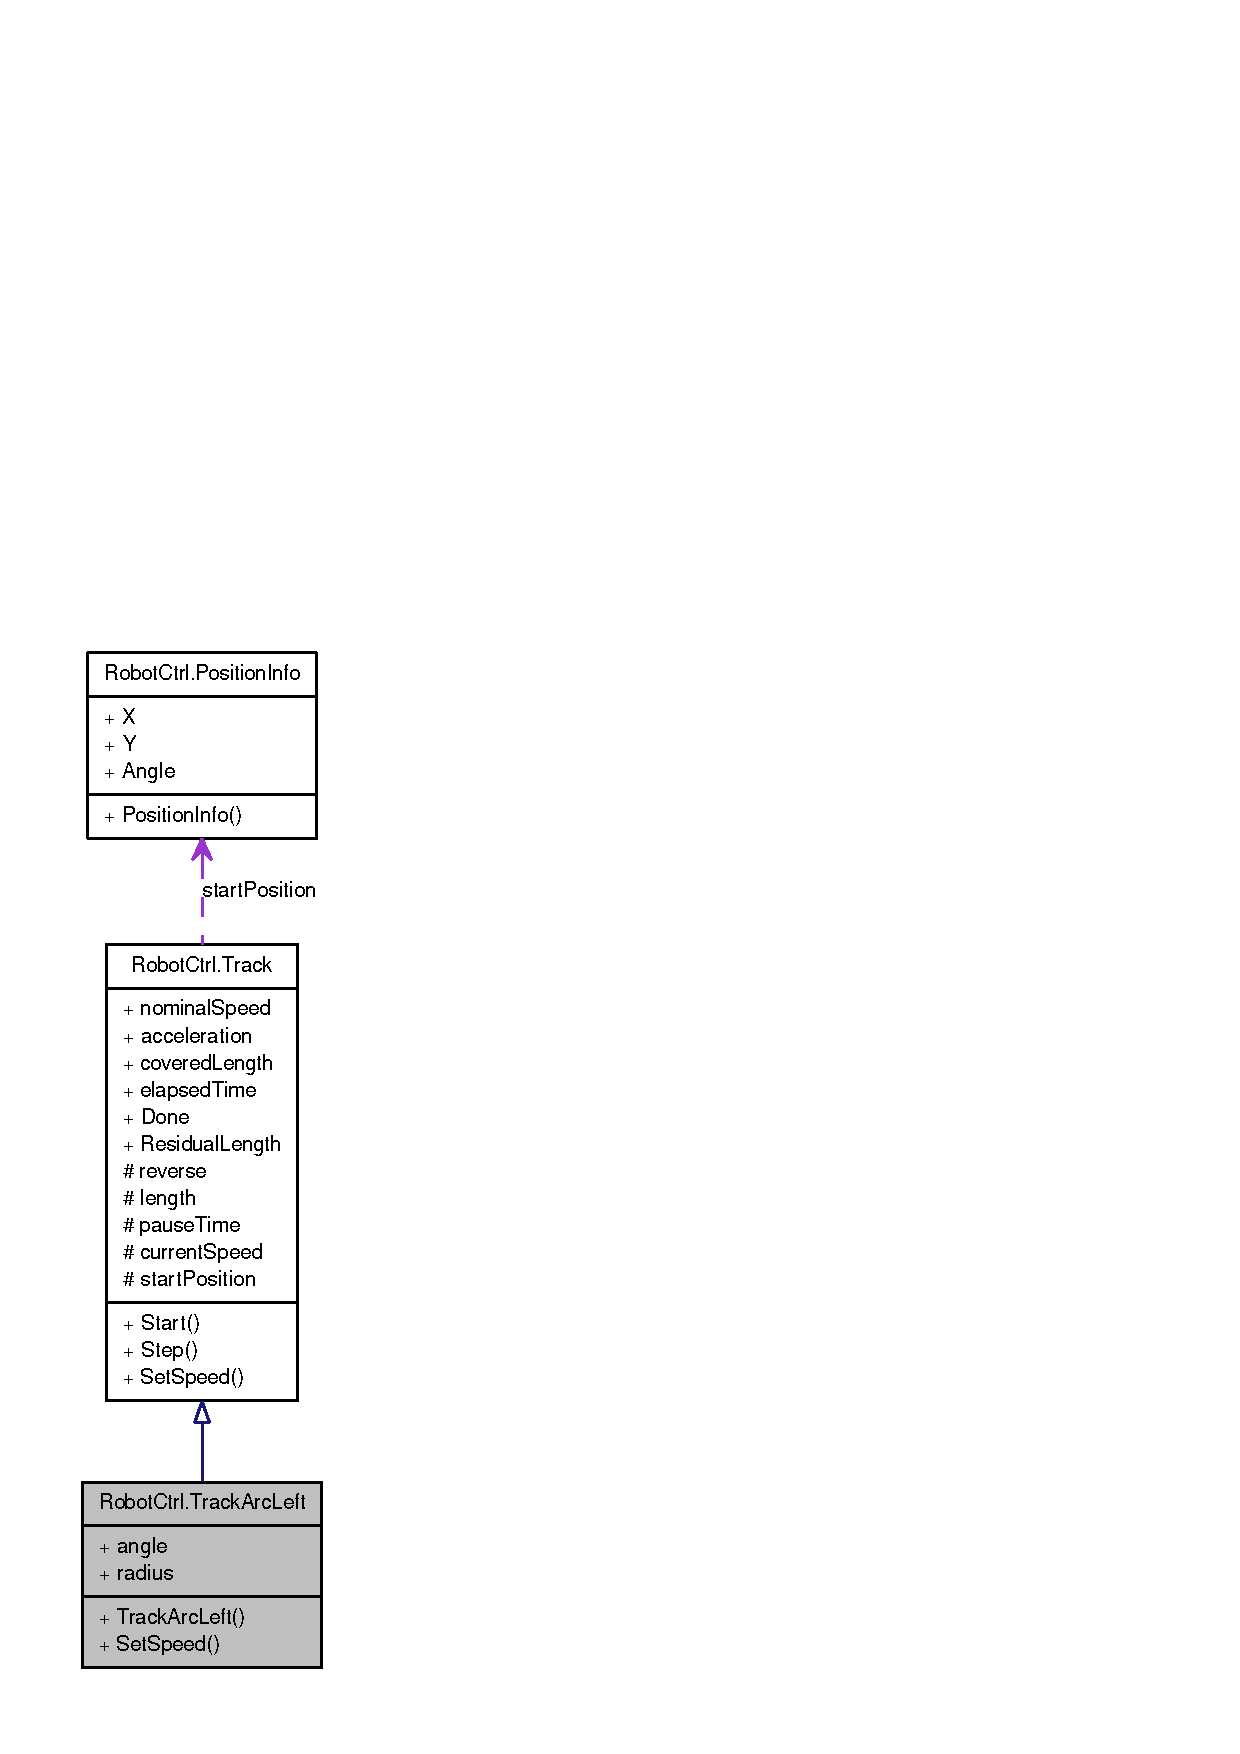
\includegraphics[height=400pt]{class_robot_ctrl_1_1_track_arc_left__coll__graph}
\end{center}
\end{figure}
\subsection*{Öffentliche Methoden}
\begin{DoxyCompactItemize}
\item 
\hyperlink{class_robot_ctrl_1_1_track_arc_left_a405f8fa89cf86603b3696a282d05dcff}{TrackArcLeft} (double radius, double angle, double speed, double acceleration)
\item 
override void \hyperlink{class_robot_ctrl_1_1_track_arc_left_aee8e8c1da176807436c2946e39bbd6ae}{SetSpeed} (double newSpeed, \hyperlink{class_robot_ctrl_1_1_motor_ctrl}{MotorCtrl} left, \hyperlink{class_robot_ctrl_1_1_motor_ctrl}{MotorCtrl} right)
\end{DoxyCompactItemize}
\subsection*{Öffentliche Attribute}
\begin{DoxyCompactItemize}
\item 
\hypertarget{class_robot_ctrl_1_1_track_arc_left_a3d6fadeb6e8d2967178696601569b3d5}{
double {\bfseries angle}}
\label{class_robot_ctrl_1_1_track_arc_left_a3d6fadeb6e8d2967178696601569b3d5}

\item 
\hypertarget{class_robot_ctrl_1_1_track_arc_left_a74198f81576aa2160802c31d1b37c9c8}{
double {\bfseries radius}}
\label{class_robot_ctrl_1_1_track_arc_left_a74198f81576aa2160802c31d1b37c9c8}

\end{DoxyCompactItemize}


\subsection{Ausführliche Beschreibung}
\hyperlink{class_robot_ctrl_1_1_track_arc_left}{TrackArcLeft} wird verwendet um einen Bogen nach links zu fahren. 

\subsection{Beschreibung der Konstruktoren und Destruktoren}
\hypertarget{class_robot_ctrl_1_1_track_arc_left_a405f8fa89cf86603b3696a282d05dcff}{
\index{RobotCtrl::TrackArcLeft@{RobotCtrl::TrackArcLeft}!TrackArcLeft@{TrackArcLeft}}
\index{TrackArcLeft@{TrackArcLeft}!RobotCtrl::TrackArcLeft@{RobotCtrl::TrackArcLeft}}
\subsubsection[{TrackArcLeft}]{\setlength{\rightskip}{0pt plus 5cm}RobotCtrl.TrackArcLeft.TrackArcLeft (double {\em radius}, \/  double {\em angle}, \/  double {\em speed}, \/  double {\em acceleration})}}
\label{class_robot_ctrl_1_1_track_arc_left_a405f8fa89cf86603b3696a282d05dcff}
Konstruktor \hyperlink{class_robot_ctrl_1_1_track_arc_left}{TrackArcLeft}


\begin{DoxyParams}{Parameter}
\item[{\em radius}]Radius f\"{u}r den Bogen  angle Winkel der abgefahren werden soll \item[{\em speed}]Geschwindigkeit mit der der Roboter fahren soll \item[{\em acceleration}]Beschleunigung auf dem Bogen \end{DoxyParams}


\subsection{Dokumentation der Elementfunktionen}
\hypertarget{class_robot_ctrl_1_1_track_arc_left_aee8e8c1da176807436c2946e39bbd6ae}{
\index{RobotCtrl::TrackArcLeft@{RobotCtrl::TrackArcLeft}!SetSpeed@{SetSpeed}}
\index{SetSpeed@{SetSpeed}!RobotCtrl::TrackArcLeft@{RobotCtrl::TrackArcLeft}}
\subsubsection[{SetSpeed}]{\setlength{\rightskip}{0pt plus 5cm}override void RobotCtrl.TrackArcLeft.SetSpeed (double {\em newSpeed}, \/  {\bf MotorCtrl} {\em left}, \/  {\bf MotorCtrl} {\em right})\hspace{0.3cm}{\ttfamily  \mbox{[}virtual\mbox{]}}}}
\label{class_robot_ctrl_1_1_track_arc_left_aee8e8c1da176807436c2946e39bbd6ae}
\"{U}berschreibt die SetSpeed Methode der Basisklasse \hyperlink{class_robot_ctrl_1_1_track}{Track}


\begin{DoxyParams}{Parameter}
\item[{\em newSpeed}]Setzt die neue Geschwindigkeit \item[{\em left}]Referenz auf den linken Motor \item[{\em right}]Referenz auf den rechten Motor \end{DoxyParams}


Erneute Implementation von \hyperlink{class_robot_ctrl_1_1_track_a9abc3ccf4bf1d9db8d461f2cb4b4b0d3}{RobotCtrl.Track}.



Die Dokumentation für diese Klasse wurde erzeugt aufgrund der Datei:\begin{DoxyCompactItemize}
\item 
Track.cs\end{DoxyCompactItemize}

\hypertarget{class_robot_ctrl_1_1_track_arc_right}{
\section{RobotCtrl.TrackArcRight Klassenreferenz}
\label{class_robot_ctrl_1_1_track_arc_right}\index{RobotCtrl::TrackArcRight@{RobotCtrl::TrackArcRight}}
}


\hyperlink{class_robot_ctrl_1_1_track_arc_right}{TrackArcRight} wird verwendet um einen Bogen nach rechts zu fahren.  




Klassendiagramm für RobotCtrl.TrackArcRight:

Zusammengehörigkeiten von RobotCtrl.TrackArcRight:\subsection*{Öffentliche Methoden}
\begin{DoxyCompactItemize}
\item 
\hyperlink{class_robot_ctrl_1_1_track_arc_right_a54609ff71d77c37e9423cae42de7c347}{TrackArcRight} (double radius, double angle, double speed, double acceleration)
\item 
override void \hyperlink{class_robot_ctrl_1_1_track_arc_right_a7b2db0d3709e4919da0645a6713a87bb}{SetSpeed} (double newSpeed, \hyperlink{class_robot_ctrl_1_1_motor_ctrl}{MotorCtrl} left, \hyperlink{class_robot_ctrl_1_1_motor_ctrl}{MotorCtrl} right)
\end{DoxyCompactItemize}
\subsection*{Öffentliche Attribute}
\begin{DoxyCompactItemize}
\item 
\hypertarget{class_robot_ctrl_1_1_track_arc_right_a6e5fa9d8296e05e45d3db261997e224e}{
double {\bfseries angle}}
\label{class_robot_ctrl_1_1_track_arc_right_a6e5fa9d8296e05e45d3db261997e224e}

\item 
\hypertarget{class_robot_ctrl_1_1_track_arc_right_a499b381000fccf8f8c3af0ea1940a996}{
double {\bfseries radius}}
\label{class_robot_ctrl_1_1_track_arc_right_a499b381000fccf8f8c3af0ea1940a996}

\end{DoxyCompactItemize}


\subsection{Ausführliche Beschreibung}
\hyperlink{class_robot_ctrl_1_1_track_arc_right}{TrackArcRight} wird verwendet um einen Bogen nach rechts zu fahren. 

\subsection{Beschreibung der Konstruktoren und Destruktoren}
\hypertarget{class_robot_ctrl_1_1_track_arc_right_a54609ff71d77c37e9423cae42de7c347}{
\index{RobotCtrl::TrackArcRight@{RobotCtrl::TrackArcRight}!TrackArcRight@{TrackArcRight}}
\index{TrackArcRight@{TrackArcRight}!RobotCtrl::TrackArcRight@{RobotCtrl::TrackArcRight}}
\subsubsection[{TrackArcRight}]{\setlength{\rightskip}{0pt plus 5cm}RobotCtrl.TrackArcRight.TrackArcRight (double {\em radius}, \/  double {\em angle}, \/  double {\em speed}, \/  double {\em acceleration})}}
\label{class_robot_ctrl_1_1_track_arc_right_a54609ff71d77c37e9423cae42de7c347}
Konstruktor \hyperlink{class_robot_ctrl_1_1_track_arc_right}{TrackArcRight}


\begin{DoxyParams}{Parameter}
\item[{\em radius}]Radius f\"{u}r den Bogen  angle Winkel der abgefahren werden soll \item[{\em speed}]Geschwindigkeit mit der der Roboter fahren soll \item[{\em acceleration}]Beschleunigung auf dem Bogen \end{DoxyParams}


\subsection{Dokumentation der Elementfunktionen}
\hypertarget{class_robot_ctrl_1_1_track_arc_right_a7b2db0d3709e4919da0645a6713a87bb}{
\index{RobotCtrl::TrackArcRight@{RobotCtrl::TrackArcRight}!SetSpeed@{SetSpeed}}
\index{SetSpeed@{SetSpeed}!RobotCtrl::TrackArcRight@{RobotCtrl::TrackArcRight}}
\subsubsection[{SetSpeed}]{\setlength{\rightskip}{0pt plus 5cm}override void RobotCtrl.TrackArcRight.SetSpeed (double {\em newSpeed}, \/  {\bf MotorCtrl} {\em left}, \/  {\bf MotorCtrl} {\em right})\hspace{0.3cm}{\ttfamily  \mbox{[}virtual\mbox{]}}}}
\label{class_robot_ctrl_1_1_track_arc_right_a7b2db0d3709e4919da0645a6713a87bb}
\"{U}berschreibt die SetSpeed Methode der Basisklasse \hyperlink{class_robot_ctrl_1_1_track}{Track}


\begin{DoxyParams}{Parameter}
\item[{\em newSpeed}]Setzt die neue Geschwindigkeit \item[{\em left}]Referenz auf den linken Motor \item[{\em right}]Referenz auf den rechten Motor \end{DoxyParams}


Erneute Implementation von \hyperlink{class_robot_ctrl_1_1_track_a9abc3ccf4bf1d9db8d461f2cb4b4b0d3}{RobotCtrl.Track}.



Die Dokumentation für diese Klasse wurde erzeugt aufgrund der Datei:\begin{DoxyCompactItemize}
\item 
Track.cs\end{DoxyCompactItemize}

\hypertarget{class_robot_ctrl_1_1_track_contour_left}{
\section{RobotCtrl.TrackContourLeft Klassenreferenz}
\label{class_robot_ctrl_1_1_track_contour_left}\index{RobotCtrl::TrackContourLeft@{RobotCtrl::TrackContourLeft}}
}


\hyperlink{class_robot_ctrl_1_1_track_contour_left}{TrackContourLeft} wird verwendet um eine Kontur linksherum abzufahren.  




Klassendiagramm für RobotCtrl.TrackContourLeft:\nopagebreak
\begin{figure}[H]
\begin{center}
\leavevmode
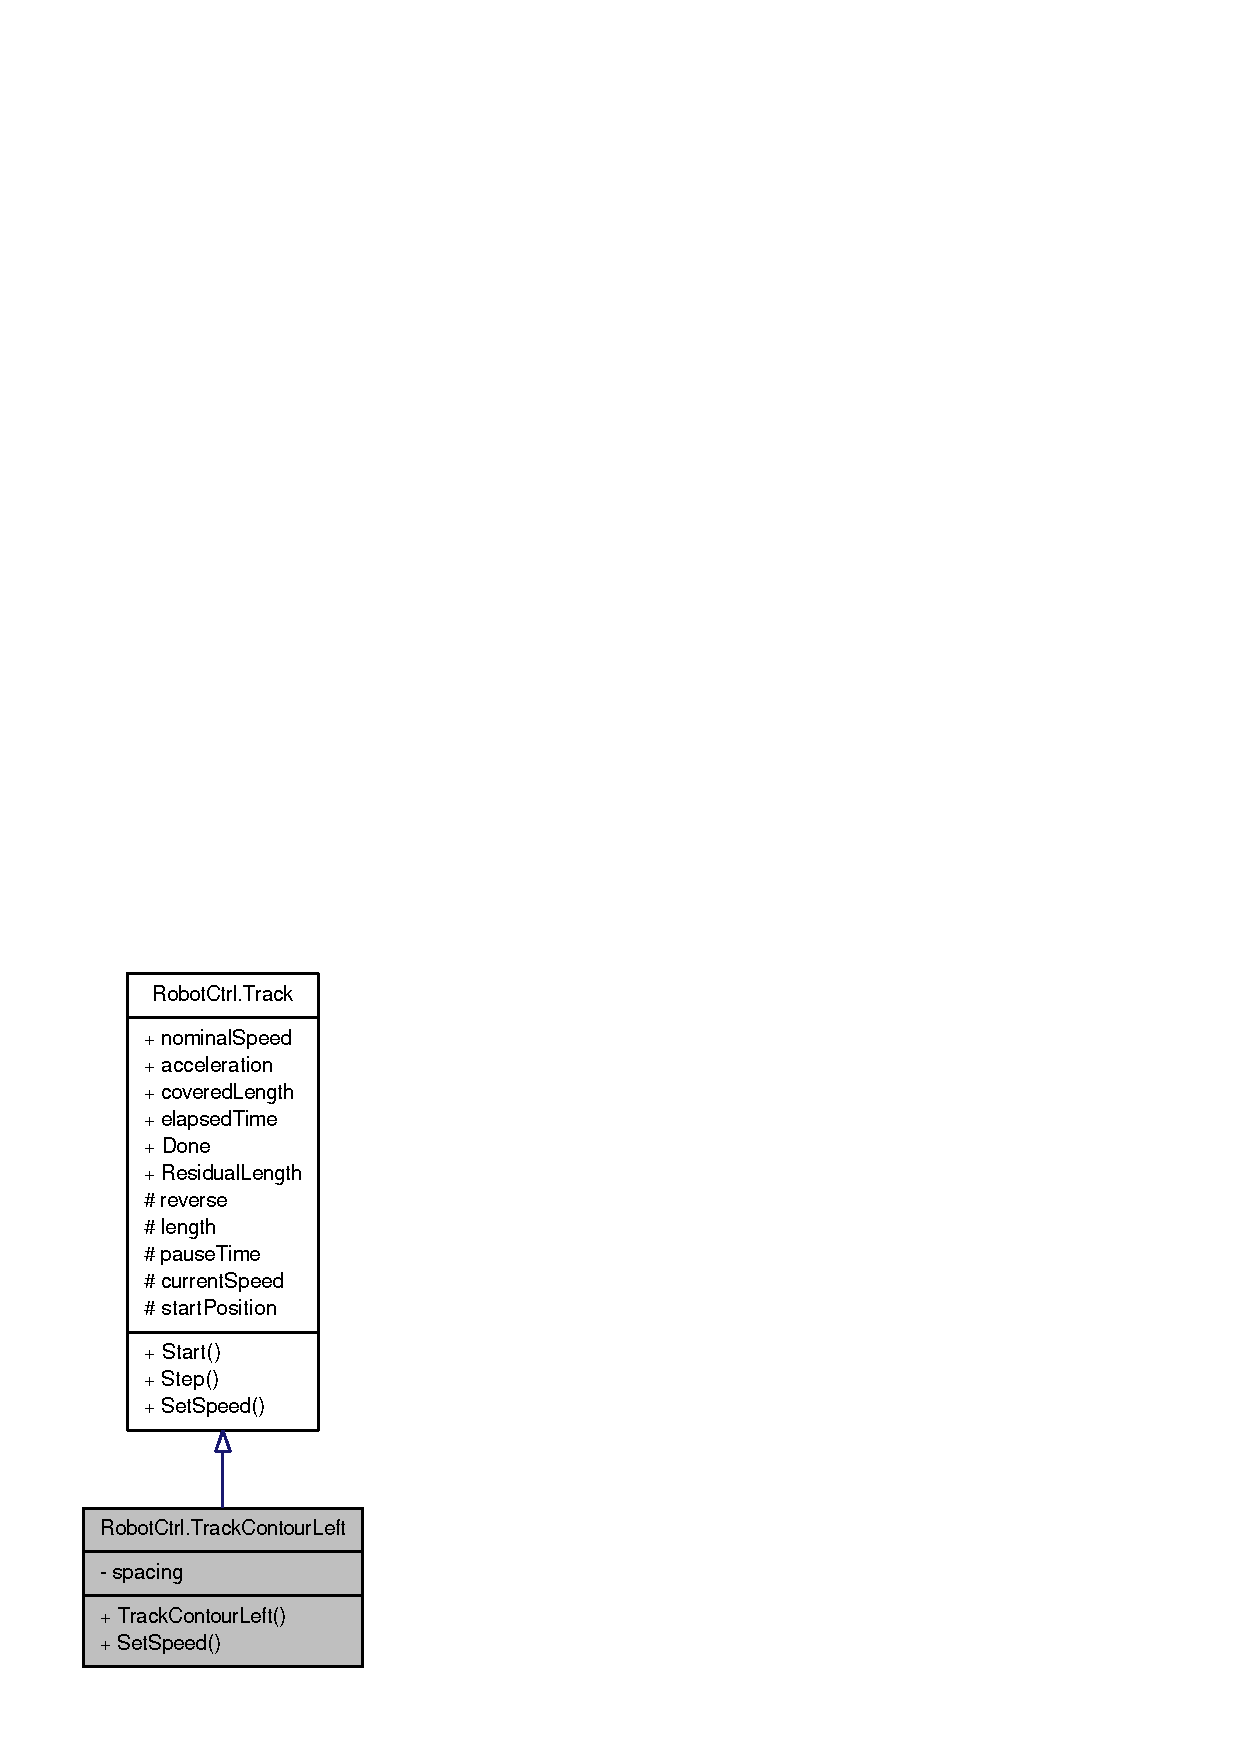
\includegraphics[width=178pt]{class_robot_ctrl_1_1_track_contour_left__inherit__graph}
\end{center}
\end{figure}


Zusammengehörigkeiten von RobotCtrl.TrackContourLeft:\nopagebreak
\begin{figure}[H]
\begin{center}
\leavevmode
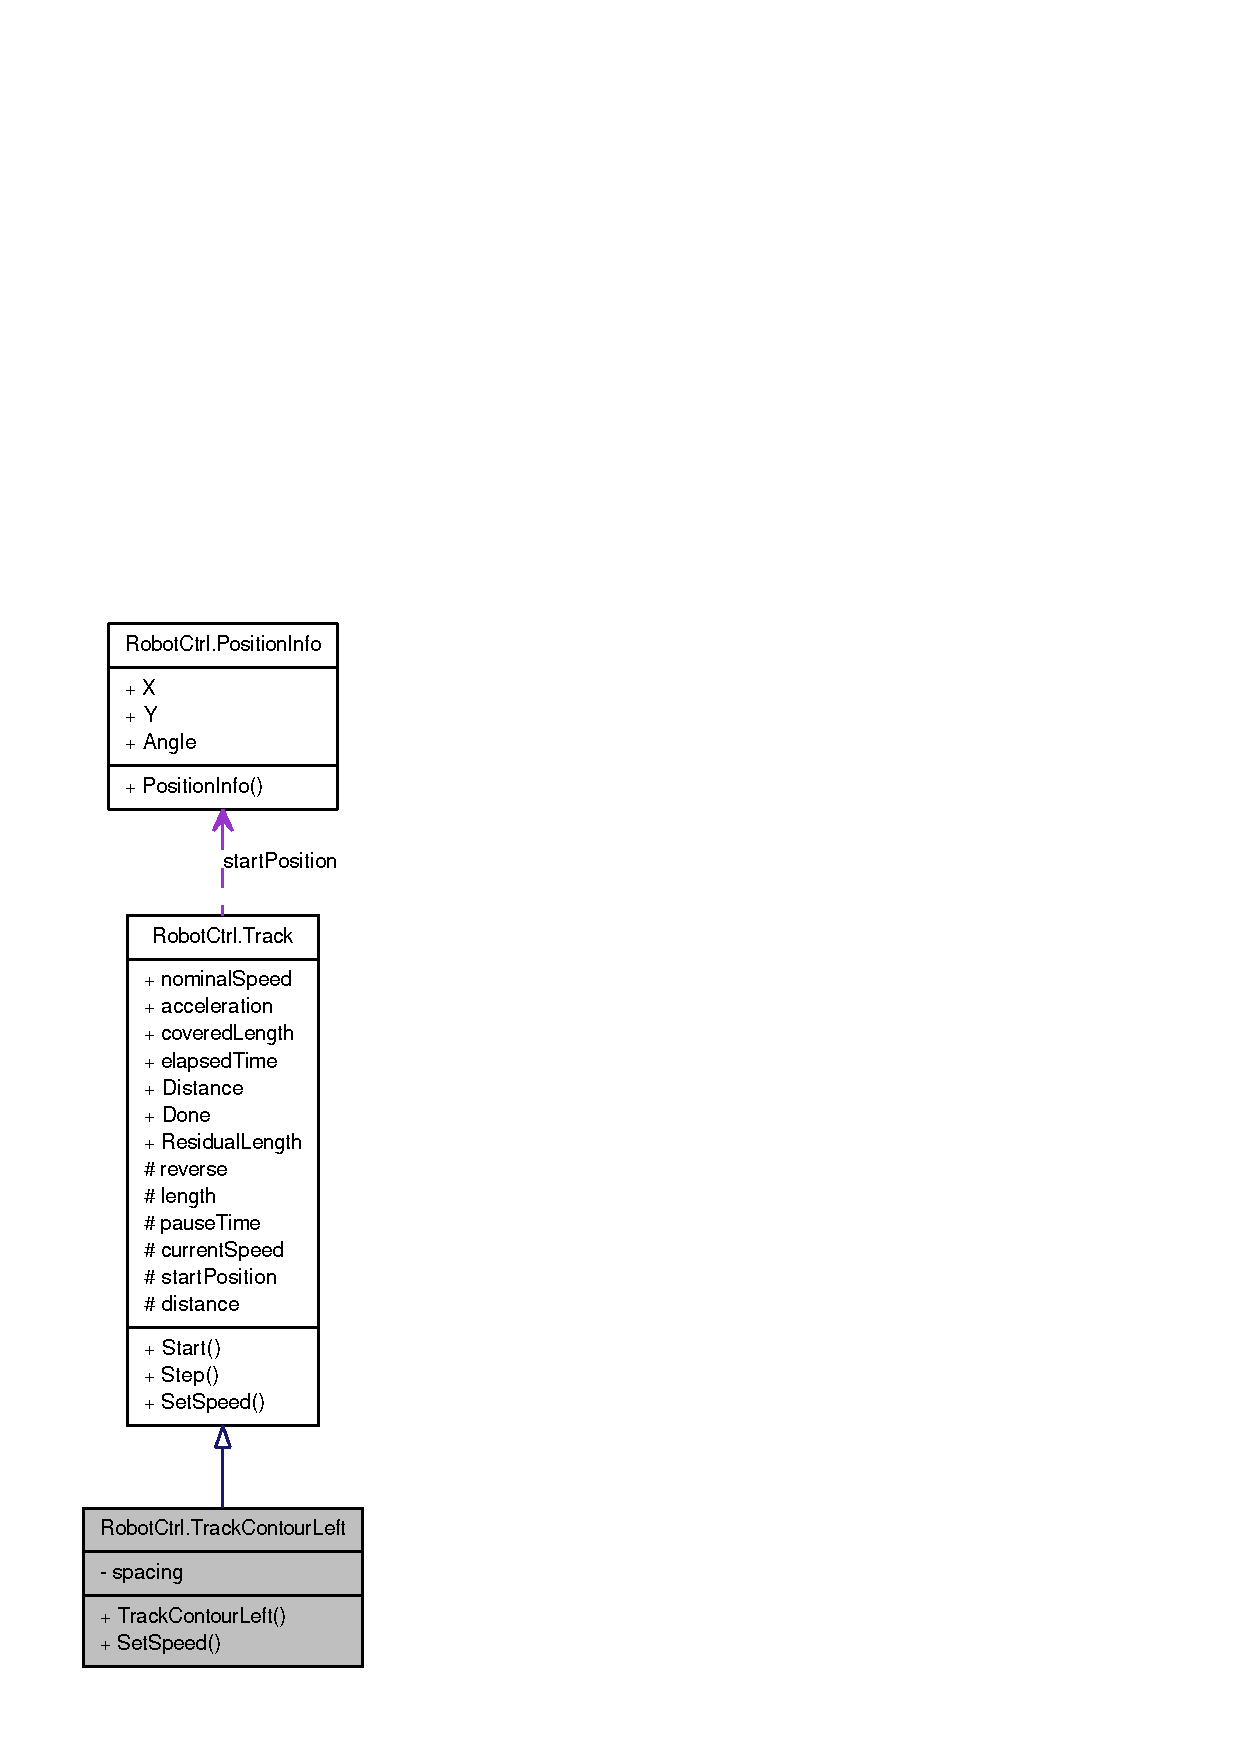
\includegraphics[height=400pt]{class_robot_ctrl_1_1_track_contour_left__coll__graph}
\end{center}
\end{figure}
\subsection*{Öffentliche Methoden}
\begin{DoxyCompactItemize}
\item 
\hyperlink{class_robot_ctrl_1_1_track_contour_left_a73c01532abc01420c2a35bea80be194d}{TrackContourLeft} (double spacing, double speed, double acceleration)
\item 
override void \hyperlink{class_robot_ctrl_1_1_track_contour_left_ae7938250af614625cd08a498c0f15195}{SetSpeed} (double newSpeed, \hyperlink{class_robot_ctrl_1_1_motor_ctrl}{MotorCtrl} left, \hyperlink{class_robot_ctrl_1_1_motor_ctrl}{MotorCtrl} right)
\end{DoxyCompactItemize}


\subsection{Ausführliche Beschreibung}
\hyperlink{class_robot_ctrl_1_1_track_contour_left}{TrackContourLeft} wird verwendet um eine Kontur linksherum abzufahren. 

\subsection{Beschreibung der Konstruktoren und Destruktoren}
\hypertarget{class_robot_ctrl_1_1_track_contour_left_a73c01532abc01420c2a35bea80be194d}{
\index{RobotCtrl::TrackContourLeft@{RobotCtrl::TrackContourLeft}!TrackContourLeft@{TrackContourLeft}}
\index{TrackContourLeft@{TrackContourLeft}!RobotCtrl::TrackContourLeft@{RobotCtrl::TrackContourLeft}}
\subsubsection[{TrackContourLeft}]{\setlength{\rightskip}{0pt plus 5cm}RobotCtrl.TrackContourLeft.TrackContourLeft (double {\em spacing}, \/  double {\em speed}, \/  double {\em acceleration})}}
\label{class_robot_ctrl_1_1_track_contour_left_a73c01532abc01420c2a35bea80be194d}
Konstruktor \hyperlink{class_robot_ctrl_1_1_track_contour_left}{TrackContourLeft}

spacing Abstand zur Kontur 
\begin{DoxyParams}{Parameter}
\item[{\em speed}]Geschwindigkeit mit der der Roboter fahren soll \item[{\em acceleration}]Beschleunigung auf dem Weg um die Kontur \end{DoxyParams}


\subsection{Dokumentation der Elementfunktionen}
\hypertarget{class_robot_ctrl_1_1_track_contour_left_ae7938250af614625cd08a498c0f15195}{
\index{RobotCtrl::TrackContourLeft@{RobotCtrl::TrackContourLeft}!SetSpeed@{SetSpeed}}
\index{SetSpeed@{SetSpeed}!RobotCtrl::TrackContourLeft@{RobotCtrl::TrackContourLeft}}
\subsubsection[{SetSpeed}]{\setlength{\rightskip}{0pt plus 5cm}override void RobotCtrl.TrackContourLeft.SetSpeed (double {\em newSpeed}, \/  {\bf MotorCtrl} {\em left}, \/  {\bf MotorCtrl} {\em right})\hspace{0.3cm}{\ttfamily  \mbox{[}virtual\mbox{]}}}}
\label{class_robot_ctrl_1_1_track_contour_left_ae7938250af614625cd08a498c0f15195}
\"{U}berschreibt die SetSpeed Methode der Basisklasse \hyperlink{class_robot_ctrl_1_1_track}{Track}


\begin{DoxyParams}{Parameter}
\item[{\em newSpeed}]Setzt die neue Geschwindigkeit \item[{\em left}]Referenz auf den linken Motor \item[{\em right}]Referenz auf den rechten Motor \end{DoxyParams}


Erneute Implementation von \hyperlink{class_robot_ctrl_1_1_track_a9abc3ccf4bf1d9db8d461f2cb4b4b0d3}{RobotCtrl.Track}.



Die Dokumentation für diese Klasse wurde erzeugt aufgrund der Datei:\begin{DoxyCompactItemize}
\item 
Track.cs\end{DoxyCompactItemize}

\hypertarget{class_robot_ctrl_1_1_track_line}{
\section{RobotCtrl.TrackLine Klassenreferenz}
\label{class_robot_ctrl_1_1_track_line}\index{RobotCtrl::TrackLine@{RobotCtrl::TrackLine}}
}


\hyperlink{class_robot_ctrl_1_1_track_line}{TrackLine} wird verwendet um eine gerade Strecke abzufahren.  




Klassendiagramm für RobotCtrl.TrackLine:

Zusammengehörigkeiten von RobotCtrl.TrackLine:\subsection*{Öffentliche Methoden}
\begin{DoxyCompactItemize}
\item 
\hyperlink{class_robot_ctrl_1_1_track_line_ab4ab93433f36792a4748322b94febfc7}{TrackLine} (double length, double speed, double acceleration)
\item 
override void \hyperlink{class_robot_ctrl_1_1_track_line_ad73ae0e8f7aea1765834ab90f5bd6b23}{SetSpeed} (double newSpeed, \hyperlink{class_robot_ctrl_1_1_motor_ctrl}{MotorCtrl} left, \hyperlink{class_robot_ctrl_1_1_motor_ctrl}{MotorCtrl} right)
\end{DoxyCompactItemize}


\subsection{Ausführliche Beschreibung}
\hyperlink{class_robot_ctrl_1_1_track_line}{TrackLine} wird verwendet um eine gerade Strecke abzufahren. 

\subsection{Beschreibung der Konstruktoren und Destruktoren}
\hypertarget{class_robot_ctrl_1_1_track_line_ab4ab93433f36792a4748322b94febfc7}{
\index{RobotCtrl::TrackLine@{RobotCtrl::TrackLine}!TrackLine@{TrackLine}}
\index{TrackLine@{TrackLine}!RobotCtrl::TrackLine@{RobotCtrl::TrackLine}}
\subsubsection[{TrackLine}]{\setlength{\rightskip}{0pt plus 5cm}RobotCtrl.TrackLine.TrackLine (double {\em length}, \/  double {\em speed}, \/  double {\em acceleration})}}
\label{class_robot_ctrl_1_1_track_line_ab4ab93433f36792a4748322b94febfc7}
Konstruktor \hyperlink{class_robot_ctrl_1_1_track_line}{TrackLine}


\begin{DoxyParams}{Parameter}
\item[{\em length}]L\"{a}nge der Strecke \item[{\em speed}]Geschwindigkeit \item[{\em acceleration}]Beschleunigung \end{DoxyParams}


\subsection{Dokumentation der Elementfunktionen}
\hypertarget{class_robot_ctrl_1_1_track_line_ad73ae0e8f7aea1765834ab90f5bd6b23}{
\index{RobotCtrl::TrackLine@{RobotCtrl::TrackLine}!SetSpeed@{SetSpeed}}
\index{SetSpeed@{SetSpeed}!RobotCtrl::TrackLine@{RobotCtrl::TrackLine}}
\subsubsection[{SetSpeed}]{\setlength{\rightskip}{0pt plus 5cm}override void RobotCtrl.TrackLine.SetSpeed (double {\em newSpeed}, \/  {\bf MotorCtrl} {\em left}, \/  {\bf MotorCtrl} {\em right})\hspace{0.3cm}{\ttfamily  \mbox{[}virtual\mbox{]}}}}
\label{class_robot_ctrl_1_1_track_line_ad73ae0e8f7aea1765834ab90f5bd6b23}
\"{U}berschreibt die SetSpeed Methode der Basisklasse \hyperlink{class_robot_ctrl_1_1_track}{Track}


\begin{DoxyParams}{Parameter}
\item[{\em newSpeed}]Setzt die neue Geschwindigkeit \item[{\em left}]Referenz auf den linken Motor \item[{\em right}]Referenz auf den rechten Motor \end{DoxyParams}


Erneute Implementation von \hyperlink{class_robot_ctrl_1_1_track_a9abc3ccf4bf1d9db8d461f2cb4b4b0d3}{RobotCtrl.Track}.



Die Dokumentation für diese Klasse wurde erzeugt aufgrund der Datei:\begin{DoxyCompactItemize}
\item 
Track.cs\end{DoxyCompactItemize}

\hypertarget{class_robot_ctrl_1_1_track_pause}{
\section{RobotCtrl.TrackPause Klassenreferenz}
\label{class_robot_ctrl_1_1_track_pause}\index{RobotCtrl::TrackPause@{RobotCtrl::TrackPause}}
}


\hyperlink{class_robot_ctrl_1_1_track_pause}{TrackPause} wird verwendet um einen eine vorgegebene Zeit zu warten.  




Klassendiagramm für RobotCtrl.TrackPause:\nopagebreak
\begin{figure}[H]
\begin{center}
\leavevmode
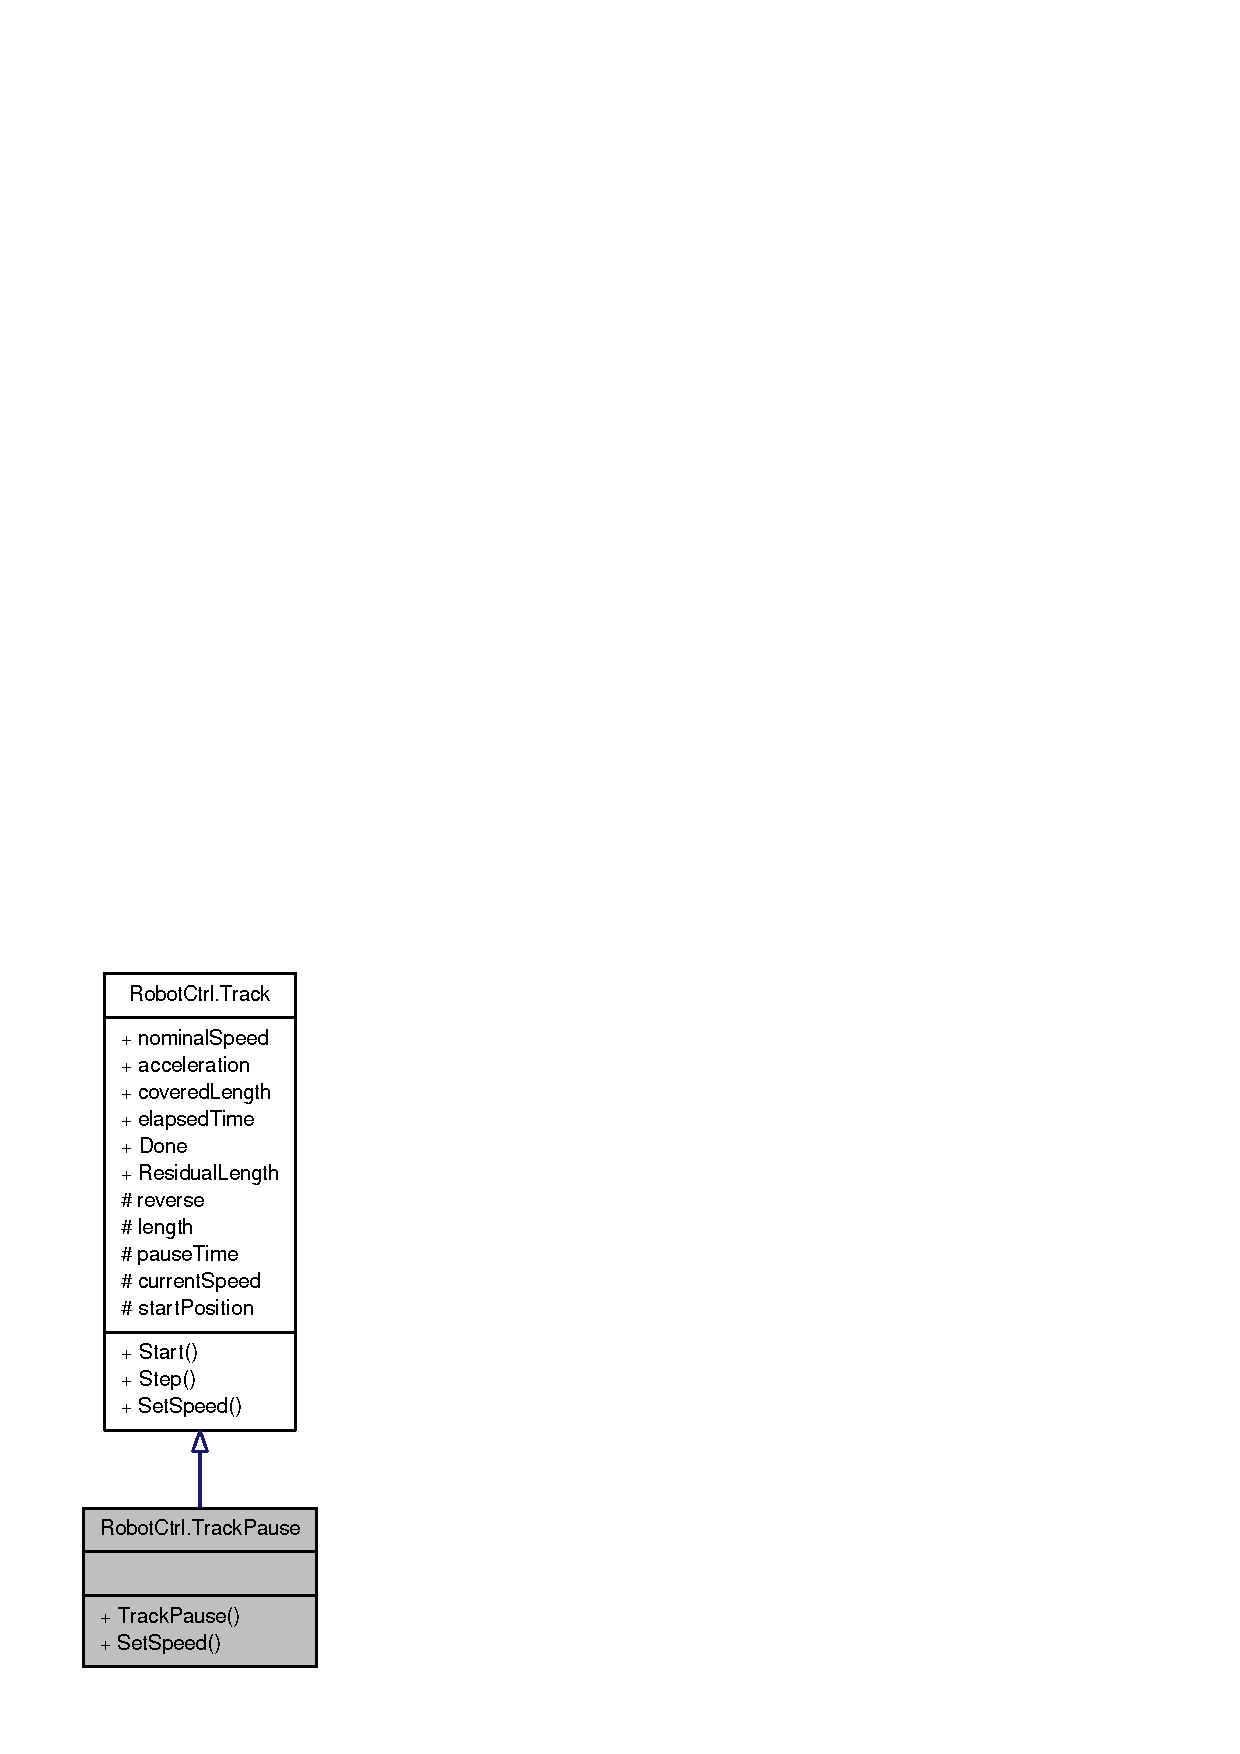
\includegraphics[height=400pt]{class_robot_ctrl_1_1_track_pause__inherit__graph}
\end{center}
\end{figure}


Zusammengehörigkeiten von RobotCtrl.TrackPause:\nopagebreak
\begin{figure}[H]
\begin{center}
\leavevmode
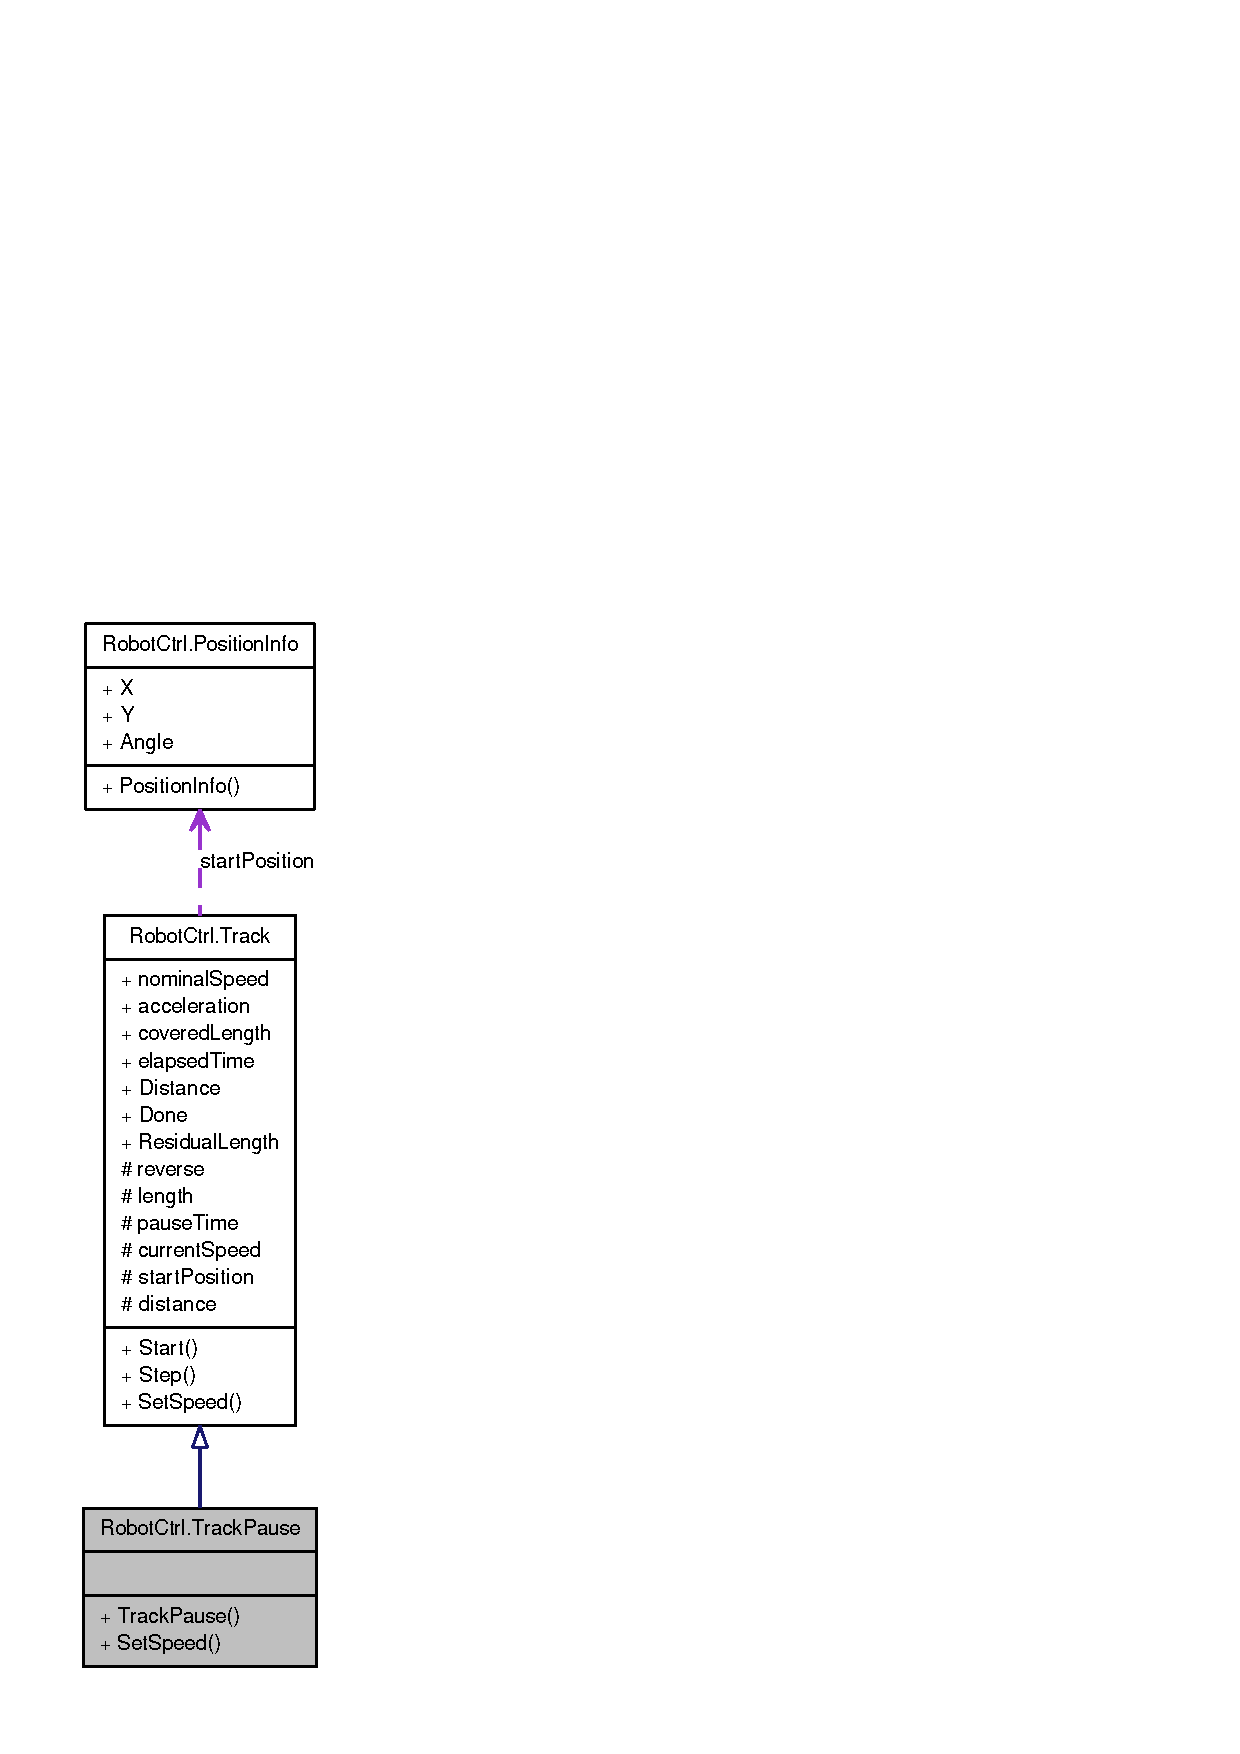
\includegraphics[height=400pt]{class_robot_ctrl_1_1_track_pause__coll__graph}
\end{center}
\end{figure}
\subsection*{Öffentliche Methoden}
\begin{DoxyCompactItemize}
\item 
\hyperlink{class_robot_ctrl_1_1_track_pause_ab869a1e5eb8a5db402ad7a7515700688}{TrackPause} (double pauseTimeSeconds)
\item 
override void \hyperlink{class_robot_ctrl_1_1_track_pause_a47133c69e455aa2c04f1bc3a6b5999b6}{SetSpeed} (double newSpeed, \hyperlink{class_robot_ctrl_1_1_motor_ctrl}{MotorCtrl} left, \hyperlink{class_robot_ctrl_1_1_motor_ctrl}{MotorCtrl} right)
\end{DoxyCompactItemize}


\subsection{Ausführliche Beschreibung}
\hyperlink{class_robot_ctrl_1_1_track_pause}{TrackPause} wird verwendet um einen eine vorgegebene Zeit zu warten. 

\subsection{Beschreibung der Konstruktoren und Destruktoren}
\hypertarget{class_robot_ctrl_1_1_track_pause_ab869a1e5eb8a5db402ad7a7515700688}{
\index{RobotCtrl::TrackPause@{RobotCtrl::TrackPause}!TrackPause@{TrackPause}}
\index{TrackPause@{TrackPause}!RobotCtrl::TrackPause@{RobotCtrl::TrackPause}}
\subsubsection[{TrackPause}]{\setlength{\rightskip}{0pt plus 5cm}RobotCtrl.TrackPause.TrackPause (double {\em pauseTimeSeconds})}}
\label{class_robot_ctrl_1_1_track_pause_ab869a1e5eb8a5db402ad7a7515700688}
Konstruktor \hyperlink{class_robot_ctrl_1_1_track_pause}{TrackPause}


\begin{DoxyParams}{Parameter}
\item[{\em pauseTimeSeconds}]Zeit in Sekunden \end{DoxyParams}


\subsection{Dokumentation der Elementfunktionen}
\hypertarget{class_robot_ctrl_1_1_track_pause_a47133c69e455aa2c04f1bc3a6b5999b6}{
\index{RobotCtrl::TrackPause@{RobotCtrl::TrackPause}!SetSpeed@{SetSpeed}}
\index{SetSpeed@{SetSpeed}!RobotCtrl::TrackPause@{RobotCtrl::TrackPause}}
\subsubsection[{SetSpeed}]{\setlength{\rightskip}{0pt plus 5cm}override void RobotCtrl.TrackPause.SetSpeed (double {\em newSpeed}, \/  {\bf MotorCtrl} {\em left}, \/  {\bf MotorCtrl} {\em right})\hspace{0.3cm}{\ttfamily  \mbox{[}virtual\mbox{]}}}}
\label{class_robot_ctrl_1_1_track_pause_a47133c69e455aa2c04f1bc3a6b5999b6}
\"{U}berschreibt die SetSpeed Methode der Basisklasse \hyperlink{class_robot_ctrl_1_1_track}{Track}


\begin{DoxyParams}{Parameter}
\item[{\em newSpeed}]Setzt die neue Geschwindigkeit \item[{\em left}]Referenz auf den linken Motor \item[{\em right}]Referenz auf den rechten Motor \end{DoxyParams}


Erneute Implementation von \hyperlink{class_robot_ctrl_1_1_track_a9abc3ccf4bf1d9db8d461f2cb4b4b0d3}{RobotCtrl.Track}.



Die Dokumentation für diese Klasse wurde erzeugt aufgrund der Datei:\begin{DoxyCompactItemize}
\item 
Track.cs\end{DoxyCompactItemize}

\hypertarget{class_robot_ctrl_1_1_track_turn}{
\section{RobotCtrl.TrackTurn Klassenreferenz}
\label{class_robot_ctrl_1_1_track_turn}\index{RobotCtrl::TrackTurn@{RobotCtrl::TrackTurn}}
}


\hyperlink{class_robot_ctrl_1_1_track_turn}{TrackTurn} wird verwendet um sich um die eigene Achse zu drehen.  




Klassendiagramm für RobotCtrl.TrackTurn:\nopagebreak
\begin{figure}[H]
\begin{center}
\leavevmode
\includegraphics[height=400pt]{class_robot_ctrl_1_1_track_turn__inherit__graph}
\end{center}
\end{figure}


Zusammengehörigkeiten von RobotCtrl.TrackTurn:\nopagebreak
\begin{figure}[H]
\begin{center}
\leavevmode
\includegraphics[height=400pt]{class_robot_ctrl_1_1_track_turn__coll__graph}
\end{center}
\end{figure}
\subsection*{Öffentliche Methoden}
\begin{DoxyCompactItemize}
\item 
\hyperlink{class_robot_ctrl_1_1_track_turn_a734b50f5f72a3521d15855b0f86d2c6c}{TrackTurn} (double angle, double speed, double acceleration)
\item 
override void \hyperlink{class_robot_ctrl_1_1_track_turn_a065e23cd313e746cb65496c9b9df0955}{SetSpeed} (double newSpeed, \hyperlink{class_robot_ctrl_1_1_motor_ctrl}{MotorCtrl} left, \hyperlink{class_robot_ctrl_1_1_motor_ctrl}{MotorCtrl} right)
\end{DoxyCompactItemize}
\subsection*{Öffentliche Attribute}
\begin{DoxyCompactItemize}
\item 
\hypertarget{class_robot_ctrl_1_1_track_turn_a5ea004969a5701516952d1424dfa2be3}{
double {\bfseries angle}}
\label{class_robot_ctrl_1_1_track_turn_a5ea004969a5701516952d1424dfa2be3}

\end{DoxyCompactItemize}


\subsection{Ausführliche Beschreibung}
\hyperlink{class_robot_ctrl_1_1_track_turn}{TrackTurn} wird verwendet um sich um die eigene Achse zu drehen. 

\subsection{Beschreibung der Konstruktoren und Destruktoren}
\hypertarget{class_robot_ctrl_1_1_track_turn_a734b50f5f72a3521d15855b0f86d2c6c}{
\index{RobotCtrl::TrackTurn@{RobotCtrl::TrackTurn}!TrackTurn@{TrackTurn}}
\index{TrackTurn@{TrackTurn}!RobotCtrl::TrackTurn@{RobotCtrl::TrackTurn}}
\subsubsection[{TrackTurn}]{\setlength{\rightskip}{0pt plus 5cm}RobotCtrl.TrackTurn.TrackTurn (double {\em angle}, \/  double {\em speed}, \/  double {\em acceleration})}}
\label{class_robot_ctrl_1_1_track_turn_a734b50f5f72a3521d15855b0f86d2c6c}
Konstruktor \hyperlink{class_robot_ctrl_1_1_track_turn}{TrackTurn}

angle Winkel um den gedreht werden soll 
\begin{DoxyParams}{Parameter}
\item[{\em speed}]Geschwindigkeit mit der der Roboter sich drehen soll \item[{\em acceleration}]Beschleunigung f\"{u}r die Drehung \end{DoxyParams}


\subsection{Dokumentation der Elementfunktionen}
\hypertarget{class_robot_ctrl_1_1_track_turn_a065e23cd313e746cb65496c9b9df0955}{
\index{RobotCtrl::TrackTurn@{RobotCtrl::TrackTurn}!SetSpeed@{SetSpeed}}
\index{SetSpeed@{SetSpeed}!RobotCtrl::TrackTurn@{RobotCtrl::TrackTurn}}
\subsubsection[{SetSpeed}]{\setlength{\rightskip}{0pt plus 5cm}override void RobotCtrl.TrackTurn.SetSpeed (double {\em newSpeed}, \/  {\bf MotorCtrl} {\em left}, \/  {\bf MotorCtrl} {\em right})\hspace{0.3cm}{\ttfamily  \mbox{[}virtual\mbox{]}}}}
\label{class_robot_ctrl_1_1_track_turn_a065e23cd313e746cb65496c9b9df0955}
\"{U}berschreibt die SetSpeed Methode der Basisklasse \hyperlink{class_robot_ctrl_1_1_track}{Track}


\begin{DoxyParams}{Parameter}
\item[{\em newSpeed}]Setzt die neue Geschwindigkeit \item[{\em left}]Referenz auf den linken Motor \item[{\em right}]Referenz auf den rechten Motor \end{DoxyParams}


Erneute Implementation von \hyperlink{class_robot_ctrl_1_1_track_a9abc3ccf4bf1d9db8d461f2cb4b4b0d3}{RobotCtrl.Track}.



Die Dokumentation für diese Klasse wurde erzeugt aufgrund der Datei:\begin{DoxyCompactItemize}
\item 
Track.cs\end{DoxyCompactItemize}

\hypertarget{class_world_view_1_1_world_view}{
\section{WorldView.WorldView Klassenreferenz}
\label{class_world_view_1_1_world_view}\index{WorldView::WorldView@{WorldView::WorldView}}
}
\subsection*{Propertys}
\begin{DoxyCompactItemize}
\item 
\hypertarget{class_world_view_1_1_world_view_ad1de8864244eb9f5cc1d1db64baf3da7}{
int {\bfseries xMin}\hspace{0.3cm}{\ttfamily  \mbox{[}set\mbox{]}}}
\label{class_world_view_1_1_world_view_ad1de8864244eb9f5cc1d1db64baf3da7}

\item 
\hypertarget{class_world_view_1_1_world_view_afdd97059cc2b145c9df471356e2e3ace}{
int {\bfseries yMin}\hspace{0.3cm}{\ttfamily  \mbox{[}set\mbox{]}}}
\label{class_world_view_1_1_world_view_afdd97059cc2b145c9df471356e2e3ace}

\item 
\hypertarget{class_world_view_1_1_world_view_aab2a8d7785a7c57ab04d63e2ca0fb590}{
int {\bfseries xMax}\hspace{0.3cm}{\ttfamily  \mbox{[}set\mbox{]}}}
\label{class_world_view_1_1_world_view_aab2a8d7785a7c57ab04d63e2ca0fb590}

\item 
\hypertarget{class_world_view_1_1_world_view_a2c3888888de54bd2822d281d9f98f33f}{
int {\bfseries yMax}\hspace{0.3cm}{\ttfamily  \mbox{[}set\mbox{]}}}
\label{class_world_view_1_1_world_view_a2c3888888de54bd2822d281d9f98f33f}

\item 
\hypertarget{class_world_view_1_1_world_view_ac74e2532daa0bbe9f9e6a28cafd5d080}{
int {\bfseries gridRaster\_\-in\_\-Meter} = 1\hspace{0.3cm}{\ttfamily  \mbox{[}set\mbox{]}}}
\label{class_world_view_1_1_world_view_ac74e2532daa0bbe9f9e6a28cafd5d080}

\end{DoxyCompactItemize}


Die Dokumentation für diese Klasse wurde erzeugt aufgrund der Datei:\begin{DoxyCompactItemize}
\item 
WorldView/WorldView.cs\end{DoxyCompactItemize}

\chapter{Datei-\/Dokumentation}
\hypertarget{_config_8cs}{
\section{Config.cs-\/Dateireferenz}
\label{_config_8cs}\index{Config.cs@{Config.cs}}
}
\subsection*{Klassen}
\begin{DoxyCompactItemize}
\item 
class \hyperlink{class_robot_ctrl_1_1_config}{RobotCtrl.Config}
\begin{DoxyCompactList}\small\item\em Diese Klasse beinhaltet alle Adressen f\"{u}r die Ansteuerung der Roboter Hardware. \item\end{DoxyCompactList}\end{DoxyCompactItemize}
\subsection*{Aufzählungen}
\begin{DoxyCompactItemize}
\item 
enum {\bfseries RunMode} \{ {\bfseries VIRTUAL}, 
{\bfseries REAL}
 \}
\end{DoxyCompactItemize}


\subsection{Ausführliche Beschreibung}

\printindex
\end{document}
